\documentclass{article}
%\usepackage{epstopdf}%
%\epstopdfsetup{update}
\usepackage{amsmath} 
\usepackage{amssymb}  
\usepackage{graphicx}
\usepackage{latexsym}
\usepackage{verbatim}
\usepackage{ifthen}
\usepackage{psfrag}
\usepackage{macros/subfigure}

% Define commands to include MATLAB code into LaTeX
% Added by Paul Wintz, January 2022.
\usepackage{listings} % Include listings of code in 'lstlisting' environment https://en.wikibooks.org/wiki/LaTeX/Source_Code_Listings
\usepackage[numbered]{matlab-prettifier} % Pretty print Matlab code
\lstset{ % Configure listings package to display MATLAB nicely.
    style=Matlab-editor,
    basicstyle=\ttfamily,
    breaklines=false
} 
\newcommand{\codeLocation}[1]{% Define command for specifying the location of code.
    \lstset{%
        inputpath=#1%
    }%
}
\newcommand{\code}[1]{% Define command for code listing.
    \subsubsection*{#1}%
    \lstinputlisting{#1}%
    \bigskip%
}
\newcounter{chapter}
\setcounter{chapter}{1}
\newcommand{\chapter}[1]{{\LARGE \center \bf #1 \\ \vspace{0.5in} }}
%%%%%%%%%%%%%%%%%%%%%%%%%%%%%%%%%%%%%%%%%%%%%%%%%%%%%%%%%%%%%%%%%%%%%%%%%
%%%%%%%%%%%%%%%%%%%%%%%%%%%%%%%%%%%%%%%%%%%%%%%%%%%%%%%%%%%%%%%%%%%%%%%%%
%%%%%%%%%%%%%%%%%%%%%%%%%%%%%%%%%%%%%%%%%%%%%%%%%%%%%%%%%%%%%%%%%%%%%%%%%
%%%%%  THEOREMS AND ENVIRONMENTS
%%%%%%%%%%%%%%%%%%%%%%%%%%%%%%%%%%%%%%%%%%%%%%%%%%%%%%%%%%%%%%%%%%%%%%%%%

\newtheorem{nntheorem}{ Theorem}[section]
\newtheorem{nnlemma}[nntheorem]{ Lemma}
\newtheorem{nndefinition}[nntheorem]{ Definition}
\newtheorem{nncorollary}[nntheorem]{ Corollary}
\newtheorem{nnproposition}[nntheorem]{ Proposition}
\newtheorem{nnassumption}[nntheorem]{ Assumption}
\newtheorem{nexample}{ Example}[section]
\newtheorem{nnremark}[nntheorem]{ Remark}
\newtheorem{nnproblem}[nntheorem]{ Exercise}

\newenvironment{theorem}[1]
{\begin{nntheorem}{\rm\textrm{(#1)}}\sl}
{\end{nntheorem}}

\newenvironment{proposition}[1]
{\begin{nnproposition}{\rm\textrm{(#1)}}\sl}
{\end{nnproposition}}

\newenvironment{propositionnodes}[1]
{\begin{nnproposition}{\rm\textrm{#1}}\sl}
{\end{nnproposition}}

\newenvironment{lemma}[1]
{\begin{nnlemma}{\rm\textrm{(#1)}}\sl}
{\end{nnlemma}}

\newenvironment{corollary}[1]
{\begin{nncorollary}{\rm\textrm{(#1)}}\sl}
{\end{nncorollary}}

\newenvironment{definition}[1]
{\begin{nndefinition}{\rm\textrm{(#1)}}\sl}
{\end{nndefinition}}

\newenvironment{assumption}[1]
{\begin{nnassumption}{\rm\textrm{(#1)}}\sl}
{\end{nnassumption}}

\newenvironment{assumptionnodes}[1]
{\begin{nnassumption}{\rm\textrm{#1}}\sl}
{\end{nnassumption}}


\newenvironment{remark}[1]
{\begin{nnremark}{\rm\textrm{(#1)}}\sl}
{\end{nnremark}}

\newenvironment{remarknodes}[1]
{\begin{nnremark}{\rm\textrm{#1}}\sl}
{\end{nnremark}}


\newenvironment{problem}[1]
{\begin{nnproblem}{\rm\textrm{(#1)}}\sl}
{\end{nnproblem}}


%%%%%%%%%%%%%%%%%%%%%%%%%%%%%%%%%%%%%%%%%%%%%%%%%%%%%%%%%%%%%%%%%%%%%%%%%

\newcommand{\eoe}
           {\hspace*{\fill}{$\vcenter{\hrule height1pt 
                     \hbox{\vrule width1pt height3pt 
            \kern3pt \vrule width1pt} \hrule height1pt}$} }

\newenvironment{example}[1]
{\begin{nexample}{\rm\textrm{(#1)}}\rm}{\eoe\end{nexample}}

%%%%%%%%%%%%%%%%%%%%%%%%%%%%%%%%%%%%%%%%%%%%%%%%%%%%%%%%%%%%%%%%%%%%%%%%%

\newcommand{\eop}
           {\hspace*{\fill}{$\vcenter{\hrule height1pt 
                     \hbox{\vrule width1pt height5pt 
            \kern5pt \vrule width1pt} \hrule height1pt}$} }

%\newenvironment{proof}
%{\par\noindent\textbf{Proof.}}{\eop\smallskip\vskip 3 pt}


%%%%%%%%%%%%%%%%%%%%%%%%%%%%%%%%%%%%%%%%%%%%%%%%%%%%%%%%%%%%%%%%%%%%%%%%%
%%%%%%%%%%%%%%%%%%%%%%%%%%%%%%%%%%%%%%%%%%%%%%%%%%%%%%%%%%%%%%%%%%%%%%%%%
%%%%%%%%%%%%%%%%%%%%%%%%%%%%%%%%%%%%%%%%%%%%%%%%%%%%%%%%%%%%%%%%%%%%%%%%%
%%%%%  PRETTY OBVIOUS NEWCOMMANDS
%%%%%%%%%%%%%%%%%%%%%%%%%%%%%%%%%%%%%%%%%%%%%%%%%%%%%%%%%%%%%%%%%%%%%%%%%
 
\newcommand{\ball}{{\mathbb B}}
\newcommand{\con}{{\mathop{\rm con}\nolimits}}
\newcommand{\clcon}{{\overline{\con}}}
\newcommand{\dom}{\mathop{\rm dom}\nolimits}
\newcommand{\glim}{\mathop{\rm gph\mbox{-}lim}}
\newcommand{\glimsup}{\mathop{\rm gph\mbox{-}lim\,sup}}
\newcommand{\gliminf}{\mathop{\rm gph\mbox{-}lim\,inf}}
\newcommand{\gph}{\mathop{\rm gph}\nolimits}
\renewcommand{\iint}{\mathop{\rm int}\nolimits}
\newcommand{\integers}{{\mathbb Z}}
\newcommand{\iti}{{i\to\infty}}
\newcommand{\kti}{{k\to\infty}}
\newcommand{\KL}{{{\mathcal{K}\mathcal{L}}}}
\newcommand{\KLL}{{{\mathcal{K}\mathcal{L}\mathcal{L}}}}
\newcommand{\naturals}{{\mathbb N}}
\newcommand{\ox}{{\bar{x}}}
\newcommand{\reals}{{\mathbb R}}
\renewcommand{\Re}{{\mathbb R}}
\newcommand{\realsplus}{{\reals_{\geq 0}}}
\newcommand{\realspplus}{{\reals_{>0}}}
\newcommand{\rge}{\mathop{\rm rge}\nolimits}
\DeclareMathOperator*{\argmin}{\mathop{\rm argmin}}   % Jan Hlavacek
\DeclareMathOperator*{\argmax}{\mathop{\rm argmax}}   % Jan Hlavacek
%\newcommand{\rge}{\mathop{\rm rge}}      
%\newcommand{\rge}{{\mathop{\rm rge}\nolimits}}


% \newcommand{\tto}{\;{\lower 1pt \hbox{$\rightarrow$}}\kern -10pt
%            \hbox{\raise 2pt \hbox{$\rightarrow$}}\;}

\newcommand{\tto}{\;{\lower 1pt \hbox{$\rightarrow$}}\kern -12pt
           \hbox{\raise 2pt \hbox{$\rightarrow$}}\;}



%%%%%%%%%%%%%%%%%%%%%%%%%%%%%%%%%%%%%%%%%%%%%%%%%%%%%%%%%%%%%%%%%%%%%%%%%
%%%%%%%%%%%%%%%%%%%%%%%%%%%%%%%%%%%%%%%%%%%%%%%%%%%%%%%%%%%%%%%%%%%%%%%%%
%%%%%%%%%%%%%%%%%%%%%%%%%%%%%%%%%%%%%%%%%%%%%%%%%%%%%%%%%%%%%%%%%%%%%%%%%
%%%%%  NEWCOMMANDS TO ARGUE ABOUT
%%%%%%%%%%%%%%%%%%%%%%%%%%%%%%%%%%%%%%%%%%%%%%%%%%%%%%%%%%%%%%%%%%%%%%%%%

%% compact attractor
\newcommand{\A}{\mathcal{A}}
%% basin of attraction of a compact attractor
\newcommand{\BA}{\mathcal{B}_\A}
%% generic measuement error
%\newcommand{\e}{e}
%% hybrid system
\newcommand{\HS}{\mathcal{H}}
%% hybrid DAE system
\newcommand{\Hdae}{\mathcal{H}_{DAE}}
%% hybrid system with data
\newcommand{\HSdata}{\HS=(O,F,C,G,D)}
%% hybrid system data only
\newcommand{\data}{(O,F,C,G,D)}
%% hybrid system with data (lower case)
\newcommand{\datal}{(O,f,C,g,D)}
%% hybrid system regularized data only
\newcommand{\regdata}{(O,\reg{F},\reg{C},\reg{G},\reg{D})}
%% hybrid system with measurement error
\newcommand{\HSe}{{\HS_e}}
%% hybrid system, regularized
\newcommand{\HSreg}{{\reg{\HS}}}
%% generic hybrid time domain
\newcommand{\htd}{E}
%% indicator of A 
\newcommand{\indi}{\omega}
%% generic compact set
\newcommand{\K}{K}
%% generic KL function
\newcommand{\kl}{\gamma}
%% length of a hybrid time domain
\newcommand{\length}{\mathop{\rm length}\nolimits}
%% generic set valued mapping
\newcommand{\map}{M}
%% state space
\renewcommand{\O}{O}
%% pre basin of attraction 
\newcommand{\preBA}{{\BA^p}}
%% admissible radius of perturbation
\newcommand{\rad}{\rho}
%% reachable set
%\newcommand{\reach}{\mathcal{R}}
%% regularization of C D F G
\newcommand{\reg}[1]{{\widehat{#1}}}
%% saturation function
\newcommand{\sat}{{\rm sat}}
%% sequence, for example \seq{x}{i} produces \{x_i\}_{i=0}^\infty
\newcommand{\seq}[2]{{\{#1_{#2}\}_{#2=1}^\infty}}
%% subsequence, for example \seq{x}{i}{k} produces \{x_{i_k}\}_{i=0}^\infty
\newcommand{\subseq}[3]{{\{#1_{#2_{#3}}\}_{#3=1}^\infty}}
%% generic set
\newcommand{\set}{S}
%% solution to a hybrid system or just a hybrid arc
\newcommand{\sol}{\phi}
%% solution to a hybrid closed-loop system (control)
\newcommand{\solcl}{\zeta}
%%
\newcommand{\solcldot}{\dot{\zeta}}
%%
\newcommand{\solclplus}{\zeta^+}
%% initial point for solution to a hybrid system 
\newcommand{\solinit}{\xi}
%% set of maximal solutions to a hybrid system 
\newcommand{\So}{{\mathcal{S}}}
%% set of maximal solutions to a hybrid system \HS
\newcommand{\Sol}{{\mathcal{S}_\HS}}
%% continuous time arc
\newcommand{\solc}{z}
%%
\newcommand{\solcdot}{{\dot{\solc}}}
%%
\newcommand{\soldot}{{\dot{\sol}}}
%% discrete time arc
\newcommand{\sold}{z}
%%
\newcommand{\soldplus}{\sold^+}
%%
\newcommand{\solplus}{{\sol^+}}
%% symbol for switching system
\renewcommand{\SS}{\Sigma}
%\renewcommand{\SS}{\mathcal{S}}
%% supremum in time of a hybrid time domain
\newcommand{\supt}{{\sup\nolimits_t}} 
%% supremum in jumps of a hybrid time domain
\newcommand{\supj}{{\sup\nolimits_j}}
%% generic open set 
\newcommand{\U}{\mathcal{U}}
%% text referring to the type of document is being compiled
\newcommand{\book}{thesis}
% set
% \newcommand{\bigbrace}[1]{\left\{#1\right\}}
% \newcommand{\set}[2]{\bigbrace{#1\ \left| \ #2 \right.}}
% \newcommand{\setsmall}[2]{\{#1\ | \ #2 \}}

%% j-th interval for continuous time t
\newcommand{\intj}{I^j}
%% J-th interval for continuous time t
\newcommand{\intJ}{I^J}
%% 0-th interval for continuous time t
\newcommand{\intzero}{I^0}
%% shorthand for varepsilon
\newcommand{\eps}{\varepsilon}
%% shorthand for \overline
\newcommand{\ol}[1]{\overline{#1}}
%% shorthand for \underline
\newcommand{\ul}[1]{\underline{#1}}
%% matrix 
\newcommand{\matt}[1]{\begin{bmatrix}#1\end{bmatrix}} 
%% set definition
\newcommand{\bigbrace}[1]{\left\{#1\right\}}
\newcommand{\defset}[2]{\bigbrace{#1\ \left| \ #2 \right.}}
% sign function
\newcommand{\sign}{{\mathop{\rm sign}\nolimits}}
% floor function
\newcommand{\floor}{{\mathop{\rm floor}\nolimits}}
%
\newcommand{\HBC}{hybrid basic conditions}
% vertical vector
\newcommand{\vect}[1]{{\left(\begin{matrix}#1\end{matrix}\right)}}
% CT plants data
%\newcommand{\fp}{\widetilde{f}}


%% LOCALIZATION
\newcommand{\floc}{f_{loc}}
\newcommand{\gloc}{g_{loc}}
\newcommand{\Cloc}{C_{loc}}
\newcommand{\Dloc}{D_{loc}}


%%% UNIFORM FORMULAS FOR STUFF
%%%%%%%%%%%%%%%%%%%%%%%%%%%%%%

%% hybrid system with no name and eight parameters:
%% variable, flow set, \in or =, flow map, jump set, \in or =, jump map
\newcommand{\hybridsystem}[7]
{
\left\{
{
\setlength\extrarowheight{.2cm}
\begin{array}{c@{\ }c@{\ }ccc@{\ }c@{\ }c}
#1 &\in&#2 & \ & \dot{#1} & #3 & #4\left(#1\right) \cr
#1 &\in&#5 & \ & {#1}^+   & #6 & #7\left(#1\right)   \cr
\end{array}
}
\right.
}

%% hybrid system with no name and six parameters:
%% variable, flow set, flow map, jump set, jump map
%% inclusions only
\newcommand{\hybridinclusion}[5]
{
\hybridsystem{#1}{#2}{\in}{#3}{#4}{\in}{#5}
}


%% hybrid system with a name and nine parameters:
%% name, variable, flow set, \in or =, flow map, jump set, \in or =, jump map
\newcommand{\hybridsystemwithname}[8]
{
#1: \qquad 
\hybridsystemn{#2}{#3}{#4}{#5}{#6}{#7}{#8}
}


%% hybrid system with a name and seven parameters:
%% name, variable, flow map, flow set, jump map, jump set
\newcommand{\hybridinclusionwithname}[6]
{
#1: \qquad 
\hybridinclusion{#2}{#3}{#4}{#5}{#6}
}

%% hybrid system with logical modes 
%% discrete variable, continuous variable, flow set, \in or =, flow map, jump set, \in or =, jump map (data with no subscripts)
\newcommand{\hybridsystemQ}[8]
{
\left\{
{
\setlength\extrarowheight{.2cm}
\begin{array}{c@{\ }c@{\ }ccc@{\ }c@{\ }c}
#2 & \in & {#3}_{#1} & \ & \dot{#2}    & #4 & {#5}_{#1}\left(#2\right) \cr
#2 & \in & {#6}_{#1} & \ & {(#1,#2)}^+ & #7 & {#8}_{#1}\left(#2\right)  \cr
\end{array}
}
\right.
}


%% data of a hybrid system, first line C, f or F, second line D, g or G. parameters
%% variable, label for C, formula for C, f or F etc, formula for F, label for D, formula for D, g or G etc, formula for G, 
\newcommand{\definehybridsystem}[9]
{
\setlength\extrarowheight{.2cm}
\begin{array}{r@{\ }c@{\ }lcr@{\ }c@{\ }l}
\displaystyle{#2} & = & \displaystyle{#3} & \qquad &
\displaystyle{#4\left(#1\right)} & = & \displaystyle{#5} \\
\displaystyle{#6} & = & \displaystyle{#7} & \qquad &
\displaystyle{#8\left(#1\right)} & = & \displaystyle{#9}
\end{array}
}

%% data of a hybrid system with inputs and outputs, first line C, f or F, second line D, g or G. parameters
%% 
%% 1 variable, 2 input, 3 output, 4 flow set, 5 \in or =, 6 flow map, 7 jump set, 8 jump map, 9 output map


\newcommand{\hybridsystemInputsOutput}[9]
{
\left\{
{
%\setlength\extrarowheight{.2cm}
\begin{array}{l@{\ }c@{\ }lcr@{\ }c@{\ }l}
\displaystyle{#1} & #5 & #6 (#1,{#2}_c) & \qquad & (#1,{#2}_c)\in #4\\
\displaystyle{#1}^+ & #5 & #8 (#1,{#2}_d) & \qquad & (#1,{#2}_d)\in #7\\
\displaystyle{#3}_c & = & {#9}_c (#1) & & \\
\displaystyle{#3}_d & = & {#9}_d (#1) & & 
\end{array}
}
\right.
}

%% data of a hybrid system with inputs and outputs, first line C, f or F, second line D, g or G. parameters
%% 
%% 1 variable, 2 input, 3 output, 4 flow set, 5 \in or =, 6 flow map, 7 jump set, 8 jump map, 9 output map


\newcommand{\hybridsystemInOutSimple}[9]
{
\left\{
{
%\setlength\extrarowheight{.2cm}
\begin{array}{l@{\ }c@{\ }lcr@{\ }c@{\ }l}
\displaystyle{#1} & #5 & #6 (#1,{#2}) & \qquad & (#1,{#2})\in #4\\
\displaystyle{#1}^+ & #5 & #8 (#1,{#2}) & \qquad & (#1,{#2})\in #7\\
\displaystyle{#3} & = & {#9} (#1)
\end{array}
}
\right.
}


%% data of a hybrid DAE system with inputs and outputs, first line C, f or F, second line D, g or G. parameters
%% 
%% 1 state (x), 2 variable(xi),3 variable(chi),4 variable(sigma), 5 flow map 1(xi), 6 flow map 2(chi), 7 input(u), 8 output, 9 flow set, 10 \in or =, 11 flow map, 12 jump map 1(xi), 13 jump map 2(chi), 14 map 3(sigma), 15 jump set, 16 jump map, 17 output map, definition (:)

\newcommand{\hDAEIOshort}[9]
{
    \def\state{#1}%
    \def\tempxi{#2}%
    \def\tempchi{#3}%
    \def\tempsigma{#4}%
    \def\tempfxi{#5}%
    \def\tempfchi{#6}%
    \def\tempu{#7}%
    \def\tempy{#8}%
    \def\tempC{#9}%
    \hDAEIOshortcontinued
}
\newcommand{\hDAEIOshortcontinued}[9]
{
    \def\tempIn{#1}%10
    \def\tempF{#2}%11
    \def\tempgxi{#3}%12
    \def\tempgchi{#4}%13
    \def\tempgsigma{#5}%14
    \def\tempD{#6}%15
    \def\tempG{#7}%16
    \def\temph{#8}%17
    \def\tempdef{#9}%17    
%    \def\tempC{#9}%18
\left\{
{
\begin{array}{@{}r@{}@{}c@{}@{}l@{}@{}c@{}@{}cc@{}}
\begin{bmatrix}
E_{\tempsigma} & 0 & 0 \\ 
0&I&0\\ 
0&0&1
\end{bmatrix}
\begin{bmatrix}
\dot{\tempxi}\\ 
\dot{\tempchi}\\ 
\dot{\tempsigma}
\end{bmatrix}
 & {\tempIn} &
 \quad 
 \begin{bmatrix*}[l]
 {\tempfxi}_{\tempsigma}\tempxi + B_{\tempsigma}{\tempu}_c\\ 
 {\tempfchi}(\state,{\tempu}_c)\\ 
  0 \end{bmatrix*}  
 & \quad & (\state,{\tempu}_c)\in {\tempC}\\
\begin{bmatrix}{\tempxi}^+\\  
{\tempchi}^+\\  {\tempsigma}^+
\end{bmatrix} 
& \tempIn & 
\displaystyle\bigcup_{\tilde{\tempsigma}\in {\tempgsigma}(\state,{\tempu}_d)}
\begin{bmatrix*}[l]
{\tempgxi}(\state,\tilde{\tempsigma},{\tempu}_d)\\ 
{\tempgchi} (\state,{\tempu}_d)\\ 
\tilde{\tempsigma}
\end{bmatrix*}
 & \quad & (\state,{\tempu}_d)\in {\tempD}\\
 \tempy_c & = & \temph_c(\state,{\tempu}_c) & & &\\
 \tempy_d & = & \temph_d(\state,{\tempu}_d) & & &
\end{array}
}
\right.
}

%% data of a hybrid DAE system with inputs and outputs, first line C, f or F, second line D, g or G. parameters
%% 
%% 1 state (x), 2 variable(xi),3 variable(chi),4 variable(sigma), 5 flow map 1(xi), 6 flow map 2(chi), 7 input(u), 8 output, 9 flow set, 10 \in or =, 11 flow map, 12 jump map 1(xi), 13 jump map 2(chi), 14 map 3(sigma), 15 jump set, 16 jump map, 17 output map, definition (:)

\newcommand{\hDAEclshort}[9]
{
    \def\state{#1}%
    \def\tempxi{#2}%
    \def\tempchi{#3}%
    \def\tempsigma{#4}%
    \def\tempfxi{#5}%
    \def\tempfchi{#6}%
    \def\tempu{#7}%
    \def\tempy{#8}%
    \def\tempC{#9}%
    \hDAEclshortcontinued
}
\newcommand{\hDAEclshortcontinued}[9]
{
    \def\tempIn{#1}%10
    \def\tempF{#2}%11
    \def\tempgxi{#3}%12
    \def\tempgchi{#4}%13
    \def\tempgsigma{#5}%14
    \def\tempD{#6}%15
    \def\tempG{#7}%16
    \def\temph{#8}%17
    \def\tempdef{#9}%17    
%    \def\tempC{#9}%18
\left\{
{
\begin{array}{@{}rclrrr}
\begin{bmatrix}
E_{\tempsigma} & 0 & 0 \\ 
0&I&0\\ 
0&0&1
\end{bmatrix}
\begin{bmatrix}
\dot{\tempxi}\\ 
\dot{\tempchi}\\ 
\dot{\tempsigma}
\end{bmatrix}
 & {\tempIn} & 
 \tempF(\state,-\kc(\yflow)+\tildeuflow)\\
% \begin{bmatrix*}[l]
% {\tempfxi}_{\tempsigma}\tempxi + B_{\tempsigma}(-\kc(\yflow)+\tildeuflow)\\ 
% {\tempfchi}(\state,{\tempu}_c)\\ 
%  0 \end{bmatrix*}  
   &&\qquad\qquad(\state,-\kc(\yflow)+\tildeuflow)\in {\tempC}\\
\begin{bmatrix}{\tempxi}^+\\  
{\tempchi}^+\\  {\tempsigma}^+
\end{bmatrix} 
& \tempIn & 
 \tempG(\state,0)
%\displaystyle\bigcup_{\tilde{\tempsigma}\in {\tempgsigma}(\state,{\tempu}_d)}
%\begin{bmatrix*}[l]
%{\tempgxi}(\state,\tilde{\tempsigma},{\tempu}_d)\\ 
%{\tempgchi} (\state,{\tempu}_d)\\ 
%\tilde{\tempsigma}
%\end{bmatrix*}
  \qquad\qquad\quad (\state,0)\in {\tempD}\\
 \tempy_c & = & \temph_c(\state,-\kc(\yflow)+\tildeuflow) & & &\\
 \tempy_d & = & \temph_d(\state,0) & & &
\end{array}
}
\right.
}

%% data of a hybrid DAE system with inputs and outputs, first line C, f or F, second line D, g or G. parameters
%% 
%% 1 state (x), 2 variable(xi),3 variable(chi),4 variable(sigma), 5 flow map 1(xi), 6 flow map 2(chi), 7 input(u), 8 output, 9 flow set, 10 \in or =, 11 flow map, 12 jump map 1(xi), 13 jump map 2(chi), 14 map 3(sigma), 15 jump set, 16 jump map, 17 output map, definition (:)

\newcommand{\hDAEInOutput}[9]
{
    \def\state{#1}%
    \def\tempxi{#2}%
    \def\tempchi{#3}%
    \def\tempsigma{#4}%
    \def\tempfxi{#5}%
    \def\tempfchi{#6}%
    \def\tempu{#7}%
    \def\tempy{#8}%
    \def\tempC{#9}%
    \hDAEInOutputcontinued
}
\newcommand{\hDAEInOutputcontinued}[9]
{
    \def\tempIn{#1}%10
    \def\tempF{#2}%11
    \def\tempgxi{#3}%12
    \def\tempgchi{#4}%13
    \def\tempgsigma{#5}%14
    \def\tempD{#6}%15
    \def\tempG{#7}%16
    \def\temph{#8}%17
    \def\tempdef{#9}%17    
%    \def\tempC{#9}%18
\left\{
{
%\setlength\extrarowheight{.2cm}
\begin{array}{r@{\ }c@{\ }lcr@{\ }c@{\ }l}
\begin{bmatrix}
E_{\tempsigma} & 0 & 0 \\ 
0&I&0\\ 
0&0&1
\end{bmatrix}
\begin{bmatrix}
\dot{\tempxi}\\ 
\dot{\tempchi}\\ 
\dot{\tempsigma}
\end{bmatrix}
 & {\tempIn} & \begin{bmatrix*}[l]
 {\tempfxi}_{\tempsigma}\tempxi + B_{\tempsigma}{\tempu}_c\\ 
 {\tempfchi}(\state,{\tempu}_c)\\ 
  0 \end{bmatrix*} =\tempdef {\tempF}(\state,{\tempu}_c) 
 & \quad & (\state,{\tempu}_c)\in {\tempC}\\
\begin{bmatrix}{\tempxi}^+\\  
{\tempchi}^+\\  {\tempsigma}^+
\end{bmatrix} 
& \tempIn & \displaystyle\bigcup_{\tilde{\tempsigma}\in {\tempgsigma}(\state,{\tempu}_d)}
\begin{bmatrix*}[l]
{\tempgxi}(\state,\tilde{\tempsigma},{\tempu}_d)\\ 
{\tempgchi} (\state,{\tempu}_d)\\ 
\tilde{\tempsigma}
\end{bmatrix*}=\tempdef \tempG(\state,\tempu_d) 
 & \quad & (\state,{\tempu}_d)\in {\tempD}\\
 \tempy_c & = & \temph_c(\state,{\tempu}_c) & & &\\
 \tempy_d & = & \temph_d(\state,{\tempu}_d) & & &
\end{array}
}
\right.
}


%% data of a hybrid DAE system with ZERO-inputs and outputs, first line C, f or F, second line D, g or G. parameters
%% 
%% 1 state (x), 2 variable(xi),3 variable(chi),4 variable(sigma), 5 flow map 1(xi), 6 flow map 2(chi), 7 input(u), 8 output, 9 flow set, 10 \in or =, 11 flow map, 12 jump map 1(xi), 13 jump map 2(chi), 14 map 3(sigma), 15 jump set, 16 jump map, 17 output map, definition (:)

\newcommand{\hDAEZeroInOutput}[9]
{
    \def\state{#1}%
    \def\tempxi{#2}%
    \def\tempchi{#3}%
    \def\tempsigma{#4}%
    \def\tempfxi{#5}%
    \def\tempfchi{#6}%
    \def\tempu{#7}%
    \def\tempy{#8}%
    \def\tempC{#9}%
    \hDAEZeroInOutputcontinued
}
\newcommand{\hDAEZeroInOutputcontinued}[9]
{
    \def\tempIn{#1}%10
    \def\tempF{#2}%11
    \def\tempgxi{#3}%12
    \def\tempgchi{#4}%13
    \def\tempgsigma{#5}%14
    \def\tempD{#6}%15
    \def\tempG{#7}%16
    \def\temph{#8}%17
    \def\tempdef{#9}%17    
%    \def\tempC{#9}%18
\left\{
{
%\setlength\extrarowheight{.2cm}
\begin{array}{r@{\ }c@{\ }lcr@{\ }c@{\ }l}
\begin{bmatrix}
E_{\tempsigma} & 0 & 0 \\ 
0&I&0\\ 
0&0&1
\end{bmatrix}
\begin{bmatrix}
\dot{\tempxi}\\ 
\dot{\tempchi}\\ 
\dot{\tempsigma}
\end{bmatrix}
 & {\tempIn} & \begin{bmatrix*}[l]
 {\tempfxi}_{\tempsigma}\tempxi + B_{\tempsigma}{\tempu}\\ 
 {\tempfchi}(\state,{\tempu})\\ 
  0 \end{bmatrix*} =\tempdef {\tempF}(\state,{\tempu}) 
 & \quad & (\state,{\tempu})\in {\tempC}\\
\begin{bmatrix}{\tempxi}^+\\  
{\tempchi}^+\\  {\tempsigma}^+
\end{bmatrix} 
& \tempIn & \displaystyle\bigcup_{\tilde{\tempsigma}\in {\tempgsigma}(\state,{\tempu})}
\begin{bmatrix*}[l]
{\tempgxi}(\state,\tilde{\tempsigma},{\tempu})\\ 
{\tempgchi} (\state,{\tempu})\\ 
\tilde{\tempsigma}
\end{bmatrix*}=\tempdef \tempG(\state,\tempu) 
 & \quad & (\state,{\tempu})\in {\tempD}\\
 \tempy_c & = & \temph(\state,{\tempu}) & & &\\
 \tempy_d & = & \temph(\state,{\tempu}) & & &
\end{array}
}
\right.
}


%% data of a hybrid DAE system with ZERO-inputs and outputs, first line C, f or F, second line D, g or G. parameters
%% 
%% 1 state (x), 2 variable(xi),3 variable(chi),4 variable(sigma), 5 flow map 1(xi), 6 flow map 2(chi), 7 input(u), 8 output, 9 flow set, 10 \in or =, 11 flow map, 12 jump map 1(xi), 13 jump map 2(chi), 14 map 3(sigma), 15 jump set, 16 jump map, 17 output map, definition (:)

\newcommand{\hDAEZeroInOutputShort}[9]
{
    \def\state{#1}%
    \def\tempxi{#2}%
    \def\tempchi{#3}%
    \def\tempsigma{#4}%
    \def\tempfxi{#5}%
    \def\tempfchi{#6}%
    \def\tempu{#7}%
    \def\tempy{#8}%
    \def\tempC{#9}%
    \hDAEZeroInOutputShortcontinued
}
\newcommand{\hDAEZeroInOutputShortcontinued}[9]
{
    \def\tempIn{#1}%10
    \def\tempF{#2}%11
    \def\tempgxi{#3}%12
    \def\tempgchi{#4}%13
    \def\tempgsigma{#5}%14
    \def\tempD{#6}%15
    \def\tempG{#7}%16
    \def\temph{#8}%17
    \def\tempdef{#9}%17    
%    \def\tempC{#9}%18
\left\{
{
%\setlength\extrarowheight{.2cm}
\begin{array}{@{}r@{}@{}c@{}@{}l@{}@{}l@{}@{}cc@{}}
\begin{bmatrix}
E_{\tempsigma} & 0 & 0 \\ 
0&I&0\\ 
0&0&1
\end{bmatrix}
\begin{bmatrix}
\dot{\tempxi}\\ 
\dot{\tempchi}\\ 
\dot{\tempsigma}
\end{bmatrix}
 & {\tempIn} & 
  \begin{bmatrix*}[c]
 {\tempfxi}_{\tempsigma}\tempxi + B_{\tempsigma}{\tempu}\\ 
 {\tempfchi}(\state,{\tempu})\\ 
  0 \end{bmatrix*}
 & \quad\quad\quad & (\state,{\tempu})\in {\tempC}\\
\begin{bmatrix}{\tempxi}^+\\  
{\tempchi}^+\\  {\tempsigma}^+
\end{bmatrix} 
& \tempIn & \displaystyle\bigcup_{\tilde{\tempsigma}\in {\tempgsigma}(\state,{\tempu})}
\begin{bmatrix*}[c]
{\tempgxi}(\state,\tilde{\tempsigma},{\tempu})\\ 
{\tempgchi} (\state,{\tempu})\\ 
\tilde{\tempsigma}
\end{bmatrix*}
 & \quad\quad\quad & (\state,{\tempu})\in {\tempD}\\
 \tempy_c & = & \temph_c(\state,{\tempu}) & & &\\
 \tempy_d & = & \temph_d(\state,{\tempu}) & & &
\end{array}
}
\right.
}

%% data of a hat hybrid DAE system with inputs and outputs, first line C, f or F, second line D, g or G. parameters
%% 
%% 1 state (x), 2 variable(xi),3 variable(chi),4 variable(sigma), 5 flow map 1(xi), 6 flow map 2(chi), 7 input(u), 8 output, 9 flow set, 10 \in or =, 11 flow map, 12 jump map 1(xi), 13 jump map 2(chi), 14 map 3(sigma), 15 jump set, 16 jump map, 17 output map, definition (:)

\newcommand{\hathDAEInOutput}[9]
{
    \def\state{#1}%
    \def\tempxi{#2}%
    \def\tempchi{#3}%
    \def\tempsigma{#4}%
    \def\tempfxi{#5}%
    \def\tempfchi{#6}%
    \def\tempu{#7}%
    \def\tempy{#8}%
    \def\tempC{#9}%
    \hathDAEInOutputcontinued
}
\newcommand{\hathDAEInOutputcontinued}[9]
{
    \def\tempIn{#1}%10
    \def\tempF{#2}%11
    \def\tempgxi{#3}%12
    \def\tempgchi{#4}%13
    \def\tempgsigma{#5}%14
    \def\tempD{#6}%15
    \def\tempG{#7}%16
    \def\temph{#8}%17
    \def\tempdef{#9}%17    
%    \def\tempC{#9}%18
\left\{
{
%\setlength\extrarowheight{.2cm}
\begin{array}{r@{\ }c@{\ }lcr@{\ }c@{\ }l}
\begin{bmatrix}
E_{\tempsigma} & 0 & 0 \\ 
0&I&0\\ 
0&0&1
\end{bmatrix}
\begin{bmatrix}
\dot{\tempxi}\\ 
\dot{\tempchi}\\ 
\dot{\tempsigma}
\end{bmatrix}
 & {\tempIn} & \begin{bmatrix*}[l]
 {\tempfxi}_{\tempsigma}\tempxi +B_{\tempsigma} {\tempu}_c\\ 
 {\tempfchi}(\state,{\tempu}_c)\\ 
  0 \end{bmatrix*} = {\tempF}(\state,{\tempu}_c) 
 & \quad & (\state,{\tempu}_c)\in {\tempC}\\
\begin{bmatrix}{\tempxi}^+\\  
{\tempchi}^+\\  {\tempsigma}^+
\end{bmatrix} 
& \tempIn & \displaystyle\bigcup_{\tilde{\tempsigma}\in {\tempgsigma}(\state,{\tempu}_d)}
\begin{bmatrix*}[l]
\hat{\tempgxi}(\state,\tilde{\tempsigma},{\tempu}_d)\\ 
{\tempgchi} (\state,{\tempu}_d)\\ 
\tilde{\tempsigma}
\end{bmatrix*}=\tempdef \hat{\tempG}(\state,\tempu_d) 
 & \quad & (\state,{\tempu}_d)\in \hat{\tempD}\\
 \tempy_c & = & \temph_c(\state,{\tempu}_c) & & &\\
 \tempy_d & = & \temph_d(\state,{\tempu}_d) & & &
\end{array}
}
\right.
}

%% data of a TILDE hybrid DAE system with inputs and outputs, first line C, f or F, second line D, g or G. parameters
%% 
%% 1 state (x), 2 variable(xi),3 variable(chi),4 variable(sigma), 5 flow map 1(xi), 6 flow map 2(chi), 7 input(u), 8 output, 9 flow set, 10 \in or =, 11 flow map, 12 jump map 1(xi), 13 jump map 2(chi), 14 map 3(sigma), 15 jump set, 16 jump map, 17 output map, definition (:)

\newcommand{\tildehDAEInOutput}[9]
{
    \def\state{#1}%
    \def\tempxi{#2}%
    \def\tempchi{#3}%
    \def\tempsigma{#4}%
    \def\tempfxi{#5}%
    \def\tempfchi{#6}%
    \def\tempu{#7}%
    \def\tempy{#8}%
    \def\tempC{#9}%
    \tildehDAEInOutputcontinued
}
\newcommand{\tildehDAEInOutputcontinued}[9]
{
    \def\tempIn{#1}%10
    \def\tempF{#2}%11
    \def\tempgxi{#3}%12
    \def\tempgchi{#4}%13
    \def\tempgsigma{#5}%14
    \def\tempD{#6}%15
    \def\tempG{#7}%16
    \def\temph{#8}%17
    \def\tempdef{#9}%17    
%    \def\tempC{#9}%18
\left\{
{
%\setlength\extrarowheight{.2cm}
\begin{array}{r@{\ }c@{\ }lcr@{\ }c@{\ }l}
\begin{bmatrix}
\dot{\tempxi}\\ 
\dot{\tempchi}\\ 
\dot{\tempsigma}
\end{bmatrix}
 & {\tempIn} & \begin{bmatrix*}[l]
 \tilde{\tempfxi}_{\tempsigma}(\tempxi,{\tempu}_c)\\ 
 {\tempfchi}(\state,{\tempu}_c)\\ 
  0 \end{bmatrix*} =\tempdef \tilde{\tempF}(\state,{\tempu}_c) 
 & \quad & (\state,{\tempu}_c)\in {\tempC}\\
\begin{bmatrix}{\tempxi}^+\\  
{\tempchi}^+\\  {\tempsigma}^+
\end{bmatrix} 
& \tempIn & \displaystyle\bigcup_{\tilde{\tempsigma}\in {\tempgsigma}(\state,{\tempu}_d)}
\begin{bmatrix*}[l]
\hat{\tempgxi}(\state,\tilde{\tempsigma},{\tempu}_d)\\ 
{\tempgchi} (\state,{\tempu}_d)\\ 
\tilde{\tempsigma}
\end{bmatrix*}=\tempdef \hat{\tempG}(\state,\tempu_d) 
 & \quad & (\state,{\tempu}_d)\in \hat{\tempD}\\
 \tempy_c & = & \temph_c(\state,{\tempu}_c) & & &\\
 \tempy_d & = & \temph_d(\state,{\tempu}_d) & & &
\end{array}
}
\right.
}


%% data of a hybrid DAE system with inputs and outputs for switched DAE Arbitrary switching, first line C, f or F, second line D, g or G. parameters
%% 
%% 1 state (x), 2 variable(xi), 3 variable(sigma), 4 flow map 1(xi), 5 input(u), 6 output, 7 flow set, 8 \in or =, 9 flow map, 10 jump map 1(xi), 11 map 3(sigma), 12 jump set, 13 jump map, 14 output map, definition (:)

\newcommand{\hDAEIOshortSwDAE}[7]
{
    \def\state{#1}%
    \def\tempxi{#2}%
    \def\tempsigma{#3}%
    \def\tempfxi{#4}%
    \def\tempu{#5}%
    \def\tempy{#6}%
    \def\tempC{#7}%
    \hDAEIOshortSwDAEcontinued
}
\newcommand{\hDAEIOshortSwDAEcontinued}[8]
{
    \def\tempIn{#1}%8
    \def\tempF{#2}%9
    \def\tempgxi{#3}%10
    \def\tempgsigma{#4}%11
    \def\tempD{#5}%12
    \def\tempG{#6}%13
    \def\temph{#7}%14
    \def\tempdef{#8}%15    
%    \def\tempC{#9}%18
\left\{
{
\begin{array}{@{}r@{}@{}c@{}@{}l@{}@{}c@{}@{}cc@{}}
\begin{bmatrix}
E_{\tempsigma} & 0 \\ 
0&1
\end{bmatrix}
\begin{bmatrix}
\dot{\tempxi}\\ 
\dot{\tempsigma}
\end{bmatrix}
 & {=} &
 \begin{bmatrix*}[l]
 {\tempfxi}_{\tempsigma}\tempxi + B_{\tempsigma}{\tempu}_c\\ 
  0 \end{bmatrix*}  
 & \quad\quad & (\state,{\tempu}_c)\in {\tempC}\\
\begin{bmatrix}
{\tempxi}^+\\  
{\tempsigma}^+
\end{bmatrix} 
& \tempIn &
\displaystyle\bigcup_{\tilde{\tempsigma}\in {\tempgsigma}}
\begin{bmatrix*}[c]
{\tempgxi}\\ 
\tilde{\tempsigma}
\end{bmatrix*}
 & \quad\quad & (\state,{\tempu}_d)\in {\tempD}\\
 \tempy_c & = & \temph_{c,\tempsigma}(\tempxi,{\tempu}_c) & & &\\
 \tempy_d & = & \temph_{d,\tempsigma}(\tempxi,{\tempu}_d) & & &
\end{array}
}
\right.
}


%%% Highlight modifications
\def\startmodif{\color{blue}}
\def\stopmodif{\color{black}\normalcolor}



%%% Comments
%\newcommand{\rafal}[1]{{\noindent \color{red} \tt \small #1}}
%\newcommand{\andy}[1]{{\noindent \color{green} \tt \small #1}}
%\newcommand{\ricardo}[1]{{\noindent \color{blue} \tt \small #1}}
%\def\startmodif{\color{red}}
%\def\stopmodif{\color{black}\normalcolor}
%
%\def\startmodifa{\color{green}}
%\def\stopmodifa{\color{black}\normalcolor}
%
%\def\startmodifaa{\color{black}}
%\def\stopmodifaa{\color{black}\normalcolor}
%
%\def\startmodifr{\color{blue}}
%\def\stopmodifr{\color{black}\normalcolor}
%
%\def\startmodifra{\color{black}}
%\def\stopmodifra{\color{black}\normalcolor}


\newcommand{\Sphere}{\mathbb{S}}

\newcommand{\T}{\mathcal{T}}


\newcommand{\diff}{\tiny\mbox{diff}}

\newcommand{\imp}{\tiny\mbox{imp}}













% List of macros that are not in macrosbook.tex and come from rgsMacros.sty 
%% function for plant flow dynamics
\newcommand{\fp}{f_p}
%% function for controller flow dynamics
\newcommand{\fc}{f_c}
%% function for noise
\newcommand{\fe}{m}
%% function for controller jump dynamics
\newcommand{\gc}{G_c}
%% function for controller jump dynamics - continuout part
\newcommand{\gccont}{G^c_c}
%% function for controller jump dynamics - discrete part
\newcommand{\gcdisc}{G^d_c}
%% plant state
\newcommand{\xp}{x}
%%
\newcommand{\xpdot}{\dot{x}}
%%
\newcommand{\xpplus}{\xp^+}
%% controller state
\newcommand{\xc}{x_c}
%%
\newcommand{\xcdot}{\dot{x}_c}
%%
\newcommand{\xcplus}{x^+_c}
%%
\newcommand{\xccont}{\xi}
%%
\newcommand{\xccontdot}{\dot{\xccont}}
%%
\newcommand{\xccontplus}{\xccont^+}
%%
\newcommand{\xcdisc}{q}
%%
\newcommand{\xcdiscdot}{\dot{\xcdisc}}
%%
\newcommand{\xcdiscplus}{\xcdisc^+}
%% controller output
\newcommand{\kc}{\kappa}
%% filter state
\newcommand{\xf}{x_f}
%%
\newcommand{\xfdot}{\dot{x}_f}
%%
\newcommand{\xfplus}{\xf^+}
%% filter state sensor
\newcommand{\xs}{x_{s}}
%%
\newcommand{\xsdot}{\dot{x}_{s}}
%%
\newcommand{\xsplus}{\xs^+}
%% filter state actuator
\newcommand{\xa}{x_{a}}
%%
\newcommand{\xadot}{\dot{x}_{a}}
%%
\newcommand{\xaplus}{\xa^+}
%% filter state input
\newcommand{\xu}{x_{u}}
%%
\newcommand{\xudot}{\dot{x}_{u}}
%%
\newcommand{\xuplus}{\xu^+}
%% filter constant
\newcommand{\epsf}{\varepsilon_f}
%% filter sensor/actuator constant
\newcommand{\epsd}{\varepsilon_d}
%% filter control smoothing
\newcommand{\epsu}{\varepsilon_u}
%% plant state domain
\newcommand{\xpdomain}{\reals^{n_p}}
%% controller state domain
\newcommand{\xcdomain}{\reals^{n_c}}
%% filter state domain
\newcommand{\xfdomain}{\reals^{n_f}}
%% filter sensor state domain
\newcommand{\xsdomain}{\reals^{n_s}}
%% filter actuator state domain
\newcommand{\xadomain}{\reals^{n_a}}
%% time state domain
\newcommand{\timerdomain}{\reals}
%% continuous state of controller  domain
\newcommand{\xccontdomain}{\reals^{n_c-1}}
%% discrete state of controller  domain
\newcommand{\xcdiscdomain}{Q}
%% sol domain
\newcommand{\soldomain}{\reals^{n}}
%% solcl domain
\newcommand{\solcldomain}{\xpdomain\times\xcdomain}
%% input domain
\newcommand{\udomain}{\reals^{m}}
%% controller shorthand notation
\newcommand{\HScdata}{(\O,\fc,\Cc,\gc,\Dc,\kc)}
%% closed-loop system 
\newcommand{\HScl}{\HS_{cl}}      
%% closed-loop system with filtered measurement noise
\newcommand{\HSfcl}{\HS^{\epsf}_{cl}}      
%% closed-loop system with sensor and actuator dynamics
\newcommand{\HSpcl}{\HS^{\epsd}_{cl}}      
%% closed-loop system with control smoothing
\newcommand{\HSucl}{\HS^{\epsu}_{cl}}      
%% closed-loop system with sample and hold
\newcommand{\HSclSH}{\HS_{cl}^{S/H}}      
%% hybrid controller
\newcommand{\HSc}{\HS_{c}}      
%% hybrid system with measurement noise
%\newcommand{\HSe}{\HS^e}      
%% end markers
\newcommand{\myendbox}{\null \hfill $\Box$}
\newcommand{\myendtriangle}{\null \hfill $\triangle$}
%% end marker for assumptions
%\newcommand{\endassume}{\myendbox}
%% end marker for examples
%\newcommand{\endex}{\myendtriangle}
%% controller flow set
\newcommand{\Cc}{C_c}
%% controller jump set
\newcommand{\Dc}{D_c}
%% matrix
%\newcommand{\matt}[1]{\begin{bmatrix}#1\end{bmatrix}} 
%% big delimiters
\newcommand{\bigpar}[1]{\left(#1\right)}
\newcommand{\bigbracket}[1]{\left[#1\right]}
%\newcommand{\bigbrace}[1]{\left\{#1\right\}}
\newcommand{\bigbar}[1]{\left| #1\right|}
%% big set
\newcommand{\bigset}[2]{\bigbrace{#1\ \left| \ #2 \right.}}
%% timer variable
\newcommand{\timer}{\tau}
%% timer variable dot
\newcommand{\timerdot}{\dot{\tau}}
%% timer variable plus
\newcommand{\timerplus}{\timer^+}
%% timer parameter
\newcommand{\timerpar}{\ol{\tau}}
%% timer state for sampler
\newcommand{\timers}{\tau_s}
%%
\newcommand{\timersdot}{\dot{\tau}_s}
%%
\newcommand{\timersplus}{\timers^+}
%% timer constant for sampler
\newcommand{\timerscons}{T_s}
%% timer state for holder
\newcommand{\timerc}{\tau_c}
%%
\newcommand{\timercdot}{\dot{\tau}_c}
%%
\newcommand{\timercplus}{\timerc^+}
%% timer constant for holder
\newcommand{\timerccons}{T_c}
%% state for sampler
\newcommand{\zs}{z_s}
%%
\newcommand{\zsdot}{\dot{z}_s}
%%
\newcommand{\zsplus}{\zs^+}
%% state for holder
\newcommand{\zc}{z_c}
%%
\newcommand{\zcdot}{\dot{z}_c}
%%
\newcommand{\zcplus}{\zc^+}
%% state for memory for computations
\newcommand{\zm}{z_m}
%%
\newcommand{\zmdot}{\dot{z}_m}
%%
\newcommand{\zmplus}{\zm^+}
%% domain for sampler timer 
\newcommand{\timersdomain}{\reals}
%% domain for sampler state 
\newcommand{\zsdomain}{\xpdomain}
%% domain for holder timer 
\newcommand{\timercdomain}{\reals}
%% domain for holder state 
\newcommand{\zcdomain}{\xcdomain}
%% domain for the memory state
\newcommand{\zmdomain}{\xpdomain}
%% \non
\newcommand{\non}{\nonumber}
%% \classKinfnty
\newcommand{\classKinfty}{{\mathcal{K}}_{\infty}}
%% donut
\newcommand{\donutthree}{\Omega_{\A}(0,\Delta_s)}
%% \R
\newcommand{\R}{{\mathcal{R}}}
%%
\newcommand{\M}{{\mathcal{M}}}
%%
\newcommand{\realsgeq}{{\reals_{\geq 0}}}
%%
\newcommand{\nats}{\mathbb{N}}      
%%
\renewcommand{\K}{K}
%%
\newcommand{\X}{{\mathcal{X}}}
%%
\newcommand{\mattarraytwo}[1]{\begin{array}{ll}#1\end{array}} 
%%
\newcommand{\mattarrayone}[1]{\begin{array}{l}#1\end{array}} 
%%
%\newcommand{\BAn}[1]{{\mathcal B}_{\A_{#1}}} 
%%
\newcommand{\Qcatch}{Q_j^c}
\newcommand{\Qthrow}{Q_j^t}
%%
\newcommand{\B}{{\mathcal B}} 
% special commands
\newcommand{\Au}{\A_{u}} 
\newcommand{\Ar}{\A_{r}} 
\newcommand{\Aur}{\A_{ur}} 
\newcommand{\Aru}{\A_{ru}} 
\newcommand{\HSr}{\HS_r} 
%%
\newcommand{\zdot}{\dot{z}}     
%%
\newcommand{\omegaset}{\Omega_{\HS}}
%%
%\newcommand{\non}{\nonumber}
%%
\newcommand{\eqn}[1]{\begin{eqnarray}#1\end{eqnarray}} 
%%
\newcommand{\J}{{\mathcal{J}}}
%%
\newcommand{\ReNone}{{\mathbb{R}^{n}}}
\newcommand{\ReNtwo}{{\mathbb{R}^{n_c}}}
\newcommand{\ReMone}{{\mathbb{R}^{m}}}
\newcommand{\ReMtwo}{{\mathbb{R}^{m_c}}}
%%
\newcommand{\HSgensystem}{\HSdata} 
\newcommand{\HSsimsystem}{\HS_s=(O,F_s,C_s,G_s,D_s)} 
\newcommand{\HSs}{\HS_s} 
%%
\newcommand{\graph}{\mbox{gph }}
%% 
\newcommand{\HScontdata}{(O,f,C,\emptyset,\emptyset)}
%% 
\newcommand{\HSdiscdata}{(O,\emptyset,\emptyset,g,D)}
%%
\newcommand{\HSsystemnO}{\HS=(f,C,g,D,\reals^n)}   
%%
\newcommand{\RH}{\R_{\HS}}
%
\newcommand{\Ball}{\ball}
%
%\newcommand{\ox}{\bar{x}}      
\newcommand{\oz}{\bar{z}}
\newcommand{\ot}{\bar{t}}      
\newcommand{\oj}{\bar{j}}      
%%
\newcommand{\co}{\mathop{\rm co}}     
\newcommand{\cco}{\overline{\mathop{\rm co}}}
%%
\newcommand{\classKLL}{\KLL}
%%
\newcommand{\xdot}{\dot{x}}
%%
\newcommand{\ve}{\varepsilon}  
\newcommand{\ydot}{\dot{y}}   
%\newcommand{\zdot}{\dot{z}}   
\newcommand{\I}{\mathcal{I}}  
\newcommand{\varphidot}{\dot{\varphi}}   
\newcommand{\psidot}{\dot{\psi}}   
\newcommand{\HSsystem}{\HS=(O,f,C,g,D)}   
%%
\newcommand{\tausdot}{\dot{\tau}_s}
\newcommand{\taucdot}{\dot{\tau}_c}
\newcommand{\zthdot}{\dot{\widetilde{z}}_h}
% %\newcommand{\zsdot}{\dot{z}_s}
% %\newcommand{\zhdot}{\dot{z}_h}
% %\newcommand{\zmdot}{\dot{z}_m}
\newcommand{\tausplus}{{\tau}_s^+}
\newcommand{\taucplus}{{\tau}_c^+}
\newcommand{\zthplus}{{\widetilde{z}}_h^+}
% %\newcommand{\zsplus}{{z}_s^+}
% %\newcommand{\zhplus}{{z}_h^+}
% %\newcommand{\zmplus}{{z}_m^+}
\newcommand{\taus}{{\tau}_s}
\newcommand{\tauc}{{\tau}_c}
\newcommand{\zth}{{\widetilde{z}}_h}
\newcommand{\eone}{\zth - \zh}
\newcommand{\etwo}{\zs - x}
\newcommand{\ethree}{x-\zm}
\newcommand{\donut}{\Omega_{\A}(\delta_s,\Delta_s)}
\newcommand{\donuttwo}{\Omega_{\A}(0,\delta_s)}
% %\newcommand{\donutthree}{\Omega_{\A}(0,\Delta_s)}
\newcommand{\donutfour}{\Omega_{\A}(0,\Delta_s')}
\newcommand{\donutfive}{\Omega_{\A}(0,\delta_s')}
%%
\newcommand{\C}{\mathcal K}
%%
\newcommand{\inftynorm}[1]{\left|#1\right|_{\infty}} 
%%
\newcommand{\Mfull}{(\M+\eps\ball)\cap \C}
\newcommand{\Mfullone}{(\M+\eps_1\ball)\cap \C}
\newcommand{\Mepsone}{\M+\eps_1\ball}
\newcommand{\Meps}{\M+\eps\ball}
%%
\newcommand{\BAt}{{\mathcal B}_{\tilde{\A}}} 
\newcommand{\BAn}[1]{{\mathcal B}_{\A_{#1}}} 
% \newcommand{\Au}{\A_{u}} 
% \newcommand{\Ar}{\A_{r}} 
% \newcommand{\Aur}{\A_{ur}} 
% \newcommand{\Aru}{\A_{ru}} 
% \newcommand{\Qcatch}{Q_j^c}
% \newcommand{\Qthrow}{Q_j^t}
\newcommand{\cball}{\ol{\mathbb{B}}}      
\newcommand{\dist}{{\rm dist}}
\newcommand{\reach}{\mathop{\rm reach}\nolimits}



%%% MACROS FOR HCBOOK

%% plant's state
%\newcommand{\xp}{z}
%%
%\newcommand{\xpdot}{\dot{\xp}}
%%
\newcommand{\xpddot}{\ddot{\xp}}
%% plant's input
\newcommand{\up}{u}
%% plant's output
\newcommand{\yp}{y}
%% plant's right-hand side
%\newcommand{\fp}{F_P}
\newcommand{\gp}{G_P}
\newcommand{\Cp}{C_P}
\newcommand{\Dp}{D_P}
%% plant's output function
\newcommand{\hp}{h}
\newcommand{\upSpace}{{\cal U}}


%% controller's state
%\newcommand{\xc}{\eta}
%%
%\newcommand{\xcdot}{\dot{\xc}}
%%
\newcommand{\xcddot}{\ddot{\xc}}
%% controller's input
\newcommand{\uc}{v}
%% controller's output
\newcommand{\yc}{\zeta}
%% controller's right-hand side
%\newcommand{\fc}{F_C}
%\newcommand{\gc}{G_C}
%% controller's output function
\newcommand{\hc}{\kappa}
%\newcommand{\Cc}{C_C}
%\newcommand{\Dc}{D_C}


%% interface's state
\newcommand{\xn}{\lambda}
%%
\newcommand{\xndot}{\dot{\xn}}
%%
\newcommand{\xnddot}{\ddot{\xn}}
%% controller's input
\newcommand{\un}{w}
%% controller's output
\newcommand{\yn}{\psi}
%% controller's right-hand side
\newcommand{\fn}{F_I}
\newcommand{\gn}{G_I}
%% controller's output function
\newcommand{\hn}{\varphi}
\newcommand{\Cn}{C_I}
\newcommand{\Dn}{D_I}

%% logic state
\newcommand{\xlogic}{q}
\newcommand{\xlogicdot}{\dot{\xlogic}}
\newcommand{\xlogicSpace}{Q}
\newcommand{\xcSpace}{\Upsilon}
\newcommand{\ucSpace}{{\cal V}}

%% timer state
\newcommand{\xtimer}{\tau}
\newcommand{\xtimerdot}{\dot{\xtimer}}
\newcommand{\xtimerp}{\tau^*}
\newcommand{\xtimerSpace}{[0,\xtimerp]}

%% memory state
\newcommand{\xmem}{\ell}
\newcommand{\xmemdot}{\dot{\xmem}}

%% memory state
\newcommand{\x}{x}
%\newcommand{\xdot}{\dot{\x}}
%\newcommand{\X}{{\cal X}}

% cco
%\newcommand{\cco}{\overline{\mathop{\rm co}}}

% LTL
\newcommand{\True}{{\tt True}\xspace}
\newcommand{\False}{{\tt False}\xspace}
\newcommand{\fa}{\mathfrak{f}_1}
\newcommand{\fb}{\mathfrak{f}_2}
\newcommand{\p}{\mathfrak{a}}
\newcommand{\pa}{\mathfrak{a}_1}
\newcommand{\pb}{\mathfrak{a}_2}

%%% Highlight modifications
\def\startmodif{\color{blue}}
\def\stopmodif{\color{black}\normalcolor}



%%% Comments
%\newcommand{\rafal}[1]{{\noindent \color{red} \tt \small #1}}
%\newcommand{\andy}[1]{{\noindent \color{green} \tt \small #1}}
%\newcommand{\ricardo}[1]{{\noindent \color{blue} \tt \small #1}}
%\def\startmodif{\color{red}}
%\def\stopmodif{\color{black}\normalcolor}
%
%\def\startmodifa{\color{green}}
%\def\stopmodifa{\color{black}\normalcolor}
%
%\def\startmodifaa{\color{black}}
%\def\stopmodifaa{\color{black}\normalcolor}
%
%\def\startmodifr{\color{blue}}
%\def\stopmodifr{\color{black}\normalcolor}
%
%\def\startmodifra{\color{black}}
%\def\stopmodifra{\color{black}\normalcolor}



%\newcommand{\Sphere}{\mathbb{S}}

%\newcommand{\T}{\mathcal{T}}

%\newcommand{\realsgeq}{{\reals_{\geq 0}}}
%\newcommand{\nats}{\mathbb{N}}
\newcommand{\SSS}{E}
%\newcommand{\non}{\nonumber}
\def\ba{\begin{array}}
\def\ea{\end{array}}
%\newcommand{\eqn}[1]{\begin{eqnarray}#1\end{eqnarray}} 
\newcommand{\Ir}{{\cal I}(r)}
\newcommand{\Irzero}{{\cal I}(0)}
\def\uflow{u_c} %v_c
\def\uflowTwo{\tilde{u}_c} %v_c
\def\uflowmap{u_c} % v_c
\def\uflowset{u_c} % v_c

\def\ujump{u_d} % u_d
\def\ujumpTwo{\tilde{u}_d} % u_d
\def\ujumpmap{u_d} % u_d
\def\ujumpset{u_d} % u_d

\def\yflow{y_c}
\def\yflowmap{y}
\def\yflowset{y}

\def\yjump{y_d}
\def\yjumpmap{y}
\def\yjumpset{y}
\def\restcoefficentBall{e_c}
%OLD
                                          
%%% RICARDO ADDITIONS
\usepackage{color}
\newtheorem{helptheorem}{Theorem}[section]

\newtheorem{helplemma}[helptheorem]{Lemma}

\newtheorem{helpcorollary}[helptheorem]{Corollary}

\newtheorem{helpexample}[helptheorem]{Example}

\newtheorem{helpproposition}[helptheorem]{Proposition}

\newtheorem{helpremark}[helptheorem]{Remark}

\newtheorem{helpdefinition}[helptheorem]{Definition}

\newtheorem{helpassumption}[helptheorem]{Assumption}

\newtheorem{helpstassumption}[helptheorem]{Standing Assumption}

\newcommand{\HyEQfolder}{\mbox{{\ttfamily{ \color{red} TBD }}}}
\newcommand{\HyEQversion}{\mbox{v3.00}}
\newcommand{\matlab}{\textsc{Matlab}}

\newcommand{\ricardo}[1]{{\color{blue} #1}}
\newcommand{\pn}[1]{{\color{red} #1}}

\usepackage[left=1in,top=1in,right=1in,bottom=1in,nohead]{geometry}
%\usepackage{subfigure}
\usepackage{psfrag}
\usepackage{pstool}
\usepackage{url}
\geometry{letterpaper}
\usepackage{fancyvrb} 
\usepackage{listings}
\usepackage{hyperref}
\usepackage{framed}

%%%%%%%%%%%%%%%%%%%%%%%%%%%%%%%%%%%%%%%%%%%%%%%%%%%%%%%%%%%%%%%%%%%%%%
%%% VERSION CONTROL COMMAND
%%% For Conference, Change to "true"
%%% For Report, Change to "false"
\usepackage{ifthen}
\newboolean{StandAloneExample}
\setboolean{StandAloneExample}{false}
%\newcommand{\NotSAE}[1]{\ifthenelse{\boolean{StandAloneExample}}{}{{\color{red}#1}}}
%\newcommand{\IfSAE}[2]{\ifthenelse{\boolean{StandAloneExample}}{#1}{{\color{blue}#2}}}   
\newcommand{\NotSAE}[1]{\ifthenelse{\boolean{StandAloneExample}}{}{#1}}
\newcommand{\IfSAE}[2]{\ifthenelse{\boolean{StandAloneExample}}{#1}{#2}}
%%%%%%%%%%%%%%%%%%%%%%%%%%%%%%%%%%%%%%%%%%%%%%%%%%%%%%%%%%%%%%%%%%%%%%%%%

\newcommand{\thetoolbox}{the Hybrid Equations Toolbox}
\newcommand{\thetoolboxfile}{the Hybrid Equations Toolbox}
\newcommand{\needsupdate}[1]{{\color{red} [Needs update:] #1}}
\newcommand{\todo}[1]{{\color{red} [To do:] #1}}

%%%%%%%%%%%%%%%%%%

\begin{document}

\chapter{Hybrid Equations (HyEQ) Toolbox\\
{\it For Simulating Hybrid Systems in 
MATLAB and Simulink$^{\textup{\footnotesize\textregistered}}$}
}
\label{app:simulations}

\vspace{-0.4in}

\noindent\makebox[\textwidth][c]{% Make minipage centered.
\begin{minipage}[t]{1.10\textwidth}
  \begin{minipage}[t]{0.23\textwidth}
  \begin{center}
  Ricardo G. Sanfelice\\%ricardo@ucsc.edu
  {\it University of California \\ Santa Cruz, CA 95064}\\
  {\it USA}
  \end{center}
  \end{minipage}
  \hfill
  \begin{minipage}[t]{0.23\textwidth}
  \begin{center}
  David A. Copp\\%dacopp@engr.ucsb.edu
  {\it University of California \\ Santa Barbara, CA 93109}\\
  {\it USA}
  \end{center}
  \end{minipage}
  \hfill
  \begin{minipage}[t]{0.23\textwidth}
  \begin{center}
  Pablo Nanez\\%pa.nanez49@uniandes.edu.co
  {\it Universidad de Los Andes}\\
  {\it Colombia}
  \end{center}
  \end{minipage}
  \hfill
  \begin{minipage}[t]{0.23\textwidth}
  \begin{center}
  Paul K. Wintz\\
  {\it University of California \\ Santa Cruz, CA 95064}\\
  {\it USA}
  \end{center}
  \end{minipage}%
\end{minipage}%
}

\begin{center}
{\today}
\end{center}
%\bigskip

%%%%%%%%%%%%%%%%%%%%%%%%%%%%%%%%%

\begin{abstract}
This note describes the Hybrid Equations (HyEQ) Toolbox implemented in 
\matlab{} and Simulink for the simulation of hybrid dynamical systems. 
This toolbox is capable of simulating individual and interconnected 
hybrid systems where multiple hybrid systems are connected and interact 
such as a bouncing ball on a moving platform, fireflies synchronizing their flashing, and more. 
The Simulink implementation includes four basic blocks that define the dynamics of a hybrid system. 
These include a flow map, flow set, jump map, and jump set. The flows and jumps of the system are 
computed by the integrator system which is comprised of blocks that compute the continuous dynamics 
of the hybrid system, trigger jumps, update the state of the system and simulation time at jumps, 
and stop the simulation. 
\needsupdate{
We also describe a ``\matlab{}-based simulator'' which allows for faster simulation.
}
\end{abstract}

\tableofcontents

\section{Introduction}
\begin{center}
\begin{framed}To get started, a webinar introducing the HyEQ Toolbox is available at\\
{\footnotesize\url{http://www.mathworks.com/videos/hyeq-a-toolbox-for-simulation-of-hybrid-dynamical-systems-81992.html}}\\
A free MathWorks account is required.
\end{framed}
\end{center}

A hybrid system is a dynamical system with continuous and discrete dynamics. 
Several mathematical models for hybrid systems have appeared in literature. 
In this paper, we consider the framework for hybrid systems used in~\cite{SCN13,GST09,ST10,San11}, 
where a hybrid system $\HS$ on a state space $\Re^n$ with input space $\Re^m$ 
is defined by the following objects:
\smallskip

\begin{itemize}
\item A set {\it C} $\subset \Re^n \times \Re^m$ called the {\it flow set}.
\item A function {\it f} : $\Re^n \times \Re^m \to \Re^n$ called the {\it flow map}.
\item A set {\it D} $\subset \Re^n \times \Re^m$ called the {\it jump set}.
\item A function {\it g} : $\Re^n \times \Re^m \to \Re^n$ called the {\it jump map}.
\end{itemize}
\smallskip

\noindent
We consider the simulation of hybrid systems $\HS = (C,f,D,g)$ written as
\begin{eqnarray}\label{eqn:HS}
\HS: \hybridsystemInOutSimple{x}{u}{y}{C}{=}{f}{D}{g}{h}
\end{eqnarray}
with $x \in \Re^n,$ $u \in \Re^{m},$ and $y \in \Re^{p}$.
The flow map {\ f} defines the continuous dynamics on the flow set {\it C}, 
and the jump map {\it g} defines the discrete dynamics on the jump set {\it D}. 
These objects are referred to as the {\it data} of the hybrid system $\HS$
and are denoted $\HS = (C,f,D,g)$.  
The following simple example illustrates this framework.

\begin{example}{Bouncing ball system}
\label{ex:bb}
Consider a model for a bouncing ball written as

\begin{eqnarray}
\label{eq:bbmodel}
  &f(x) :=\left[\begin{array}{c}
    x_{2} \\
    -\gamma
  \end{array} \right],\ 
  & C : = \defset{ x \in \Re^{2}}{x_{1} \geq 0} 
\\
\label{eq:bbmodel2}
  & g(x) :=\left[ \begin{array}{c}
  0 \\
  - \lambda x_{2}
  \end{array}
  \right],\ 
      & D: = \defset{ x \in \Re^{2}}{x_{1} \leq 0, \
                                     x_{2} \leq 0}
\end{eqnarray}
where $x_1$ is the height of the ball above the ground, 
$x_2$ is the velocity of the ball, 
$\gamma >0$ is the gravity constant,
and $\lambda \in [0,1)$ is the restitution coefficient. 
In this model, we consider the ball to be bouncing on a floor at a height of $0$. 
This model is re-visited as an example in Section \ref{sec:litesolver} and Section \ref{sec:examples}.
\end{example}

The remainder of this note is organized as follows. 
In Section \ref{sec:installation}, 
we describe \needsupdate{how to install the HyEQ Toolbox in \matlab}. 
In Section \ref{sec:litesolver}, we introduce the \matlab{}-based HyEQ Simulator for 
solving hybrid systems. 
In Section \ref{sec:HyEQsimulator}, 
we introduce the HyEQ Simulator implemented in Simulink for 
solving single and interconnected hybrid systems with inputs.
%In Section \ref{sec:postprocessing}, we discuss configuration, initialization, and postprocessing.
In Section \ref{sec:examples}, 
we work through several examples for the simulation of 
single and interconnected hybrid systems. In Section \ref{sec:closingremarks}, 
we give directions to where the simulator files can be downloaded.
%Sections \ref{sec:acknowledgments} and \ref{sec:refs} include acknowledgments and references, respectively.

\section{Installation}
\label{sec:installation}

The following procedure describes how to install 
the Hybrid Equations (HyEQ) Toolbox in \matlab. 

Steps for installation:

\subsection{Remove old versions.}
  Before the latest version of the HyEQ Toolbox can be installed, 
  it is necessary to manually uninstall any installed versions of the toolbox 
  with version number v2.04 or earlier. To uninstall v2.04,
  run the script {\tt tbclean.m} file inside the installation folder for v2.04 
  and follow the on-screen prompts.

\subsection{Installing in the Add-on Manager}
  The easiest way to install the Hybrid Equations Toolbox is to use \matlab{}'s built-in 
  Add-on explorer (available on \needsupdate{R201??} and later). 
  \begin{enumerate}
    \item Open the add-on explorer is accessed via ``Add-on'' button 
    in the toolbar of \matlab{}'s ``Home'' tab.
    \item In the search box, type ``Hybrid Equations Toolbox''.
    \item Select the add-on by ``Ricardo Sanfelice''.
    \item In the upper-right corner of the page, click "Add" and select ``Add to \matlab{}.''
  \end{enumerate}

\subsection{Installing without the Add-on Manager}
\todo{Describe where to download.}
\begin{enumerate}
  \item Download the \matlab{} toolbox package {\tt Hybrid Equations Toolbox.mltbx} 
  from \needsupdate{\matlab{} Central 
  or the author's website at \url{https://hybrid.soe.ucsc.edu/software}.}
  \item Open {\tt Hybrid Equations Toolbox.mltbx} in \matlab{}.
\end{enumerate}

Now the HyEQ Toolbox is ready for use.

\section{MATLAB-based Hybrid Equation Simulator}
\label{sec:litesolver}
One way to simulate hybrid systems is to use 
ODE function calls with events in \matlab{}. 
Such an implementation gives fast simulation of a hybrid system.

\needsupdate{
In the \matlab{}-based HyEQ solver, four basic functions are 
used to define the {\em data} of the hybrid system $\HS$
as in \eqref{eqn:HS} (without inputs):
\begin{itemize}
\item The flow map is defined in the \matlab{} function {\tt
f.m}. The input to this function is a vector with components 
defining the state of the system $x$. Its output is the value of the flow map $f$.
\item The flow set is defined in the \matlab{} function {\tt
C.m}. The input to this function is a vector with components 
defining the state of the system $x$. Its output is equal to $1$ 
if the state belongs to the set $C$ or equal to $0$ otherwise.
\item The jump map is defined in the \matlab{} function {\tt
g.m}. Its input is a vector with components defining the state of the system $x$. 
Its output is the value of the jump map $g$.
\item The jump set is defined in the \matlab{} function {\tt
D.m}. Its input is a vector with components defining the state of the system $x$. 
Its output is equal to $1$ if the state belongs to $D$ or equal to $0$ otherwise.
\end{itemize}
}

Our \matlab{}-based HyEQ Simulator uses a main function {\tt run.m} to initialize, run, 
and plot solutions for the simulation, functions {\tt f.m, C.m, g.m,} and {\tt D.m} 
to implement the data of the hybrid system, and {\tt HyEQsolver.m} 
which will solve the differential equations by integrating the continuous dynamics, 
$\dot{x}=f(x)$, and jumping by the update law $x^+ = g(x)$. 
The ODE solver called in {\tt HyEQsolver.m} initially uses the initial or most recent step size, 
and after each integration, the algorithms in {\tt HyEQsolver.m} check to see 
if the solution is in the set $C$, $D$, or neither. 
Depending on which set the solution is in, 
the simulation is accordingly reset following the dynamics given in $f$ or $g$, 
or the simulation is stopped. 
This implementation is fast because it also does not store variables to the workspace 
and only uses built-in ODE function calls.

Time and jump horizons are set for the simulation using {\tt TSPAN = [TSTART TFINAL]} 
as the time interval of the simulation and {\tt JSPAN = [JSTART JSTOP]} 
as the interval for the number of discrete jumps allowed. 
The simulation stops when either the time or jump horizon, 
i.e., the final value of either interval, 
is reached.

The example below shows how to use the HyEQ solver to simulate a bouncing ball.

\begin{example}{bouncing ball with Lite HyEQ Solver}
\label{ex:bblite} Consider the hybrid system model for the bouncing ball with data given in Example~1.1.

For this example, we consider the ball to be bouncing on a floor at zero height. The constants for the bouncing ball system are $\gamma = 9.81$ and $\lambda=0.8$.
The following procedure is used to simulate this example in the Lite HyEQ Solver:
\begin{itemize}
\item Inside the MATLAB script {\tt run.m}, initial conditions, simulation horizons, a rule for jumps, ode solver options, and a step size coefficient are defined. The function {\tt HyEQsolver.m} is called in order to run the simulation, and a script for plotting solutions is included.
\item Then the MATLAB functions {\tt f.m, C.m, g.m, D.m} are edited according to the data given above.
\item Finally, the simulation is run by clicking the run button in {\tt run.m} or by calling {\tt run.m} in the MATLAB command window.
\end{itemize}

Example code for each of the MATLAB files {\tt run.m, f.m, C.m, g.m,} and {\tt D.m} is given below.\\

%\scriptsize
% This file was automatically created from the m-file 
% "m2tex.m" written by USL. 
% The fontencoding in this file is UTF-8. 
%  
% You will need to include the following two packages in 
% your LaTeX-Main-File. 
%  
% \usepackage{color} 
% \usepackage{fancyvrb} 
%  
% It is advised to use the following option for Inputenc 
% \usepackage[utf8]{inputenc} 
%  
  
% definition of matlab colors: 
\definecolor{mblue}{rgb}{0,0,1} 
\definecolor{mgreen}{rgb}{0.13333,0.5451,0.13333} 
\definecolor{mred}{rgb}{0.62745,0.12549,0.94118} 
\definecolor{mgrey}{rgb}{0.5,0.5,0.5} 
\definecolor{mdarkgrey}{rgb}{0.25,0.25,0.25} 
  
\DefineShortVerb[fontfamily=courier,fontseries=m]{\$} 
\DefineShortVerb[fontfamily=courier,fontseries=b]{\#} 
  
\noindent                                        
 \hspace*{-1.6em}{\scriptsize 1}$  $\color{mblue}$function$\color{black}$ run$\\
 \hspace*{-1.6em}{\scriptsize 2}$  $\color{mgreen}$% initial conditions$\color{black}$$\\
 \hspace*{-1.6em}{\scriptsize 3}$  x1_0 = 1;$\\
 \hspace*{-1.6em}{\scriptsize 4}$  x2_0 = 0;$\\
 \hspace*{-1.6em}{\scriptsize 5}$  x0 = [x1_0;x2_0];$\\
 \hspace*{-1.6em}{\scriptsize 6}$  $\color{mgreen}$% simulation horizon$\color{black}$$\\
 \hspace*{-1.6em}{\scriptsize 7}$  TSPAN=[0 $\color{mred}$10];$\color{black}$$\\
 \hspace*{-1.6em}{\scriptsize 8}$  JSPAN = [0 20];$\\
 \hspace*{-1.6em}{\scriptsize 9}$  $\color{mgreen}$% rule for jumps$\color{black}$$\\
 \hspace*{-2em}{\scriptsize 10}$  $\color{mgreen}$% rule = 1 -> priority for jumps$\color{black}$$\\
 \hspace*{-2em}{\scriptsize 11}$  $\color{mgreen}$% rule = 2 -> priority for flows$\color{black}$$\\
 \hspace*{-2em}{\scriptsize 12}$  rule = 1;$\\
 \hspace*{-2em}{\scriptsize 13}$  options = odeset($\color{mred}$'RelTol'$\color{black}$,1e-6,$\color{mred}$'MaxStep'$\color{black}$,.1);$\\
 \hspace*{-2em}{\scriptsize 14}$  $\color{mgreen}$% simulate$\color{black}$$\\
 \hspace*{-2em}{\scriptsize 15}$  [t,j,x] = HyEQsolver(@f,@g,@C,@D,x0,TSPAN,JSPAN,rule,options);$\\
 \hspace*{-2em}{\scriptsize 16}$  $\color{mgreen}$% plot solution$\color{black}$$\\
 \hspace*{-2em}{\scriptsize 17}$  figure(1) $\color{mgreen}$% position$\color{black}$$\\
 \hspace*{-2em}{\scriptsize 18}$  clf$\\
 \hspace*{-2em}{\scriptsize 19}$  subplot(2,1,1),plotflows(t,j,x(:,1))$\\
 \hspace*{-2em}{\scriptsize 20}$  grid $\color{mred}$on$\color{black}$$\\
 \hspace*{-2em}{\scriptsize 21}$  ylabel($\color{mred}$'x1'$\color{black}$)$\\
 \hspace*{-2em}{\scriptsize 22}$  subplot(2,1,2),plotjumps(t,j,x(:,1))$\\
 \hspace*{-2em}{\scriptsize 23}$  grid $\color{mred}$on$\color{black}$$\\
 \hspace*{-2em}{\scriptsize 24}$  ylabel($\color{mred}$'x1'$\color{black}$)$\\
 \hspace*{-2em}{\scriptsize 25}$  figure(2) $\color{mgreen}$% velocity$\color{black}$$\\
 \hspace*{-2em}{\scriptsize 26}$  clf$\\
 \hspace*{-2em}{\scriptsize 27}$  subplot(2,1,1),plotflows(t,j,x(:,2))$\\
 \hspace*{-2em}{\scriptsize 28}$  grid $\color{mred}$on$\color{black}$$\\
 \hspace*{-2em}{\scriptsize 29}$  ylabel($\color{mred}$'x2'$\color{black}$)$\\
 \hspace*{-2em}{\scriptsize 30}$  subplot(2,1,2),plotjumps(t,j,x(:,2))$\\
 \hspace*{-2em}{\scriptsize 31}$  grid $\color{mred}$on$\color{black}$$\\
 \hspace*{-2em}{\scriptsize 32}$  ylabel($\color{mred}$'x2'$\color{black}$)$\\
 \hspace*{-2em}{\scriptsize 33}$  $\color{mgreen}$% plot hybrid arc$\color{black}$$\\
 \hspace*{-2em}{\scriptsize 34}$  figure(3)$\\
 \hspace*{-2em}{\scriptsize 35}$  plotHybridArc(t,j,x)$\\
 \hspace*{-2em}{\scriptsize 36}$  xlabel($\color{mred}$'j'$\color{black}$)$\\
 \hspace*{-2em}{\scriptsize 37}$  ylabel($\color{mred}$'t'$\color{black}$)$\\
 \hspace*{-2em}{\scriptsize 38}$  zlabel($\color{mred}$'x1'$\color{black}$)$\\
 \hspace*{-2em}{\scriptsize 39}$  grid $\color{mred}$on$\color{black}$$\\
 \hspace*{-2em}{\scriptsize 40}$  view(37.5,30)$\\ 
  
\UndefineShortVerb{\$} 
\UndefineShortVerb{\#}\label{scr:run}
%\normalsize

%\scriptsize
% This file was automatically created from the m-file 
% "m2tex.m" written by USL. 
% The fontencoding in this file is UTF-8. 
%  
% You will need to include the following two packages in 
% your LaTeX-Main-File. 
%  
% \usepackage{color} 
% \usepackage{fancyvrb} 
%  
% It is advised to use the following option for Inputenc 
% \usepackage[utf8]{inputenc} 
%  
  
% definition of matlab colors: 
\definecolor{mblue}{rgb}{0,0,1} 
\definecolor{mgreen}{rgb}{0.13333,0.5451,0.13333} 
\definecolor{mred}{rgb}{0.62745,0.12549,0.94118} 
\definecolor{mgrey}{rgb}{0.5,0.5,0.5} 
\definecolor{mdarkgrey}{rgb}{0.25,0.25,0.25} 
  
\DefineShortVerb[fontfamily=courier,fontseries=m]{\$} 
\DefineShortVerb[fontfamily=courier,fontseries=b]{\#} 
  
\noindent                    
 \hspace*{-1.6em}{\scriptsize 1}$  $\color{mblue}$function$\color{black}$ xdot = f(x, u, gamma)$\\
 \hspace*{-1.6em}{\scriptsize 2}$  $\\
 \hspace*{-1.6em}{\scriptsize 3}$  $\color{mgreen}#%%%%%%%%%%%%%%%%%%%%%%%%%%%%%%%%%%%%%%%%%%%%%%%%%%%%%%%%%%%%%%%%%%%%%%%%%%%#\color{black}$$\\
 \hspace*{-1.6em}{\scriptsize 4}$  $\color{mgreen}$% Matlab Function  Author: Ricardo Sanfelice $\color{black}$$\\
 \hspace*{-1.6em}{\scriptsize 5}$  $\color{mgreen}$% (Revised by Giampiero Campa)$\color{black}$$\\
 \hspace*{-1.6em}{\scriptsize 6}$  $\color{mgreen}$% (Revised by Pablo Nanez)$\color{black}$$\\
 \hspace*{-1.6em}{\scriptsize 7}$  $\color{mgreen}$%$\color{black}$$\\
 \hspace*{-1.6em}{\scriptsize 8}$  $\color{mgreen}$% Project: Simulation of a hybrid system (Bouncing Ball)$\color{black}$$\\
 \hspace*{-1.6em}{\scriptsize 9}$  $\color{mgreen}$%$\color{black}$$\\
 \hspace*{-2em}{\scriptsize 10}$  $\color{mgreen}$% Name: f.m$\color{black}$$\\
 \hspace*{-2em}{\scriptsize 11}$  $\color{mgreen}$%$\color{black}$$\\
 \hspace*{-2em}{\scriptsize 12}$  $\color{mgreen}$% Description: Flow map$\color{black}$$\\
 \hspace*{-2em}{\scriptsize 13}$  $\color{mgreen}$%$\color{black}$$\\
 \hspace*{-2em}{\scriptsize 14}$  $\color{mgreen}$% Version: 1.0$\color{black}$$\\
 \hspace*{-2em}{\scriptsize 15}$  $\color{mgreen}$% Required files: - $\color{black}$$\\
 \hspace*{-2em}{\scriptsize 16}$  $\color{mgreen}#%%%%%%%%%%%%%%%%%%%%%%%%%%%%%%%%%%%%%%%%%%%%%%%%%%%%%%%%%%%%%%%%%%%%%%%%%%%#\color{black}$$\\
 \hspace*{-2em}{\scriptsize 17}$  $\\
 \hspace*{-2em}{\scriptsize 18}$  $\\
 \hspace*{-2em}{\scriptsize 19}$  $\color{mgreen}$% flow map: xdot=f(x,u);$\color{black}$$\\
 \hspace*{-2em}{\scriptsize 20}$  xdot = [x(2); gamma];$\\ 
  
\UndefineShortVerb{\$} 
\UndefineShortVerb{\#}\label{scr:f}
%\normalsize

%\scriptsize
% This file was automatically created from the m-file 
% "m2tex.m" written by USL. 
% The fontencoding in this file is UTF-8. 
%  
% You will need to include the following two packages in 
% your LaTeX-Main-File. 
%  
% \usepackage{color} 
% \usepackage{fancyvrb} 
%  
% It is advised to use the following option for Inputenc 
% \usepackage[utf8]{inputenc} 
%  
  
% definition of matlab colors: 
\definecolor{mblue}{rgb}{0,0,1} 
\definecolor{mgreen}{rgb}{0.13333,0.5451,0.13333} 
\definecolor{mred}{rgb}{0.62745,0.12549,0.94118} 
\definecolor{mgrey}{rgb}{0.5,0.5,0.5} 
\definecolor{mdarkgrey}{rgb}{0.25,0.25,0.25} 
  
\DefineShortVerb[fontfamily=courier,fontseries=m]{\$} 
\DefineShortVerb[fontfamily=courier,fontseries=b]{\#} 
  
\noindent                          
 \hspace*{-1.6em}{\scriptsize 1}$  $\color{mblue}$function$\color{black}$ v  = C(x, u)$\\
 \hspace*{-1.6em}{\scriptsize 2}$  $\color{mgreen}$%--------------------------------------------------------------------------$\color{black}$$\\
 \hspace*{-1.6em}{\scriptsize 3}$  $\color{mgreen}$% Matlab M-file Project: HyEQ Toolbox @  Hybrid Systems Laboratory (HSL),$\color{black}$$\\
 \hspace*{-1.6em}{\scriptsize 4}$  $\color{mgreen}$% https://hybrid.soe.ucsc.edu/software$\color{black}$$\\
 \hspace*{-1.6em}{\scriptsize 5}$  $\color{mgreen}$% http://hybridsimulator.wordpress.com/$\color{black}$$\\
 \hspace*{-1.6em}{\scriptsize 6}$  $\color{mgreen}$%--------------------------------------------------------------------------$\color{black}$$\\
 \hspace*{-1.6em}{\scriptsize 7}$  $\color{mgreen}$% Project: Simulation of a hybrid system$\color{black}$$\\
 \hspace*{-1.6em}{\scriptsize 8}$  $\color{mgreen}$% Description: Flow set$\color{black}$$\\
 \hspace*{-1.6em}{\scriptsize 9}$  $\color{mgreen}$%--------------------------------------------------------------------------$\color{black}$$\\
 \hspace*{-2em}{\scriptsize 10}$  $\color{mgreen}$%--------------------------------------------------------------------------$\color{black}$$\\
 \hspace*{-2em}{\scriptsize 11}$  $\color{mgreen}$%   See also HYEQSOLVER, PLOTARC, PLOTARC3, PLOTFLOWS, PLOTHARC,$\color{black}$$\\
 \hspace*{-2em}{\scriptsize 12}$  $\color{mgreen}$%   PLOTHARCCOLOR, PLOTHARCCOLOR3D, PLOTHYBRIDARC, PLOTJUMPS.$\color{black}$$\\
 \hspace*{-2em}{\scriptsize 13}$  $\color{mgreen}$%   Copyright @ Hybrid Systems Laboratory (HSL),$\color{black}$$\\
 \hspace*{-2em}{\scriptsize 14}$  $\color{mgreen}$%   Revision: 0.0.0.3 Date: 05/20/2015 3:42:00$\color{black}$$\\
 \hspace*{-2em}{\scriptsize 15}$  $\color{mgreen}$%$\color{black}$$\\
 \hspace*{-2em}{\scriptsize 16}$  $\color{mgreen}$% Check on flow conditions$\color{black}$$\\
 \hspace*{-2em}{\scriptsize 17}$  $\color{mgreen}$% E.g.,$\color{black}$$\\
 \hspace*{-2em}{\scriptsize 18}$  $\color{mgreen}$% if (x(1) >= u(1))  % flow condition$\color{black}$$\\
 \hspace*{-2em}{\scriptsize 19}$  $\color{mgreen}$%     v = 1;  % report flow$\color{black}$$\\
 \hspace*{-2em}{\scriptsize 20}$  $\color{mgreen}$% else$\color{black}$$\\
 \hspace*{-2em}{\scriptsize 21}$  $\color{mgreen}$%     v = 0;   % do not report flow$\color{black}$$\\
 \hspace*{-2em}{\scriptsize 22}$  $\color{mgreen}$% end$\color{black}$$\\
 \hspace*{-2em}{\scriptsize 23}$  $\\
 \hspace*{-2em}{\scriptsize 24}$  $\\
 \hspace*{-2em}{\scriptsize 25}$  v = 1; $\color{mgreen}$% report flow$\color{black}$$\\
 \hspace*{-2em}{\scriptsize 26}$  $\\ 
  
\UndefineShortVerb{\$} 
\UndefineShortVerb{\#}\label{scr:C}
%\normalsize

%\scriptsize
% This file was automatically created from the m-file 
% "m2tex.m" written by USL. 
% The fontencoding in this file is UTF-8. 
%  
% You will need to include the following two packages in 
% your LaTeX-Main-File. 
%  
% \usepackage{color} 
% \usepackage{fancyvrb} 
%  
% It is advised to use the following option for Inputenc 
% \usepackage[utf8]{inputenc} 
%  
  
% definition of matlab colors: 
\definecolor{mblue}{rgb}{0,0,1} 
\definecolor{mgreen}{rgb}{0.13333,0.5451,0.13333} 
\definecolor{mred}{rgb}{0.62745,0.12549,0.94118} 
\definecolor{mgrey}{rgb}{0.5,0.5,0.5} 
\definecolor{mdarkgrey}{rgb}{0.25,0.25,0.25} 
  
\DefineShortVerb[fontfamily=courier,fontseries=m]{\$} 
\DefineShortVerb[fontfamily=courier,fontseries=b]{\#} 
  
\noindent   
 \hspace*{-1.6em}{\scriptsize 1}$  $\color{mblue}$function$\color{black}$ xplus = g(x, u, lambda)$\\
 \hspace*{-1.6em}{\scriptsize 2}$  $\color{mgreen}$% jump map$\color{black}$$\\
 \hspace*{-1.6em}{\scriptsize 3}$  xplus = [u(1); -lambda*x(2)];$\\ 
  
\UndefineShortVerb{\$} 
\UndefineShortVerb{\#}\label{scr:g}
%\normalsize

%\scriptsize
% This file was automatically created from the m-file 
% "m2tex.m" written by USL. 
% The fontencoding in this file is UTF-8. 
%  
% You will need to include the following two packages in 
% your LaTeX-Main-File. 
%  
% \usepackage{color} 
% \usepackage{fancyvrb} 
%  
% It is advised to use the following option for Inputenc 
% \usepackage[utf8]{inputenc} 
%  
  
% definition of matlab colors: 
\definecolor{mblue}{rgb}{0,0,1} 
\definecolor{mgreen}{rgb}{0.13333,0.5451,0.13333} 
\definecolor{mred}{rgb}{0.62745,0.12549,0.94118} 
\definecolor{mgrey}{rgb}{0.5,0.5,0.5} 
\definecolor{mdarkgrey}{rgb}{0.25,0.25,0.25} 
  
\DefineShortVerb[fontfamily=courier,fontseries=m]{\$} 
\DefineShortVerb[fontfamily=courier,fontseries=b]{\#} 
  
\noindent                         
 \hspace*{-1.6em}{\scriptsize 1}$  $\color{mblue}$function$\color{black}$ v  = D(x, u) $\\
 \hspace*{-1.6em}{\scriptsize 2}$  $\\
 \hspace*{-1.6em}{\scriptsize 3}$  $\color{mgreen}#%%%%%%%%%%%%%%%%%%%%%%%%%%%%%%%%%%%%%%%%%%%%%%%%%%%%%%%%%%%%%%%%%%%%%%%%%%%#\color{black}$$\\
 \hspace*{-1.6em}{\scriptsize 4}$  $\color{mgreen}$% Matlab Function  Author: Ricardo Sanfelice $\color{black}$$\\
 \hspace*{-1.6em}{\scriptsize 5}$  $\color{mgreen}$% (Revised by Giampiero Campa)$\color{black}$$\\
 \hspace*{-1.6em}{\scriptsize 6}$  $\color{mgreen}$% (Revised by Pablo Nanez)$\color{black}$$\\
 \hspace*{-1.6em}{\scriptsize 7}$  $\color{mgreen}$%$\color{black}$$\\
 \hspace*{-1.6em}{\scriptsize 8}$  $\color{mgreen}$% Project: Simulation of a hybrid system (Bouncing ball)$\color{black}$$\\
 \hspace*{-1.6em}{\scriptsize 9}$  $\color{mgreen}$%$\color{black}$$\\
 \hspace*{-2em}{\scriptsize 10}$  $\color{mgreen}$% Name: D.m$\color{black}$$\\
 \hspace*{-2em}{\scriptsize 11}$  $\color{mgreen}$%$\color{black}$$\\
 \hspace*{-2em}{\scriptsize 12}$  $\color{mgreen}$% Description: Jump set$\color{black}$$\\
 \hspace*{-2em}{\scriptsize 13}$  $\color{mgreen}$%$\color{black}$$\\
 \hspace*{-2em}{\scriptsize 14}$  $\color{mgreen}$% Version: 1.0$\color{black}$$\\
 \hspace*{-2em}{\scriptsize 15}$  $\color{mgreen}$% Required files: - $\color{black}$$\\
 \hspace*{-2em}{\scriptsize 16}$  $\color{mgreen}#%%%%%%%%%%%%%%%%%%%%%%%%%%%%%%%%%%%%%%%%%%%%%%%%%%%%%%%%%%%%%%%%%%%%%%%%%%%#\color{black}$$\\
 \hspace*{-2em}{\scriptsize 17}$  $\\
 \hspace*{-2em}{\scriptsize 18}$  xtemp = zeros(2,1);$\\
 \hspace*{-2em}{\scriptsize 19}$  xtemp = x;$\\
 \hspace*{-2em}{\scriptsize 20}$  $\\
 \hspace*{-2em}{\scriptsize 21}$  $\color{mblue}$if$\color{black}$ (xtemp(1) <= u(1)) && (xtemp(2) <= 0)  $\color{mgreen}$% jump condition$\color{black}$$\\
 \hspace*{-2em}{\scriptsize 22}$      v = 1;  $\color{mgreen}$% report jump$\color{black}$$\\
 \hspace*{-2em}{\scriptsize 23}$  $\color{mblue}$else$\color{black}$$\\
 \hspace*{-2em}{\scriptsize 24}$      v = 0;   $\color{mgreen}$% do not report jump$\color{black}$$\\
 \hspace*{-2em}{\scriptsize 25}$  $\color{mblue}$end$\color{black}$$\\ 
  
\UndefineShortVerb{\$} 
\UndefineShortVerb{\#}\label{scr:D}
%\normalsize

\begin{figure}[ht]
  \centering
  \psfrag{flows [t]}[c]{flows [$t$]}
  \psfrag{jumps [j]}[c]{jumps [$j$]}
  \psfrag{x1}[c]{$x_1$}
  \psfrag{x2}[c]{$x_2$}
\subfigure[Height]{
    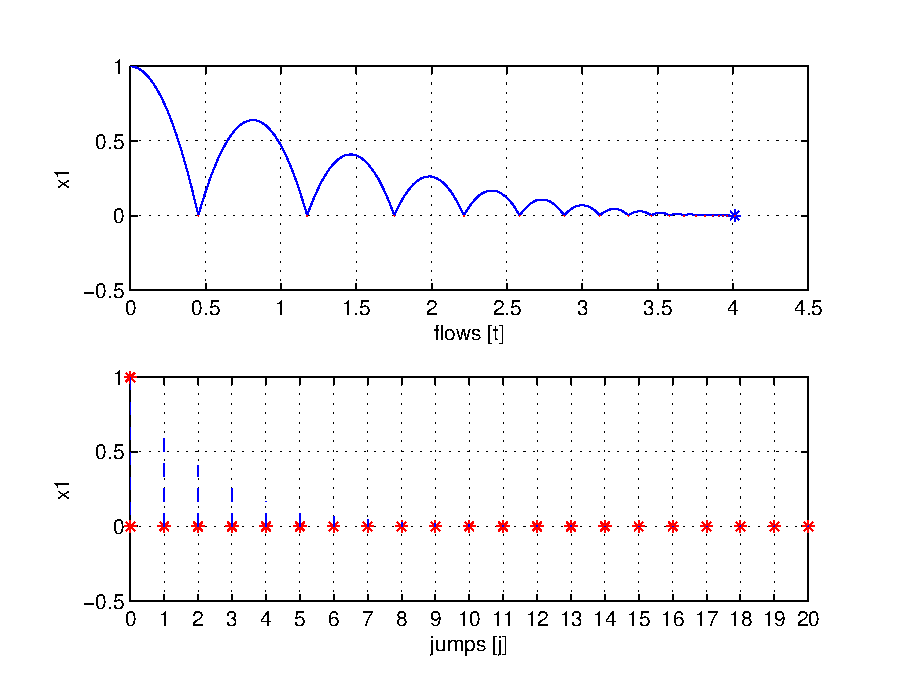
\includegraphics[width=.45\textwidth]{figures/Examples/FlowsAndJumps1lite.eps}
\label{fig:lite-1}}
\qquad
\subfigure[Velocity]{
    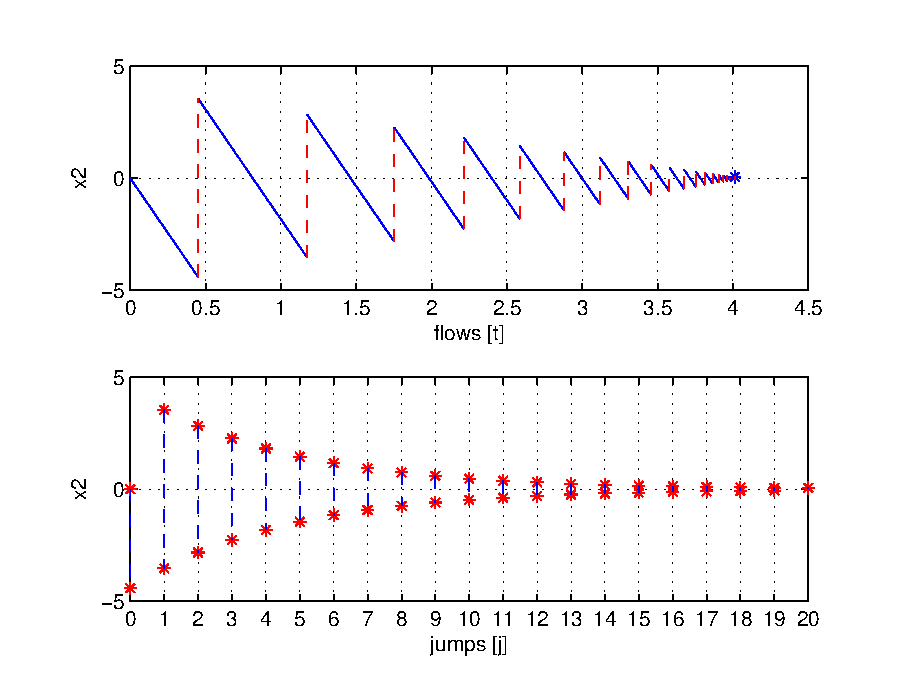
\includegraphics[width=.45\textwidth]{figures/Examples/FlowsAndJumps2lite.eps}
\label{fig:lite-2}}
\caption{Solution of Example \ref{ex:bblite}}
\end{figure}

\begin{figure}[ht]
  \begin{center}
  \psfrag{t}[c]{$t$}
  \psfrag{j}[c]{$j$}
  \psfrag{x1}[c]{$x_1$}
    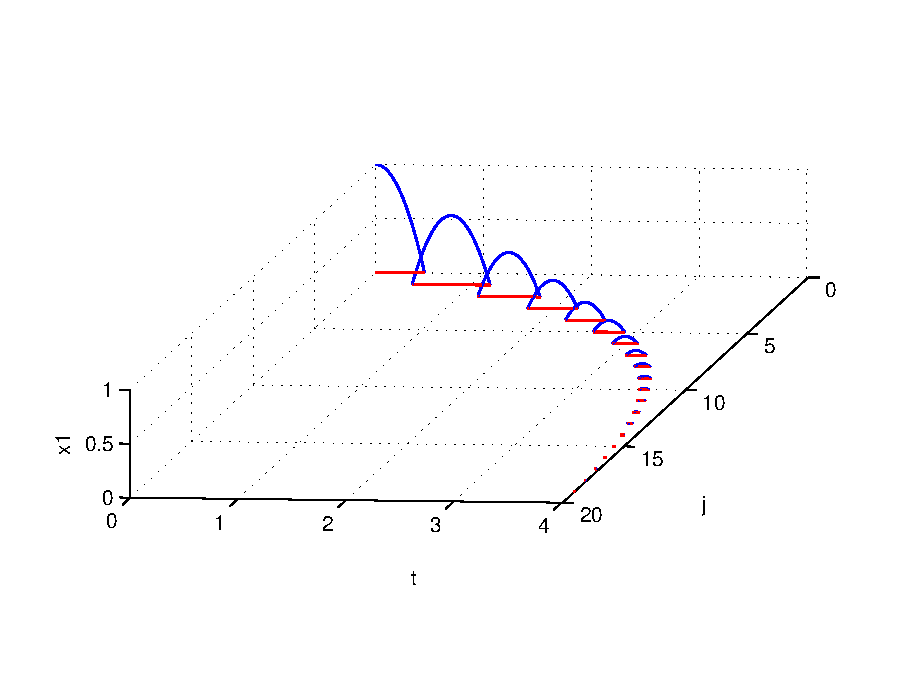
\includegraphics[width=.8\textwidth]{figures/Examples/HybridArclite.eps}
   \caption{Hybrid arc corresponding to a solution of Example~\ref{ex:bblite}: height}
\label{fig:lite-3}
  \end{center}
\end{figure}

A solution to the bouncing ball system from $x(0,0)=[1,0]^\top$ and with $TSPAN = [0 \hspace{2mm} 10], JSPAN = [0 \hspace{2mm} 20]$, $rule =1$, is depicted in Figure~\ref{fig:lite-1} (height) and Figure~\ref{fig:lite-2} (velocity).  Both the projection onto $t$ and $j$ are shown. Figure~\ref{fig:lite-3} depicts the corresponding hybrid arc for the position state.

For MATLAB files of this example, see Examples/Example\_\ref{ex:bblite}.

\end{example}


%% ADDED DETAILS OF \matlab{}-based CODE
\subsection{Solver Function}

%\ricardo{Perhaps add some text here to briefly describe what the functions implement?}

The solver function {\tt HyEQsolver} solves the hybrid system using 
three different functions as shown below. 
First, the flows are calculated using the built-in ODE solver function {\tt ODE45} in \matlab{}. 
If the solution leaves the flow set {\tt C}, the discrete event is detected using 
the function {\tt zeroevents} as shown in Section \ref{sec:eventsdetection}. When the state jumps, 
the next value of the state is calculated via the jump map {\tt g} using the function {\tt jump} 
as shown in Section \ref{sec:jumpmap}.\\

\codeLocation{Matlab2tex} 
% \code{HyEQsolver\_inst.m}
% % % This file was automatically created from the m-file 
% "m2tex.m" written by USL. 
% The fontencoding in this file is UTF-8. 
%  
% You will need to include the following two packages in 
% your LaTeX-Main-File. 
%  
% \usepackage{color} 
% \usepackage{fancyvrb} 
%  
% It is advised to use the following option for Inputenc 
% \usepackage[utf8]{inputenc} 
%  
  
% definition of matlab colors: 
\definecolor{mblue}{rgb}{0,0,1} 
\definecolor{mgreen}{rgb}{0.13333,0.5451,0.13333} 
\definecolor{mred}{rgb}{0.62745,0.12549,0.94118} 
\definecolor{mgrey}{rgb}{0.5,0.5,0.5} 
\definecolor{mdarkgrey}{rgb}{0.25,0.25,0.25} 
  
\DefineShortVerb[fontfamily=courier,fontseries=m]{\$} 
\DefineShortVerb[fontfamily=courier,fontseries=b]{\#} 
  
\begin{Verbatim}[commandchars=\$\{\},numbers=left,numbersep=2pt] 

    $textcolor{mblue}{function} [t j x] = HyEQsolver(f,g,C,D,x0,TSPAN,JSPAN,rule,options,solver,E) 
    $textcolor{mgreen}{%HYEQSOLVER solves hybrid equations.} 
    $textcolor{mgreen}{%   Syntax: [t j x] = HYEQSOLVER(f,g,C,D,x0,TSPAN,JSPAN,rule,options,solver,E)} 
    $textcolor{mgreen} 
    $textcolor{mgreen} 
    $textcolor{mgreen}{%   where x is the state, f is the flow map, g is the jump map, C is the} 
    $textcolor{mgreen}{%   flow set, and D is the jump set. It outputs the state trajectory (t,j)} 
    $textcolor{mgreen}{%   -> x(t,j), where t is the flow time parameter and j is the jump} 
    $textcolor{mgreen} 
    $textcolor{mgreen} 
    $textcolor{mgreen}{%   TSPAN = [TSTART TFINAL] is the time interval. JSPAN = [JSTART JSTOP] is} 
    $textcolor{mgreen}{%       the interval for discrete jumps. The algorithm stop when the first} 
    $textcolor{mgreen} 
    $textcolor{mgreen}{%   rule (optional parameter) - rule for jumps} 
    $textcolor{mgreen}{%       rule = 1 (default) -> priority for jumps rule = 2 -> priority for} 
    $textcolor{mgreen} 
    $textcolor{mgreen}{%   options (optional parameter) - options for the solver see odeset f.ex.} 
    $textcolor{mgreen}{%       options = odeset('RelTol',1e-6);} 
    $textcolor{mgreen} 
    $textcolor{mgreen}{%   solver (optional parameter. String) - selection of the desired ode} 
    $textcolor{mgreen}{%       solver. All ode solvers are suported, exept for ode15i.  See help} 
    $textcolor{mgreen} 
    $textcolor{mgreen}{%   E (optional parameter) - Mass matrix [constant matrix | function_handle]} 
    $textcolor{mgreen}{%       For problems: } 
    $textcolor{mgreen}{%       E*\dot{x} = f(x) x \in C } 
    $textcolor{mgreen}{%       x^+ = g(x)  x \in D} 
    $textcolor{mgreen}{%       set this property to the value of the constant mass matrix. For} 
    $textcolor{mgreen}{%       problems with time- or state-dependent mass matrices, set this} 
    $textcolor{mgreen}{%       property to a function that evaluates the mass matrix. See help} 
    $textcolor{mgreen} 
    $textcolor{mgreen} 
    $textcolor{mgreen}{%         % Consider the hybrid system model for the bouncing ball with data given in} 
    $textcolor{mgreen}{%         % Example 1.2. For this example, we consider the ball to be bouncing on a} 
    $textcolor{mgreen}{%         % floor at zero height. The constants for the bouncing ball system are} 
    $textcolor{mgreen}{%         % \gamma=9.81 and \lambda=0.8. The following procedure is used to} 
    $textcolor{mgreen}{%         % simulate this example in the Lite HyEQ Solver:} 
    $textcolor{mgreen}{%} 
    $textcolor{mgreen}{%         % * Inside the MATLAB script run_ex1_2.m, initial conditions, simulation} 
    $textcolor{mgreen}{%         % horizons, a rule for jumps, ode solver options, and a step size} 
    $textcolor{mgreen}{%         % coefficient are defined. The function HYEQSOLVER.m is called in order to} 
    $textcolor{mgreen}{%         % run the simulation, and a script for plotting solutions is included.} 
    $textcolor{mgreen}{%         % * Then the MATLAB functions f_ex1_2.m, C_ex1_2.m, g_ex1_2.m, D_ex1_2.m} 
    $textcolor{mgreen}{%         % are edited according to the data given below.} 
    $textcolor{mgreen}{%         % * Finally, the simulation is run by clicking the run button in} 
    $textcolor{mgreen}{%         % run_ex1_2.m or by calling run_ex1_2.m in the MATLAB command window.} 
    $textcolor{mgreen}{%} 
    $textcolor{mgreen}{%         % For further information, type in the command window:} 
    $textcolor{mgreen} 
    $textcolor{mgreen}{%         % Define initial conditions} 
    $textcolor{mgreen}{%         x1_0 = 1;} 
    $textcolor{mgreen}{%         x2_0 = 0;} 
    $textcolor{mgreen} 
    $textcolor{mgreen}{%         % Set simulation horizon} 
    $textcolor{mgreen}{%         TSPAN = [0 10];} 
    $textcolor{mgreen} 
    $textcolor{mgreen}{%         % Set rule for jumps and ODE solver options} 
    $textcolor{mgreen} 
    $textcolor{mgreen}{%         % rule = 1 -> priority for jumps} 
    $textcolor{mgreen} 
    $textcolor{mgreen}{%         % rule = 2 -> priority for flows} 
    $textcolor{mgreen} 
    $textcolor{mgreen}{%         % set the maximum step length. At each run of the} 
    $textcolor{mgreen}{%         % integrator the option 'MaxStep' is set to} 
    $textcolor{mgreen}{%         % (time length of last integration)*maxStepCoefficient.} 
    $textcolor{mgreen}{%         %  Default value = 0.1} 
    $textcolor{mgreen}{%} 
    $textcolor{mgreen} 
    $textcolor{mgreen} 
    $textcolor{mgreen}{%         % Simulate using the HYEQSOLVER script} 
    $textcolor{mgreen}{%         % Given the matlab functions that models the flow map, jump map,} 
    $textcolor{mgreen}{%         % flow set and jump set (f_ex1_2, g_ex1_2, C_ex1_2, and D_ex1_2} 
    $textcolor{mgreen}{%         % respectively)} 
    $textcolor{mgreen}{%} 
    $textcolor{mgreen}{%         [t j x] = HYEQSOLVER( @f_ex1_2,@g_ex1_2,@C_ex1_2,@D_ex1_2,...} 
    $textcolor{mgreen} 
    $textcolor{mgreen}{%         % plot solution} 
    $textcolor{mgreen}{%} 
    $textcolor{mgreen}{%         figure(1) % position} 
    $textcolor{mgreen}{%         clf} 
    $textcolor{mgreen}{%         subplot(2,1,1),plotflows(t,j,x(:,1))} 
    $textcolor{mgreen}{%         grid on} 
    $textcolor{mgreen} 
    $textcolor{mgreen}{%         subplot(2,1,2),plotjumps(t,j,x(:,1))} 
    $textcolor{mgreen}{%         grid on} 
    $textcolor{mgreen} 
    $textcolor{mgreen}{%         figure(2) % velocity} 
    $textcolor{mgreen}{%         clf} 
    $textcolor{mgreen}{%         subplot(2,1,1),plotflows(t,j,x(:,2))} 
    $textcolor{mgreen}{%         grid on} 
    $textcolor{mgreen} 
    $textcolor{mgreen}{%         subplot(2,1,2),plotjumps(t,j,x(:,2))} 
    $textcolor{mgreen}{%         grid on} 
    $textcolor{mgreen} 
    $textcolor{mgreen}{%         % plot hybrid arc} 
    $textcolor{mgreen}{%         } 
    $textcolor{mgreen}{%         figure(3)} 
    $textcolor{mgreen}{%         plotHybridArc(t,j,x)} 
    $textcolor{mgreen}{%         xlabel('j')} 
    $textcolor{mgreen}{%         ylabel('t')} 
    $textcolor{mgreen} 
    $textcolor{mgreen}{%         % plot solution using plotHarc and plotHarcColor} 
    $textcolor{mgreen}{%} 
    $textcolor{mgreen}{%         figure(4) % position} 
    $textcolor{mgreen}{%         clf} 
    $textcolor{mgreen}{%         subplot(2,1,1), plotHarc(t,j,x(:,1));} 
    $textcolor{mgreen}{%         grid on} 
    $textcolor{mgreen}{%         ylabel('x_1 position')} 
    $textcolor{mgreen}{%         subplot(2,1,2), plotHarc(t,j,x(:,2));} 
    $textcolor{mgreen}{%         grid on} 
    $textcolor{mgreen} 
    $textcolor{mgreen}{%} 
    $textcolor{mgreen}{%         % plot a phase plane} 
    $textcolor{mgreen}{%         figure(5) % position} 
    $textcolor{mgreen}{%         clf} 
    $textcolor{mgreen}{%         plotHarcColor(x(:,1),j,x(:,2),t);} 
    $textcolor{mgreen}{%         xlabel('x_1')} 
    $textcolor{mgreen}{%         ylabel('x_2')} 
    $textcolor{mgreen} 
    $textcolor{mgreen}{%--------------------------------------------------------------------------} 
    $textcolor{mgreen}{% Matlab M-file Project: HyEQ Toolbox @  Hybrid Systems Laboratory (HSL),} 
    $textcolor{mgreen}{% https://hybrid.soe.ucsc.edu/software} 
    $textcolor{mgreen}{% http://hybridsimulator.wordpress.com/} 
    $textcolor{mgreen}{% Filename: HYEQSOLVER.m} 
    $textcolor{mgreen}{%--------------------------------------------------------------------------} 
    $textcolor{mgreen}{%   See also HYEQSOLVER, PLOTARC, PLOTARC3, PLOTFLOWS, PLOTHARC,} 
    $textcolor{mgreen}{%   PLOTHARCCOLOR, PLOTHARCCOLOR3D, PLOTHYBRIDARC, PLOTJUMPS.} 
    $textcolor{mgreen}{%   Copyright @ Hybrid Systems Laboratory (HSL),} 
    $textcolor{mgreen}{%   Revision: 0.0.0.4 Date: 04/6/2017 16:26:00} 
     
     
    $textcolor{mblue}{if} ~exist($textcolor{mred}{'rule'},$textcolor{mred}{'var'}) 
        rule = 1; 
    $textcolor{mblue}{end} 
     
    $textcolor{mblue}{if} ~exist($textcolor{mred}{'options'},$textcolor{mred}{'var'}) 
        options = odeset(); 
    $textcolor{mblue}{end} 
    $textcolor{mblue}{if} exist($textcolor{mred}{'E'},$textcolor{mred}{$textcolor{mred}{'var'}}) && ~exist($textcolor{mred}{'solver'},$textcolor{mred}{$textcolor{mred}{'var'}}) 
        solver = $textcolor{mred}{'ode15s'}; 
    $textcolor{mblue}{end} 
    $textcolor{mblue}{if} ~exist($textcolor{mred}{'solver'},$textcolor{mred}{'var'}) 
        solver = $textcolor{mred}{'ode45'}; 
    $textcolor{mblue}{end} 
    $textcolor{mblue}{if} ~exist($textcolor{mred}{'E'},$textcolor{mred}{'var'}) 
        E = []; 
    $textcolor{mblue}{end} 
    $textcolor{mgreen}{% mass matrix (if existent)} 
    isDAE = false; 
    $textcolor{mblue}{if} ~isempty(E) 
        isDAE = true; 
        $textcolor{mblue}{switch} isa(E,$textcolor{mred}{'function_handle'}) 
            $textcolor{mblue}{case} true $textcolor{mgreen}{% Function E(x)} 
                M = E; 
                options = odeset(options,$textcolor{mred}{'Mass'},M,$textcolor{mred}{'Stats'},$textcolor{mred}{'off'},... 
                    $textcolor{mred}{'MassSingular'},$textcolor{mred}{'maybe'},$textcolor{mred}{'MStateDependence'},$textcolor{mred}{'strong'},... 
                    $textcolor{mred}{'InitialSlope'},f_hdae(x0,TSPAN(1)));  
            $textcolor{mblue}{case} false $textcolor{mgreen}{% Constant double matrix} 
                M = double(E); 
                options = odeset(options,$textcolor{mred}{'Mass'},M,$textcolor{mred}{'Stats'},$textcolor{mred}{'off'},... 
                    $textcolor{mred}{'MassSingular'},$textcolor{mred}{'maybe'},$textcolor{mred}{'MStateDependence'},$textcolor{mred}{'none'}); 
        $textcolor{mblue}{end} 
    $textcolor{mblue}{end} 
     
    odeX = str2func(solver); 
    nargf = nargin(f); 
    nargg = nargin(g); 
    nargC = nargin(C); 
    nargD = nargin(D); 
     
     
     
    $textcolor{mgreen}{% simulation horizon} 
    tstart = TSPAN(1); 
    tfinal = TSPAN(end); 
    jout = JSPAN(1); 
    j = jout(end); 
     
    $textcolor{mgreen}{% simulate} 
    tout = tstart; 
    [rx,cx] = size(x0); 
    $textcolor{mblue}{if} rx == 1 
        xout = x0; 
    $textcolor{mblue}{elseif} cx == 1 
        xout = x0.'; 
    $textcolor{mblue}{else} 
        error($textcolor{mred}{'Error, x0 does not have the proper size'}) 
    $textcolor{mblue}{end} 
     
    $textcolor{mgreen}{% Jump if jump is prioritized:} 
    $textcolor{mblue}{if} rule == 1 
        $textcolor{mblue}{while} (j<JSPAN(end)) 
            $textcolor{mgreen}{% Check if value it is possible to jump current position} 
            insideD = fun_wrap(xout(end,:).',tout(end),j,D,nargD); 
            $textcolor{mblue}{if} insideD == 1 
                [j $textcolor{mred}{tout jout xout] = jump(g,j,tout,jout,xout,nargg);} 
            $textcolor{mblue}{else} 
                break; 
            $textcolor{mblue}{end} 
        $textcolor{mblue}{end} 
    $textcolor{mblue}{end} 
    fprintf($textcolor{mred}{'Completed: %3.0f%%'},0); 
    $textcolor{mblue}{while} (j < JSPAN(end) && tout(end) < TSPAN(end)) 
        options = odeset(options,$textcolor{mred}{'Events'},@(t,x) zeroevents(x,t,j,C,D,... 
            rule,nargC,nargD)); 
        $textcolor{mgreen}{% Check if it is possible to flow from current position} 
        insideC = fun_wrap(xout(end,:).',tout(end),j,C,nargC); 
        $textcolor{mblue}{if} insideC == 1 
            $textcolor{mblue}{if} isDAE 
                options = odeset(options,$textcolor{mred}{'InitialSlope'},f(xout(end,:).',tout(end))); 
            $textcolor{mblue}{end} 
            [t,x] = odeX(@(t,x) fun_wrap(x,t,j,f,nargf),[tout(end) tfinal],... 
                xout(end,:).', $textcolor{mred}{options);} 
            nt = length(t); 
            tout = [tout; t]; 
            xout = [xout; x]; 
            jout = [jout; j*ones(1,nt)']; 
        $textcolor{mblue}{end} 
         
        $textcolor{mgreen}{%Check if it is possible to jump} 
        insideD = fun_wrap(xout(end,:).',tout(end),j,D,nargD); 
        $textcolor{mblue}{if} insideD == 0 
            break; 
        $textcolor{mblue}{else} 
            $textcolor{mblue}{if} rule == 1 
                $textcolor{mblue}{while} (j<JSPAN(end)) 
                    $textcolor{mgreen}{% Check if it is possible to jump from current position} 
                    insideD = fun_wrap(xout(end,:).',tout(end),j,D,nargD); 
                    $textcolor{mblue}{if} insideD == 1 
                        [j $textcolor{mred}{tout jout xout] = jump(g,j,tout,jout,xout,nargg);} 
                    $textcolor{mblue}{else} 
                        break; 
                    $textcolor{mblue}{end} 
                $textcolor{mblue}{end} 
            $textcolor{mblue}{else} 
                [j $textcolor{mred}{tout jout xout] = jump(g,j,tout,jout,xout,nargg);} 
            $textcolor{mblue}{end} 
        $textcolor{mblue}{end} 
        fprintf($textcolor{mred}{'\b\b\b\b%3.0f%%'},max(100*j/JSPAN(end),100*tout(end)/TSPAN(end))); 
    $textcolor{mblue}{end} 
    t = tout; 
    x = xout; 
    j = jout; 
    fprintf($textcolor{mred}{'\nDone\n'}); 
    $textcolor{mblue}{end} 
      
\end{Verbatim}  
  
\UndefineShortVerb{\$} 
\UndefineShortVerb{\#} 
 
% \label{scr:HyEQsolver}

% \subsubsection{Events Detection}
% \label{sec:eventsdetection}

% \code{zeroevents\_inst.m}
% % % This file was automatically created from the m-file 
% "m2tex.m" written by USL. 
% The fontencoding in this file is UTF-8. 
%  
% You will need to include the following two packages in 
% your LaTeX-Main-File. 
%  
% \usepackage{color} 
% \usepackage{fancyvrb} 
%  
% It is advised to use the following option for Inputenc 
% \usepackage[utf8]{inputenc} 
%  
  
% definition of matlab colors: 
\definecolor{mblue}{rgb}{0,0,1} 
\definecolor{mgreen}{rgb}{0.13333,0.5451,0.13333} 
\definecolor{mred}{rgb}{0.62745,0.12549,0.94118} 
\definecolor{mgrey}{rgb}{0.5,0.5,0.5} 
\definecolor{mdarkgrey}{rgb}{0.25,0.25,0.25} 
  
\DefineShortVerb[fontfamily=courier,fontseries=m]{\$} 
\DefineShortVerb[fontfamily=courier,fontseries=b]{\#} 
  
\begin{Verbatim}[commandchars=\$\{\},numbers=left,numbersep=2pt] 

    $textcolor{mblue}{function} [value,isterminal,direction] = zeroevents(x,t,j,C,D,rule,nargC,nargD) 
    $textcolor{mblue}{switch} rule 
        $textcolor{mblue}{case} 1 $textcolor{mgreen}{% -> priority for jumps} 
            isterminal(1) = 1; $textcolor{mgreen}{% InsideC} 
            isterminal(2) = 1; $textcolor{mgreen}{% Inside(C \cap D)} 
            isterminal(3) = 1; $textcolor{mgreen}{% OutsideC} 
            direction(1) = -1; $textcolor{mgreen}{% InsideC} 
            direction(2) = -1; $textcolor{mgreen}{% Inside(C \cap D)} 
            direction(3) =  1; $textcolor{mgreen}{% OutsideC} 
        $textcolor{mblue}{case} 2 $textcolor{mgreen}{%(default) -> priority for flows} 
            isterminal(1) = 1; $textcolor{mgreen}{% InsideC} 
            isterminal(2) = 0; $textcolor{mgreen}{% Inside(C \cap D)} 
            isterminal(3) = 1; $textcolor{mgreen}{% OutsideC} 
            direction(1) = -1; $textcolor{mgreen}{% InsideC} 
            direction(2) = -1; $textcolor{mgreen}{% Inside(C \cap D)} 
            direction(3) =  1; $textcolor{mgreen}{% OutsideC} 
    $textcolor{mblue}{end} 
     
    insideC = fun_wrap(x,t,j,C,nargC); 
    insideD = fun_wrap(x,t,j,D,nargD); 
    outsideC = -fun_wrap(x,t,j,C,nargC); 
     
     
    value(1) = 2*insideC; 
    value(2) = 2-insideC - insideD; 
    value(3) = 2*outsideC; 
     
    $textcolor{mblue}{end} 
      
\end{Verbatim}  
  
\UndefineShortVerb{\$} 
\UndefineShortVerb{\#} 
 
% \label{scr:zeroevents}

% \subsubsection{Jump Map}
% \label{sec:jumpmap}

% \code{jump\_inst.m}
% % % This file was automatically created from the m-file 
% "m2tex.m" written by USL. 
% The fontencoding in this file is UTF-8. 
%  
% You will need to include the following two packages in 
% your LaTeX-Main-File. 
%  
% \usepackage{color} 
% \usepackage{fancyvrb} 
%  
% It is advised to use the following option for Inputenc 
% \usepackage[utf8]{inputenc} 
%  
  
% definition of matlab colors: 
\definecolor{mblue}{rgb}{0,0,1} 
\definecolor{mgreen}{rgb}{0.13333,0.5451,0.13333} 
\definecolor{mred}{rgb}{0.62745,0.12549,0.94118} 
\definecolor{mgrey}{rgb}{0.5,0.5,0.5} 
\definecolor{mdarkgrey}{rgb}{0.25,0.25,0.25} 
  
\DefineShortVerb[fontfamily=courier,fontseries=m]{\$} 
\DefineShortVerb[fontfamily=courier,fontseries=b]{\#} 
  
\noindent          
 \hspace*{-1.6em}{\scriptsize 1}$  $\color{mblue}$function$\color{black}$ [j tout jout xout] = jump(g,j,tout,jout,xout,nargfun)$\\
 \hspace*{-1.6em}{\scriptsize 2}$  $\color{mgreen}$% Jump$\color{black}$$\\
 \hspace*{-1.6em}{\scriptsize 3}$  j = j+1;$\\
 \hspace*{-1.6em}{\scriptsize 4}$  y = fun_wrap(xout(end,:).',tout(end),jout(end),g,nargfun); $\\
 \hspace*{-1.6em}{\scriptsize 5}$  $\color{mgreen}$% Save results$\color{black}$$\\
 \hspace*{-1.6em}{\scriptsize 6}$  tout = [tout; tout(end)];$\\
 \hspace*{-1.6em}{\scriptsize 7}$  xout = [xout; y.'];$\\
 \hspace*{-1.6em}{\scriptsize 8}$  jout = [jout; j];$\\
 \hspace*{-1.6em}{\scriptsize 9}$  $\color{mblue}$end$\color{black}$$\\
 \hspace*{-2em}{\scriptsize 10}$  $\\ 
  
\UndefineShortVerb{\$} 
\UndefineShortVerb{\#}
% \label{scr:jump}

% \subsubsection{Function Wrapper}
% \label{sec:funwrapp}

% \code{fun\_wrap\_inst.m}
% % % This file was automatically created from the m-file 
% "m2tex.m" written by USL. 
% The fontencoding in this file is UTF-8. 
%  
% You will need to include the following two packages in 
% your LaTeX-Main-File. 
%  
% \usepackage{color} 
% \usepackage{fancyvrb} 
%  
% It is advised to use the following option for Inputenc 
% \usepackage[utf8]{inputenc} 
%  
  
% definition of matlab colors: 
\definecolor{mblue}{rgb}{0,0,1} 
\definecolor{mgreen}{rgb}{0.13333,0.5451,0.13333} 
\definecolor{mred}{rgb}{0.62745,0.12549,0.94118} 
\definecolor{mgrey}{rgb}{0.5,0.5,0.5} 
\definecolor{mdarkgrey}{rgb}{0.25,0.25,0.25} 
  
\DefineShortVerb[fontfamily=courier,fontseries=m]{\$} 
\DefineShortVerb[fontfamily=courier,fontseries=b]{\#} 
  
\begin{Verbatim}[commandchars=\$\{\},numbers=left,numbersep=2pt] 

    $textcolor{mblue}{function} xdelta = fun_wrap(x,t,j,h,nargfun) 
    $textcolor{mgreen}{%fun_wrap   Variable input arguments function (easy use for users).} 
    $textcolor{mgreen}{%   fun_wrap(x,t,j,h,nargfun) depending on the function h written by the} 
    $textcolor{mgreen}{%   user, this script selects how the HyEQ solver should call that} 
    $textcolor{mgreen}{%   function.} 
    $textcolor{mgreen}{%    x: state} 
    $textcolor{mgreen}{%    t: time} 
    $textcolor{mgreen}{%    j: discrete time} 
    $textcolor{mgreen}{%    h: function handle} 
    $textcolor{mgreen}{%    nargfun: number of input arguments of function h    } 
    $textcolor{mgreen}{%--------------------------------------------------------------------------} 
    $textcolor{mgreen}{% Matlab M-file Project: HyEQ Toolbox @  Hybrid Systems Laboratory (HSL), } 
    $textcolor{mgreen}{% https://hybrid.soe.ucsc.edu/software} 
    $textcolor{mgreen}{% http://hybridsimulator.wordpress.com/} 
    $textcolor{mgreen}{% Filename: fun_wrap.m} 
    $textcolor{mgreen}{%--------------------------------------------------------------------------} 
    $textcolor{mgreen}{%   See also HYEQSOLVER, PLOTARC, PLOTARC3, PLOTFLOWS, PLOTHARC,} 
    $textcolor{mgreen}{%   PLOTHARCCOLOR, PLOTHARCCOLOR3D, PLOTHYBRIDARC, PLOTJUMPS.} 
    $textcolor{mgreen}{%   Copyright @ Hybrid Systems Laboratory (HSL),} 
    $textcolor{mgreen}{%   Revision: 0.0.0.3 Date: 01/28/2016 5:12:00} 
     
     
    $textcolor{mblue}{switch} nargfun 
        $textcolor{mblue}{case} 1 
            xdelta = h(x); 
        $textcolor{mblue}{case} 2 
            xdelta = h(x,t); 
        $textcolor{mblue}{case} 3 
            xdelta = h(x,t,j);         
    $textcolor{mblue}{end} 
    $textcolor{mblue}{end}  
\end{Verbatim}  
  
\UndefineShortVerb{\$} 
\UndefineShortVerb{\#} 
 
% \label{scr:funwrapp}

\subsection{Software Requirements}

In order to run simulations using the \matlab{}-based HyEQ Simulator, 
\matlab{}~R2014b or newer is required.

\subsection{Configuration of Solver}

Before a simulation is started, it is important to determine the needed integrator scheme, 
zero-cross detection settings, precision, and other tolerances. 
Using the default settings does not always give the most efficient or most accurate simulations.
In the \matlab{}-based HyEQ Simulator, these parameters are edited in the {\tt run.m} file using

\begin{verbatim} options = odeset('RelTol',1e-6,'MaxStep',0.1);. \end{verbatim}

\subsection{Initialization}

%\ricardo{Perhaps expand this as the HyEQ Simulator?}

The \matlab{}-based HyEQ Simulator is initialized and run by calling the function {\tt run.m}. 
Inside {\tt run.m}, the initial conditions, simulation horizons {\tt TSPAN} 
and {\tt JSPAN}, a rule for jumps, and simulation tolerances are defined. 
After all of the parameters are defined, the function {\tt HyEQsolver} is called, 
and the simulation runs. See below for sample code to initialize and run the bouncing ball example, 
Example ~\ref{ex:bblite}.\\

\codeLocation{Matlab2tex} 
\code{initialization\_inst.m}
% % This file was automatically created from the m-file 
% "m2tex.m" written by USL. 
% The fontencoding in this file is UTF-8. 
%  
% You will need to include the following two packages in 
% your LaTeX-Main-File. 
%  
% \usepackage{color} 
% \usepackage{fancyvrb} 
%  
% It is advised to use the following option for Inputenc 
% \usepackage[utf8]{inputenc} 
%  
  
% definition of matlab colors: 
\definecolor{mblue}{rgb}{0,0,1} 
\definecolor{mgreen}{rgb}{0.13333,0.5451,0.13333} 
\definecolor{mred}{rgb}{0.62745,0.12549,0.94118} 
\definecolor{mgrey}{rgb}{0.5,0.5,0.5} 
\definecolor{mdarkgrey}{rgb}{0.25,0.25,0.25} 
  
\DefineShortVerb[fontfamily=courier,fontseries=m]{\$} 
\DefineShortVerb[fontfamily=courier,fontseries=b]{\#} 
  
\noindent              
 \hspace*{-1.6em}{\scriptsize 1}$  $\color{mgreen}$% initial conditions$\color{black}$$\\
 \hspace*{-1.6em}{\scriptsize 2}$  x1_0 = 1;$\\
 \hspace*{-1.6em}{\scriptsize 3}$  x2_0 = 0;$\\
 \hspace*{-1.6em}{\scriptsize 4}$  x0 = [x1_0;x2_0];$\\
 \hspace*{-1.6em}{\scriptsize 5}$  $\color{mgreen}$% simulation horizon$\color{black}$$\\
 \hspace*{-1.6em}{\scriptsize 6}$  TSPAN=[0,10];$\\
 \hspace*{-1.6em}{\scriptsize 7}$  JSPAN = [0,20];$\\
 \hspace*{-1.6em}{\scriptsize 8}$  $\color{mgreen}$% rule for jumps$\color{black}$$\\
 \hspace*{-1.6em}{\scriptsize 9}$  $\color{mgreen}$% rule = 1 -> priority for jumps$\color{black}$$\\
 \hspace*{-2em}{\scriptsize 10}$  $\color{mgreen}$% rule = 2 -> priority for flows$\color{black}$$\\
 \hspace*{-2em}{\scriptsize 11}$  rule = 1;$\\
 \hspace*{-2em}{\scriptsize 12}$  options = odeset($\color{mred}$'RelTol'$\color{black}$,1e-6,$\color{mred}$'MaxStep'$\color{black}$,.1);$\\
 \hspace*{-2em}{\scriptsize 13}$  $\color{mgreen}$% simulate$\color{black}$$\\
 \hspace*{-2em}{\scriptsize 14}$  [t,j,x] = HyEQsolver(@f,@g,@C,@D,x0,TSPAN,JSPAN,rule,options);$\\ 
  
\UndefineShortVerb{\$} 
\UndefineShortVerb{\#}
\label{scr:initialization}


\subsection{Postprocessing and Plotting solutions}\label{sec:plotfcn}

The function {\tt run.m} is also used to plot solutions after the simulations is complete. 
See below for sample code to plot solutions to the bouncing ball example, Example~\ref{ex:bblite}.

\code{postprocesing\_inst.m}
% % This file was automatically created from the m-file 
% "m2tex.m" written by USL. 
% The fontencoding in this file is UTF-8. 
%  
% You will need to include the following two packages in 
% your LaTeX-Main-File. 
%  
% \usepackage{color} 
% \usepackage{fancyvrb} 
%  
% It is advised to use the following option for Inputenc 
% \usepackage[utf8]{inputenc} 
%  
  
% definition of matlab colors: 
\definecolor{mblue}{rgb}{0,0,1} 
\definecolor{mgreen}{rgb}{0.13333,0.5451,0.13333} 
\definecolor{mred}{rgb}{0.62745,0.12549,0.94118} 
\definecolor{mgrey}{rgb}{0.5,0.5,0.5} 
\definecolor{mdarkgrey}{rgb}{0.25,0.25,0.25} 
  
\DefineShortVerb[fontfamily=courier,fontseries=m]{\$} 
\DefineShortVerb[fontfamily=courier,fontseries=b]{\#} 
  
\begin{Verbatim}[commandchars=\$\{\},numbers=left,numbersep=2pt] 

    $textcolor{mgreen}{% plot solution} 
    figure(1) $textcolor{mgreen}{% position} 
    clf 
    subplot(2,1,1),plotflows(t,j,x(:,1)) 
    grid $textcolor{mred}{on} 
    ylabel($textcolor{mred}{'x1'}) 
    subplot(2,1,2),plotjumps(t,j,x(:,1)) 
    grid $textcolor{mred}{on} 
    ylabel($textcolor{mred}{'x1'}) 
    figure(2) $textcolor{mgreen}{% velocity} 
    clf 
    subplot(2,1,1),plotflows(t,j,x(:,2)) 
    grid $textcolor{mred}{on} 
    ylabel($textcolor{mred}{'x2'}) 
    subplot(2,1,2),plotjumps(t,j,x(:,2)) 
    grid $textcolor{mred}{on} 
    ylabel($textcolor{mred}{'x2'}) 
    $textcolor{mgreen}{% plot hybrid arc} 
    figure(2) 
    plotHybridArc(t,j,x) 
    xlabel($textcolor{mred}{'j'}) 
    ylabel($textcolor{mred}{'t'}) 
    zlabel($textcolor{mred}{'x1'}) 
    grid $textcolor{mred}{on} 
    view(37.5,30)  
\end{Verbatim}  
  
\UndefineShortVerb{\$} 
\UndefineShortVerb{\#} 
 
\label{scr:postprocesing}

\noindent The following functions are used to generate the plots:
{\color{red} TODO: Add info about plotting.}
% \begin{itemize}
% \item plotarc(t,j,x,L,jstar,modificatorF,modificatorJ,resolution,DDD,true3D): 
% plots the hybrid time domain (matrix) $(t,j)$ versus the sate $x$ 
% (matrix) taking into account jumps $j$. If $x$ is a matrix ($n$ states), 
% then the hybrid time is plotted versus the rows or columns of the matrix, 
% whichever line up. If $t$ and $j$ are a matrices, then each column of $x$ 
% will be plotted according to the hybrid time domain composed for each column of $t$ and $j$. 
% Depending on the input data, this function is capable of plotting several types of figures, 
% e.g., 2D, 3D, hybrid arcs with color, etc. 
% Next, we list several functions that specialize different types of plotting styles from plotarc. 
% For more information, please type $>>$ help plotarc or $>>$ helpwin plotarc in the command window.
% \item plotarc3(t,j,x,L,jstar,modificatorF,modificatorJ,resolution,true3D) 
% is a version of plotarc that specializes in figures in 3D. 
% For more information, please type $>>$ help plotarc3 or $>>$ helpwin plotarc3 in the command window.
% \item plotflows(t,j,x,$jstar$,resolution): plots (in blue) the projection of the
%   trajectory $x$ onto the flow time axis $t$.  The value of the
%   trajectory for intervals $[t_j,t_{j+1}]$ with empty interior is
%   marked with $*$ (in blue).  Dashed lines (in red) connect the value of the
%   trajectory before and after the jump. 
%   Figure~\ref{fig:input-1} shows a plot created with this function.
%  \begin{itemize}
%  	\item plotflows(t,j,x,$jstar$): The plot is cut regarding the $jstar$ interval ($jstar = [j-initial j-final]$).
% 	\item plotflows(t,j,x,$jstar$,resolution): Also, a maximum resolution in between jumps 
%   is given by the input variable resolution
%  \end{itemize}
% \item plotjumps(t,j,x,$jstar$,resolution): plots (in red) the projection of the
%   trajectory $x$ onto the jump time $j$. The initial and final value
%   of the trajectory on each interval $[t_j,t_{j+1}]$ is denoted by
%   $*$ (in red) and the continuous evolution of the trajectory on
%   each interval is depicted with a dashed line (in blue). 
%   Figure~\ref{fig:input-1} shows a plot created with this function.
%  \begin{itemize}
%  	\item plotjumps(t,j,x,$jstar$): The plot is cut regarding the $jstar$ interval ($jstar = [j-initial j-final]$).
% 	\item plotjumps(t,j,x,$jstar$,resolution): 
%         Also, a maximum resolution in between jumps is given by the input variable resolution.
%  \end{itemize}

% \item plotHybridArc(t,j,x,$jstar$,resolution): plots (in blue and red) the trajectory $x$ on hybrid
%       time domains. The intervals $[t_j,t_{j+1}]$ indexed by the
%       corresponding $j$ are depicted in the $t-j$ plane (in red). 
% Figure~\ref{fig:input-3} shows a plot created with this function.
%  \begin{itemize}
%  	\item plotHybridArc(t,j,x,$jstar$): 
%         The plot is cut regarding the $jstar$ interval ($jstar = [j-initial j-final]$).
% 	\item plotHybridArc(t,j,x,$jstar$,resolution): 
%         Also, a maximum resolution in between jumps is given by the input variable resolution.
%  \end{itemize}

% \item plotHarc(t,j,x,$jstar$,modificatorF, modificatorJ, resolution) is a function for plotting hybrid arcs (n states).
% \begin{itemize}
% \item plotHarc(t,j,x): plots the trajectory $x$ versus the hybrid time domain $(t,j)$.
%  If $x$ is a matrix, then the time vector is plotted versus the rows or columns of the matrix, 
% whichever line up.
% \item plotHarc(t,j,x,$jstar$): plots the trajectory $x$ versus the hybrid time domain $(t,j)$, 
% and the plot is cut regarding the $jstar$ interval $(jstar = [j_{initial},j_{final}])$.
% \item plotHarc(t,j,x,$jstar$, modificatorF,modificatorJ): 
% ModificatorF and ModificatorJ are cell arrays that contains the standard matlab 
% ploting modificators (type $>>$ help plotHarc or $>>$ 
% helpwin plotHarc in the command window for more information).
% \end{itemize}

% \item plotHarcColor(t,j,x,L,$jstar$,resolution) plots the trajectory 
% $x$ on hybrid time domain with color.
% \begin{itemize}
% \item plotHarcColor(t,j,x,L): plots the trajectory $x$ (vector) 
% versus the hybrid time domain $(t,j)$. The hybrid arc is plotted with $L$ data as color. The input vectors $t,\ j,\ x,\ L$ must have the same length. 
% \item      plotHarcColor(t,j,x,L,$jstar$): If a specific interval in $j$ is required, $jstar = [j_{initial},
%  j_{final}]$ must be provided. (type $>>$ help plotHarcColor or $>>$ helpwin plotHarcColor in the command window for more information)
% \end{itemize}

% \item plotHarcColor3D(t,j,x,L,$jstar$,modificator,resolution) plots an $3D$ hybrid arc with color.
% \begin{itemize}
% \item plotHarcColor3D(t,j,x,L) plots the trajectory $x$ (3 states) taking into account the hybrid time domain $(t,j)$. 
% The hybrid arc is plotted with $L$ data as color. 
% The input vectors $t,\ j,\ x,\ L$ must have the same length and $x$ must have three columns.
% \item plotHarcColor3D(t,j,x,L,$jstar$) If a specific interval in $j$ is required, $jstar = [j_{initial},
%  j_{final}]$ must be provided.
%  \item plotHarcColor3D(t,j,x,L,$jstar$,modificator) Modificator is a cell array that contains 
% the standard matlab ploting modificators (type $>>$ help plotHarcColor3D or
% $>>$ helpwin plotHarcColor3D in the command window for more information).
% \end{itemize}
% \end{itemize}

\section{Simulink-based Hybrid Equation Simulator}
\label{sec:HyEQsimulator}

The HyEQ Toolbox includes three main Simulink library blocks that allow for simulation of 
a hybrid system $\HS =(C,f,D,g)$ using either externally defined functions or embedded 
\matlab{} functions, and a single hybrid system or interconnected hybrid systems with 
inputs using embedded \matlab{} functions. Figure~\ref{fig:Simulinklibblocks} 
shows these blocks in the Simulink Library Browser.

\begin{figure}[ht]
  \begin{center}
    {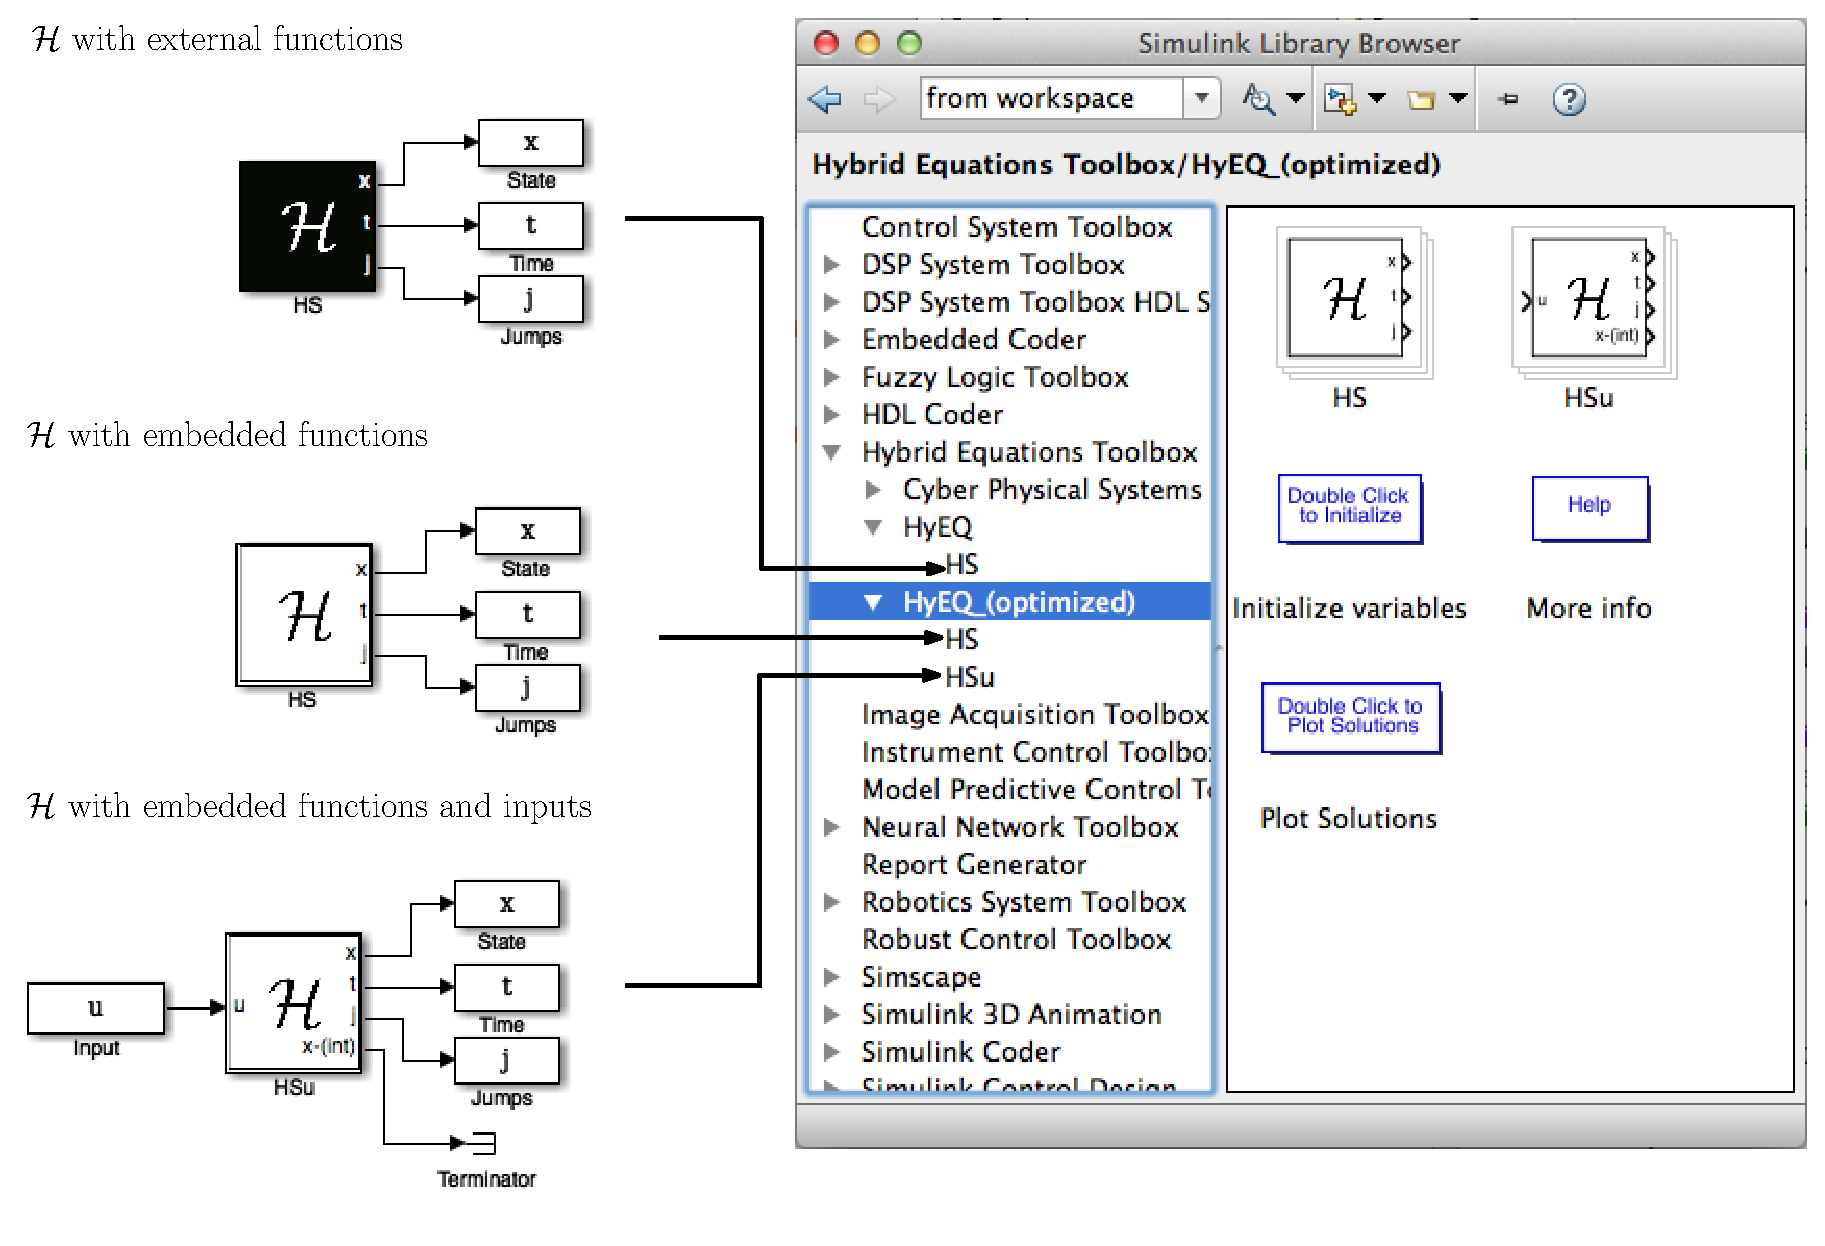
\includegraphics[width=1\textwidth]{figures/Simulink/SimulinkimplementationMac.eps}}
\caption{\matlab{}/Simulink library blocks for Simulink implementation.}
\label{fig:Simulinklibblocks}
  \end{center}
\end{figure}

\begin{figure}[ht]
  \begin{center}
    {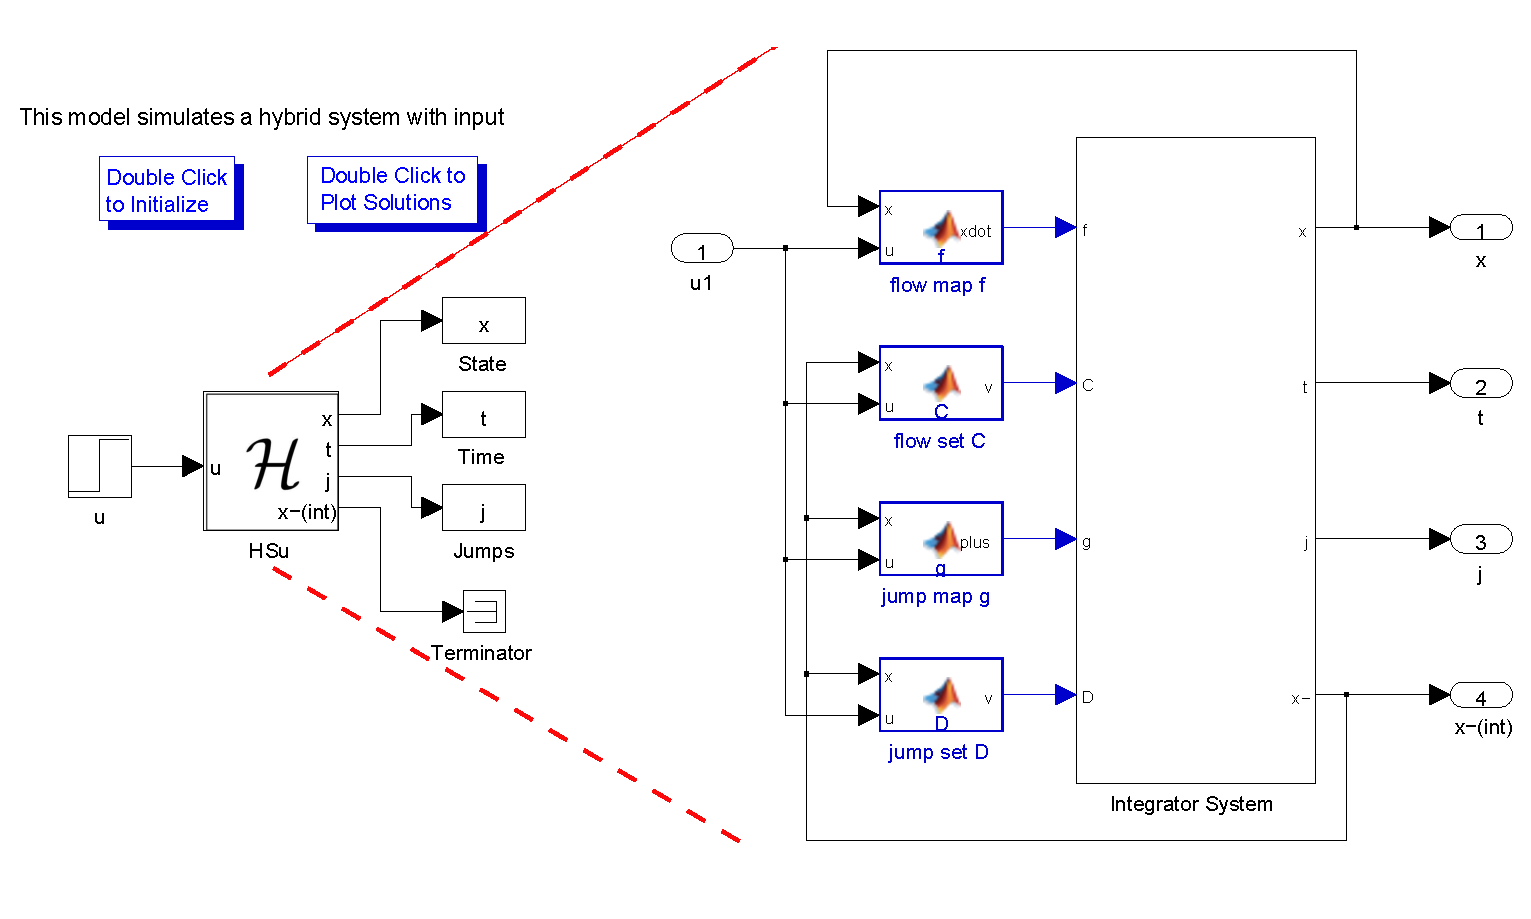
\includegraphics[width=.75\textwidth]{figures/Simulink/HSinput.eps}}
\caption{\matlab{}/Simulink implementation of a hybrid system $\HS =(C,f,D,g)$ with inputs.}
\label{fig:HSinput}
  \end{center}
\end{figure}

Figure~\ref{fig:HSinput} shows a Simulink implementation for simulating 
a hybrid system with inputs using embedded \matlab{} functions. 
In this implementation, four basic blocks are used to define the {\em data} 
of the hybrid system $\HS$:
\begin{itemize}
\item The flow map is implemented in an {\em Embedded \matlab{} function block} 
executing the function {\tt
f.m}. Its input is a vector with components defining the state of the system $x$, and the input $u$.
Its output is the value of the flow map $f$ which is connected to the  input of an integrator.
\item The flow set is implemented in an {\em Embedded \matlab{} function block} 
executing the function {\tt
C.m}. Its input is a vector with components $x^-$ and input $u$ of the {\em Integrator system}. 
Its output is equal to $1$ if the state belongs to the set $C$ or equal to $0$ otherwise.
The minus notation denotes the previous value of the variables (before integration). 
The value $x^-$ is obtained from the state port of the integrator.
\item The jump map is implemented in an {\em Embedded \matlab{} function block} 
executing the function {\tt
g.m}. Its input is a vector with components $x^-$ and input $u$ of the {\em Integrator system}. 
Its output is the value of the jump map $g$.
\item The jump set is implemented in an {\em Embedded \matlab{} function block} 
executing the function {\tt
D.m}. Its input is a vector with components $x^-$ and input $u$ of the {\em Integrator system}. 
Its output is equal to $1$ if the state belongs to $D$ or equal to $0$ otherwise.
\end{itemize}


In our implementation, \matlab{} {\tt .m} files are used. 
The file {\tt initialization.m} is used to define initial variables before simulation. 
The file {\tt postprocessing.m} is used to plot the solutions after a simulation is complete. 
These two {\tt .m} files are called by double-clicking the {\em Double Click to...} 
blocks at the top of the Simulink Model (see Section \ref{sec:postprocessing} 
for more information on these {\tt .m} files and their use).


\subsection{Specialized library for simulation of Cyber-Physical Systems}
\label{sec:CPS}
The HyEQ Toolbox includes a series of blocks that model elements 
of a cyber-physical system (CPS). Those models are special instances 
of the hybrid systems blocks described above, particularly the blocks 
that use embedded \matlab{} functions.
A cyber-physical system is given by the interconnection between a physical process, 
{\em the plant}, a computer algorithm used for control, {\em the controller}; 
and  the subsystems needed to interconnect the plant and the controller, i.e., 
{\em the interfaces,  converters, and signal conditioners}. 
Most of the elements described in this section are presented in an extended form in~\cite{San17}.

In these notes, the temporal evolution of the variables of a cyber-physical system
are captured using dynamical models.
In this document, we advocate that hybrid dynamical system models
can be employed to capture the behavior of cyber-physical systems.
More precisely, the evolution of the continuous variables is captured by 
{\em differential equations}
while the evolution of the discrete variables is captured by
{\em difference equations}.
These equations are typically nonlinear
due to the complexity of the dynamics of those variables.
Furthermore, conditions determining the change of 
the continuous and discrete variables according to the said
equations/inclusions can be conveniently captured by functions of the
variables, inputs, and outputs.  
%In the next sections, these models are introduced in detail and illustrated in examples.
In Figure~\ref{fig:CPS}, cyber and physical blocks are implemented within the HyEQ simulator.

\begin{figure}[ht]
  \begin{center}
    {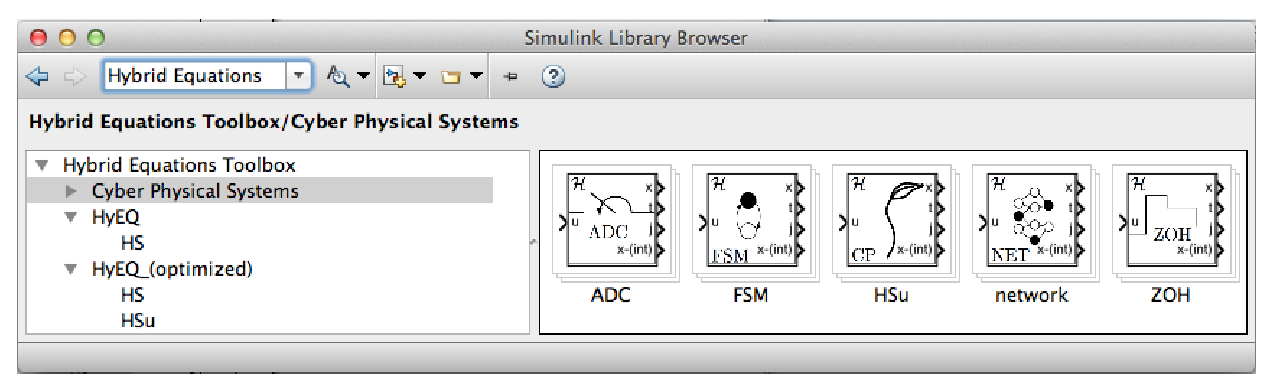
\includegraphics[width=1.0\textwidth]{figures/Simulink/SimulinkimplementationCPS_Mac.eps}}
\caption{\matlab{}/Simulink library blocks for Cyber-Physical Systems implementation.}
\label{fig:CPS}
  \end{center}
\end{figure}

\subsubsection{Models of physical components}
\label{sec:PhysicalModels}
%\subsubsection{Continuous processes}

The physical components of a cyber-physical system include the analog elements, 
physical systems, and the environment. 
Consider a model of a physical system given by a differential equation $\dot{x} = f(x,u)$ 
and a output map $y = h(x,u)$. Among the many possible models available, 
we capture the dynamics of the physical components
by using the hybrid systems framework by
\begin{subequations}\label{eqn:CPSplant}
\begin{align}
\dot{x} &= f(x,u), 
&C &:= \{ x\ |\ x \in \Re^{n}\},\\
\x^+ &= g(x) =\emptyset,
&D &:= \emptyset,\\
y &= h(x,u)
\end{align}
\end{subequations}
Particularly, the model in~\eqref{eqn:CPSplant} can be implemented 
in the simulink block {\em HSu} in Figures~\ref{fig:HSinput}) and~\ref{fig:CPS}).

\subsubsection{Models of cyber components}
\label{sec:CyberModels}

The cyber components of a cyber-physical system 	
include those in charge of performing computations, 
implementing algorithms, and transmitting digital data over networks.
The tasks performed by the code (at the software level) 
and the logic-based mechanisms (at the circuit level)
involve variables that only change at discrete events, not necessarily periodically.

We denote the state
variable of the cyber components by $\xc \in \xcSpace$, where $\xcSpace \subset \reals^{n_C}$ is the state space. 
The dynamics of $\eta$ are defined by a difference equation with
right-hand side defined by the map $\gc$. 
We let $\uc \in \ucSpace \subset \reals^{m_C}$ denote the input signals affecting the cyber components
and $\yc\in\reals^{r_C}$ to be the output defined by
the output function $\hc$, which is a function of the state $\xc$ and
of the input $\uc$. With these definitions, the general mathematical
description of the cyber component is
\begin{eqnarray} \label{eqn:cyber}
\xc^+ = \gc(\xc,\uc), \  \ \yc &=& \hc(\xc,\uc) \qquad 
\end{eqnarray}
In certain cases, it would be needed to impose restrictions on the state and inputs to the cyber component. 
%Such is the case when it is needed
%to determine the values 
%(e.g., the state belongs to a
%manifold or the input is constrained), 
%or to determine conditions that they should satisfy
%so as to evolve continuously according to \eqref{eqn:env}.
Such conditions can be modeled 
imposing that $\xc$ and $\uc$ belong to a subset of their state space,
namely,
\begin{equation}\label{eqn:cyberD}
(\xc,\uc) \in \Dc \subset \xcSpace \times \ucSpace
\end{equation}
The model of the cyber components 
is given by \eqref{eqn:cyber}-\eqref{eqn:cyberD}.
Next, we provide specific constructions of models of cyber components.

\begin{enumerate}
\item[1)] {\em Pure Finite State Machines.}
A finite state machine (FSM) or deterministic finite automaton (DFA) is a system with
inputs, states, and outputs taking values from discrete sets 
that are updated at discrete transitions (or jumps) triggered by its inputs. 
Then, given a FSM and an initial state $\xlogic_0 \in \xlogicSpace$,  
a transition to a state $\xlogic_1 = \delta(\xlogic_0,\uc)$ is performed
when an input $\uc \in \Sigma$ is applied to it.
After the transition, the output of the FSM is updated to $\hc(\xlogic_1)$.
This mechanism can be captured by the difference equation
\begin{eqnarray}\label{eqn:FSMmodel}
  \xlogic^+ & = & \delta(\xlogic,\uc)  \qquad \yc \ 
              = \ \hc(\xlogic) \qquad (\xlogic,\uc) \in \xlogicSpace \times \Sigma
\end{eqnarray}
This model captures the dynamics
the model of the cyber components 
in \eqref{eqn:cyber}-\eqref{eqn:cyberD}
with
$$
  \xc = \xlogic, \qquad \xcSpace = \xlogicSpace, \qquad 
  \ucSpace = \Sigma, \qquad \gc = \delta, \qquad \Dc = \xcSpace\times\ucSpace
$$
Note that there is no notion of time associated with the FSM model above. 
An example of this model is presented in Example~\ref{ex:FSM}.
In addition, the block FSM in Figure~\ref{fig:CPS} can be used to model these type of systems.
\medskip

\item[2)] {\em Analog-to-Digital Converters.}
Analog-to-digital converters (ADCs),  or simply sampling devices,
are commonly used to provide measurements of the physical systems
to the cyber components. Their main
function is to sample their input, which is usually the output of the sensors measuring
the output $\yp$, at a given periodic rate $T^*_s$ and to make these samples
available to the embedded computer. A basic model for a sampling device
consists of a timer state and a sample state.  When the timer reaches
the value of the sampling time $T^*_s$, the timer is reset to zero and
the sample state is updated with the inputs to the sampling device. 

The model for the sampling device we propose
has both continuous and discrete dynamics.
% and
%consequently, it is a hybrid system itself. 
If the timer state has not reached $T^*_s$, then the dynamics are such that the timer state
increases continuously with a constant, unitary rate. When $T^*_s$ is
reached, the timer state is reset to zero and the sample state is
mapped to the inputs of the sampling device. 
To implement this mechanism, we employ a timer state 
$\tau_s \in \realsgeq$ and a sample state $m_s \in \reals^{r_P}$.
The input to the sampling device is denoted by $v_s \in \reals^{r_p}$. 
The model of the sampling devices is
\begin{eqnarray}\label{eqn:ADCmodel-a}
\left.
\begin{array}{l}
\dot{\tau}_s =\ 1,  \ \
\dot{m}_s  =\ 0
\end{array}
\right. & \mbox{ when }& \tau_s \in [0,T^*_s] \\ \label{eqn:ADCmodel-b}
\left.
\begin{array}{l}
\tau_s^+  =\ 0,  \ \
m_s^+ =\ v_s
\end{array}
\right. & \mbox{ when }& \tau_s \geq T^*_s
\end{eqnarray}

In practice,
there exists a time, usually called {\em the ADC acquisition time},
between the triggering of the ADC with the sampling device and the update of its output. Such a
delay limits the number of samples per second 
%(SPS) 
that the ADC can provide. 
Additionally, an ADC can store and process finite-length digital words, which causes quantization. 
The model above omits effects such as acquisition delays
and quantization effects, but those can be incorporated if needed.
In particular, quantization effects can be added to the model 
in \eqref{eqn:ADCmodel-a}-\eqref{eqn:ADCmodel-b}
by replacing the update law for $m_s$ to
$m_s^+ = \mbox{round}(v_s)$, where the function 
$\mbox{round}$ is such that $ \mbox{round}(v_s)$ is the
closest number to $v_s$ that the machine precision can represent.
\medskip

\item[3] {\em Digital-to-Analog Converters.}
The digital signals in the cyber components need to be converted
to analog signals for their use in the physical world.
Digital-to-analog converters (DACs) perform such a task 
by converging digital signals into analog equivalents.
One of the most common models for a DAC
is the zero-order hold model (ZOH). In simple terms, a ZOH converts
a digital signal at its input into an analog signal 
at its output.  
Its output is updated at discrete time instants, typically periodically,
and held constant in between updates, until new information is available at the
next sampling time. We will model DACs as ZOH devices with dynamics
similar to \eqref{eqn:ADCmodel-a}-\eqref{eqn:ADCmodel-b}. Let
$\tau_h\in\realsgeq$ be the timer state, $m_h \in \reals^{r_C}$ be the
sample state (note that the value of $h$ indicates the number of DACs
in the interface), and $v_h \in \reals^{r_C}$ be the inputs of the DAC.
Its operation is as follows. When $\tau_h \leq 0$, the timer state
is reset to $\tau_r$ and the sample state is updated with $v_h$ (usually
the output of the embedded computer), where $\tau_r\in[T^{\mbox{min}},T^{\mbox{max}}]$ 
is a random variable that models the time in-between communication instants and 
$T^{\mbox{min}}\leq T^{\mbox{max}}$. A model that captures this
mechanism is given by 
\begin{eqnarray}\label{eqn:DACmodel-a}
\left.
\begin{array}{l}
\dot{\tau}_h =\ -1,   \ \
\dot{m}_h  =\ 0
\end{array}
\right. & \mbox{ when }& \tau_h \in [T^{\mbox{min}},T^{\mbox{max}}] \\ \label{eqn:DACmodel-b}
\left.
\begin{array}{ll}
\tau_h^+  =\ \tau_r,  \ \
m_h^+ =\ v_h
\end{array}
\right. & \mbox{ when }& \tau_h \leq T^{\mbox{min}}
\end{eqnarray}
\medskip

\item[4] {\em Digital Networks.}
The information transfer between the physical and cyber components, or between 
subsystems within the cyber components, might occur over a digital communication network.  
The communication links bridging each of these components
are not capable of continuously transmitting information, but rather,
they can only transmit sampled (and quantized) information at discrete time instants.
Combining the ideas in the models of the converters in the previous items, 
we propose a model of a  digital network link that has a variable that 
triggers the transfer of information provided at its input, and that
stores that information until new information arrives.
We assume that the transmission of information occurs at instants 
$\{t_i\}_{i=1}^{i^*}$, $i^* \in \nats\cup \{\infty\}$, satisfying
\begin{eqnarray}\non
T^{*\min}_{N} & \leq t_{i+1}-t_i\,\leq T^{*\max}_{N}\qquad \forall i\in \{1,2,\ldots, i^*-1\}
%\\
%0&\leq t_{1}-t_0\,\leq T_2
\end{eqnarray}
where $T^{*\min}_{N}$ and $T^{*\max}_{N}$ are constants satisfying  $$T^{*\min}_{N}, T^{*\max}_{N} \in [0,\infty]$$
and $$T^{*\min}_{N} \leq T^{*\max}_{N}$$ and $i^*$ is the number of transmission events, which might be finite or infinite.
The constant $T^{*\min}_{N}$ determines the minimum possible time in between 
transmissions while the constant $T^{*\max}_{N}$ defines the maximum amount of time elapsed between transmissions.
In this way, a communication channel that allows transmission events at a high rate
would have $T^{*\min}_{N}$ small (zero for infinitely fast transmissions), 
while one with slow data rate would have $T^{*\min}_{N}$ large.
The constant $T^{*\max}_{N}$ determines
how often transmissions may take place.
Note that the constants $T^{*\min}_{N}$ and $T^{*\max}_{N}$ can be
generalized to functions so as to change according to other states or inputs.

At every $t_i$, the information at the input $v_N$ of the
communication link is used to update the internal variable 
$m_N$, which is accessible at the output end of the network
and remains constant between communication events.
This internal variable acts as an information buffer, which
can contain not only the latest piece of information transmitted
but also previously transmitted information.
A record of the number of communication events is logged in the internal variable $j_N$. 
At communication events, the value of $j_N$ gets updated 
and remains constant in-between events. 
A mathematical model capturing the said mechanism is given by
\begin{eqnarray}\label{eqn:DigitalLinkModel-a}
\left.
\begin{array}{l}
\dot{\tau}_N =\ -1,   \ \
\dot{m}_N  =\ 0,   \ \
\dot{j}_N =\ 0
\end{array}
\right. & \mbox{ when }& \tau_N \in [0,T^{*\max}_{N}] \\ 
\label{eqn:DigitalLinkModel-b}
\left.
\begin{array}{ll}
\tau_N^+  \in [T^{*\min}_{N},T^{*\max}_{N}],  \ \
m_N^+ =\ v_N,  \ \
j_N^+ = j_N+1
\end{array}
\right. & \mbox{ when }& \tau_N \leq 0
\end{eqnarray}
Note that the update law for $\tau_N$ at jumps is given in terms of a difference inclusion,
which implies that the new value of $\tau_N$ is taken from the set $[T^{*\min}_{N},T^{*\max}_{N}]$.
The dimension of the states and the input would depend on 
the type of components that connect to and from it, and also the size of data transmitted and buffered.
Similar to the models proposed for conversion, 
the model of the digital link \eqref{eqn:DigitalLinkModel-a}-\eqref{eqn:DigitalLinkModel-b}
does not include delays nor quantization, but such effects can be incorporated if needed.
\medskip


\end{enumerate}

\subsection{The Integrator System}
\label{sec:integratorsystem}
In this section we discuss the internals of the {\em Integrator System} shown in Figure~\ref{fig:integratorsystem}.

\begin{figure}[ht]
  \begin{center}
    {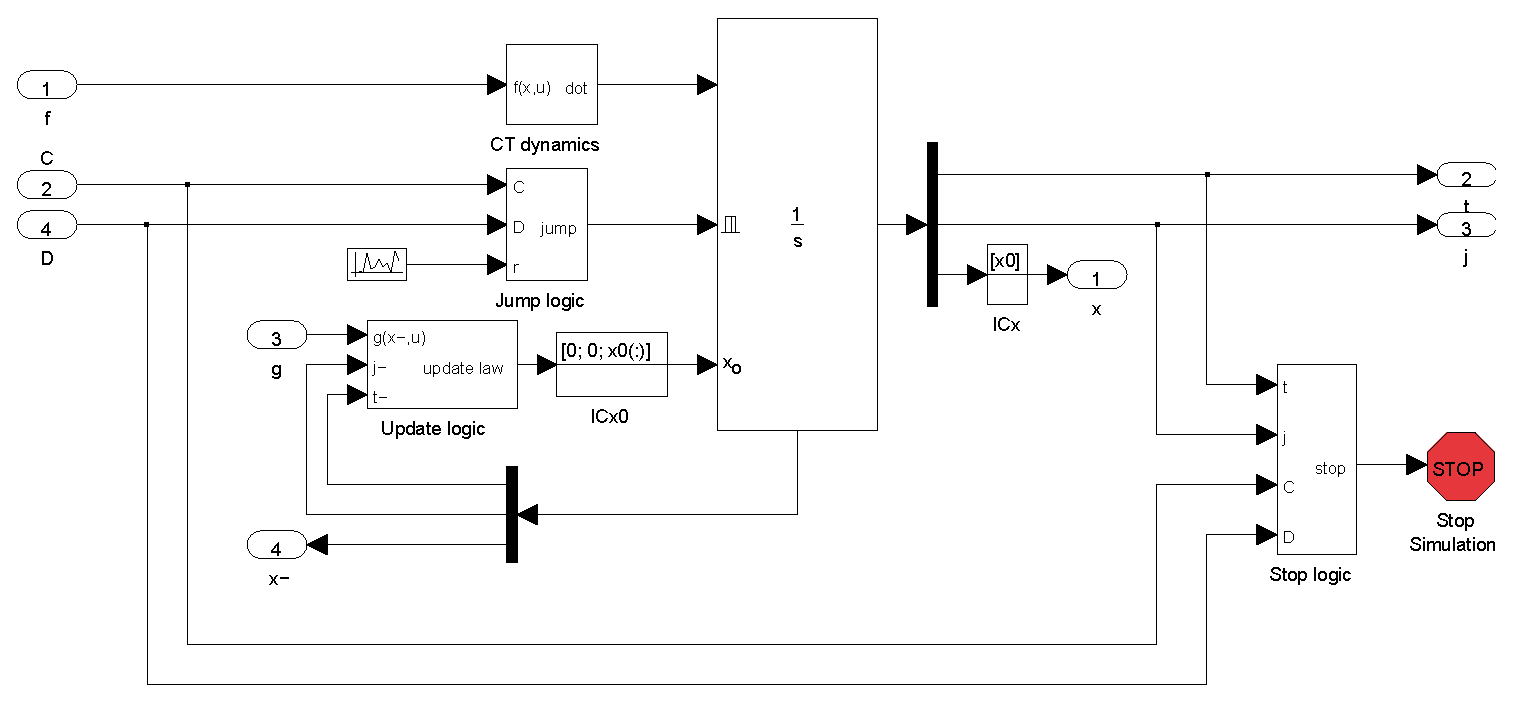
\includegraphics[width=.95\textwidth]{figures/Simulink/Integrator.eps}}
   \caption{Integrator System}
\label{fig:integratorsystem}
  \end{center}
\end{figure}


\subsubsection{Continuous Time (CT) Dynamics}

This block is shown in Figure~\ref{fig:CTdynamics}. 
It defines the continuous-time (CT) dynamics by assembling the 
time derivative of the state $[t\ j\ x^\top]^\top$. 
States $t$ and $j$ are considered states of the system because 
they need to be updated throughout the simulation in order to 
keep track of the time and number of jumps. Without $t$ and $j$, 
solutions could not be plotted accurately.
This is given by
\begin{eqnarray*}
\dot{t} = 1, \qquad \dot{j} = 0, \qquad \dot{x} = f(x,u)\ .
\end{eqnarray*}
Note that input port $1$ takes the value of $f(x,u)$ through the output of the
{\em Embedded \matlab{} function block f} in Figure~\ref{fig:HSinput}.

\begin{figure}[ht]
  \begin{center}
    {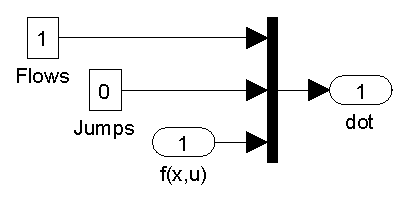
\includegraphics[width=.4\textwidth]{figures/Simulink/CTdynamics.eps}}
   \caption{CT dynamics}
\label{fig:CTdynamics}
 \end{center}
\end{figure}


\subsubsection{Jump Logic}

This block is shown in Figure~\ref{fig:JumpLogic}. 
The inputs to the jump logic block are the output of the blocks {\em C} and {\em D} 
indicating whether the state is in those sets or not, 
and a random signal with uniform distribution in $[0,1]$. 
Figure~\ref{fig:JumpLogic} shows the Simulink blocks used to implement the Jump Logic. 
The variable {\em rule} defines whether the simulator gives priority to jumps, 
priority to flows, or no priority. It is initialized in {\tt initialization.m}.

The output of the Jump Logic is equal to one when:
\begin{itemize}
\item the output of the {\em D block} is equal to one and $rule=1$,
\item the output of the {\em C block} is equal to zero, 
      the output of the {\em D block} is equal to one, and $rule=2$,
\item the output of the {\em C block} is equal to zero, 
      the output of the {\em D block} is equal to one, and $rule=3$,
\item or the output of the {\em C block} is equal to one, 
      the output of the {\em D block} is equal to one, $rule = 3$, 
      and the random signal $r$ is larger or equal than $0.5$.
\end{itemize}
Under these events, the output of this block, which is connected to the integrator external 
reset input, triggers a reset of the integrator, that is, a jump of $\HS$. 
The reset or jump is activated since the configuration of the reset input is set 
to ``level hold'', which executes resets when this external input is equal to one 
(if the next input remains set to one, multiple resets would be triggered). 
Otherwise, the output is equal to zero.

\begin{figure}[ht]
  \begin{center}
    {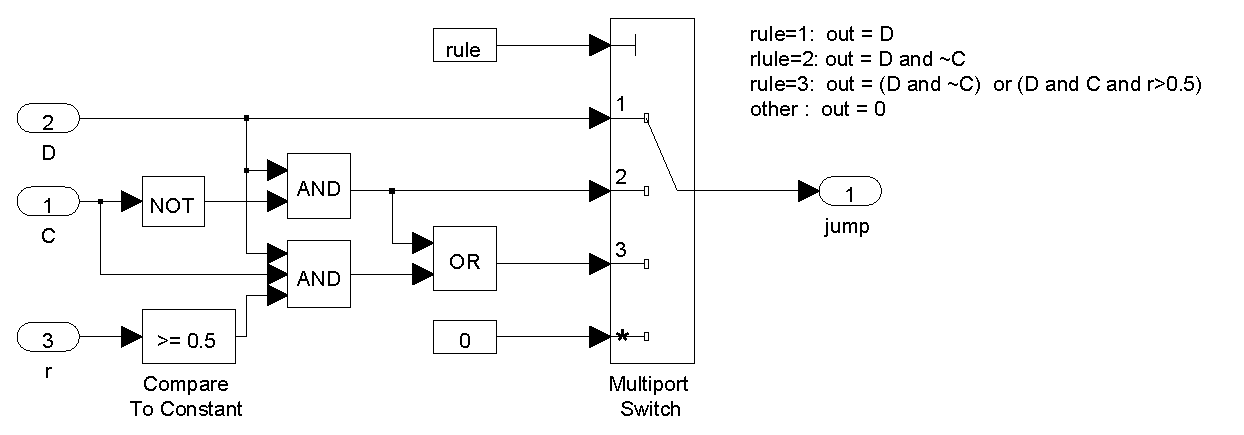
\includegraphics[width=.8\textwidth]{figures/Simulink/JumpLogic.eps}}
   \caption{Jump Logic}
\label{fig:JumpLogic}
  \end{center}
\end{figure}


\subsubsection{Update Logic}

This block is shown in Figure~\ref{fig:UpdateLogic}. 
The update logic uses the {\em state port} information of the integrator. 
This port reports the value of the state of the integrator, $[t\ j\ x^\top]^\top$, 
at the exact instant that the reset condition becomes true. 
Notice that $x^-$ differs from $x$ since at a jump, 
$x^-$ indicates the value of the state that triggers the jump, 
but it is never assigned as the output of the integrator. 
In other words, ``$x \in D$" is checked using $x^-$ and if true, 
$x$ is reset to $g(x^-,u)$. Notice, however, that $u$ is the same because at a jump, 
$u$ indicates the next evaluated value of the input, 
and it is assigned as the output of the integrator. 
The flow time $t$ is kept constant at jumps and $j$ is incremented by one. 
More precisely
\begin{eqnarray*}
t^+=t^-, \qquad j^+=j^-+1,\qquad x^+=g(x^-,u)
\end{eqnarray*}
where $[t^-\ j^-\ {x^-}^\top]^\top$ is the state that triggers the jump.

\begin{figure}[ht]
  \begin{center}
    {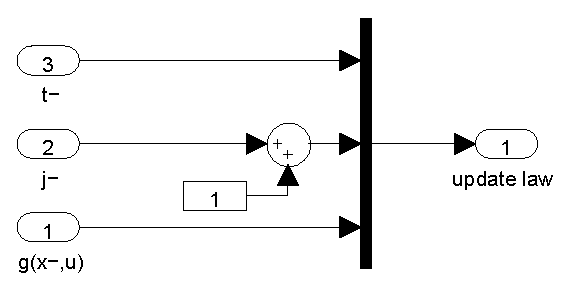
\includegraphics[width=.4\textwidth]{figures/Simulink/UpdateLogic.eps}}
   \caption{Update Logic}
\label{fig:UpdateLogic}
  \end{center}
\end{figure}




\subsubsection{Stop Logic}

This block is shown in Figure~\ref{fig:StopLogic}. 
It stops the simulation under any of the
following events:
\begin{itemize}
\item The flow time is larger than or equal to the maximum flow time specified by $T$.
\item The jump time is larger than or equal to the maximum number of jumps specified by $J$.
\item The state of the hybrid system $x$ is neither in $C$ nor in $D$.
\end{itemize}
Under any of these events, the output of the logic operator
connected to the {\em Stop block} becomes one, stopping the simulation.
Note that the inputs $C$ and $D$ are routed from the output of the blocks 
computing whether the state is in $C$ or $D$ and use the value of $x^-$.

\begin{figure}[ht]
  \begin{center}
    {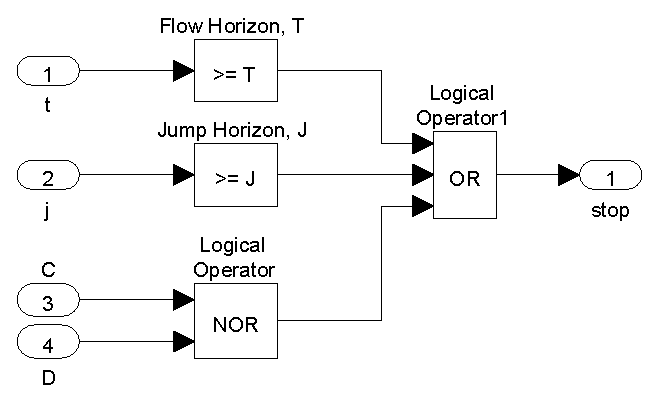
\includegraphics[width=.5\textwidth]{figures/Simulink/StopLogic.eps}}
   \caption{Stop Logic}
\label{fig:StopLogic}
  \end{center}
\end{figure}

%
%\section{Configuration, Initialization, and Postprocessing}
%\label{sec:configinitpost}

\subsection{Software Requirements}
In order to run simulations of single hybrid systems using externally defined functions, 
\matlab{} with Simulink is required.

In order to run simulations using the HyEQ Simulator with embedded \matlab{} functions, 
\matlab{}/Simulink and a supported ANSI, C, or C++ 32-bit compiler must be installed. 
We now briefly describe how to install necessary compilers for Windows and Mac/Linux. 
For more information on supported compilers, please visit 
\url{http://www.mathworks.com/support/compilers/R2012b/win64.html}.


\subsubsection{Configuration of HyEQ Simulator with embedded functions for Windows}
For 32-bit Windows, the LCC compiler is included with \matlab{}. 
First, open \matlab{} and then locate and choose a compiler for 
building MEX-files by typing \begin{verbatim} >> mex -setup \end{verbatim}
into the \matlab{} command window. Then, follow the prompts as shown below.

\begin{verbatim}
>> mex -setup

Welcome to mex -setup.  This utility will help you set up
a default compiler.  For a list of supported compilers, see
http://www.mathworks.com/support/compilers/R2012a/win32.html

Please choose your compiler for building MEX-files:

Would you like mex to locate installed compilers [y]/n? y

Select a compiler:
[1] Lcc-win32 C 2.4.1

[0] None

Compiler: 1

Please verify your choices:

Compiler: Lcc-win32 C 2.4.1

Are these correct [y]/n? y

Done . . .
\end{verbatim}

For 64-bit Windows, a C-compiler is not supplied with \matlab{} ({\color{red} Is this still true?}). 
Before running the HyEQ Toolbox in \matlab{}/Simulink, please follow the following steps:

\begin{enumerate}
\item If you don't have {\em Microsoft .NET Framework 4} on your computer, 
download and install it from
\url{http://www.microsoft.com/en-us/download/details.aspx?id=17851}.
\item Then download and install {\em Microsoft Windows SDK} from
\url{http://www.microsoft.com/en-us/download/details.aspx?id=8279}.
\item Then perform the steps outlined above for 32-bit Windows to 
setup and install the compiler.
\end{enumerate}

As of October 10, 2013, when installing the toolbox in Windows 8, 
please follow the next steps.
\begin{enumerate}
\item If you don't have {\em Microsoft .NET Framework 4} on your computer, 
download and install it from
\url{http://www.microsoft.com/en-us/download/details.aspx?id=8279}.
\item Then download and install {\em Microsoft Windows SDK}
	\begin{itemize}
	\item If you don't have {\em Visual C++ 2010 SP1} installed on your computer:
		\begin{itemize} 
		\item Download and install {\em Microsoft Windows SDK 7.1} from
		\url{http://www.microsoft.com/en-us/download/details.aspx?displaylang=en&id=4422}
		\item Apply the following patch from {\em Microsoft} onto the {\em SDK 7.1} installation: 
          \url{http://www.microsoft.com/en-us/download/details.aspx?displaylang=en&id=4422}
		\end{itemize}
	\item If you have Visual {\em Visual C++ 2010 SP1} or its redistributable packages 
        installed on your computer:
		\begin{itemize}
		\item Uninstall the {\em Visual C++ 2010} redistributable packages, 
          both x64 and x86 versions. This can be done from 
          {\em Control Panel $/$ Uninstall Programs Menu}.
		\item Download and install {\em Microsoft Windows SDK 7.1} from
		      \url{http://www.microsoft.com/en-us/download/details.aspx?displaylang=en&id=4422}
		\item Apply the following patch from {\em Microsoft} onto the {\em SDK 7.1} installation: 
          \url{http://www.microsoft.com/en-us/download/details.aspx?displaylang=en&id=4422}	
		\item Reinstall the {\em Visual C++ 2010} redistributable packages:	
		
		x86 version:
		\url{http://www.microsoft.com/en-us/download/details.aspx?id=5555}
		
		x64 version:
		\url{http://www.microsoft.com/en-us/download/details.aspx?id=14632}
		\end{itemize}
	\end{itemize}
\item Then perform the steps outlined above for 32-bit Windows to 
      setup and install the compiler.
\end{enumerate}

\subsubsection{Configuration of HyEQ Simulator with embedded functions for Mac/Linux}

From a terminal window, check that the file {\tt gcc} is in
the folder {\tt/usr/bin}.
If it is not there, make a symbolic link. 
You might require to install the latest version of {\tt Xcode} first.
In order to generate a symbolic link for gcc, 
that \matlab{} can find to compile the simulation files 
(see \url{http://www.mathworks.com/support/sysreq/previous_releases.html}), 
change folder to {\tt /usr/bin} and then
\begin{verbatim}
sudo ln -s gcc gcc-4.2
\end{verbatim}
\noindent Then, it should be possible to setup the gcc compiler in matlab as follows:

\begin{verbatim}
>> mex -setup
    Options files control which compiler to use, the compiler and link command
    options, and the runtime libraries to link against.

    Using the 'mexsh -setup' command selects an options file that is
    placed in ~/.matlab/R2013b and used by default for 'mexsh'. An options 
    file in the current working directory or specified on the command line 
    overrides the default options file in ~/.matlab/R2013b.
 
    To override the default options file, use the 'mexsh -f' command
    (see 'mexsh -help' for more information).

\end{verbatim}

The options files available for MEX are:

\begin{verbatim}
The options files available for mexsh are:

  1: /Applications/MATLAB_R2013b.app/bin/mexopts.sh : 
      Template Options file for building MEX-files
 
  0: Exit with no changes

Enter the number of the compiler (0-1): 1

Overwrite ~/.matlab/R2013b/mexopts.sh ([y]/n)?: Y

/Applications/MATLAB_R2013b.app/bin/mexopts.sh is being copied to 
/SOME_FOLDER/mexopts.sh

\end{verbatim}

At this point, it is possible to check if the $gcc$ is properly setup by 
testing any of the Simulink examples with embedded functions 
(see Figure~\ref{fig:Simulinklibblocks}) (e.g., 
Examples~\ref{ex:bbinput},~\ref{ex:bbblocks},~\ref{ex:dubinspath},~\ref{ex:interconnection1},~\ref{ex:fireflies} or~\ref{ex:overlap1}).

If an error regarding ``$gmake$'' similar to ``No supported compiler or SDK was found'' 
and/or a warning ``no such sysrooot directory: 
$'$Developer/SDKs/MacOSX10.X.sdk$'$'' is shown when compiling, 
please consider the following procedure.

\begin{itemize}
\item[A.] For Matlab 2013b and previous:

The compiler can not find the appropriate path. It is necessary to change some lines in the 
file ``$mexopts.sh$'' (copied previously in the folder ``SOME\_FOLDER'') .

First, locate the Xcode-SDK in your hard drive. 
Open a terminal window and execute the following command
\begin{verbatim}
xcodebuild -version -sdk macosx10.9 Path
\end{verbatim}
which returns the location of MacOSX10.9.sdk, denoted here as SDK\_FOLDER. 
Now, in the \matlab{} command window locate the file ``$mexopts.sh$'' by typing 
\begin{verbatim}
cd /SOME_FOLDER/
\end{verbatim}
Then, open the file 
\begin{verbatim}
edit mexopts.sh
\end{verbatim}
and edit the lines
\begin{itemize}
\item
\begin{verbatim}
SDKROOT='/Developer/SDKs/MacOSX10.X.sdk'
\end{verbatim}
to 
\begin{verbatim}
SDKROOT='SDK_FOLDER'
\end{verbatim}
and
\item
\begin{verbatim}
MACOSX_DEPLOYMENT_TARGET='10.X'
\end{verbatim}
to 
\begin{verbatim}
MACOSX_DEPLOYMENT_TARGET='10.9'
\end{verbatim}
\end{itemize}

Now, it is possible to test if the compiler works. If the following error appears
``\verb!unknown type name 'char16_t'!,'' 
some flags must be changed to avoid this problem. 
It is required to add \verb!-Dchar16_t=UINT16_T! 
and \verb!-std=c++11! to the flags CFLAGS and CFLAGS respectively, e.g., change
\begin{itemize}
\item
\begin{verbatim}
CFLAGS="-fno-common -no-cpp-precomp -arch $ARCHS -isysroot $SDKROOT 
-mmacosx-version-min=$MACOSX_DEPLOYMENT_TARGET"
\end{verbatim}
to
\begin{verbatim}
CFLAGS="-fno-common -no-cpp-precomp -arch $ARCHS -isysroot $SDKROOT 
-mmacosx-version-min=$MACOSX_DEPLOYMENT_TARGET -Dchar16_t=UINT16_T"
\end{verbatim}
and
\item
\begin{verbatim}
CXXFLAGS="-fno-common -no-cpp-precomp -fexceptions -arch $ARCHS -isysroot $SDKROOT 
-mmacosx-version-min=$MACOSX_DEPLOYMENT_TARGET"
\end{verbatim}
to
\begin{verbatim}
CXXFLAGS="-fno-common -no-cpp-precomp -fexceptions -arch $ARCHS -isysroot $SDKROOT 
-mmacosx-version-min=$MACOSX_DEPLOYMENT_TARGET -std=c++11"
\end{verbatim}
\end{itemize}
Finally, restart matlab and test any of the aforementioned Simulink examples.
for more information visit 
{\footnotesize\url{http://www.mathworks.com/matlabcentral/answers/121315-how-to-set-the-c-compiler-of-matlab2013a-in-osx-10-9}}

%---------------------------------
\item[B.] For Matlab 2014b and newer. 

First, locate the Xcode-SDK in your hard drive. 
It may be SDK 10.9, 10.10, 10.11, here we are going to denote it as \textbf{10.X}. 
Open a terminal window and execute the following command
\begin{verbatim}
xcodebuild -version -sdk macosx10.X Path
\end{verbatim}
which returns the location of MacOSX10.X.sdk. 
We are interested in the last portion of the path, 
specifically after /Applications/Xcode.app/.Contents/Developer/, 
denoted here as \textbf{SDK\_FOLDER}. Now, locate and edit the following files
\begin{verbatim}/Applications/MATLAB_R201??.app/bin/maci64/mexopts/clang_maci64.xml\end{verbatim}
\begin{verbatim}/Applications/MATLAB_R201??.app/bin/maci64/mexopts/clang++_maci64.xml\end{verbatim}
Inside those files there are the lines
\begin{verbatim}
<dirExists name="$$/Platforms/MacOSX.platform/Developer/SDKs/MacOSX10.10.sdk" />
<cmdReturns name="find $$ -name MacOSX10.10.sdk" />
\end{verbatim}

edit (or add below those lines) the lines
\begin{itemize}
\item
\begin{verbatim}
<dirExists name="$$SDK\_FOLDER" />
\end{verbatim}
and
\item
\begin{verbatim}
<cmdReturns name="find $$ -name MacOSX10.X.sdk" />
\end{verbatim}
\end{itemize}

Finally, restart \matlab{} and test any of the aforementioned Simulink examples.
For more information visit 
{\footnotesize\url{https://bitbucket.org/d2d-development/d2d-software/issues/46/xcode-7-on-osx-with-matlab-r2015a-b}}
\end{itemize}


\subsection{Configuration of Integration Scheme}
Before a simulation is started, it is important to determine the needed integrator scheme, 
zero-cross detection settings, precision, and other tolerances. 
Using the default settings does not always give the most 
efficient or most accurate simulations. 
One way to edit these settings is to open the Simulink Model, 
select {\tt Simulation>Configuration Parameters>Solver}, 
and change the settings there. We have made this simple by defining variables 
for configuration parameters in the {\tt initialization.m} file. 
The last few lines of the {\tt initialization.m} file look like that given below.\\

\code{config\_inst.m}
% % This file was automatically created from the m-file 
% "m2tex.m" written by USL. 
% The fontencoding in this file is UTF-8. 
%  
% You will need to include the following two packages in 
% your LaTeX-Main-File. 
%  
% \usepackage{color} 
% \usepackage{fancyvrb} 
%  
% It is advised to use the following option for Inputenc 
% \usepackage[utf8]{inputenc} 
%  
  
% definition of matlab colors: 
\definecolor{mblue}{rgb}{0,0,1} 
\definecolor{mgreen}{rgb}{0.13333,0.5451,0.13333} 
\definecolor{mred}{rgb}{0.62745,0.12549,0.94118} 
\definecolor{mgrey}{rgb}{0.5,0.5,0.5} 
\definecolor{mdarkgrey}{rgb}{0.25,0.25,0.25} 
  
\DefineShortVerb[fontfamily=courier,fontseries=m]{\$} 
\DefineShortVerb[fontfamily=courier,fontseries=b]{\#} 
  
\begin{Verbatim}[commandchars=\$\{\},numbers=left,numbersep=2pt] 

    $textcolor{mgreen}{%configuration of solver} 
    RelTol = 1e-8; 
    MaxStep = .001;  
\end{Verbatim}  
  
\UndefineShortVerb{\$} 
\UndefineShortVerb{\#} 
 
\label{scr:config_inst}

In these lines, ``RelTol = 1e-8" and ``MaxStep = .001" define the relative tolerance 
and maximum step size of the ODE solver, respectively. 
These parameters greatly affect the speed and accuracy of solutions.

\subsection{Initialization}

When the block labeled {\em Double Click to Initialize} at the top of the 
Simulink Model is double-clicked, the simulation variables are initialized 
by calling the script {\tt initialization.m}. 
The script {\tt initialization.m} defines the initial conditions by defining 
the initial values of the state components, any necessary parameters, 
the maximum flow time specified by $T$, the maximum number of jumps specified by $J$, 
and tolerances used when simulating. 
These can be changed by editing the script file {\tt initialization.m}. 
See below for sample code to initialize the bouncing ball example, 
Example~\ref{ex:bbinput}.\\

\code{initializationBB\_inst.m}
% % This file was automatically created from the m-file 
% "m2tex.m" written by USL. 
% The fontencoding in this file is UTF-8. 
%  
% You will need to include the following two packages in 
% your LaTeX-Main-File. 
%  
% \usepackage{color} 
% \usepackage{fancyvrb} 
%  
% It is advised to use the following option for Inputenc 
% \usepackage[utf8]{inputenc} 
%  
  
% definition of matlab colors: 
\definecolor{mblue}{rgb}{0,0,1} 
\definecolor{mgreen}{rgb}{0.13333,0.5451,0.13333} 
\definecolor{mred}{rgb}{0.62745,0.12549,0.94118} 
\definecolor{mgrey}{rgb}{0.5,0.5,0.5} 
\definecolor{mdarkgrey}{rgb}{0.25,0.25,0.25} 
  
\DefineShortVerb[fontfamily=courier,fontseries=m]{\$} 
\DefineShortVerb[fontfamily=courier,fontseries=b]{\#} 
  
\noindent              
 \hspace*{-1.6em}{\scriptsize 1}$  $\color{mgreen}$% initialization for bouncing ball example$\color{black}$$\\
 \hspace*{-1.6em}{\scriptsize 2}$  clear $\color{mred}$all$\color{black}$$\\
 \hspace*{-1.6em}{\scriptsize 3}$  $\color{mgreen}$% initial conditions$\color{black}$$\\
 \hspace*{-1.6em}{\scriptsize 4}$  x0 = [1;0];$\\
 \hspace*{-1.6em}{\scriptsize 5}$  $\color{mgreen}$% simulation horizon$\color{black}$$\\
 \hspace*{-1.6em}{\scriptsize 6}$  T = 10;$\\
 \hspace*{-1.6em}{\scriptsize 7}$  J = 20;$\\
 \hspace*{-1.6em}{\scriptsize 8}$  $\color{mgreen}$% rule for jumps$\color{black}$$\\
 \hspace*{-1.6em}{\scriptsize 9}$  $\color{mgreen}$% rule = 1 -> priority for jumps$\color{black}$$\\
 \hspace*{-2em}{\scriptsize 10}$  $\color{mgreen}$% rule = 2 -> priority for flows$\color{black}$$\\
 \hspace*{-2em}{\scriptsize 11}$  $\color{mgreen}$% rule = 3 -> no priority, random selection when simultaneous conditions$\color{black}$$\\
 \hspace*{-2em}{\scriptsize 12}$  rule = 1;$\\
 \hspace*{-2em}{\scriptsize 13}$  $\color{mgreen}$%configuration of solver$\color{black}$$\\
 \hspace*{-2em}{\scriptsize 14}$  RelTol = 1e-8;$\\ 
  
\UndefineShortVerb{\$} 
\UndefineShortVerb{\#}
\label{scr:initializationBB_inst}

It is important to note that variables called in the 
{\em Embedded \matlab{} function blocks}
must be added as inputs and labeled as ``parameters". 
This can be done by opening the {\em Embedded \matlab{} function block}
selecting {\tt Tools>Edit Data/Ports} and setting the scope to {\tt
Parameter}.

After the block labeled {\em Double Click to Initialize} is double-clicked 
and the variables initialized, the simulation is run by clicking the run button 
or selecting {\tt Simulation>Start}.


\subsection{Postprocessing and Plotting solutions}
\label{sec:postprocessing}

A similar procedure is used to define the plots of solutions after the simulation is run. 
The solutions can be plotted by double-clicking on the block at the top of the Simulink Model 
labeled {\em Double Click to Plot Solutions} which calls the script {\tt postprocessing.m}. 
The script {\tt postprocessing.m} may be edited to include the desired postprocessing and solution plots. 
See below for sample code to plot solutions to the bouncing ball example, Example~\ref{ex:bbinput}. 
The functions used to generate the plots are described in Section~\ref{sec:plotfcn}.\\

\code{postprocesingBB\_inst.m}
% % This file was automatically created from the m-file 
% "m2tex.m" written by USL. 
% The fontencoding in this file is UTF-8. 
%  
% You will need to include the following two packages in 
% your LaTeX-Main-File. 
%  
% \usepackage{color} 
% \usepackage{fancyvrb} 
%  
% It is advised to use the following option for Inputenc 
% \usepackage[utf8]{inputenc} 
%  
  
% definition of matlab colors: 
\definecolor{mblue}{rgb}{0,0,1} 
\definecolor{mgreen}{rgb}{0.13333,0.5451,0.13333} 
\definecolor{mred}{rgb}{0.62745,0.12549,0.94118} 
\definecolor{mgrey}{rgb}{0.5,0.5,0.5} 
\definecolor{mdarkgrey}{rgb}{0.25,0.25,0.25} 
  
\DefineShortVerb[fontfamily=courier,fontseries=m]{\$} 
\DefineShortVerb[fontfamily=courier,fontseries=b]{\#} 
  
\noindent                  
 \hspace*{-1.6em}{\scriptsize 1}$  $\color{mgreen}$%postprocessing for the bouncing ball example$\color{black}$$\\
 \hspace*{-1.6em}{\scriptsize 2}$  $\color{mgreen}$% plot solution$\color{black}$$\\
 \hspace*{-1.6em}{\scriptsize 3}$  figure(1)$\\
 \hspace*{-1.6em}{\scriptsize 4}$  clf$\\
 \hspace*{-1.6em}{\scriptsize 5}$  subplot(2,1,1),plotflows(t,j,x)$\\
 \hspace*{-1.6em}{\scriptsize 6}$  grid $\color{mred}$on$\color{black}$$\\
 \hspace*{-1.6em}{\scriptsize 7}$  ylabel($\color{mred}$'x'$\color{black}$)$\\
 \hspace*{-1.6em}{\scriptsize 8}$  subplot(2,1,2),plotjumps(t,j,x)$\\
 \hspace*{-1.6em}{\scriptsize 9}$  grid $\color{mred}$on$\color{black}$$\\
 \hspace*{-2em}{\scriptsize 10}$  ylabel($\color{mred}$'x'$\color{black}$)$\\
 \hspace*{-2em}{\scriptsize 11}$  $\color{mgreen}$% plot hybrid arc$\color{black}$$\\
 \hspace*{-2em}{\scriptsize 12}$  figure(2)$\\
 \hspace*{-2em}{\scriptsize 13}$  plotHybridArc(t,j,x)$\\
 \hspace*{-2em}{\scriptsize 14}$  xlabel($\color{mred}$'j'$\color{black}$)$\\
 \hspace*{-2em}{\scriptsize 15}$  ylabel($\color{mred}$'t'$\color{black}$)$\\
 \hspace*{-2em}{\scriptsize 16}$  zlabel($\color{mred}$'x'$\color{black}$)$\\
 \hspace*{-2em}{\scriptsize 17}$  grid $\color{mred}$on$\color{black}$$\\
 \hspace*{-2em}{\scriptsize 18}$  view(37.5,30)$\\ 
  
\UndefineShortVerb{\$} 
\UndefineShortVerb{\#}
\label{scr:postprocesingBB_inst}


%In the \matlab{}-based HyEQ Simulator, solutions are plotted by calling these 
% functions at the end of the {\tt run.m} function.

% \section{Examples}
% \label{sec:examples}

% The examples below illustrate the use of the Simulink implementation above.

\begin{example}{bouncing ball with input}
\label{ex:bbinput} For the simulation of the bouncing ball system  with a constant input and regular data given by

\begin{eqnarray}
f(x,u):=\left[
 \begin{array}{c}
   x_{2} \\
 -\gamma
 \end{array}
\right],
   C : = \defset{ (x,u) \in \Re^{2}\times\Re}{x_{1} \geq u} \\
g(x,u):=\left[ \begin{array}{c}
 u \\
- \lambda x_{2}
\end{array}
\right]\ ,
    D: = \defset{ (x,u) \in \Re^{2}\times\Re}{x_{1} \leq u \ , \
  x_{2} \leq 0}
\end{eqnarray}
where $\gamma >0$ is the gravity constant, $u$ is the input constant,
and $\lambda \in [0,1)$ is the restitution coefficient.
The MATLAB scripts in each of the function blocks of the implementation above are given as follows.
An input was chosen to be $u(t,j) = 0.2$ for all $(t,j)$. The constants for the bouncing ball
system are $\gamma = 9.81$ and $\lambda=0.8$.

\bigskip

\noindent The following procedure is used to simulate this example using the model in the file {\tt Example\_1\_2a.slx}:
\begin{itemize}
\item {\tt Example\_1\_2a.slx} is opened in MATLAB/Simulink.
\item The {\em Embedded MATLAB function blocks} {\em f, C, g, D} are edited by double-clicking on the block and editing the script. In each embedded function block, parameters must be added as inputs and defined as parameters by selecting {\tt Tools>Edit Data/Ports}, and setting the scope to {\tt Parameter}. For this example, {\em gamma} and {\em lambda} are defined in this way.
\item The initialization script {\tt initialization.m} is edited by opening the file and editing the script. The flow time and jump horizons, $T$ and $J$ are defined as well as the initial conditions for the state vector, $x_0$, and input vector, $u_0$, and a rule for jumps, $rule$.
\item The postprocessing script {\tt postprocessing.m} is edited by opening the file and editing the script. Flows and jumps may be plotted by calling the functions {\em plotflows} and {\em plotjumps}, respectively. The hybrid arc may be plotted by calling the function {\em plotHybridArc}.
\item The simulation stop time and other simulation parameters are set to the values defined in {\tt initialization.m} by selecting {\tt Simulation>Configuration Parameters>Solver} and inputting $T$, $RelTol$, $MaxStep$, etc..
\item The masked integrator system is double-clicked and the simulation horizons and initial conditions are set as desired.
\item The block labeled {\em Double Click to Initialize} is double-clicked to initialize variables.
\item The simulation is run by clicking the run button or selecting {\tt Simulation>Start}.
\item The block labeled {\em Double Click to Plot Solutions} is double-clicked to plot the desired solutions.
\end{itemize}

%\begin{figure}[ht]
%  \begin{center}
%  \psfrag{flows [t]}[c]{flows [$t$]}
%  \psfrag{jumps [j]}[c]{jumps [$j$]}
%  \psfrag{x1}[c]{$x_1$}
%    {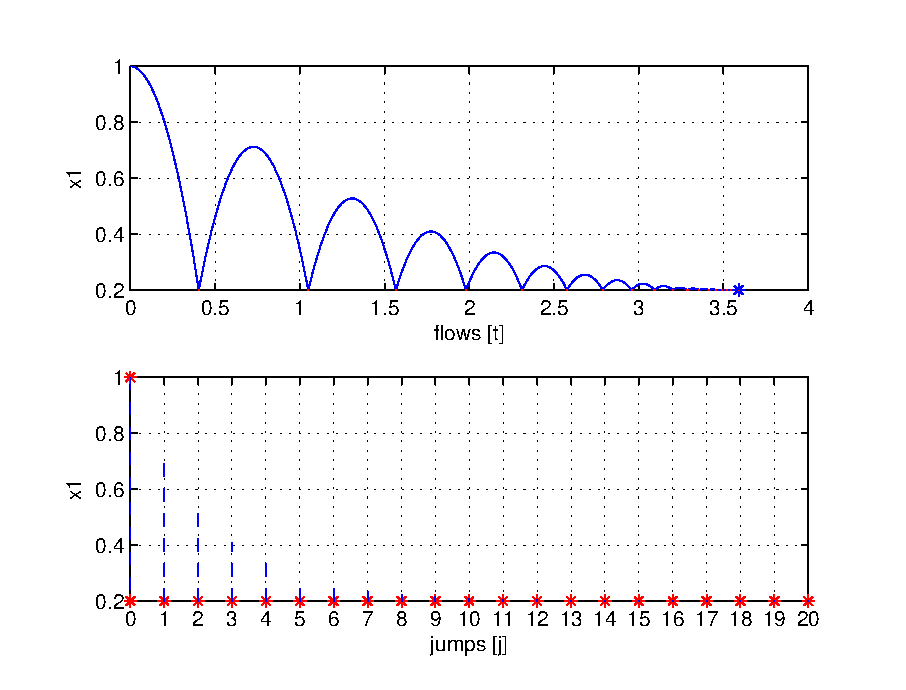
\includegraphics[width=.8\textwidth]{figures/Examples/FlowsAndJumps1.eps}}
%   \caption{Solution of Example~\ref{ex:bbinput}: height}
%\label{fig:input-1}
%  \end{center}
%\end{figure}
%
%\begin{figure}[ht]
%  \begin{center}
%  \psfrag{flows [t]}[c]{flows [$t$]}
%  \psfrag{jumps [j]}[c]{jumps [$j$]}
%  \psfrag{x2}[c]{$x_2$}
%    {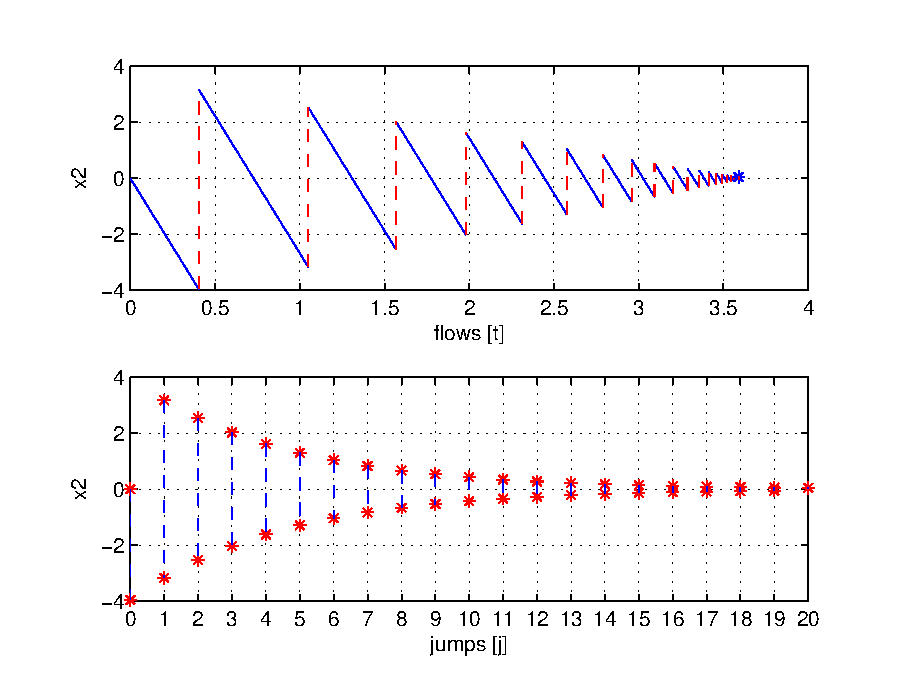
\includegraphics[width=.8\textwidth]{figures/Examples/FlowsAndJumps2.eps}}
%   \caption{Solution of Example~\ref{ex:bbinput}: velocity}
%\label{fig:input-2}
%  \end{center}
%\end{figure}

\begin{figure}[ht]
\begin{center}
\subfigure[Height \label{fig:input-1}]
{
\psfragfig[width=.45\textwidth]{figures/Examples/FlowsAndJumps1}
{
  \psfrag{flows [t]}[c]{flows [$t$]}
  \psfrag{jumps [j]}[c]{jumps [$j$]}
  \psfrag{x1}[c]{$x_1$}
  \psfrag{x2}[c]{$x_2$}
}
}
\qquad
\subfigure[Velocity \label{fig:input-2}]
{
    \psfragfig[width=.45\textwidth]{figures/Examples/FlowsAndJumps2}
{
  \psfrag{flows [t]}[c]{flows [$t$]}
  \psfrag{jumps [j]}[c]{jumps [$j$]}
  \psfrag{x1}[c]{$x_1$}
  \psfrag{x2}[c]{$x_2$}
}
}
\end{center}
\caption{Solution of Example~\ref{ex:bbinput}}
\end{figure}

\begin{figure}[ht]
  \begin{center}
  \psfrag{t}[c]{$t$}
  \psfrag{j}[c]{$j$}
  \psfrag{x1}[c]{$x_1$}
    {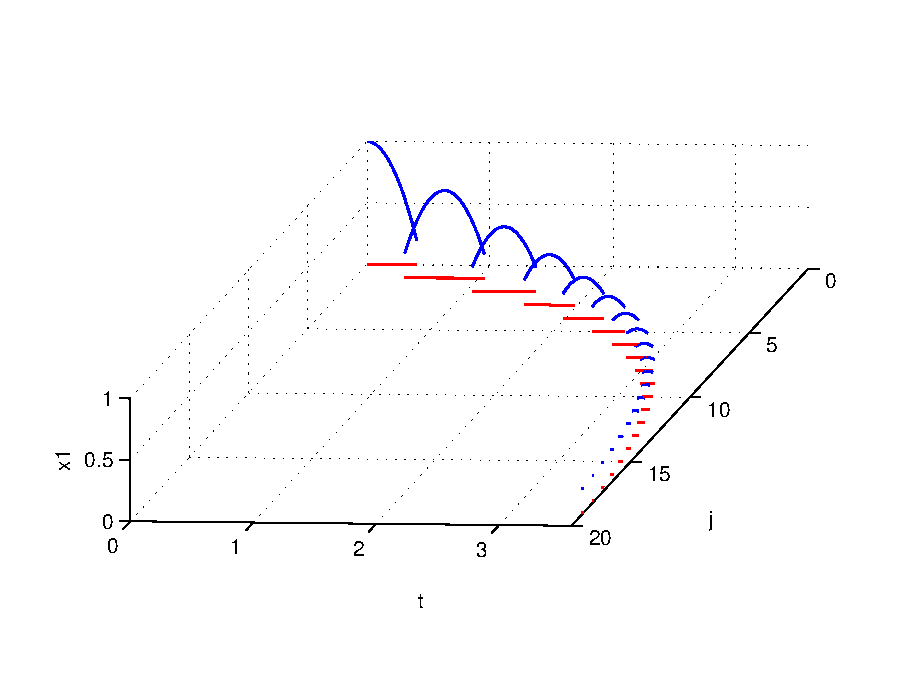
\includegraphics[width=.8\textwidth]{figures/Examples/HybridArc1.eps}}
   \caption{Hybrid arc corresponding to a solution of Example~\ref{ex:bbinput}: height}
  \end{center}
\end{figure}

% Set the location for MATLAB files included via the "\code" command.
\codeLocation{Matlab2tex_1_3}

\code{f.m}
\code{C.m}
\code{g.m}
\code{D.m}

% Flow map
% %\scriptsize
% % This file was automatically created from the m-file 
% "m2tex.m" written by USL. 
% The fontencoding in this file is UTF-8. 
%  
% You will need to include the following two packages in 
% your LaTeX-Main-File. 
%  
% \usepackage{color} 
% \usepackage{fancyvrb} 
%  
% It is advised to use the following option for Inputenc 
% \usepackage[utf8]{inputenc} 
%  
  
% definition of matlab colors: 
\definecolor{mblue}{rgb}{0,0,1} 
\definecolor{mgreen}{rgb}{0.13333,0.5451,0.13333} 
\definecolor{mred}{rgb}{0.62745,0.12549,0.94118} 
\definecolor{mgrey}{rgb}{0.5,0.5,0.5} 
\definecolor{mdarkgrey}{rgb}{0.25,0.25,0.25} 
  
\DefineShortVerb[fontfamily=courier,fontseries=m]{\$} 
\DefineShortVerb[fontfamily=courier,fontseries=b]{\#} 
  
\noindent                    
 \hspace*{-1.6em}{\scriptsize 1}$  $\color{mblue}$function$\color{black}$ xdot = f(x, u, gamma)$\\
 \hspace*{-1.6em}{\scriptsize 2}$  $\\
 \hspace*{-1.6em}{\scriptsize 3}$  $\color{mgreen}#%%%%%%%%%%%%%%%%%%%%%%%%%%%%%%%%%%%%%%%%%%%%%%%%%%%%%%%%%%%%%%%%%%%%%%%%%%%#\color{black}$$\\
 \hspace*{-1.6em}{\scriptsize 4}$  $\color{mgreen}$% Matlab Function  Author: Ricardo Sanfelice $\color{black}$$\\
 \hspace*{-1.6em}{\scriptsize 5}$  $\color{mgreen}$% (Revised by Giampiero Campa)$\color{black}$$\\
 \hspace*{-1.6em}{\scriptsize 6}$  $\color{mgreen}$% (Revised by Pablo Nanez)$\color{black}$$\\
 \hspace*{-1.6em}{\scriptsize 7}$  $\color{mgreen}$%$\color{black}$$\\
 \hspace*{-1.6em}{\scriptsize 8}$  $\color{mgreen}$% Project: Simulation of a hybrid system (Bouncing Ball)$\color{black}$$\\
 \hspace*{-1.6em}{\scriptsize 9}$  $\color{mgreen}$%$\color{black}$$\\
 \hspace*{-2em}{\scriptsize 10}$  $\color{mgreen}$% Name: f.m$\color{black}$$\\
 \hspace*{-2em}{\scriptsize 11}$  $\color{mgreen}$%$\color{black}$$\\
 \hspace*{-2em}{\scriptsize 12}$  $\color{mgreen}$% Description: Flow map$\color{black}$$\\
 \hspace*{-2em}{\scriptsize 13}$  $\color{mgreen}$%$\color{black}$$\\
 \hspace*{-2em}{\scriptsize 14}$  $\color{mgreen}$% Version: 1.0$\color{black}$$\\
 \hspace*{-2em}{\scriptsize 15}$  $\color{mgreen}$% Required files: - $\color{black}$$\\
 \hspace*{-2em}{\scriptsize 16}$  $\color{mgreen}#%%%%%%%%%%%%%%%%%%%%%%%%%%%%%%%%%%%%%%%%%%%%%%%%%%%%%%%%%%%%%%%%%%%%%%%%%%%#\color{black}$$\\
 \hspace*{-2em}{\scriptsize 17}$  $\\
 \hspace*{-2em}{\scriptsize 18}$  $\\
 \hspace*{-2em}{\scriptsize 19}$  $\color{mgreen}$% flow map: xdot=f(x,u);$\color{black}$$\\
 \hspace*{-2em}{\scriptsize 20}$  xdot = [x(2); gamma];$\\ 
  
\UndefineShortVerb{\$} 
\UndefineShortVerb{\#}\label{scr:f}
% %\normalsize

% Flow set
% %\scriptsize
% % This file was automatically created from the m-file 
% "m2tex.m" written by USL. 
% The fontencoding in this file is UTF-8. 
%  
% You will need to include the following two packages in 
% your LaTeX-Main-File. 
%  
% \usepackage{color} 
% \usepackage{fancyvrb} 
%  
% It is advised to use the following option for Inputenc 
% \usepackage[utf8]{inputenc} 
%  
  
% definition of matlab colors: 
\definecolor{mblue}{rgb}{0,0,1} 
\definecolor{mgreen}{rgb}{0.13333,0.5451,0.13333} 
\definecolor{mred}{rgb}{0.62745,0.12549,0.94118} 
\definecolor{mgrey}{rgb}{0.5,0.5,0.5} 
\definecolor{mdarkgrey}{rgb}{0.25,0.25,0.25} 
  
\DefineShortVerb[fontfamily=courier,fontseries=m]{\$} 
\DefineShortVerb[fontfamily=courier,fontseries=b]{\#} 
  
\noindent                          
 \hspace*{-1.6em}{\scriptsize 1}$  $\color{mblue}$function$\color{black}$ v  = C(x, u)$\\
 \hspace*{-1.6em}{\scriptsize 2}$  $\color{mgreen}$%--------------------------------------------------------------------------$\color{black}$$\\
 \hspace*{-1.6em}{\scriptsize 3}$  $\color{mgreen}$% Matlab M-file Project: HyEQ Toolbox @  Hybrid Systems Laboratory (HSL),$\color{black}$$\\
 \hspace*{-1.6em}{\scriptsize 4}$  $\color{mgreen}$% https://hybrid.soe.ucsc.edu/software$\color{black}$$\\
 \hspace*{-1.6em}{\scriptsize 5}$  $\color{mgreen}$% http://hybridsimulator.wordpress.com/$\color{black}$$\\
 \hspace*{-1.6em}{\scriptsize 6}$  $\color{mgreen}$%--------------------------------------------------------------------------$\color{black}$$\\
 \hspace*{-1.6em}{\scriptsize 7}$  $\color{mgreen}$% Project: Simulation of a hybrid system$\color{black}$$\\
 \hspace*{-1.6em}{\scriptsize 8}$  $\color{mgreen}$% Description: Flow set$\color{black}$$\\
 \hspace*{-1.6em}{\scriptsize 9}$  $\color{mgreen}$%--------------------------------------------------------------------------$\color{black}$$\\
 \hspace*{-2em}{\scriptsize 10}$  $\color{mgreen}$%--------------------------------------------------------------------------$\color{black}$$\\
 \hspace*{-2em}{\scriptsize 11}$  $\color{mgreen}$%   See also HYEQSOLVER, PLOTARC, PLOTARC3, PLOTFLOWS, PLOTHARC,$\color{black}$$\\
 \hspace*{-2em}{\scriptsize 12}$  $\color{mgreen}$%   PLOTHARCCOLOR, PLOTHARCCOLOR3D, PLOTHYBRIDARC, PLOTJUMPS.$\color{black}$$\\
 \hspace*{-2em}{\scriptsize 13}$  $\color{mgreen}$%   Copyright @ Hybrid Systems Laboratory (HSL),$\color{black}$$\\
 \hspace*{-2em}{\scriptsize 14}$  $\color{mgreen}$%   Revision: 0.0.0.3 Date: 05/20/2015 3:42:00$\color{black}$$\\
 \hspace*{-2em}{\scriptsize 15}$  $\color{mgreen}$%$\color{black}$$\\
 \hspace*{-2em}{\scriptsize 16}$  $\color{mgreen}$% Check on flow conditions$\color{black}$$\\
 \hspace*{-2em}{\scriptsize 17}$  $\color{mgreen}$% E.g.,$\color{black}$$\\
 \hspace*{-2em}{\scriptsize 18}$  $\color{mgreen}$% if (x(1) >= u(1))  % flow condition$\color{black}$$\\
 \hspace*{-2em}{\scriptsize 19}$  $\color{mgreen}$%     v = 1;  % report flow$\color{black}$$\\
 \hspace*{-2em}{\scriptsize 20}$  $\color{mgreen}$% else$\color{black}$$\\
 \hspace*{-2em}{\scriptsize 21}$  $\color{mgreen}$%     v = 0;   % do not report flow$\color{black}$$\\
 \hspace*{-2em}{\scriptsize 22}$  $\color{mgreen}$% end$\color{black}$$\\
 \hspace*{-2em}{\scriptsize 23}$  $\\
 \hspace*{-2em}{\scriptsize 24}$  $\\
 \hspace*{-2em}{\scriptsize 25}$  v = 1; $\color{mgreen}$% report flow$\color{black}$$\\
 \hspace*{-2em}{\scriptsize 26}$  $\\ 
  
\UndefineShortVerb{\$} 
\UndefineShortVerb{\#}\label{scr:C}
% %\normalsize

% Jump map
% %\scriptsize
% % This file was automatically created from the m-file 
% "m2tex.m" written by USL. 
% The fontencoding in this file is UTF-8. 
%  
% You will need to include the following two packages in 
% your LaTeX-Main-File. 
%  
% \usepackage{color} 
% \usepackage{fancyvrb} 
%  
% It is advised to use the following option for Inputenc 
% \usepackage[utf8]{inputenc} 
%  
  
% definition of matlab colors: 
\definecolor{mblue}{rgb}{0,0,1} 
\definecolor{mgreen}{rgb}{0.13333,0.5451,0.13333} 
\definecolor{mred}{rgb}{0.62745,0.12549,0.94118} 
\definecolor{mgrey}{rgb}{0.5,0.5,0.5} 
\definecolor{mdarkgrey}{rgb}{0.25,0.25,0.25} 
  
\DefineShortVerb[fontfamily=courier,fontseries=m]{\$} 
\DefineShortVerb[fontfamily=courier,fontseries=b]{\#} 
  
\noindent   
 \hspace*{-1.6em}{\scriptsize 1}$  $\color{mblue}$function$\color{black}$ xplus = g(x, u, lambda)$\\
 \hspace*{-1.6em}{\scriptsize 2}$  $\color{mgreen}$% jump map$\color{black}$$\\
 \hspace*{-1.6em}{\scriptsize 3}$  xplus = [u(1); -lambda*x(2)];$\\ 
  
\UndefineShortVerb{\$} 
\UndefineShortVerb{\#}\label{scr:g}
% %\normalsize

% Jump set
% %\scriptsize
% % This file was automatically created from the m-file 
% "m2tex.m" written by USL. 
% The fontencoding in this file is UTF-8. 
%  
% You will need to include the following two packages in 
% your LaTeX-Main-File. 
%  
% \usepackage{color} 
% \usepackage{fancyvrb} 
%  
% It is advised to use the following option for Inputenc 
% \usepackage[utf8]{inputenc} 
%  
  
% definition of matlab colors: 
\definecolor{mblue}{rgb}{0,0,1} 
\definecolor{mgreen}{rgb}{0.13333,0.5451,0.13333} 
\definecolor{mred}{rgb}{0.62745,0.12549,0.94118} 
\definecolor{mgrey}{rgb}{0.5,0.5,0.5} 
\definecolor{mdarkgrey}{rgb}{0.25,0.25,0.25} 
  
\DefineShortVerb[fontfamily=courier,fontseries=m]{\$} 
\DefineShortVerb[fontfamily=courier,fontseries=b]{\#} 
  
\noindent                         
 \hspace*{-1.6em}{\scriptsize 1}$  $\color{mblue}$function$\color{black}$ v  = D(x, u) $\\
 \hspace*{-1.6em}{\scriptsize 2}$  $\\
 \hspace*{-1.6em}{\scriptsize 3}$  $\color{mgreen}#%%%%%%%%%%%%%%%%%%%%%%%%%%%%%%%%%%%%%%%%%%%%%%%%%%%%%%%%%%%%%%%%%%%%%%%%%%%#\color{black}$$\\
 \hspace*{-1.6em}{\scriptsize 4}$  $\color{mgreen}$% Matlab Function  Author: Ricardo Sanfelice $\color{black}$$\\
 \hspace*{-1.6em}{\scriptsize 5}$  $\color{mgreen}$% (Revised by Giampiero Campa)$\color{black}$$\\
 \hspace*{-1.6em}{\scriptsize 6}$  $\color{mgreen}$% (Revised by Pablo Nanez)$\color{black}$$\\
 \hspace*{-1.6em}{\scriptsize 7}$  $\color{mgreen}$%$\color{black}$$\\
 \hspace*{-1.6em}{\scriptsize 8}$  $\color{mgreen}$% Project: Simulation of a hybrid system (Bouncing ball)$\color{black}$$\\
 \hspace*{-1.6em}{\scriptsize 9}$  $\color{mgreen}$%$\color{black}$$\\
 \hspace*{-2em}{\scriptsize 10}$  $\color{mgreen}$% Name: D.m$\color{black}$$\\
 \hspace*{-2em}{\scriptsize 11}$  $\color{mgreen}$%$\color{black}$$\\
 \hspace*{-2em}{\scriptsize 12}$  $\color{mgreen}$% Description: Jump set$\color{black}$$\\
 \hspace*{-2em}{\scriptsize 13}$  $\color{mgreen}$%$\color{black}$$\\
 \hspace*{-2em}{\scriptsize 14}$  $\color{mgreen}$% Version: 1.0$\color{black}$$\\
 \hspace*{-2em}{\scriptsize 15}$  $\color{mgreen}$% Required files: - $\color{black}$$\\
 \hspace*{-2em}{\scriptsize 16}$  $\color{mgreen}#%%%%%%%%%%%%%%%%%%%%%%%%%%%%%%%%%%%%%%%%%%%%%%%%%%%%%%%%%%%%%%%%%%%%%%%%%%%#\color{black}$$\\
 \hspace*{-2em}{\scriptsize 17}$  $\\
 \hspace*{-2em}{\scriptsize 18}$  xtemp = zeros(2,1);$\\
 \hspace*{-2em}{\scriptsize 19}$  xtemp = x;$\\
 \hspace*{-2em}{\scriptsize 20}$  $\\
 \hspace*{-2em}{\scriptsize 21}$  $\color{mblue}$if$\color{black}$ (xtemp(1) <= u(1)) && (xtemp(2) <= 0)  $\color{mgreen}$% jump condition$\color{black}$$\\
 \hspace*{-2em}{\scriptsize 22}$      v = 1;  $\color{mgreen}$% report jump$\color{black}$$\\
 \hspace*{-2em}{\scriptsize 23}$  $\color{mblue}$else$\color{black}$$\\
 \hspace*{-2em}{\scriptsize 24}$      v = 0;   $\color{mgreen}$% do not report jump$\color{black}$$\\
 \hspace*{-2em}{\scriptsize 25}$  $\color{mblue}$end$\color{black}$$\\ 
  
\UndefineShortVerb{\$} 
\UndefineShortVerb{\#}\label{scr:D}
% %\normalsize

A solution to the bouncing ball system from $x(0,0)=[1,0]^\top$ and with $T=10, J=20$, $rule =1$, is
depicted in Figure~\ref{fig:input-1} (height) and Figure~\ref{fig:input-2} (velocity).  Both the projection
onto $t$ and $j$ are shown. Figure~\ref{fig:input-3} depicts the corresponding hybrid arc for the position state.

These simulations reflect the expected behavior of the bouncing ball model. Note the only
difference between this example and the example of a bouncing ball without a constant input is that, in this example, the ball bounces on a platform at a height of the chosen input value $0.2$ rather than the ground at a value of $0$.

For MATLAB/Simulink files of this example, see Examples/Example\_1.2a.

\end{example}


% \begin{example}{alternate way to simulate the bouncing ball}
\label{ex:bbblocks}

Consider the bouncing ball system with a constant input and regular data as given in Example ~1.3. This example shows that a MATLAB function block, such as the jump set {\em D}, can be replaced with operational blocks in Simulink. Figure~\ref{fig:bbblocks} shows this implementation. The other functions and solutions are the same as in Example ~1.3.

\begin{figure}[ht]
  \begin{center}
    {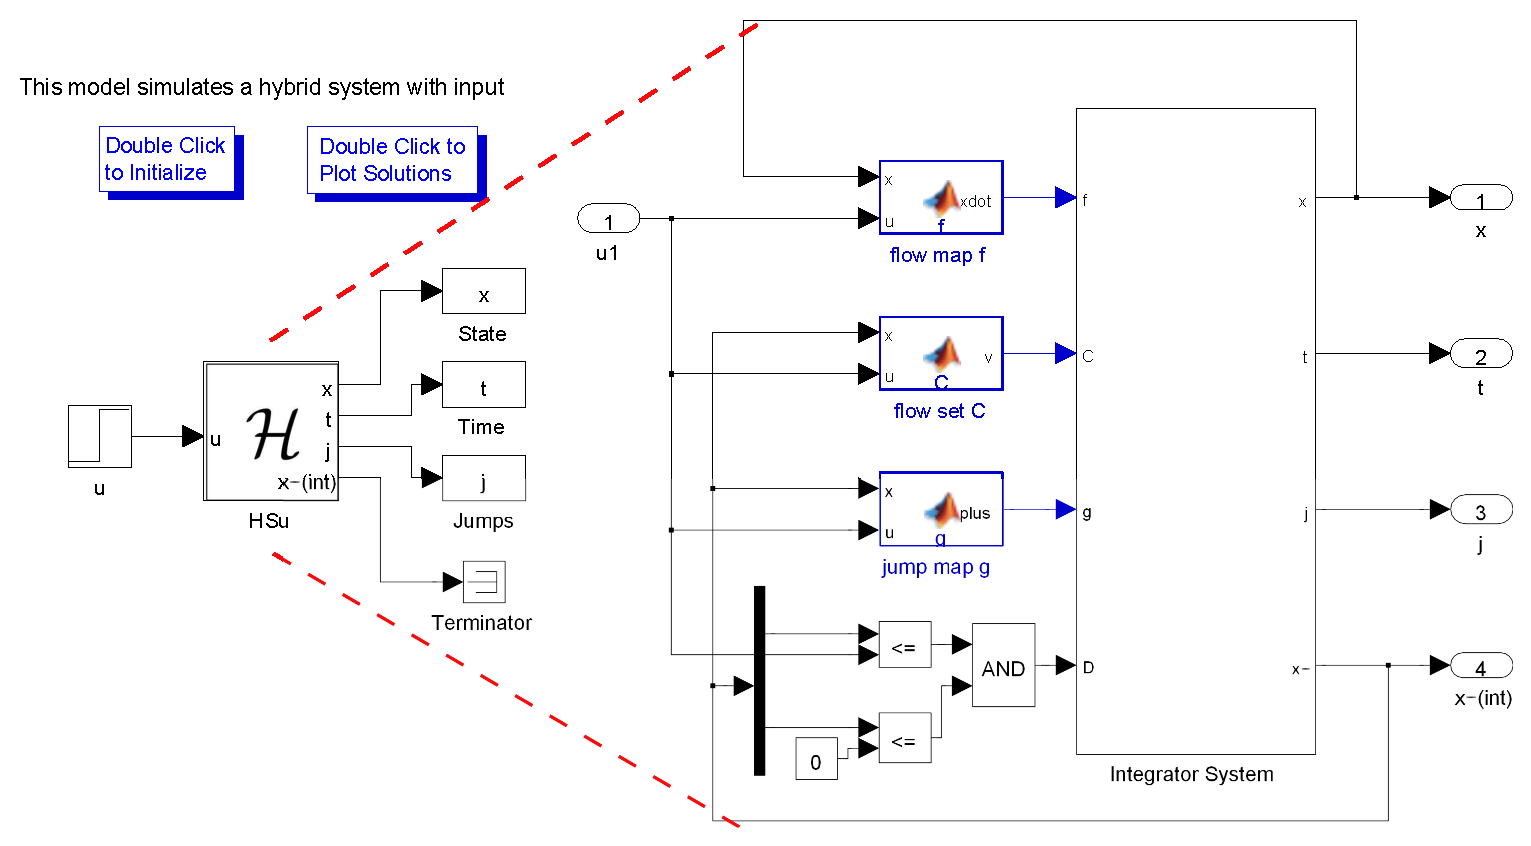
\includegraphics[width=.95\textwidth]{figures/Simulink/HybridSimulatorBBblocks}}
   \caption{Simulink implementation of bouncing ball example with operator blocks}
\label{fig:bbblocks}
  \end{center}
\end{figure}

For MATLAB/Simulink files corresponding to this alternative implementation, see Examples/Example\_\ref{ex:bbblocks}.

\end{example}


% \begin{example}{vehicle following a track with boundaries}
\label{ex:dubinspath}
Consider a vehicle modeled by a Dubins vehicle model traveling along a given track with state vector $x=[\xi_1, \xi_2, \xi_3]^\top$ with dynamics given by $\dot{\xi_1}=u\cos{\xi_3}$, $\dot{\xi_2}=u\sin{\xi_3}$, and $\dot{\xi_3}=-\xi_3+r(q)$. The input $u$ is the tangential velocity of the vehicle, $\xi_1$ and $\xi_2$ describe the vehicle's position on the plane, and $\xi_3$ is the vehicle's orientation angle. Also consider a switching controller attempting to keep the vehicle inside the boundaries of a track given by $\{(\xi_1,\xi_2):-1\leq\xi_1\leq1\}$. A state $q \in \{1,2\}$ is used to define the modes of operation of the controller. When $q=1$, the vehicle is traveling to the left, and when $q=2$, the vehicle is traveling to the right. A logic variable $r$ is defined in order to steer the vehicle back inside the boundary. The state of the closed-loop system is given by $x := [\xi^\top\ q]^\top$. A model of such a closed-loop system is given by
\begin{eqnarray}
f(x,u) & := & \left[
\begin{array}{c}
 \left[
\begin{array}{c}
   u\cos(\xi_3) \\
   u\sin(\xi_3)\\
   -\xi_3+r(q)\\
\end{array} \right] \\
u
\end{array} \right], \hspace{.1in}
r(q) := \left\{
\begin{array}{c}
\frac{3\pi}{4} \hspace{.1in} $if$ \hspace{.1in} q=1\\
\frac{\pi}{4} \hspace{.1in} $if$ \hspace{.1in} q=2 \\
\end{array} \right. \\
C & : = & \defset{(\xi,u)\in \Re^{3}\times\{1,2\}\times \Re}{(\xi_1 \leq 1 , q = 2) \mbox { or } (\xi_1 \geq -1 , q=1)}, \\
g(\xi,u) &:=&
\left\{
\begin{array}{ll}
\matt{\xi \\ 2 }
& $if$ \hspace{.15in} \xi_1\leq-1, \hspace{.1in} q=1\\
\matt{\xi \\ 1 }
& $if$ \hspace{.15in} \xi_1\geq 1, \hspace{.1in} q=2
\end{array} \right. ,\\
    D\ &: =&\defset{(\xi,u)\in \Re^{3}\times\{1,2\} \times \Re}{(\xi_1 \geq 1 ,  q = 2) \mbox { or } (\xi_1 \leq -1 ,  q=1)}
%(\Re^{2}\times\Re) \setminus C
\end{eqnarray}

The MATLAB scripts in each of the function blocks of the implementation above are given as follows. The tangential velocity of the vehicle is chosen to be $u=1$, the initial position on the plane is chosen to be $(\xi_1,\xi_2)=(0,0)$, and the initial orientation angle is chosen to be $\xi_3=\frac{\pi}{4}$ radians.

%\begin{figure}[ht]
%  \begin{center}
%  \psfrag{flows [t]}[c]{flows [$t$]}
%  \psfrag{jumps [j]}[c]{jumps [$j$]}
%  \psfrag{xi1}[c]{$\xi_1$}
%    {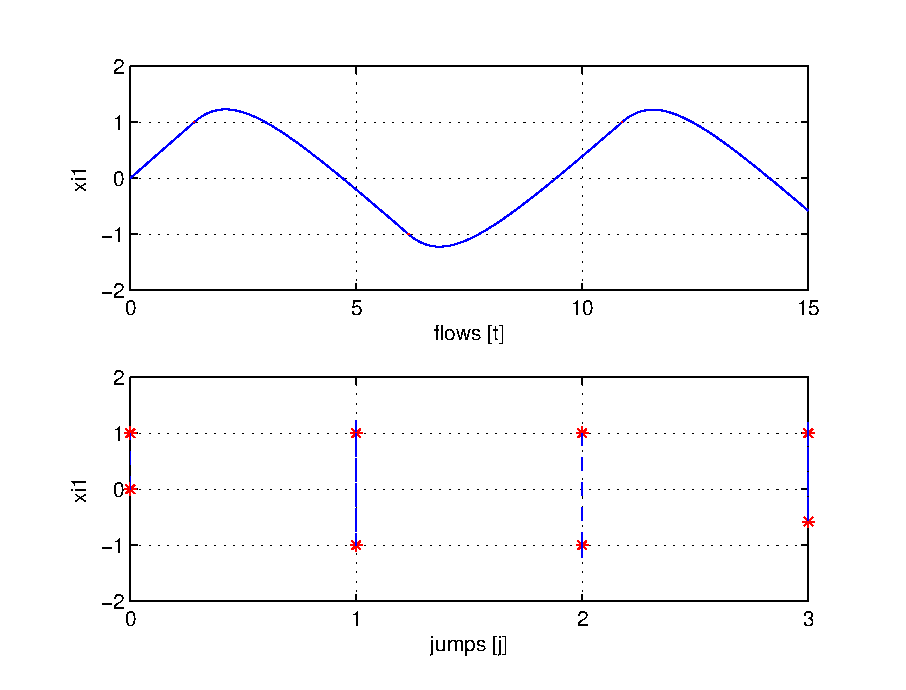
\includegraphics[width=.8\textwidth]{figures/Examples/DubinsFlowsJumps.eps}}
%   \caption{Solution of Example~\ref{ex:dubinspath}: trajectory}
%\label{fig:Dubins-1}
%  \end{center}
%\end{figure}
%
%\begin{figure}[ht]
%  \begin{center}
%  \psfrag{t}[c]{$t$}
%  \psfrag{j}[c]{$j$}
%  \psfrag{xi1}[c]{$\xi_1$}
%    {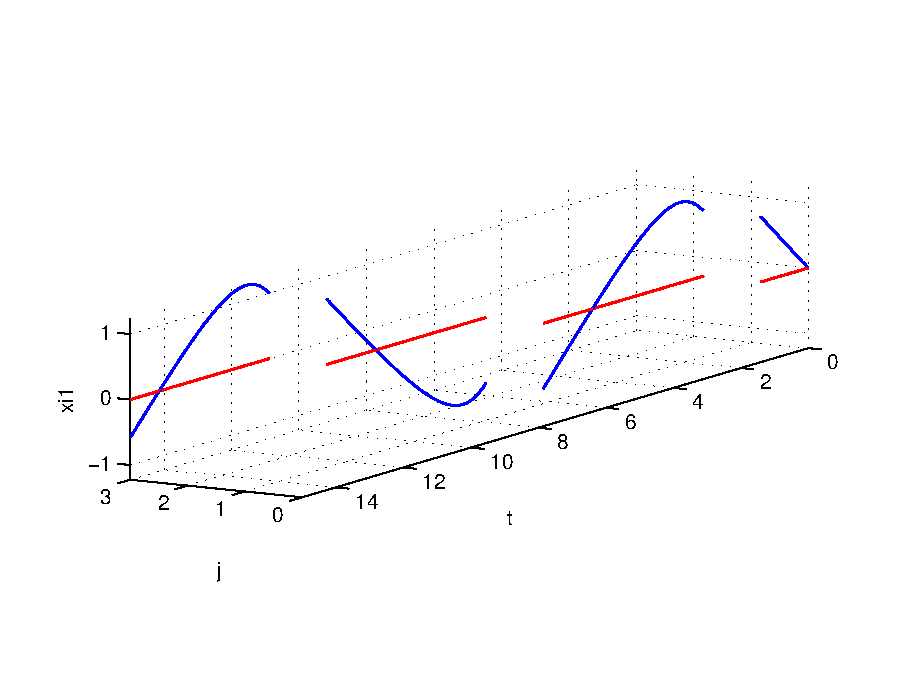
\includegraphics[width=.8\textwidth]{figures/Examples/DubinsHybridArc.eps}}
%   \caption{Hybrid arc corresponding to a solution of Example~\ref{ex:dubinspath}: trajectory}
%\label{fig:Dubins-2}
%  \end{center}
%\end{figure}

\begin{figure}[ht]
  \centering
  \psfrag{flows [t]}[c]{flows [$t$]}
  \psfrag{jumps [j]}[c]{jumps [$j$]}
  \psfrag{t}[c]{$t$}
  \psfrag{j}[c]{$j$}
  \psfrag{xi1}[c]{$\xi_1$}
  \psfrag{xi1}[c]{$\xi_1$}
\subfigure[Trajectory]{
    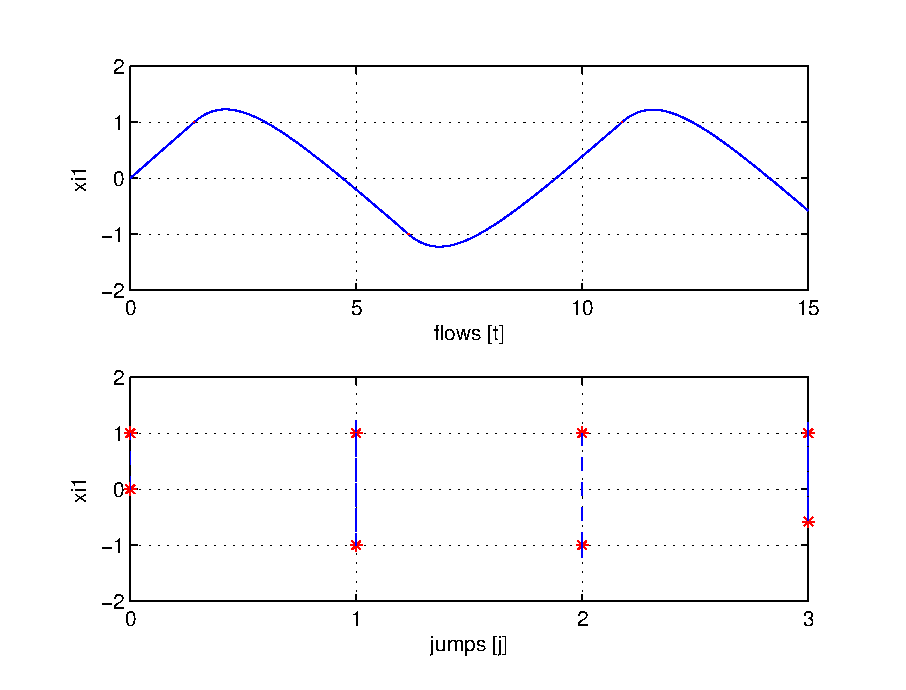
\includegraphics[width=.45\textwidth]{figures/Examples/DubinsFlowsJumps.eps}
\label{fig:Dubins-1}}
\qquad
\subfigure[Hybrid arc]{
    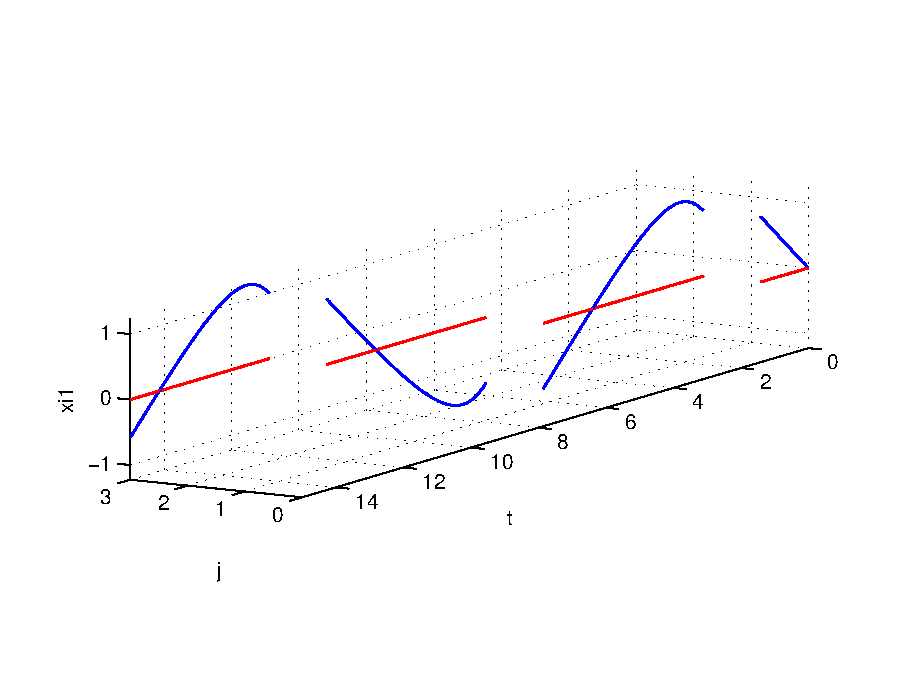
\includegraphics[width=.45\textwidth]{figures/Examples/DubinsHybridArc.eps}
\label{fig:Dubins-2}}
   \caption{Solution of Example~\ref{ex:dubinspath}}
\end{figure}

%\scriptsize
% This file was automatically created from the m-file 
% "m2tex.m" written by USL. 
% The fontencoding in this file is UTF-8. 
%  
% You will need to include the following two packages in 
% your LaTeX-Main-File. 
%  
% \usepackage{color} 
% \usepackage{fancyvrb} 
%  
% It is advised to use the following option for Inputenc 
% \usepackage[utf8]{inputenc} 
%  
  
% definition of matlab colors: 
\definecolor{mblue}{rgb}{0,0,1} 
\definecolor{mgreen}{rgb}{0.13333,0.5451,0.13333} 
\definecolor{mred}{rgb}{0.62745,0.12549,0.94118} 
\definecolor{mgrey}{rgb}{0.5,0.5,0.5} 
\definecolor{mdarkgrey}{rgb}{0.25,0.25,0.25} 
  
\DefineShortVerb[fontfamily=courier,fontseries=m]{\$} 
\DefineShortVerb[fontfamily=courier,fontseries=b]{\#} 
  
\noindent                    
 \hspace*{-1.6em}{\scriptsize 1}$  $\color{mblue}$function$\color{black}$ xdot = f(x, u, gamma)$\\
 \hspace*{-1.6em}{\scriptsize 2}$  $\\
 \hspace*{-1.6em}{\scriptsize 3}$  $\color{mgreen}#%%%%%%%%%%%%%%%%%%%%%%%%%%%%%%%%%%%%%%%%%%%%%%%%%%%%%%%%%%%%%%%%%%%%%%%%%%%#\color{black}$$\\
 \hspace*{-1.6em}{\scriptsize 4}$  $\color{mgreen}$% Matlab Function  Author: Ricardo Sanfelice $\color{black}$$\\
 \hspace*{-1.6em}{\scriptsize 5}$  $\color{mgreen}$% (Revised by Giampiero Campa)$\color{black}$$\\
 \hspace*{-1.6em}{\scriptsize 6}$  $\color{mgreen}$% (Revised by Pablo Nanez)$\color{black}$$\\
 \hspace*{-1.6em}{\scriptsize 7}$  $\color{mgreen}$%$\color{black}$$\\
 \hspace*{-1.6em}{\scriptsize 8}$  $\color{mgreen}$% Project: Simulation of a hybrid system (Bouncing Ball)$\color{black}$$\\
 \hspace*{-1.6em}{\scriptsize 9}$  $\color{mgreen}$%$\color{black}$$\\
 \hspace*{-2em}{\scriptsize 10}$  $\color{mgreen}$% Name: f.m$\color{black}$$\\
 \hspace*{-2em}{\scriptsize 11}$  $\color{mgreen}$%$\color{black}$$\\
 \hspace*{-2em}{\scriptsize 12}$  $\color{mgreen}$% Description: Flow map$\color{black}$$\\
 \hspace*{-2em}{\scriptsize 13}$  $\color{mgreen}$%$\color{black}$$\\
 \hspace*{-2em}{\scriptsize 14}$  $\color{mgreen}$% Version: 1.0$\color{black}$$\\
 \hspace*{-2em}{\scriptsize 15}$  $\color{mgreen}$% Required files: - $\color{black}$$\\
 \hspace*{-2em}{\scriptsize 16}$  $\color{mgreen}#%%%%%%%%%%%%%%%%%%%%%%%%%%%%%%%%%%%%%%%%%%%%%%%%%%%%%%%%%%%%%%%%%%%%%%%%%%%#\color{black}$$\\
 \hspace*{-2em}{\scriptsize 17}$  $\\
 \hspace*{-2em}{\scriptsize 18}$  $\\
 \hspace*{-2em}{\scriptsize 19}$  $\color{mgreen}$% flow map: xdot=f(x,u);$\color{black}$$\\
 \hspace*{-2em}{\scriptsize 20}$  xdot = [x(2); gamma];$\\ 
  
\UndefineShortVerb{\$} 
\UndefineShortVerb{\#}\label{scr:f}
%\normalsize

%\scriptsize
% This file was automatically created from the m-file 
% "m2tex.m" written by USL. 
% The fontencoding in this file is UTF-8. 
%  
% You will need to include the following two packages in 
% your LaTeX-Main-File. 
%  
% \usepackage{color} 
% \usepackage{fancyvrb} 
%  
% It is advised to use the following option for Inputenc 
% \usepackage[utf8]{inputenc} 
%  
  
% definition of matlab colors: 
\definecolor{mblue}{rgb}{0,0,1} 
\definecolor{mgreen}{rgb}{0.13333,0.5451,0.13333} 
\definecolor{mred}{rgb}{0.62745,0.12549,0.94118} 
\definecolor{mgrey}{rgb}{0.5,0.5,0.5} 
\definecolor{mdarkgrey}{rgb}{0.25,0.25,0.25} 
  
\DefineShortVerb[fontfamily=courier,fontseries=m]{\$} 
\DefineShortVerb[fontfamily=courier,fontseries=b]{\#} 
  
\noindent                          
 \hspace*{-1.6em}{\scriptsize 1}$  $\color{mblue}$function$\color{black}$ v  = C(x, u)$\\
 \hspace*{-1.6em}{\scriptsize 2}$  $\color{mgreen}$%--------------------------------------------------------------------------$\color{black}$$\\
 \hspace*{-1.6em}{\scriptsize 3}$  $\color{mgreen}$% Matlab M-file Project: HyEQ Toolbox @  Hybrid Systems Laboratory (HSL),$\color{black}$$\\
 \hspace*{-1.6em}{\scriptsize 4}$  $\color{mgreen}$% https://hybrid.soe.ucsc.edu/software$\color{black}$$\\
 \hspace*{-1.6em}{\scriptsize 5}$  $\color{mgreen}$% http://hybridsimulator.wordpress.com/$\color{black}$$\\
 \hspace*{-1.6em}{\scriptsize 6}$  $\color{mgreen}$%--------------------------------------------------------------------------$\color{black}$$\\
 \hspace*{-1.6em}{\scriptsize 7}$  $\color{mgreen}$% Project: Simulation of a hybrid system$\color{black}$$\\
 \hspace*{-1.6em}{\scriptsize 8}$  $\color{mgreen}$% Description: Flow set$\color{black}$$\\
 \hspace*{-1.6em}{\scriptsize 9}$  $\color{mgreen}$%--------------------------------------------------------------------------$\color{black}$$\\
 \hspace*{-2em}{\scriptsize 10}$  $\color{mgreen}$%--------------------------------------------------------------------------$\color{black}$$\\
 \hspace*{-2em}{\scriptsize 11}$  $\color{mgreen}$%   See also HYEQSOLVER, PLOTARC, PLOTARC3, PLOTFLOWS, PLOTHARC,$\color{black}$$\\
 \hspace*{-2em}{\scriptsize 12}$  $\color{mgreen}$%   PLOTHARCCOLOR, PLOTHARCCOLOR3D, PLOTHYBRIDARC, PLOTJUMPS.$\color{black}$$\\
 \hspace*{-2em}{\scriptsize 13}$  $\color{mgreen}$%   Copyright @ Hybrid Systems Laboratory (HSL),$\color{black}$$\\
 \hspace*{-2em}{\scriptsize 14}$  $\color{mgreen}$%   Revision: 0.0.0.3 Date: 05/20/2015 3:42:00$\color{black}$$\\
 \hspace*{-2em}{\scriptsize 15}$  $\color{mgreen}$%$\color{black}$$\\
 \hspace*{-2em}{\scriptsize 16}$  $\color{mgreen}$% Check on flow conditions$\color{black}$$\\
 \hspace*{-2em}{\scriptsize 17}$  $\color{mgreen}$% E.g.,$\color{black}$$\\
 \hspace*{-2em}{\scriptsize 18}$  $\color{mgreen}$% if (x(1) >= u(1))  % flow condition$\color{black}$$\\
 \hspace*{-2em}{\scriptsize 19}$  $\color{mgreen}$%     v = 1;  % report flow$\color{black}$$\\
 \hspace*{-2em}{\scriptsize 20}$  $\color{mgreen}$% else$\color{black}$$\\
 \hspace*{-2em}{\scriptsize 21}$  $\color{mgreen}$%     v = 0;   % do not report flow$\color{black}$$\\
 \hspace*{-2em}{\scriptsize 22}$  $\color{mgreen}$% end$\color{black}$$\\
 \hspace*{-2em}{\scriptsize 23}$  $\\
 \hspace*{-2em}{\scriptsize 24}$  $\\
 \hspace*{-2em}{\scriptsize 25}$  v = 1; $\color{mgreen}$% report flow$\color{black}$$\\
 \hspace*{-2em}{\scriptsize 26}$  $\\ 
  
\UndefineShortVerb{\$} 
\UndefineShortVerb{\#}\label{scr:C}
%\normalsize

%\scriptsize
% This file was automatically created from the m-file 
% "m2tex.m" written by USL. 
% The fontencoding in this file is UTF-8. 
%  
% You will need to include the following two packages in 
% your LaTeX-Main-File. 
%  
% \usepackage{color} 
% \usepackage{fancyvrb} 
%  
% It is advised to use the following option for Inputenc 
% \usepackage[utf8]{inputenc} 
%  
  
% definition of matlab colors: 
\definecolor{mblue}{rgb}{0,0,1} 
\definecolor{mgreen}{rgb}{0.13333,0.5451,0.13333} 
\definecolor{mred}{rgb}{0.62745,0.12549,0.94118} 
\definecolor{mgrey}{rgb}{0.5,0.5,0.5} 
\definecolor{mdarkgrey}{rgb}{0.25,0.25,0.25} 
  
\DefineShortVerb[fontfamily=courier,fontseries=m]{\$} 
\DefineShortVerb[fontfamily=courier,fontseries=b]{\#} 
  
\noindent   
 \hspace*{-1.6em}{\scriptsize 1}$  $\color{mblue}$function$\color{black}$ xplus = g(x, u, lambda)$\\
 \hspace*{-1.6em}{\scriptsize 2}$  $\color{mgreen}$% jump map$\color{black}$$\\
 \hspace*{-1.6em}{\scriptsize 3}$  xplus = [u(1); -lambda*x(2)];$\\ 
  
\UndefineShortVerb{\$} 
\UndefineShortVerb{\#}\label{scr:g}
%\normalsize

%\scriptsize
% This file was automatically created from the m-file 
% "m2tex.m" written by USL. 
% The fontencoding in this file is UTF-8. 
%  
% You will need to include the following two packages in 
% your LaTeX-Main-File. 
%  
% \usepackage{color} 
% \usepackage{fancyvrb} 
%  
% It is advised to use the following option for Inputenc 
% \usepackage[utf8]{inputenc} 
%  
  
% definition of matlab colors: 
\definecolor{mblue}{rgb}{0,0,1} 
\definecolor{mgreen}{rgb}{0.13333,0.5451,0.13333} 
\definecolor{mred}{rgb}{0.62745,0.12549,0.94118} 
\definecolor{mgrey}{rgb}{0.5,0.5,0.5} 
\definecolor{mdarkgrey}{rgb}{0.25,0.25,0.25} 
  
\DefineShortVerb[fontfamily=courier,fontseries=m]{\$} 
\DefineShortVerb[fontfamily=courier,fontseries=b]{\#} 
  
\noindent                         
 \hspace*{-1.6em}{\scriptsize 1}$  $\color{mblue}$function$\color{black}$ v  = D(x, u) $\\
 \hspace*{-1.6em}{\scriptsize 2}$  $\\
 \hspace*{-1.6em}{\scriptsize 3}$  $\color{mgreen}#%%%%%%%%%%%%%%%%%%%%%%%%%%%%%%%%%%%%%%%%%%%%%%%%%%%%%%%%%%%%%%%%%%%%%%%%%%%#\color{black}$$\\
 \hspace*{-1.6em}{\scriptsize 4}$  $\color{mgreen}$% Matlab Function  Author: Ricardo Sanfelice $\color{black}$$\\
 \hspace*{-1.6em}{\scriptsize 5}$  $\color{mgreen}$% (Revised by Giampiero Campa)$\color{black}$$\\
 \hspace*{-1.6em}{\scriptsize 6}$  $\color{mgreen}$% (Revised by Pablo Nanez)$\color{black}$$\\
 \hspace*{-1.6em}{\scriptsize 7}$  $\color{mgreen}$%$\color{black}$$\\
 \hspace*{-1.6em}{\scriptsize 8}$  $\color{mgreen}$% Project: Simulation of a hybrid system (Bouncing ball)$\color{black}$$\\
 \hspace*{-1.6em}{\scriptsize 9}$  $\color{mgreen}$%$\color{black}$$\\
 \hspace*{-2em}{\scriptsize 10}$  $\color{mgreen}$% Name: D.m$\color{black}$$\\
 \hspace*{-2em}{\scriptsize 11}$  $\color{mgreen}$%$\color{black}$$\\
 \hspace*{-2em}{\scriptsize 12}$  $\color{mgreen}$% Description: Jump set$\color{black}$$\\
 \hspace*{-2em}{\scriptsize 13}$  $\color{mgreen}$%$\color{black}$$\\
 \hspace*{-2em}{\scriptsize 14}$  $\color{mgreen}$% Version: 1.0$\color{black}$$\\
 \hspace*{-2em}{\scriptsize 15}$  $\color{mgreen}$% Required files: - $\color{black}$$\\
 \hspace*{-2em}{\scriptsize 16}$  $\color{mgreen}#%%%%%%%%%%%%%%%%%%%%%%%%%%%%%%%%%%%%%%%%%%%%%%%%%%%%%%%%%%%%%%%%%%%%%%%%%%%#\color{black}$$\\
 \hspace*{-2em}{\scriptsize 17}$  $\\
 \hspace*{-2em}{\scriptsize 18}$  xtemp = zeros(2,1);$\\
 \hspace*{-2em}{\scriptsize 19}$  xtemp = x;$\\
 \hspace*{-2em}{\scriptsize 20}$  $\\
 \hspace*{-2em}{\scriptsize 21}$  $\color{mblue}$if$\color{black}$ (xtemp(1) <= u(1)) && (xtemp(2) <= 0)  $\color{mgreen}$% jump condition$\color{black}$$\\
 \hspace*{-2em}{\scriptsize 22}$      v = 1;  $\color{mgreen}$% report jump$\color{black}$$\\
 \hspace*{-2em}{\scriptsize 23}$  $\color{mblue}$else$\color{black}$$\\
 \hspace*{-2em}{\scriptsize 24}$      v = 0;   $\color{mgreen}$% do not report jump$\color{black}$$\\
 \hspace*{-2em}{\scriptsize 25}$  $\color{mblue}$end$\color{black}$$\\ 
  
\UndefineShortVerb{\$} 
\UndefineShortVerb{\#}\label{scr:D}
%\normalsize


A solution to the system of a vehicle following a track in $\{(\xi_1,\xi_2):-1\leq \xi_1 \leq1\}$, and with
$T=15, J=10$, $rule =1$, is depicted in Figure~\ref{fig:Dubins-1} (trajectory).  Both the
projection onto $t$ and $j$ are shown. Figure~\ref{fig:Dubins-2} depicts the corresponding
hybrid arc.

For MATLAB/Simulink files of this example, see Examples/Example\_\ref{ex:dubinspath}.

\end{example}



% 
\begin{example}{interconnection of hybrid systems $\HS_1$ (bouncing ball) and $\HS_2$ (moving platform)}
\label{ex:interconnection1}
Consider a bouncing ball ($\HS_1$) bouncing on a platform ($\HS_2$) at some initial height and converging to the ground at zero height. This is an interconnection problem because the current states of each system affect the behavior of the other system. In this interconnection, the bouncing ball will contact the platform, bounce back up, and cause a jump in height of the platform so that it gets closer to the ground. After some time, both the ball and the platform will converge to the ground. In order to model this system, the output of the bouncing ball becomes the input of the moving platform, and vice versa. For the simulation of the described system with regular data where $\HS_1$ is given by

\begin{eqnarray}
f_1(\xi, u_1,v_1):=\left[
 \begin{array}{c}
   \xi_2 \\
 -\gamma - b\xi_2 +v_{11}
 \end{array}
\right],
   C_1 : = \defset{(\xi,u_1)}{\xi_1 \geq u_1, u_1 \geq 0}\\
g_1(\xi, u_1, v_1):=\left[ \begin{array}{c}
 \xi_1+\alpha_1\xi_2^2 \\
e_1|\xi_2| + v_{12}
\end{array}
\right]\ ,
    D_1: =\defset{(\xi,u_1)}{\xi_1 =u_1, u_1 \geq 0},
y_1 = h_1(\xi) : =\xi_1
\end{eqnarray}
where $\gamma, b, \alpha_1 >0, e_1 \in [0,1)$, $\xi = [\xi_1 , \xi_2]^\top$ is the state, $y_1 \in \Re$ is the output, $u_1 \in \Re$ and $v_1 = [v_{11} , v_{12}]^\top \in \Re^{2}$ are the inputs, and the hybrid system $\HS_2$ is given by

\begin{eqnarray}
f_2(\eta,u_2,v_2):=\left[
 \begin{array}{c}
   \eta_2 \\
 -\eta_1-2\eta_2 +v_{12}
 \end{array}
\right],
   C_2 : = \defset{(\eta,u_2)}{\eta_1 \leq u_2, \eta_1 \geq 0}\\
g_2(\eta,u_2,v_2):=\left[ \begin{array}{c}
 \eta_1-\alpha_2|\eta_2| \\
-e_2|\eta_2| + v_{22}
\end{array}
\right]\ ,
    D_2: =\defset{(\eta,u_2)}{\eta_1 = u_2, \eta_1 \geq 0},
y_2 = h_2(\eta) : = \eta_1
\end{eqnarray}
where $\alpha_2 >0, e_2 \in [0,1)$, $\eta = [\eta_1 , \eta_2]^\top \in \Re^{2}$ is the state,
$y_2 \in \Re$ is the output, and $u_2 \in \Re$ and $v_2 = [v_{21} , v_{22}]^\top \in \Re^{2}$
are the inputs.

Therefore, the interconnection may be defined by the input assignment
\begin{equation}
u_1 = y_2,   \hspace{5mm}     u_2 = y_1.
\end{equation}

The signals $v_1$  and $v_2$ are included as external inputs in the model in order to simulate the effects of environmental perturbations, such as a wind gust, on the system.

The MATLAB scripts in each of the function blocks of the implementation above are given as follows. The constants for
the interconnected system are $\gamma = 0.8$, $b=0.1$, and $\alpha_1, \alpha_2=0.1$.

\begin{figure}[ht!]
  \begin{center}
    {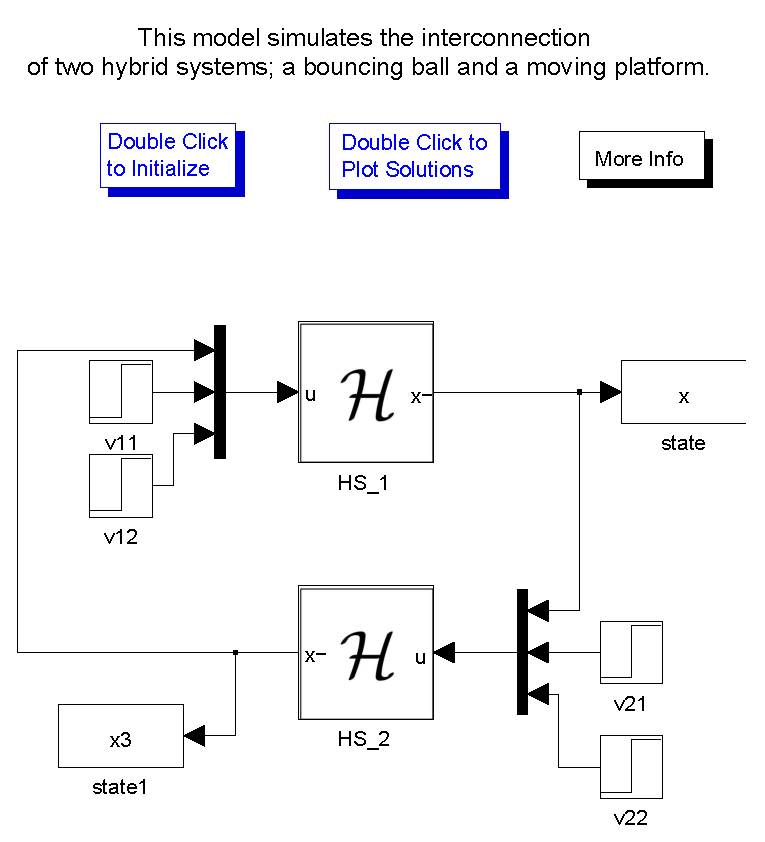
\includegraphics[width=.6\textwidth]{figures/Simulink/InterconnectionMdl.eps}}
   \caption{MATLAB/Simulink implementation of interconnected hybrid systems $\HS_1$ and
$\HS_2$}
\label{fig:interconnection-1}
  \end{center}
\end{figure}

\begin{figure}[ht!]
  \begin{center}
  \psfrag{flows [t]}[c]{flows [$t$]}
  \psfrag{jumps [j]}[c]{jumps [$j$]}
  \psfrag{xi1, eta1}[c]{$\xi_1, \eta_1$}
  \psfrag{xi2, eta2}[c]{$\xi_2, \eta_2$}
    {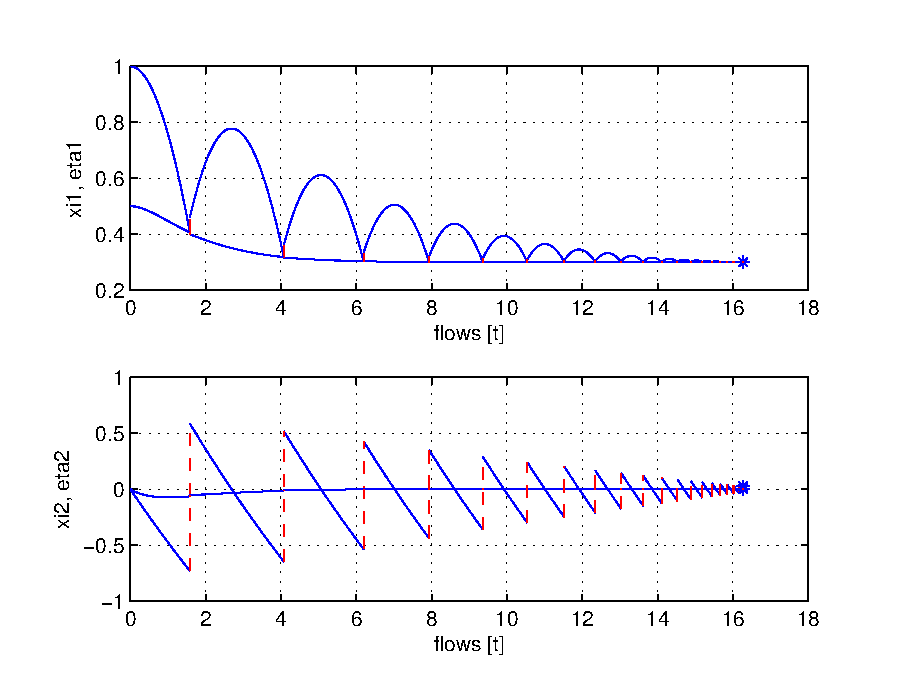
\includegraphics[width=.8\textwidth]{figures/Examples/InterconnectionH1H2.eps}}
   \caption{Solution of Example~\ref{ex:interconnection1}: height and velocity}
\label{fig:interconnection-2}
  \end{center}
\end{figure}

%\begin{figure}[ht]
%  \begin{center}
%  \psfrag{flows [t]}[c]{flows [$t$]}
%  \psfrag{jumps [j]}[c]{jumps [$j$]}
%  \psfrag{xi1}[c]{$\xi_1$}
%    {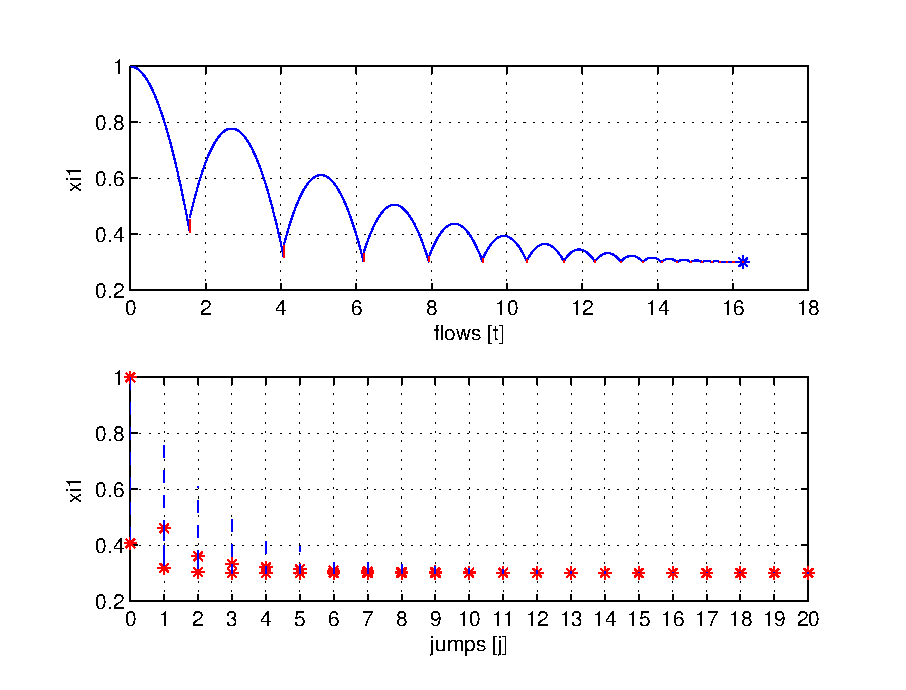
\includegraphics[width=.8\textwidth]{figures/Examples/InterconnectionH1.eps}}
%   \caption{Solution of Example~\ref{ex:interconnection1} for system $\HS_1$: height}
%\label{fig:interconnection-3}
%  \end{center}
%\end{figure}
%
%\begin{figure}[ht]
%  \begin{center}
%  \psfrag{flows [t]}[c]{flows [$t$]}
%  \psfrag{jumps [j]}[c]{jumps [$j$]}
%  \psfrag{xi2}[c]{$\xi_2$}
%    {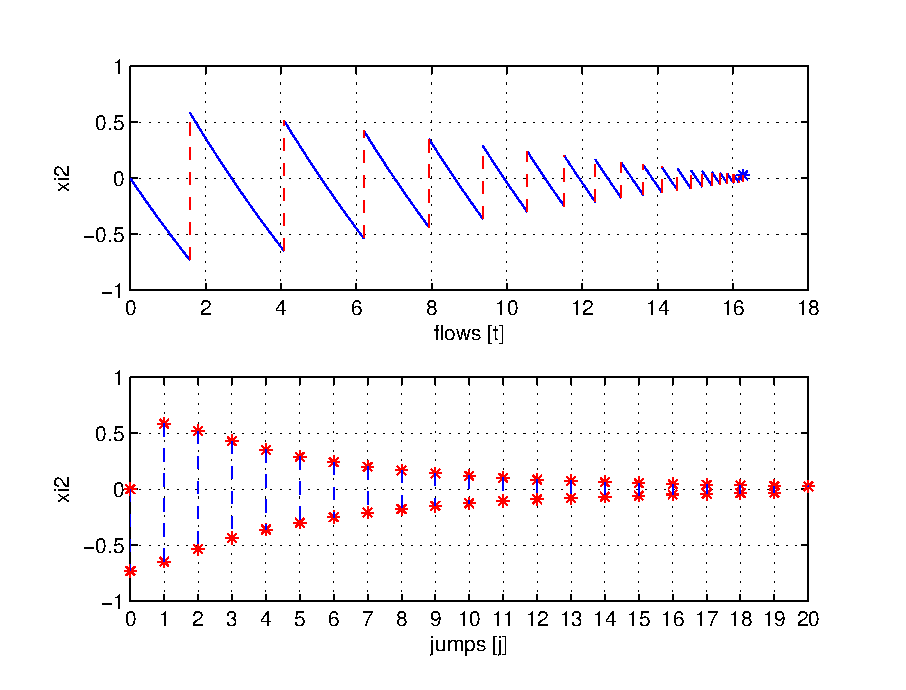
\includegraphics[width=.8\textwidth]{figures/Examples/InterconnectionH1velocity.eps}}
%   \caption{Solution of Example~\ref{ex:interconnection1} for system $\HS_1$: velocity}
%\label{fig:interconnection-4}
%  \end{center}
%\end{figure}

\begin{figure}[ht]
  \centering
  \psfrag{flows [t]}[c]{flows [$t$]}
  \psfrag{jumps [j]}[c]{jumps [$j$]}
  \psfrag{xi1}[c]{$\xi_1$}
  \psfrag{xi2}[c]{$\xi_2$}
\subfigure[Height]{
    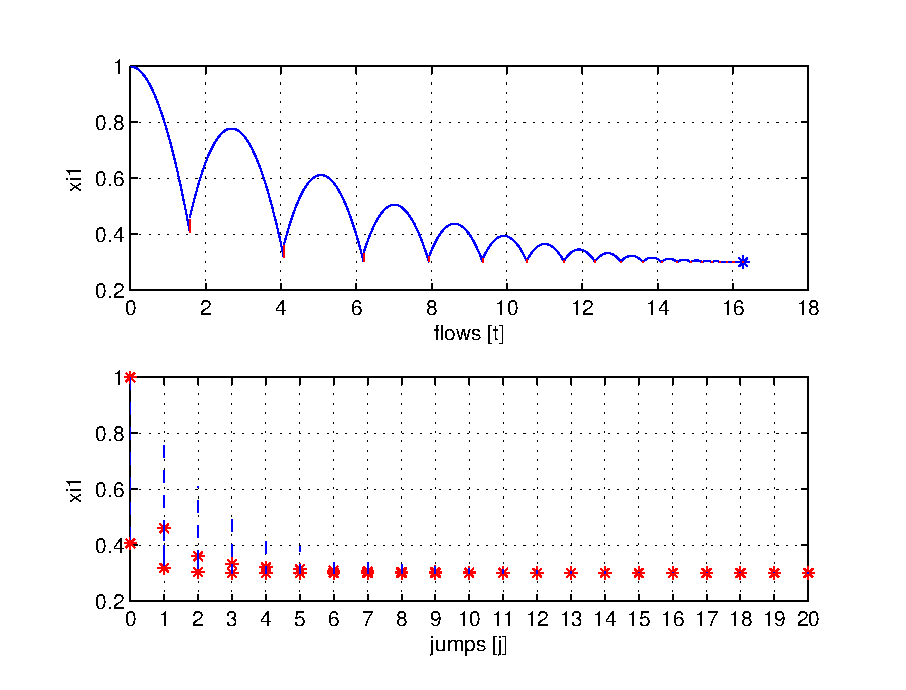
\includegraphics[width=.45\textwidth]{figures/Examples/InterconnectionH1.eps}
\label{fig:interconnection-3}}
\qquad
\subfigure[Velocity]{
    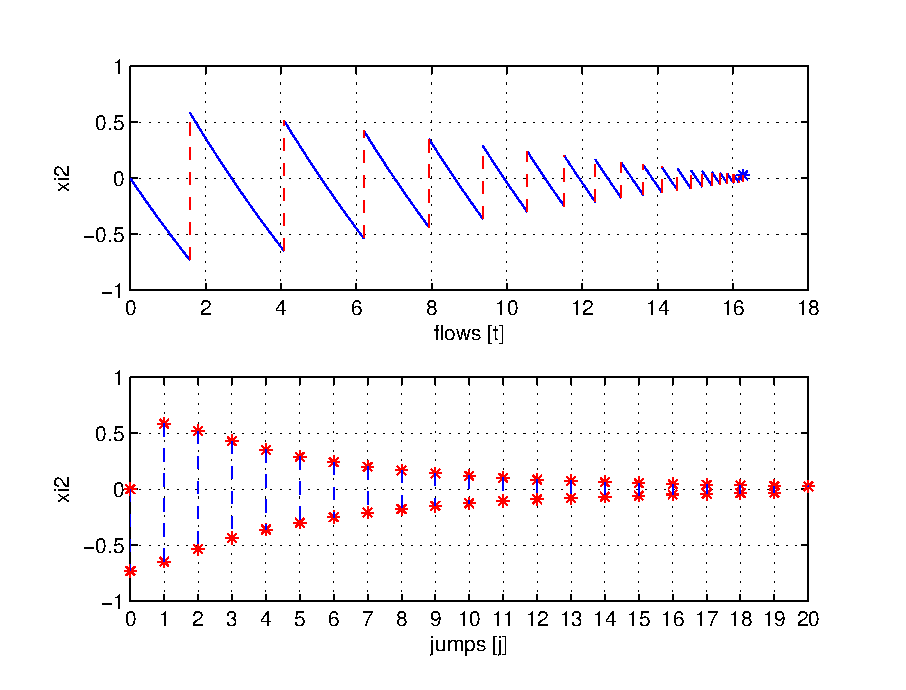
\includegraphics[width=.45\textwidth]{figures/Examples/InterconnectionH1velocity.eps}
\label{fig:interconnection-4}}
\caption{Solution of Example \ref{ex:interconnection1} for system $\HS_1$}
\end{figure}

%\begin{figure}[ht]
%  \begin{center}
%  \psfrag{flows [t]}[c]{flows [$t$]}
%  \psfrag{jumps [j]}[c]{jumps [$j$]}
%  \psfrag{eta1}[c]{$\eta_1$}
%    {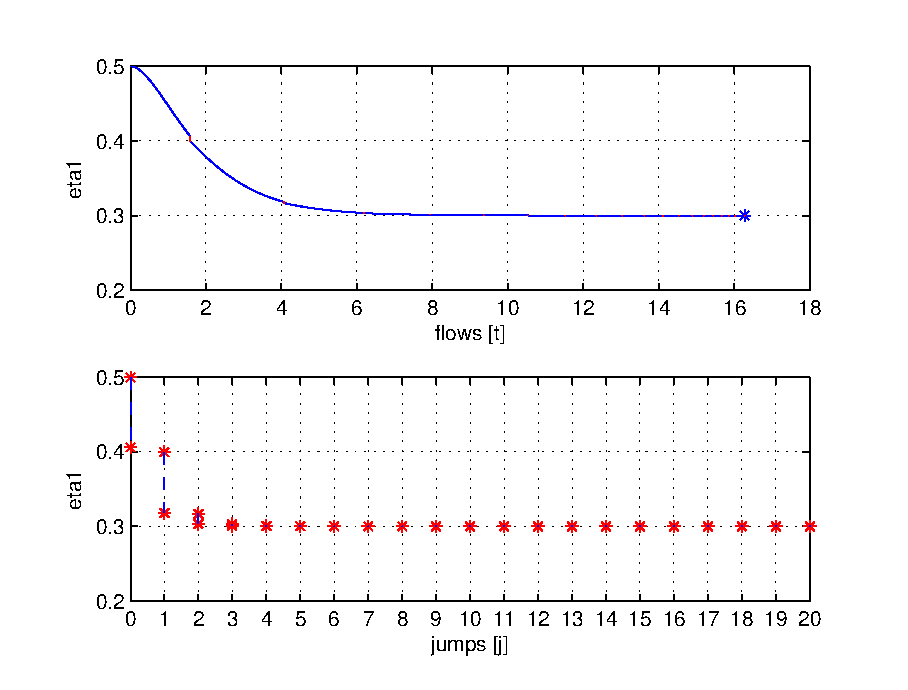
\includegraphics[width=.8\textwidth]{figures/Examples/InterconnectionH2.eps}}
%   \caption{Solution of Example~\ref{ex:interconnection1} for system $\HS_2$: height}
%\label{fig:interconnection-5}
%  \end{center}
%\end{figure}
%
%\begin{figure}[ht]
%  \begin{center}
%  \psfrag{flows [t]}[c]{flows [$t$]}
%  \psfrag{jumps [j]}[c]{jumps [$j$]}
%  \psfrag{eta2}[c]{$\eta_2$}
%    {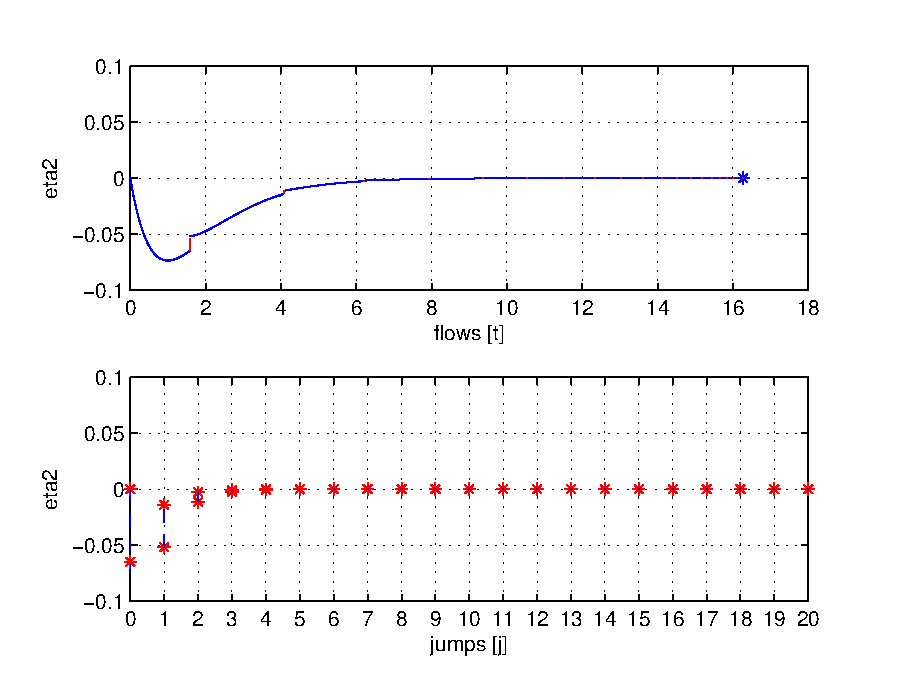
\includegraphics[width=.8\textwidth]{figures/Examples/InterconnectionH2velocity.eps}}
%   \caption{Solution of Example~\ref{ex:interconnection1} for system $\HS_2$: velocity}
%\label{fig:interconnection-6}
%  \end{center}
%\end{figure}

\begin{figure}[ht]
  \centering
  \psfrag{flows [t]}[c]{flows [$t$]}
  \psfrag{jumps [j]}[c]{jumps [$j$]}
  \psfrag{eta1}[c]{$\eta_1$}
  \psfrag{eta2}[c]{$\eta_2$}
\subfigure[Height]{
    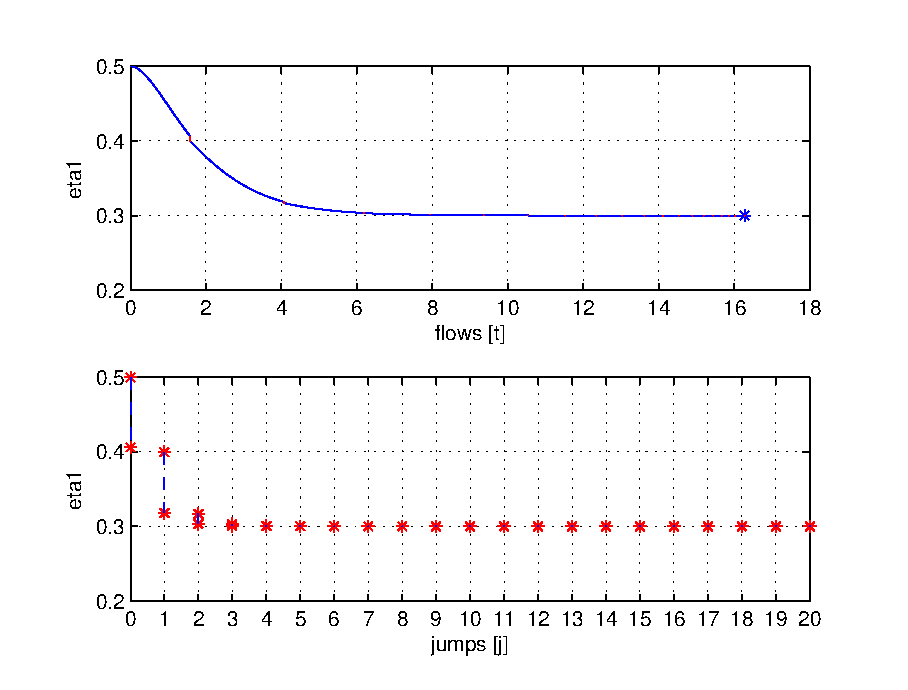
\includegraphics[width=.45\textwidth]{figures/Examples/InterconnectionH2.eps}
\label{fig:interconnection-5}}
\qquad
\subfigure[Velocity]{
    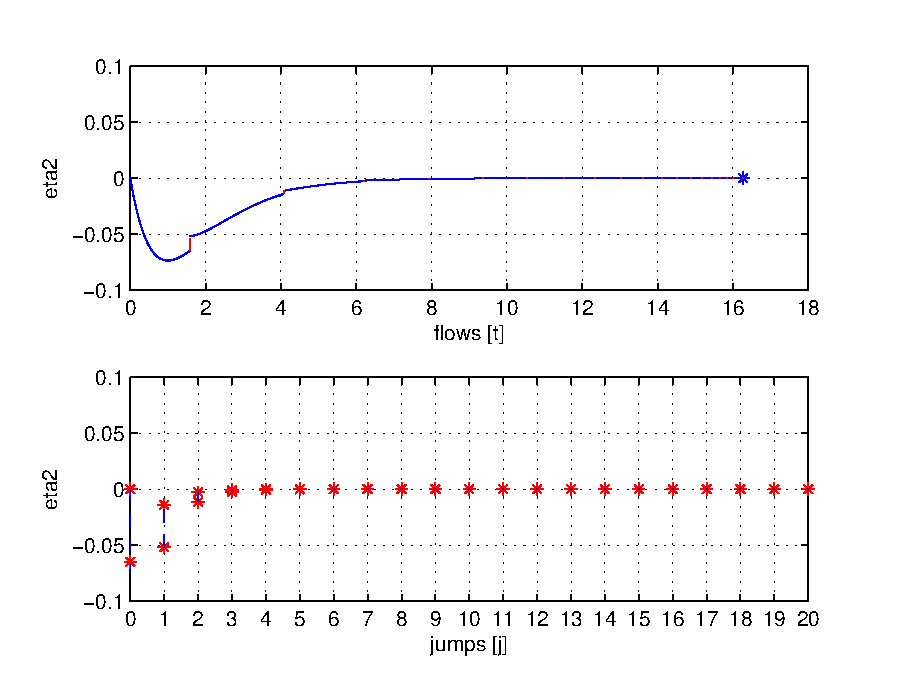
\includegraphics[width=.45\textwidth]{figures/Examples/InterconnectionH2velocity.eps}
\label{fig:interconnection-6}}
\caption{Solution of Example~\ref{ex:interconnection1} for system $\HS_2$}
\end{figure}

% Set the location for MATLAB files included via the "\code" command.
\codeLocation{Matlab2tex_1_6}

\begin{itemize}
\item For hybrid system $\HS_1$:

\code{f.m}
\code{C.m}
\code{g.m}
\code{D.m}

% Flow map
% %\scriptsize
% % This file was automatically created from the m-file 
% "m2tex.m" written by USL. 
% The fontencoding in this file is UTF-8. 
%  
% You will need to include the following two packages in 
% your LaTeX-Main-File. 
%  
% \usepackage{color} 
% \usepackage{fancyvrb} 
%  
% It is advised to use the following option for Inputenc 
% \usepackage[utf8]{inputenc} 
%  
  
% definition of matlab colors: 
\definecolor{mblue}{rgb}{0,0,1} 
\definecolor{mgreen}{rgb}{0.13333,0.5451,0.13333} 
\definecolor{mred}{rgb}{0.62745,0.12549,0.94118} 
\definecolor{mgrey}{rgb}{0.5,0.5,0.5} 
\definecolor{mdarkgrey}{rgb}{0.25,0.25,0.25} 
  
\DefineShortVerb[fontfamily=courier,fontseries=m]{\$} 
\DefineShortVerb[fontfamily=courier,fontseries=b]{\#} 
  
\noindent                    
 \hspace*{-1.6em}{\scriptsize 1}$  $\color{mblue}$function$\color{black}$ xdot = f(x, u, gamma)$\\
 \hspace*{-1.6em}{\scriptsize 2}$  $\\
 \hspace*{-1.6em}{\scriptsize 3}$  $\color{mgreen}#%%%%%%%%%%%%%%%%%%%%%%%%%%%%%%%%%%%%%%%%%%%%%%%%%%%%%%%%%%%%%%%%%%%%%%%%%%%#\color{black}$$\\
 \hspace*{-1.6em}{\scriptsize 4}$  $\color{mgreen}$% Matlab Function  Author: Ricardo Sanfelice $\color{black}$$\\
 \hspace*{-1.6em}{\scriptsize 5}$  $\color{mgreen}$% (Revised by Giampiero Campa)$\color{black}$$\\
 \hspace*{-1.6em}{\scriptsize 6}$  $\color{mgreen}$% (Revised by Pablo Nanez)$\color{black}$$\\
 \hspace*{-1.6em}{\scriptsize 7}$  $\color{mgreen}$%$\color{black}$$\\
 \hspace*{-1.6em}{\scriptsize 8}$  $\color{mgreen}$% Project: Simulation of a hybrid system (Bouncing Ball)$\color{black}$$\\
 \hspace*{-1.6em}{\scriptsize 9}$  $\color{mgreen}$%$\color{black}$$\\
 \hspace*{-2em}{\scriptsize 10}$  $\color{mgreen}$% Name: f.m$\color{black}$$\\
 \hspace*{-2em}{\scriptsize 11}$  $\color{mgreen}$%$\color{black}$$\\
 \hspace*{-2em}{\scriptsize 12}$  $\color{mgreen}$% Description: Flow map$\color{black}$$\\
 \hspace*{-2em}{\scriptsize 13}$  $\color{mgreen}$%$\color{black}$$\\
 \hspace*{-2em}{\scriptsize 14}$  $\color{mgreen}$% Version: 1.0$\color{black}$$\\
 \hspace*{-2em}{\scriptsize 15}$  $\color{mgreen}$% Required files: - $\color{black}$$\\
 \hspace*{-2em}{\scriptsize 16}$  $\color{mgreen}#%%%%%%%%%%%%%%%%%%%%%%%%%%%%%%%%%%%%%%%%%%%%%%%%%%%%%%%%%%%%%%%%%%%%%%%%%%%#\color{black}$$\\
 \hspace*{-2em}{\scriptsize 17}$  $\\
 \hspace*{-2em}{\scriptsize 18}$  $\\
 \hspace*{-2em}{\scriptsize 19}$  $\color{mgreen}$% flow map: xdot=f(x,u);$\color{black}$$\\
 \hspace*{-2em}{\scriptsize 20}$  xdot = [x(2); gamma];$\\ 
  
\UndefineShortVerb{\$} 
\UndefineShortVerb{\#}\label{scr:f}
% %\normalsize

% Flow set
% %\scriptsize
% % This file was automatically created from the m-file 
% "m2tex.m" written by USL. 
% The fontencoding in this file is UTF-8. 
%  
% You will need to include the following two packages in 
% your LaTeX-Main-File. 
%  
% \usepackage{color} 
% \usepackage{fancyvrb} 
%  
% It is advised to use the following option for Inputenc 
% \usepackage[utf8]{inputenc} 
%  
  
% definition of matlab colors: 
\definecolor{mblue}{rgb}{0,0,1} 
\definecolor{mgreen}{rgb}{0.13333,0.5451,0.13333} 
\definecolor{mred}{rgb}{0.62745,0.12549,0.94118} 
\definecolor{mgrey}{rgb}{0.5,0.5,0.5} 
\definecolor{mdarkgrey}{rgb}{0.25,0.25,0.25} 
  
\DefineShortVerb[fontfamily=courier,fontseries=m]{\$} 
\DefineShortVerb[fontfamily=courier,fontseries=b]{\#} 
  
\noindent                          
 \hspace*{-1.6em}{\scriptsize 1}$  $\color{mblue}$function$\color{black}$ v  = C(x, u)$\\
 \hspace*{-1.6em}{\scriptsize 2}$  $\color{mgreen}$%--------------------------------------------------------------------------$\color{black}$$\\
 \hspace*{-1.6em}{\scriptsize 3}$  $\color{mgreen}$% Matlab M-file Project: HyEQ Toolbox @  Hybrid Systems Laboratory (HSL),$\color{black}$$\\
 \hspace*{-1.6em}{\scriptsize 4}$  $\color{mgreen}$% https://hybrid.soe.ucsc.edu/software$\color{black}$$\\
 \hspace*{-1.6em}{\scriptsize 5}$  $\color{mgreen}$% http://hybridsimulator.wordpress.com/$\color{black}$$\\
 \hspace*{-1.6em}{\scriptsize 6}$  $\color{mgreen}$%--------------------------------------------------------------------------$\color{black}$$\\
 \hspace*{-1.6em}{\scriptsize 7}$  $\color{mgreen}$% Project: Simulation of a hybrid system$\color{black}$$\\
 \hspace*{-1.6em}{\scriptsize 8}$  $\color{mgreen}$% Description: Flow set$\color{black}$$\\
 \hspace*{-1.6em}{\scriptsize 9}$  $\color{mgreen}$%--------------------------------------------------------------------------$\color{black}$$\\
 \hspace*{-2em}{\scriptsize 10}$  $\color{mgreen}$%--------------------------------------------------------------------------$\color{black}$$\\
 \hspace*{-2em}{\scriptsize 11}$  $\color{mgreen}$%   See also HYEQSOLVER, PLOTARC, PLOTARC3, PLOTFLOWS, PLOTHARC,$\color{black}$$\\
 \hspace*{-2em}{\scriptsize 12}$  $\color{mgreen}$%   PLOTHARCCOLOR, PLOTHARCCOLOR3D, PLOTHYBRIDARC, PLOTJUMPS.$\color{black}$$\\
 \hspace*{-2em}{\scriptsize 13}$  $\color{mgreen}$%   Copyright @ Hybrid Systems Laboratory (HSL),$\color{black}$$\\
 \hspace*{-2em}{\scriptsize 14}$  $\color{mgreen}$%   Revision: 0.0.0.3 Date: 05/20/2015 3:42:00$\color{black}$$\\
 \hspace*{-2em}{\scriptsize 15}$  $\color{mgreen}$%$\color{black}$$\\
 \hspace*{-2em}{\scriptsize 16}$  $\color{mgreen}$% Check on flow conditions$\color{black}$$\\
 \hspace*{-2em}{\scriptsize 17}$  $\color{mgreen}$% E.g.,$\color{black}$$\\
 \hspace*{-2em}{\scriptsize 18}$  $\color{mgreen}$% if (x(1) >= u(1))  % flow condition$\color{black}$$\\
 \hspace*{-2em}{\scriptsize 19}$  $\color{mgreen}$%     v = 1;  % report flow$\color{black}$$\\
 \hspace*{-2em}{\scriptsize 20}$  $\color{mgreen}$% else$\color{black}$$\\
 \hspace*{-2em}{\scriptsize 21}$  $\color{mgreen}$%     v = 0;   % do not report flow$\color{black}$$\\
 \hspace*{-2em}{\scriptsize 22}$  $\color{mgreen}$% end$\color{black}$$\\
 \hspace*{-2em}{\scriptsize 23}$  $\\
 \hspace*{-2em}{\scriptsize 24}$  $\\
 \hspace*{-2em}{\scriptsize 25}$  v = 1; $\color{mgreen}$% report flow$\color{black}$$\\
 \hspace*{-2em}{\scriptsize 26}$  $\\ 
  
\UndefineShortVerb{\$} 
\UndefineShortVerb{\#}\label{scr:C}
% %\normalsize

% Jump map
% %\scriptsize
% % This file was automatically created from the m-file 
% "m2tex.m" written by USL. 
% The fontencoding in this file is UTF-8. 
%  
% You will need to include the following two packages in 
% your LaTeX-Main-File. 
%  
% \usepackage{color} 
% \usepackage{fancyvrb} 
%  
% It is advised to use the following option for Inputenc 
% \usepackage[utf8]{inputenc} 
%  
  
% definition of matlab colors: 
\definecolor{mblue}{rgb}{0,0,1} 
\definecolor{mgreen}{rgb}{0.13333,0.5451,0.13333} 
\definecolor{mred}{rgb}{0.62745,0.12549,0.94118} 
\definecolor{mgrey}{rgb}{0.5,0.5,0.5} 
\definecolor{mdarkgrey}{rgb}{0.25,0.25,0.25} 
  
\DefineShortVerb[fontfamily=courier,fontseries=m]{\$} 
\DefineShortVerb[fontfamily=courier,fontseries=b]{\#} 
  
\noindent   
 \hspace*{-1.6em}{\scriptsize 1}$  $\color{mblue}$function$\color{black}$ xplus = g(x, u, lambda)$\\
 \hspace*{-1.6em}{\scriptsize 2}$  $\color{mgreen}$% jump map$\color{black}$$\\
 \hspace*{-1.6em}{\scriptsize 3}$  xplus = [u(1); -lambda*x(2)];$\\ 
  
\UndefineShortVerb{\$} 
\UndefineShortVerb{\#}\label{scr:g}
% %\normalsize

% Jump set
% %\scriptsize
% % This file was automatically created from the m-file 
% "m2tex.m" written by USL. 
% The fontencoding in this file is UTF-8. 
%  
% You will need to include the following two packages in 
% your LaTeX-Main-File. 
%  
% \usepackage{color} 
% \usepackage{fancyvrb} 
%  
% It is advised to use the following option for Inputenc 
% \usepackage[utf8]{inputenc} 
%  
  
% definition of matlab colors: 
\definecolor{mblue}{rgb}{0,0,1} 
\definecolor{mgreen}{rgb}{0.13333,0.5451,0.13333} 
\definecolor{mred}{rgb}{0.62745,0.12549,0.94118} 
\definecolor{mgrey}{rgb}{0.5,0.5,0.5} 
\definecolor{mdarkgrey}{rgb}{0.25,0.25,0.25} 
  
\DefineShortVerb[fontfamily=courier,fontseries=m]{\$} 
\DefineShortVerb[fontfamily=courier,fontseries=b]{\#} 
  
\noindent                         
 \hspace*{-1.6em}{\scriptsize 1}$  $\color{mblue}$function$\color{black}$ v  = D(x, u) $\\
 \hspace*{-1.6em}{\scriptsize 2}$  $\\
 \hspace*{-1.6em}{\scriptsize 3}$  $\color{mgreen}#%%%%%%%%%%%%%%%%%%%%%%%%%%%%%%%%%%%%%%%%%%%%%%%%%%%%%%%%%%%%%%%%%%%%%%%%%%%#\color{black}$$\\
 \hspace*{-1.6em}{\scriptsize 4}$  $\color{mgreen}$% Matlab Function  Author: Ricardo Sanfelice $\color{black}$$\\
 \hspace*{-1.6em}{\scriptsize 5}$  $\color{mgreen}$% (Revised by Giampiero Campa)$\color{black}$$\\
 \hspace*{-1.6em}{\scriptsize 6}$  $\color{mgreen}$% (Revised by Pablo Nanez)$\color{black}$$\\
 \hspace*{-1.6em}{\scriptsize 7}$  $\color{mgreen}$%$\color{black}$$\\
 \hspace*{-1.6em}{\scriptsize 8}$  $\color{mgreen}$% Project: Simulation of a hybrid system (Bouncing ball)$\color{black}$$\\
 \hspace*{-1.6em}{\scriptsize 9}$  $\color{mgreen}$%$\color{black}$$\\
 \hspace*{-2em}{\scriptsize 10}$  $\color{mgreen}$% Name: D.m$\color{black}$$\\
 \hspace*{-2em}{\scriptsize 11}$  $\color{mgreen}$%$\color{black}$$\\
 \hspace*{-2em}{\scriptsize 12}$  $\color{mgreen}$% Description: Jump set$\color{black}$$\\
 \hspace*{-2em}{\scriptsize 13}$  $\color{mgreen}$%$\color{black}$$\\
 \hspace*{-2em}{\scriptsize 14}$  $\color{mgreen}$% Version: 1.0$\color{black}$$\\
 \hspace*{-2em}{\scriptsize 15}$  $\color{mgreen}$% Required files: - $\color{black}$$\\
 \hspace*{-2em}{\scriptsize 16}$  $\color{mgreen}#%%%%%%%%%%%%%%%%%%%%%%%%%%%%%%%%%%%%%%%%%%%%%%%%%%%%%%%%%%%%%%%%%%%%%%%%%%%#\color{black}$$\\
 \hspace*{-2em}{\scriptsize 17}$  $\\
 \hspace*{-2em}{\scriptsize 18}$  xtemp = zeros(2,1);$\\
 \hspace*{-2em}{\scriptsize 19}$  xtemp = x;$\\
 \hspace*{-2em}{\scriptsize 20}$  $\\
 \hspace*{-2em}{\scriptsize 21}$  $\color{mblue}$if$\color{black}$ (xtemp(1) <= u(1)) && (xtemp(2) <= 0)  $\color{mgreen}$% jump condition$\color{black}$$\\
 \hspace*{-2em}{\scriptsize 22}$      v = 1;  $\color{mgreen}$% report jump$\color{black}$$\\
 \hspace*{-2em}{\scriptsize 23}$  $\color{mblue}$else$\color{black}$$\\
 \hspace*{-2em}{\scriptsize 24}$      v = 0;   $\color{mgreen}$% do not report jump$\color{black}$$\\
 \hspace*{-2em}{\scriptsize 25}$  $\color{mblue}$end$\color{black}$$\\ 
  
\UndefineShortVerb{\$} 
\UndefineShortVerb{\#}\label{scr:D}
% %\normalsize

\item For hybrid system $\HS_2$:

\code{f2.m}
\code{C2.m}
\code{g2.m}
\code{D2.m}

% Flow map
% %\scriptsize
% % This file was automatically created from the m-file 
% "m2tex.m" written by USL. 
% The fontencoding in this file is UTF-8. 
%  
% You will need to include the following two packages in 
% your LaTeX-Main-File. 
%  
% \usepackage{color} 
% \usepackage{fancyvrb} 
%  
% It is advised to use the following option for Inputenc 
% \usepackage[utf8]{inputenc} 
%  
  
% definition of matlab colors: 
\definecolor{mblue}{rgb}{0,0,1} 
\definecolor{mgreen}{rgb}{0.13333,0.5451,0.13333} 
\definecolor{mred}{rgb}{0.62745,0.12549,0.94118} 
\definecolor{mgrey}{rgb}{0.5,0.5,0.5} 
\definecolor{mdarkgrey}{rgb}{0.25,0.25,0.25} 
  
\DefineShortVerb[fontfamily=courier,fontseries=m]{\$} 
\DefineShortVerb[fontfamily=courier,fontseries=b]{\#} 
  
\noindent            
 \hspace*{-1.6em}{\scriptsize 1}$  $\color{mblue}$function$\color{black}$ xdot = f(x, u)$\\
 \hspace*{-1.6em}{\scriptsize 2}$  $\color{mgreen}$% state$\color{black}$$\\
 \hspace*{-1.6em}{\scriptsize 3}$  eta1 = x(1);$\\
 \hspace*{-1.6em}{\scriptsize 4}$  eta2 = x(2);$\\
 \hspace*{-1.6em}{\scriptsize 5}$  $\color{mgreen}$%input$\color{black}$$\\
 \hspace*{-1.6em}{\scriptsize 6}$  y1 = u(1);$\\
 \hspace*{-1.6em}{\scriptsize 7}$  v21 = u(2);$\\
 \hspace*{-1.6em}{\scriptsize 8}$  v22 = u(3);$\\
 \hspace*{-1.6em}{\scriptsize 9}$  $\color{mgreen}$% flow map$\color{black}$$\\
 \hspace*{-2em}{\scriptsize 10}$  eta1dot = eta2;$\\
 \hspace*{-2em}{\scriptsize 11}$  eta2dot = -eta1-2*eta2+v21;$\\
 \hspace*{-2em}{\scriptsize 12}$  xdot = [eta1dot;eta2dot];$\\ 
  
\UndefineShortVerb{\$} 
\UndefineShortVerb{\#}\label{scr:f2}
% %\normalsize

% Flow set
% %\scriptsize
% % This file was automatically created from the m-file 
% "m2tex.m" written by USL. 
% The fontencoding in this file is UTF-8. 
%  
% You will need to include the following two packages in 
% your LaTeX-Main-File. 
%  
% \usepackage{color} 
% \usepackage{fancyvrb} 
%  
% It is advised to use the following option for Inputenc 
% \usepackage[utf8]{inputenc} 
%  
  
% definition of matlab colors: 
\definecolor{mblue}{rgb}{0,0,1} 
\definecolor{mgreen}{rgb}{0.13333,0.5451,0.13333} 
\definecolor{mred}{rgb}{0.62745,0.12549,0.94118} 
\definecolor{mgrey}{rgb}{0.5,0.5,0.5} 
\definecolor{mdarkgrey}{rgb}{0.25,0.25,0.25} 
  
\DefineShortVerb[fontfamily=courier,fontseries=m]{\$} 
\DefineShortVerb[fontfamily=courier,fontseries=b]{\#} 
  
\noindent                             
 \hspace*{-1.6em}{\scriptsize 1}$  $\color{mblue}$function$\color{black}$ v  = C(x, u) $\\
 \hspace*{-1.6em}{\scriptsize 2}$  $\\
 \hspace*{-1.6em}{\scriptsize 3}$  $\color{mgreen}#%%%%%%%%%%%%%%%%%%%%%%%%%%%%%%%%%%%%%%%%%%%%%%%%%%%%%%%%%%%%%%%%%%%%%%%%%%%#\color{black}$$\\
 \hspace*{-1.6em}{\scriptsize 4}$  $\color{mgreen}$% Matlab Function  Author: Ricardo Sanfelice $\color{black}$$\\
 \hspace*{-1.6em}{\scriptsize 5}$  $\color{mgreen}$%$\color{black}$$\\
 \hspace*{-1.6em}{\scriptsize 6}$  $\color{mgreen}$% Project: Simulation of a hybrid system (interconnection)$\color{black}$$\\
 \hspace*{-1.6em}{\scriptsize 7}$  $\color{mgreen}$%$\color{black}$$\\
 \hspace*{-1.6em}{\scriptsize 8}$  $\color{mgreen}$% Name: C.m$\color{black}$$\\
 \hspace*{-1.6em}{\scriptsize 9}$  $\color{mgreen}$%$\color{black}$$\\
 \hspace*{-2em}{\scriptsize 10}$  $\color{mgreen}$% Description: Flow set$\color{black}$$\\
 \hspace*{-2em}{\scriptsize 11}$  $\color{mgreen}$%$\color{black}$$\\
 \hspace*{-2em}{\scriptsize 12}$  $\color{mgreen}$% Version: 1.0$\color{black}$$\\
 \hspace*{-2em}{\scriptsize 13}$  $\color{mgreen}$% Required files: - $\color{black}$$\\
 \hspace*{-2em}{\scriptsize 14}$  $\color{mgreen}#%%%%%%%%%%%%%%%%%%%%%%%%%%%%%%%%%%%%%%%%%%%%%%%%%%%%%%%%%%%%%%%%%%%%%%%%%%%#\color{black}$$\\
 \hspace*{-2em}{\scriptsize 15}$  $\\
 \hspace*{-2em}{\scriptsize 16}$  $\color{mgreen}$% state$\color{black}$$\\
 \hspace*{-2em}{\scriptsize 17}$  eta1 = x(1);$\\
 \hspace*{-2em}{\scriptsize 18}$  eta2 = x(2);$\\
 \hspace*{-2em}{\scriptsize 19}$  $\\
 \hspace*{-2em}{\scriptsize 20}$  $\color{mgreen}$%input$\color{black}$$\\
 \hspace*{-2em}{\scriptsize 21}$  y1 = u(1);$\\
 \hspace*{-2em}{\scriptsize 22}$  v21 = u(2);$\\
 \hspace*{-2em}{\scriptsize 23}$  v22 = u(3);$\\
 \hspace*{-2em}{\scriptsize 24}$  $\\
 \hspace*{-2em}{\scriptsize 25}$  $\color{mblue}$if$\color{black}$ (eta1 <= y1)  $\color{mgreen}$% flow condition$\color{black}$$\\
 \hspace*{-2em}{\scriptsize 26}$      v = 1;  $\color{mgreen}$% report flow$\color{black}$$\\
 \hspace*{-2em}{\scriptsize 27}$  $\color{mblue}$else$\color{black}$$\\
 \hspace*{-2em}{\scriptsize 28}$      v = 0;   $\color{mgreen}$% do not report flow$\color{black}$$\\
 \hspace*{-2em}{\scriptsize 29}$  $\color{mblue}$end$\color{black}$$\\ 
  
\UndefineShortVerb{\$} 
\UndefineShortVerb{\#}\label{scr:C2}
% %\normalsize

% Jump map
% %\scriptsize
% % This file was automatically created from the m-file 
% "m2tex.m" written by USL. 
% The fontencoding in this file is UTF-8. 
%  
% You will need to include the following two packages in 
% your LaTeX-Main-File. 
%  
% \usepackage{color} 
% \usepackage{fancyvrb} 
%  
% It is advised to use the following option for Inputenc 
% \usepackage[utf8]{inputenc} 
%  
  
% definition of matlab colors: 
\definecolor{mblue}{rgb}{0,0,1} 
\definecolor{mgreen}{rgb}{0.13333,0.5451,0.13333} 
\definecolor{mred}{rgb}{0.62745,0.12549,0.94118} 
\definecolor{mgrey}{rgb}{0.5,0.5,0.5} 
\definecolor{mdarkgrey}{rgb}{0.25,0.25,0.25} 
  
\DefineShortVerb[fontfamily=courier,fontseries=m]{\$} 
\DefineShortVerb[fontfamily=courier,fontseries=b]{\#} 
  
\begin{Verbatim}[commandchars=\$\{\},numbers=left,numbersep=2pt] 

    $textcolor{mblue}{function} xplus = g(x, u) 
     
    $textcolor{mgreen}{%%%%%%%%%%%%%%%%%%%%%%%%%%%%%%%%%%%%%%%%%%%%%%%%%%%%%%%%%%%%%%%%%%%%%%%%%%%} 
    $textcolor{mgreen} 
    $textcolor{mgreen} 
    $textcolor{mgreen} 
    $textcolor{mgreen} 
    $textcolor{mgreen}{% Version: 1.0} 
    $textcolor{mgreen}{% Required files: - } 
    $textcolor{mgreen}{%%%%%%%%%%%%%%%%%%%%%%%%%%%%%%%%%%%%%%%%%%%%%%%%%%%%%%%%%%%%%%%%%%%%%%%%%%%} 
     
    $textcolor{mgreen}{% state} 
    eta1 = x(1); 
    eta2 = x(2); 
     
    $textcolor{mgreen}{%input} 
    y1 = u(1); 
    v21 = u(2); 
    v22 = u(3); 
     
    $textcolor{mgreen}{% jump map} 
    eta1plus = y1-0.1*abs(eta2); 
    eta2plus = -0.8*abs(eta2)+v22; 
     
    xplus = [eta1plus;eta2plus];  
\end{Verbatim}  
  
\UndefineShortVerb{\$} 
\UndefineShortVerb{\#} 
 \label{scr:g2}
% %\normalsize

% Jump set
% %\scriptsize
% % This file was automatically created from the m-file 
% "m2tex.m" written by USL. 
% The fontencoding in this file is UTF-8. 
%  
% You will need to include the following two packages in 
% your LaTeX-Main-File. 
%  
% \usepackage{color} 
% \usepackage{fancyvrb} 
%  
% It is advised to use the following option for Inputenc 
% \usepackage[utf8]{inputenc} 
%  
  
% definition of matlab colors: 
\definecolor{mblue}{rgb}{0,0,1} 
\definecolor{mgreen}{rgb}{0.13333,0.5451,0.13333} 
\definecolor{mred}{rgb}{0.62745,0.12549,0.94118} 
\definecolor{mgrey}{rgb}{0.5,0.5,0.5} 
\definecolor{mdarkgrey}{rgb}{0.25,0.25,0.25} 
  
\DefineShortVerb[fontfamily=courier,fontseries=m]{\$} 
\DefineShortVerb[fontfamily=courier,fontseries=b]{\#} 
  
\noindent              
 \hspace*{-1.6em}{\scriptsize 1}$  $\color{mblue}$function$\color{black}$ v = D(x, u)$\\
 \hspace*{-1.6em}{\scriptsize 2}$  $\color{mgreen}$% state$\color{black}$$\\
 \hspace*{-1.6em}{\scriptsize 3}$  eta1 = x(1);$\\
 \hspace*{-1.6em}{\scriptsize 4}$  eta2 = x(2);$\\
 \hspace*{-1.6em}{\scriptsize 5}$  $\color{mgreen}$%input$\color{black}$$\\
 \hspace*{-1.6em}{\scriptsize 6}$  y1 = u(1);$\\
 \hspace*{-1.6em}{\scriptsize 7}$  v21 = u(2);$\\
 \hspace*{-1.6em}{\scriptsize 8}$  v22 = u(3);$\\
 \hspace*{-1.6em}{\scriptsize 9}$  $\color{mgreen}$% jump set$\color{black}$$\\
 \hspace*{-2em}{\scriptsize 10}$  $\color{mblue}$if$\color{black}$ (eta1 >= y1) $\color{mgreen}$% jump condition$\color{black}$$\\
 \hspace*{-2em}{\scriptsize 11}$      v = 1;  $\color{mgreen}$% report jump$\color{black}$$\\
 \hspace*{-2em}{\scriptsize 12}$  $\color{mblue}$else$\color{black}$$\\
 \hspace*{-2em}{\scriptsize 13}$      v = 0;   $\color{mgreen}$% do not report jump$\color{black}$$\\
 \hspace*{-2em}{\scriptsize 14}$  $\color{mblue}$end$\color{black}$$\\ 
  
\UndefineShortVerb{\$} 
\UndefineShortVerb{\#}\label{scr:D2}
% %\normalsize

\end{itemize}

A solution to the interconnection of hybrid systems $\HS_1$ and
$\HS_2$ with $T=18, J=20$, $rule =1$, is depicted in Figure~\ref{fig:interconnection-2}.
Both the projection onto $t$ and $j$ are shown. A solution to the hybrid system $\HS_1$ is
depicted in Figure~\ref{fig:interconnection-3} (height) and Figure~\ref{fig:interconnection-4}
(velocity). A solution to the hybrid system $\HS_2$ is depicted in
Figure~\ref{fig:interconnection-5} (height) and Figure~\ref{fig:interconnection-6} (velocity).

These simulations reflect the expected behavior of the interconnected hybrid systems. %Note that in order to implement these systems without premature stopping of the simulation, $\xi_1$ in $g_1$ and $\eta_1$ in $g_2$ can be changed to $u_1$ and $u_2$, respectively so that $\xi_1^+=u_1$ and $\eta_1^+=u_2$.

For MATLAB/Simulink files of this example, see \IfSAE{Examples/Example\_\ref{ex:interconnection1}}{Examples/Example\_1.6}.

\end{example}



% 
\begin{example}{biological example: synchronization of two fireflies}
\label{ex:fireflies}
Consider a biological example of the synchronization of two fireflies flashing. The fireflies can be modeled mathematically as periodic oscillators which tend to synchronize their flashing until they are flashing in phase with each other. A state value of $\tau_i=1$ corresponds to a flash, and after each flash, the firefly automatically resets its internal timer (periodic cycle) to $\tau_i=0$.  The synchronization of the fireflies can be modeled as an interconnection of two hybrid systems because every time one firefly flashes, the other firefly notices and jumps ahead in its internal timer $\tau$ by $(1+\varepsilon)\tau$, where $\varepsilon$ is a biologically determined coefficient. This happens until eventually both fireflies synchronize their internal timers and are flashing simultaneously.  
\begin{figure}[ht!]
  \begin{center}
    {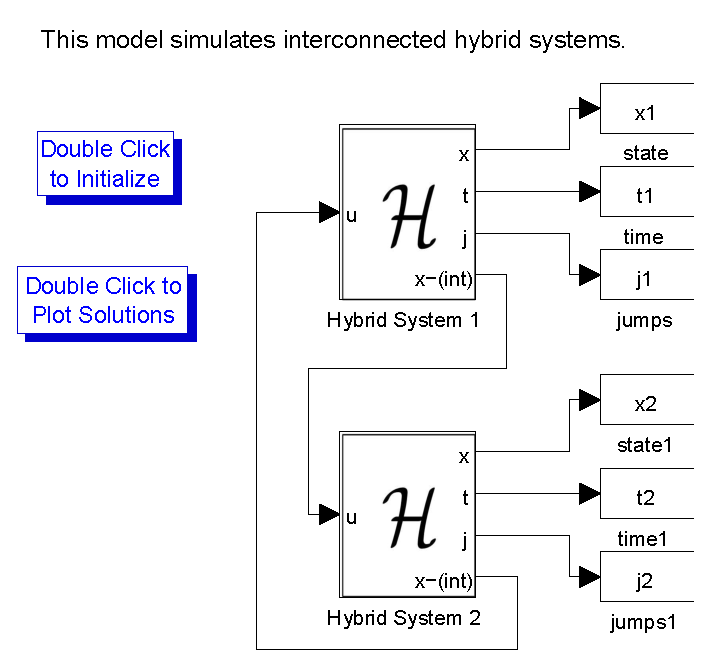
\includegraphics[width=.45\textwidth]{figures/Simulink/fireflies.eps}}
   \caption{Interconnection Diagram for Example~\ref{ex:fireflies}}
\label{fig:fireflies}
  \end{center}
\end{figure}
Each firefly can be modeled as a hybrid system given by
\begin{eqnarray}
f_i(\tau_i,u_i) & := & 1, \\
C_i &: =& \defset{(\tau_i,u_i)\in \Re^{2}}{0 \leq \tau_i \leq 1}\cap
\defset{(\tau_i,u_i)\in \Re^{2}}{0 \leq u_i \leq 1} \\
%\defset{(\tau_i,u_i)\in \Re^{2}}{(0 < \tau_i < 1), \cup (0 < u_i \leq 1)} \\
g_i(\tau_i,u_i) &:=&
\left\{
\begin{array}{ll}
(1+ \varepsilon)\tau_i
& (1+\varepsilon)\tau_i<1\\
0
& (1+\varepsilon)\tau_i\geq 1
\end{array}
\right. \\
    D_i &: =& \defset{(\tau_i,u_i)\in \Re^{2}}{\tau_i = 1} \cup \defset{(\tau_i,u_i)\in \Re^{2}}{u_i = 1}.
\end{eqnarray}
The interconnection diagram for this example is simpler than in the previous example because now no external inputs are being considered. The only event that affects the flashing of a firefly is the flashing of the other firefly. The interconnection diagram can be seen in Figure~\ref{fig:fireflies}.
%\ricardo{I removed the space between ``Figure'' and tilde you were putting
%as the reason of using a tilde is for "Figure" to stay together with the number (i.e., prevent hyphens due to spilling out a line.}

%\ricardo{Perhaps we should combine the figures below into subfigures so that they don't take
%so much space.  Perhaps two 1x2 grid of figures?}

\begin{figure}[ht]
  \psfrag{flows [t]}[c]{flows [$t$]}
  \psfrag{jumps [j]}[c]{jumps [$j$]}
  \psfrag{tau1}[c]{$\tau_1$}
  \psfrag{tau2}[c]{$\tau_2$}
  \centering
\subfigure[Solution for system $\HS_1$]{
    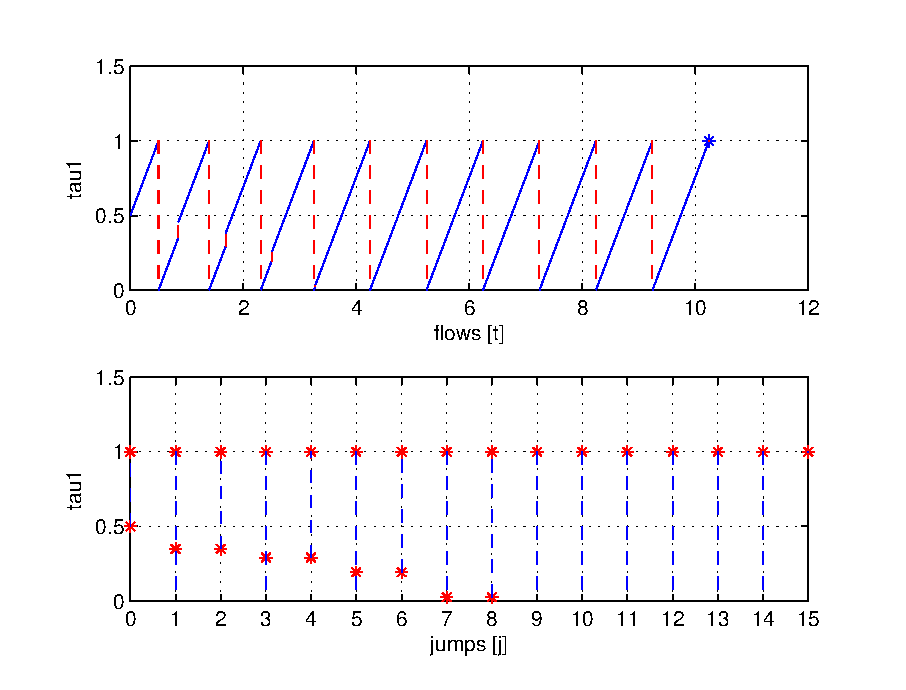
\includegraphics[width=0.45\textwidth]{figures/Examples/fireflyH1.eps}
\label{fig:fireflyH1}}
\qquad
\subfigure[Solution for system $\HS_2$]{
    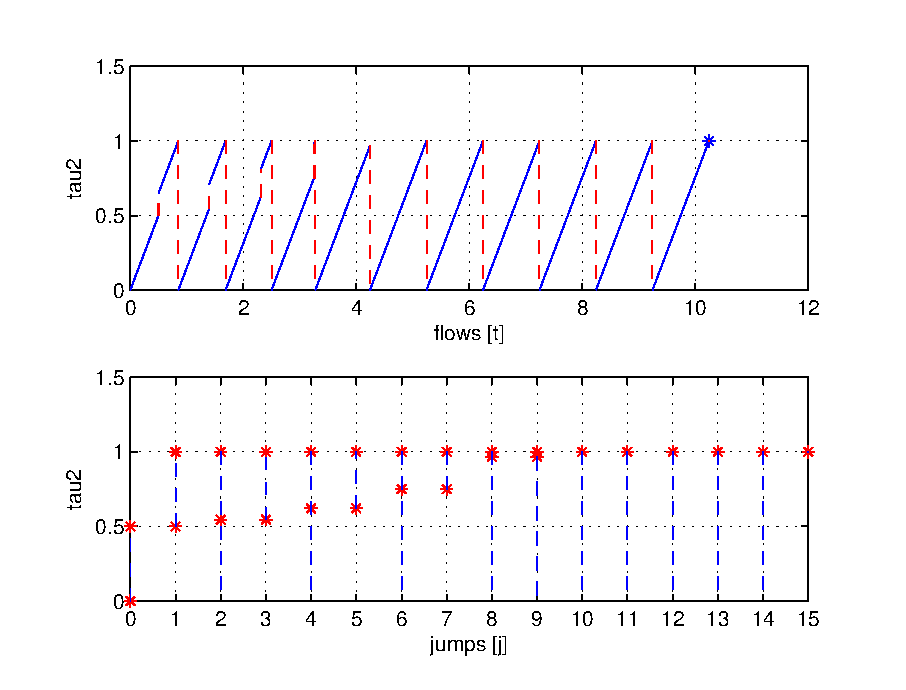
\includegraphics[width=0.45\textwidth]{figures/Examples/fireflyH2.eps}
\label{fig:fireflyH2}}
  \caption{Solution of Example \ref{ex:fireflies}}
\end{figure}

\begin{figure}[ht]
  \begin{center}
  \psfrag{flows [t]}[c]{flows [$t$]}
  \psfrag{jumps [j]}[c]{jumps [$j$]}
  \psfrag{tau1, tau2}[c]{$\tau_1, \tau_2$}
    {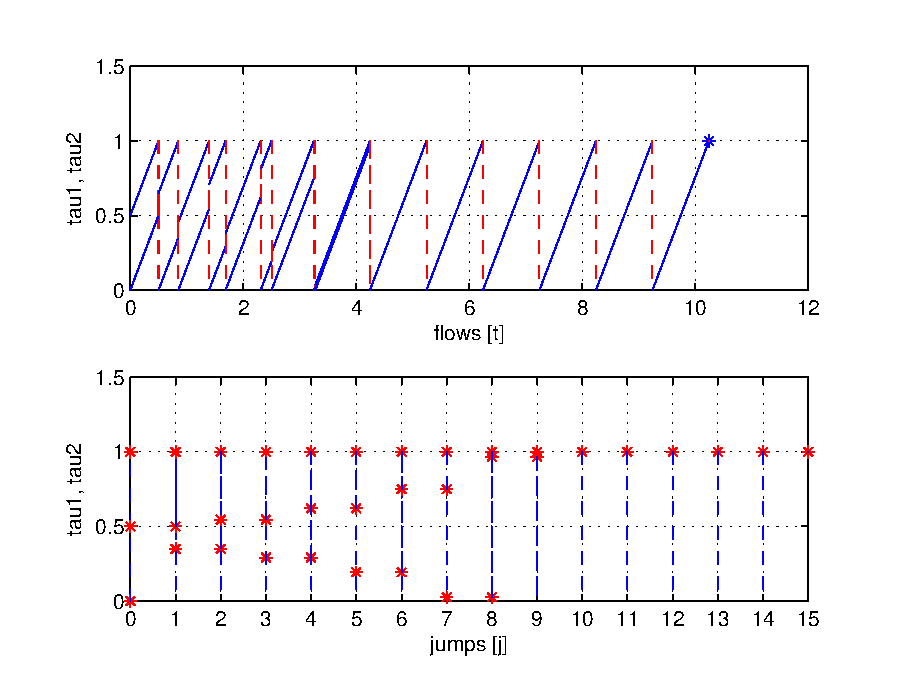
\includegraphics[width=.8\textwidth]{figures/Examples/fireflyH1H2.eps}}
   \caption{Solution of Example~\ref{ex:fireflies} for interconnection of $\HS_1$ and $\HS_2$}
\label{fig:fireflyH1H2}
  \end{center}
\end{figure}

For hybrid system $\HS_i$, $i = 1,2$:

Flow map
%\scriptsize
% This file was automatically created from the m-file 
% "m2tex.m" written by USL. 
% The fontencoding in this file is UTF-8. 
%  
% You will need to include the following two packages in 
% your LaTeX-Main-File. 
%  
% \usepackage{color} 
% \usepackage{fancyvrb} 
%  
% It is advised to use the following option for Inputenc 
% \usepackage[utf8]{inputenc} 
%  
  
% definition of matlab colors: 
\definecolor{mblue}{rgb}{0,0,1} 
\definecolor{mgreen}{rgb}{0.13333,0.5451,0.13333} 
\definecolor{mred}{rgb}{0.62745,0.12549,0.94118} 
\definecolor{mgrey}{rgb}{0.5,0.5,0.5} 
\definecolor{mdarkgrey}{rgb}{0.25,0.25,0.25} 
  
\DefineShortVerb[fontfamily=courier,fontseries=m]{\$} 
\DefineShortVerb[fontfamily=courier,fontseries=b]{\#} 
  
\noindent                    
 \hspace*{-1.6em}{\scriptsize 1}$  $\color{mblue}$function$\color{black}$ xdot = f(x, u, gamma)$\\
 \hspace*{-1.6em}{\scriptsize 2}$  $\\
 \hspace*{-1.6em}{\scriptsize 3}$  $\color{mgreen}#%%%%%%%%%%%%%%%%%%%%%%%%%%%%%%%%%%%%%%%%%%%%%%%%%%%%%%%%%%%%%%%%%%%%%%%%%%%#\color{black}$$\\
 \hspace*{-1.6em}{\scriptsize 4}$  $\color{mgreen}$% Matlab Function  Author: Ricardo Sanfelice $\color{black}$$\\
 \hspace*{-1.6em}{\scriptsize 5}$  $\color{mgreen}$% (Revised by Giampiero Campa)$\color{black}$$\\
 \hspace*{-1.6em}{\scriptsize 6}$  $\color{mgreen}$% (Revised by Pablo Nanez)$\color{black}$$\\
 \hspace*{-1.6em}{\scriptsize 7}$  $\color{mgreen}$%$\color{black}$$\\
 \hspace*{-1.6em}{\scriptsize 8}$  $\color{mgreen}$% Project: Simulation of a hybrid system (Bouncing Ball)$\color{black}$$\\
 \hspace*{-1.6em}{\scriptsize 9}$  $\color{mgreen}$%$\color{black}$$\\
 \hspace*{-2em}{\scriptsize 10}$  $\color{mgreen}$% Name: f.m$\color{black}$$\\
 \hspace*{-2em}{\scriptsize 11}$  $\color{mgreen}$%$\color{black}$$\\
 \hspace*{-2em}{\scriptsize 12}$  $\color{mgreen}$% Description: Flow map$\color{black}$$\\
 \hspace*{-2em}{\scriptsize 13}$  $\color{mgreen}$%$\color{black}$$\\
 \hspace*{-2em}{\scriptsize 14}$  $\color{mgreen}$% Version: 1.0$\color{black}$$\\
 \hspace*{-2em}{\scriptsize 15}$  $\color{mgreen}$% Required files: - $\color{black}$$\\
 \hspace*{-2em}{\scriptsize 16}$  $\color{mgreen}#%%%%%%%%%%%%%%%%%%%%%%%%%%%%%%%%%%%%%%%%%%%%%%%%%%%%%%%%%%%%%%%%%%%%%%%%%%%#\color{black}$$\\
 \hspace*{-2em}{\scriptsize 17}$  $\\
 \hspace*{-2em}{\scriptsize 18}$  $\\
 \hspace*{-2em}{\scriptsize 19}$  $\color{mgreen}$% flow map: xdot=f(x,u);$\color{black}$$\\
 \hspace*{-2em}{\scriptsize 20}$  xdot = [x(2); gamma];$\\ 
  
\UndefineShortVerb{\$} 
\UndefineShortVerb{\#}\label{scr:f}
%\normalsize

Flow set
%\scriptsize
% This file was automatically created from the m-file 
% "m2tex.m" written by USL. 
% The fontencoding in this file is UTF-8. 
%  
% You will need to include the following two packages in 
% your LaTeX-Main-File. 
%  
% \usepackage{color} 
% \usepackage{fancyvrb} 
%  
% It is advised to use the following option for Inputenc 
% \usepackage[utf8]{inputenc} 
%  
  
% definition of matlab colors: 
\definecolor{mblue}{rgb}{0,0,1} 
\definecolor{mgreen}{rgb}{0.13333,0.5451,0.13333} 
\definecolor{mred}{rgb}{0.62745,0.12549,0.94118} 
\definecolor{mgrey}{rgb}{0.5,0.5,0.5} 
\definecolor{mdarkgrey}{rgb}{0.25,0.25,0.25} 
  
\DefineShortVerb[fontfamily=courier,fontseries=m]{\$} 
\DefineShortVerb[fontfamily=courier,fontseries=b]{\#} 
  
\noindent                          
 \hspace*{-1.6em}{\scriptsize 1}$  $\color{mblue}$function$\color{black}$ v  = C(x, u)$\\
 \hspace*{-1.6em}{\scriptsize 2}$  $\color{mgreen}$%--------------------------------------------------------------------------$\color{black}$$\\
 \hspace*{-1.6em}{\scriptsize 3}$  $\color{mgreen}$% Matlab M-file Project: HyEQ Toolbox @  Hybrid Systems Laboratory (HSL),$\color{black}$$\\
 \hspace*{-1.6em}{\scriptsize 4}$  $\color{mgreen}$% https://hybrid.soe.ucsc.edu/software$\color{black}$$\\
 \hspace*{-1.6em}{\scriptsize 5}$  $\color{mgreen}$% http://hybridsimulator.wordpress.com/$\color{black}$$\\
 \hspace*{-1.6em}{\scriptsize 6}$  $\color{mgreen}$%--------------------------------------------------------------------------$\color{black}$$\\
 \hspace*{-1.6em}{\scriptsize 7}$  $\color{mgreen}$% Project: Simulation of a hybrid system$\color{black}$$\\
 \hspace*{-1.6em}{\scriptsize 8}$  $\color{mgreen}$% Description: Flow set$\color{black}$$\\
 \hspace*{-1.6em}{\scriptsize 9}$  $\color{mgreen}$%--------------------------------------------------------------------------$\color{black}$$\\
 \hspace*{-2em}{\scriptsize 10}$  $\color{mgreen}$%--------------------------------------------------------------------------$\color{black}$$\\
 \hspace*{-2em}{\scriptsize 11}$  $\color{mgreen}$%   See also HYEQSOLVER, PLOTARC, PLOTARC3, PLOTFLOWS, PLOTHARC,$\color{black}$$\\
 \hspace*{-2em}{\scriptsize 12}$  $\color{mgreen}$%   PLOTHARCCOLOR, PLOTHARCCOLOR3D, PLOTHYBRIDARC, PLOTJUMPS.$\color{black}$$\\
 \hspace*{-2em}{\scriptsize 13}$  $\color{mgreen}$%   Copyright @ Hybrid Systems Laboratory (HSL),$\color{black}$$\\
 \hspace*{-2em}{\scriptsize 14}$  $\color{mgreen}$%   Revision: 0.0.0.3 Date: 05/20/2015 3:42:00$\color{black}$$\\
 \hspace*{-2em}{\scriptsize 15}$  $\color{mgreen}$%$\color{black}$$\\
 \hspace*{-2em}{\scriptsize 16}$  $\color{mgreen}$% Check on flow conditions$\color{black}$$\\
 \hspace*{-2em}{\scriptsize 17}$  $\color{mgreen}$% E.g.,$\color{black}$$\\
 \hspace*{-2em}{\scriptsize 18}$  $\color{mgreen}$% if (x(1) >= u(1))  % flow condition$\color{black}$$\\
 \hspace*{-2em}{\scriptsize 19}$  $\color{mgreen}$%     v = 1;  % report flow$\color{black}$$\\
 \hspace*{-2em}{\scriptsize 20}$  $\color{mgreen}$% else$\color{black}$$\\
 \hspace*{-2em}{\scriptsize 21}$  $\color{mgreen}$%     v = 0;   % do not report flow$\color{black}$$\\
 \hspace*{-2em}{\scriptsize 22}$  $\color{mgreen}$% end$\color{black}$$\\
 \hspace*{-2em}{\scriptsize 23}$  $\\
 \hspace*{-2em}{\scriptsize 24}$  $\\
 \hspace*{-2em}{\scriptsize 25}$  v = 1; $\color{mgreen}$% report flow$\color{black}$$\\
 \hspace*{-2em}{\scriptsize 26}$  $\\ 
  
\UndefineShortVerb{\$} 
\UndefineShortVerb{\#}\label{scr:C}
%\normalsize

Jump map
%\scriptsize
% This file was automatically created from the m-file 
% "m2tex.m" written by USL. 
% The fontencoding in this file is UTF-8. 
%  
% You will need to include the following two packages in 
% your LaTeX-Main-File. 
%  
% \usepackage{color} 
% \usepackage{fancyvrb} 
%  
% It is advised to use the following option for Inputenc 
% \usepackage[utf8]{inputenc} 
%  
  
% definition of matlab colors: 
\definecolor{mblue}{rgb}{0,0,1} 
\definecolor{mgreen}{rgb}{0.13333,0.5451,0.13333} 
\definecolor{mred}{rgb}{0.62745,0.12549,0.94118} 
\definecolor{mgrey}{rgb}{0.5,0.5,0.5} 
\definecolor{mdarkgrey}{rgb}{0.25,0.25,0.25} 
  
\DefineShortVerb[fontfamily=courier,fontseries=m]{\$} 
\DefineShortVerb[fontfamily=courier,fontseries=b]{\#} 
  
\noindent   
 \hspace*{-1.6em}{\scriptsize 1}$  $\color{mblue}$function$\color{black}$ xplus = g(x, u, lambda)$\\
 \hspace*{-1.6em}{\scriptsize 2}$  $\color{mgreen}$% jump map$\color{black}$$\\
 \hspace*{-1.6em}{\scriptsize 3}$  xplus = [u(1); -lambda*x(2)];$\\ 
  
\UndefineShortVerb{\$} 
\UndefineShortVerb{\#}\label{scr:g}
%\normalsize

Jump set
%\scriptsize
% This file was automatically created from the m-file 
% "m2tex.m" written by USL. 
% The fontencoding in this file is UTF-8. 
%  
% You will need to include the following two packages in 
% your LaTeX-Main-File. 
%  
% \usepackage{color} 
% \usepackage{fancyvrb} 
%  
% It is advised to use the following option for Inputenc 
% \usepackage[utf8]{inputenc} 
%  
  
% definition of matlab colors: 
\definecolor{mblue}{rgb}{0,0,1} 
\definecolor{mgreen}{rgb}{0.13333,0.5451,0.13333} 
\definecolor{mred}{rgb}{0.62745,0.12549,0.94118} 
\definecolor{mgrey}{rgb}{0.5,0.5,0.5} 
\definecolor{mdarkgrey}{rgb}{0.25,0.25,0.25} 
  
\DefineShortVerb[fontfamily=courier,fontseries=m]{\$} 
\DefineShortVerb[fontfamily=courier,fontseries=b]{\#} 
  
\noindent                         
 \hspace*{-1.6em}{\scriptsize 1}$  $\color{mblue}$function$\color{black}$ v  = D(x, u) $\\
 \hspace*{-1.6em}{\scriptsize 2}$  $\\
 \hspace*{-1.6em}{\scriptsize 3}$  $\color{mgreen}#%%%%%%%%%%%%%%%%%%%%%%%%%%%%%%%%%%%%%%%%%%%%%%%%%%%%%%%%%%%%%%%%%%%%%%%%%%%#\color{black}$$\\
 \hspace*{-1.6em}{\scriptsize 4}$  $\color{mgreen}$% Matlab Function  Author: Ricardo Sanfelice $\color{black}$$\\
 \hspace*{-1.6em}{\scriptsize 5}$  $\color{mgreen}$% (Revised by Giampiero Campa)$\color{black}$$\\
 \hspace*{-1.6em}{\scriptsize 6}$  $\color{mgreen}$% (Revised by Pablo Nanez)$\color{black}$$\\
 \hspace*{-1.6em}{\scriptsize 7}$  $\color{mgreen}$%$\color{black}$$\\
 \hspace*{-1.6em}{\scriptsize 8}$  $\color{mgreen}$% Project: Simulation of a hybrid system (Bouncing ball)$\color{black}$$\\
 \hspace*{-1.6em}{\scriptsize 9}$  $\color{mgreen}$%$\color{black}$$\\
 \hspace*{-2em}{\scriptsize 10}$  $\color{mgreen}$% Name: D.m$\color{black}$$\\
 \hspace*{-2em}{\scriptsize 11}$  $\color{mgreen}$%$\color{black}$$\\
 \hspace*{-2em}{\scriptsize 12}$  $\color{mgreen}$% Description: Jump set$\color{black}$$\\
 \hspace*{-2em}{\scriptsize 13}$  $\color{mgreen}$%$\color{black}$$\\
 \hspace*{-2em}{\scriptsize 14}$  $\color{mgreen}$% Version: 1.0$\color{black}$$\\
 \hspace*{-2em}{\scriptsize 15}$  $\color{mgreen}$% Required files: - $\color{black}$$\\
 \hspace*{-2em}{\scriptsize 16}$  $\color{mgreen}#%%%%%%%%%%%%%%%%%%%%%%%%%%%%%%%%%%%%%%%%%%%%%%%%%%%%%%%%%%%%%%%%%%%%%%%%%%%#\color{black}$$\\
 \hspace*{-2em}{\scriptsize 17}$  $\\
 \hspace*{-2em}{\scriptsize 18}$  xtemp = zeros(2,1);$\\
 \hspace*{-2em}{\scriptsize 19}$  xtemp = x;$\\
 \hspace*{-2em}{\scriptsize 20}$  $\\
 \hspace*{-2em}{\scriptsize 21}$  $\color{mblue}$if$\color{black}$ (xtemp(1) <= u(1)) && (xtemp(2) <= 0)  $\color{mgreen}$% jump condition$\color{black}$$\\
 \hspace*{-2em}{\scriptsize 22}$      v = 1;  $\color{mgreen}$% report jump$\color{black}$$\\
 \hspace*{-2em}{\scriptsize 23}$  $\color{mblue}$else$\color{black}$$\\
 \hspace*{-2em}{\scriptsize 24}$      v = 0;   $\color{mgreen}$% do not report jump$\color{black}$$\\
 \hspace*{-2em}{\scriptsize 25}$  $\color{mblue}$end$\color{black}$$\\ 
  
\UndefineShortVerb{\$} 
\UndefineShortVerb{\#}\label{scr:D}
%\normalsize

A solution to the interconnection of hybrid systems $\HS_1$ and
$\HS_2$ with $T=15, J=15$, $rule =1$, $\varepsilon=0.3$ is depicted in Figure~\ref{fig:fireflyH1H2}. Both the projection onto $t$ and $j$ are shown. A solution to the hybrid system $\HS_1$ is depicted in Figure~\ref{fig:fireflyH1}. A solution to the hybrid system $\HS_2$ is depicted in Figure~\ref{fig:fireflyH2}.

These simulations reflect the expected behavior of the interconnected hybrid systems. The fireflies initially flash out of phase with one another and then synchronize to flash in the same phase.

For MATLAB/Simulink files of this example, see \IfSAE{Examples/Example\_\ref{ex:fireflies}}{Examples/Example\_1.7}.

\end{example}





% 
\begin{example}{a simple mathematical example to show different type of simulation results}
\label{ex:overlap1}
Consider the hybrid system with data
\begin{eqnarray*}
f(x) := -x,\ C:= [0,1], \
g(x) := 1+\mbox{mod}(x,2), \ D:=  \{1\}\cup\{2\}.
\end{eqnarray*}

Note that solutions from $\solinit = 1$ and $\solinit = 2$ are
nonunique.  The following simulations show the use of the variable
$rule$ in the {\em Jump Logic block}.
% show forcing logic

{\bf Jumps enforced:}
A solution from $x0=1$ with $T=10,J=20$, $rule = 1$ is depicted in
Figure~\ref{fig:overlap1-1}. The solution jumps from $1$ to
$2$, and from $2$ to $1$ repetitively.

{\bf Flows enforced:}
A solution from $x0=1$ with $T=10,J=20$, $rule = 2$ is depicted in
Figure~\ref{fig:overlap1-2}. The solution flows for all time
and converges exponentially to zero.

\begin{figure}[ht]
\begin{center}
\subfigure[Forced jumps logic. \label{fig:overlap1-1}]
{
\psfragfig[width=.45\textwidth]{figures/Examples/Overlap1JumpPriority}
{
  \psfrag{flows [t]}[c]{flows [$t$]}
  \psfrag{jumps [j]}[c]{jumps [$j$]}
  \psfrag{x}[c]{$x$}
}
}
\qquad
\subfigure[Forced flows logic. \label{fig:overlap1-2}]
{
    \psfragfig[width=.45\textwidth]{figures/Examples/Overlap1FlowPriority}
{
  \psfrag{flows [t]}[c]{flows [$t$]}
  \psfrag{jumps [j]}[c]{jumps [$j$]}
  \psfrag{x}[c]{$x$}
}
}
\end{center}
\caption{Solution of Example~\ref{ex:overlap1}}
\end{figure}

\begin{figure}[ht]
  \psfrag{flows [t]}[c]{flows [$t$]}
  \psfrag{jumps [j]}[c]{jumps [$j$]}
  \psfrag{x}[c]{$x$}
  \centering
\subfigure[Random logic for flowing/jumping.]{
    \includegraphics[width=.45\textwidth]{figures/Examples/Overlap1RandomPriority.eps}
\label{fig:overlap1-3}}
\subfigure[Random logic for flowing/jumping.]{
    \includegraphics[width=.45\textwidth]{figures/Examples/Overlap1TRandomPriority.eps}
\label{fig:overlap1T-1}}
\qquad
\subfigure[Random logic for flowing/jumping. Zoomed version.]{
    \includegraphics[width=.45\textwidth]{figures/Examples/Overlap1TRandomPriorityZoom.eps}
\label{fig:overlap1T-2}}
\caption{Solution of Example~\ref{ex:overlap1}}
\end{figure}

{\bf Random rule:}
A solution from $x0=1$ with $T=10,J=20$, $rule = 3$ is depicted in
Figure~\ref{fig:overlap1-3}. The solution jumps to $2$, then jumps to
$1$ and flows for the rest of the time converging to zero
exponentially.
Enlarging $D$ to
\begin{eqnarray*}
D:=  [1/50,1]\cup\{2\}
\end{eqnarray*}
causes the overlap between $C$ and $D$ to be ``thicker''.
The simulation result is
depicted in Figure~\ref{fig:overlap1T-1}
with the same parameters used in the simulation in
Figure~\ref{fig:overlap1-3}.
The plot suggests that the solution jumps several times until
$x<1/50$ from where it flows to zero.  However,
Figure~\ref{fig:overlap1T-2},
a zoomed version of Figure~\ref{fig:overlap1T-1},
shows that initially the
solution flows and that at $(t,j)=(0.2 e-3,0)$ it jumps. After the jump,
it continues flowing, then it jumps a few times, then it flows, etc.
The combination of flowing and jumping occurs while the solution
is in the intersection of $C$ and $D$, where the selection
of whether flowing or jumping is done randomly due to using $rule=3$.

This simulation also reveals that this implementation does not
precisely generate hybrid arcs. The maximum step size was set to $0.1
e-3$. The solution flows during the first two steps of the integration
of the flows with maximum step size. The value at $t=0.1e-3$ is very
close to $1$. At $t=0.2e-3$, instead of assuming a value given by the
flow map, the value of the solution is about $0.5$, which is the
result of the jump occurring at $(0.2e-3,0)$. This is the value stored
in $x$ at such time by the integrator. Note that the value of $x'$ at
$(0.2e-3,0)$ is the one given by the flow map that triggers the jump,
and if available for recording, it should be stored in $(0.2e-3,0)$.
This is a limitation of the current implementation.

The following simulations show the {\em Stop Logic block} stopping
the simulation at different events.
\begin{figure}[ht]
  \centering
  \psfrag{flows [t]}[c]{flows [$t$]}
  \psfrag{jumps [j]}[c]{jumps [$j$]}
  \psfrag{x}[c]{$x$}
\subfigure[Forced jump logic and different $D$.]{
    \includegraphics[width=.45\textwidth]{figures/Examples/Overlap2JumpPriority.eps}
\label{fig:overlap2-1}}
\qquad
\subfigure[Forced flow logic.]{
    \includegraphics[width=.45\textwidth]{figures/Examples/Overlap4FlowPriority.eps}
\label{fig:overlap4-1}}
\caption{Solution of Example~\ref{ex:overlap1} with premature stopping.}
\end{figure}

{\bf Solution outside $C\cup D$:}
Taking $D = \{1\}$, a simulation starting from $x0=1$ with $T=10,J=20$, $rule = 1$ stops since the solution leaves $C\cup D$. Figure~\ref{fig:overlap2-1} shows this.

% show stopping logic by C
{\bf Solution reaches the boundary of $C$ from where jumps are not possible:}
Replacing the flow set by  $[1/2,1]$
a solution starting from $x0=1$ with $T=10,J=20$ and $rule = 2$
flows for all time until it reaches the boundary of
$C$ where jumps are not possible. Figure~\ref{fig:overlap4-1}
shows this.

Note that in this implementation, the Stop Logic is such that when the
state of the hybrid system is not in $(C \cup D)$, then the
simulation is stopped. In particular, if this condition becomes true
while flowing, then the last value of the computed solution will not
belong to $C$. It
could be desired to be able to recompute the solution so that its last
point belongs to the corresponding set. From that point, it should be
the case that solutions cannot be continued.

For MATLAB/Simulink files of this example, see \IfSAE{Examples/Example\_\ref{ex:overlap1}}{Examples/Example\_1.8}.

\end{example}





% \begin{example}{Linear time-invariant plant}
\label{ex:LTIplant}

Following the model of a physical component 
\IfSAE
{
\begin{subequations}\label{eqn:CPSplant}
\begin{align}
\dot{x} &= f(x,u), 
&C &:= \{ x\ |\ x \in \Re^{n}\},\\
\x^+ &= g(x) =\emptyset,
&D &:= \emptyset,\\
y &= h(x,u)
\end{align}
\end{subequations}
}
{
in~\eqref{eqn:CPSplant},
} 
a linear time-invariant model of the physical component is defined by
$$
f(\xp,\up) = \fp(\xp,\up)= A_P \xp + B_P \up, \qquad h(\xp,\up) = \hp(\xp,\up) = M_P \xp + N_P \up
$$
where $A_P$, $B_P$, $M_P$, and $N_P$ are matrices of appropriate dimensions. 
State and input constraints can directly be embedded into the set $\Cp$. 
For example, the constraint that $\xp$ has all of its components 
nonnegative and that $\up$ has its components with norm
less or equal than one is captured by 
\begin{eqnarray*}
C_P &=& \defset{(\xp,\up)\in\reals^{n_P}\times \reals^{m_P}}{\xp_i \geq 0 \ \forall i \in \{1,2,\ldots,n_P\}} 
\\ & & \qquad \cap \defset{(\xp,\up)\in\reals^{n_P}\times \reals^{m_P}}{|\up_i| \leq 1 \  \forall i \in \{1,2,\ldots,m_P\}}
\end{eqnarray*}
For example, the evolution of the temperature of a room with a heater
can be modeled by a linear-time invariant system 
with state $\xp$ denoting the temperature of the room
and with input $\up = (\up_1,\up_2)$, where 
$\up_1$ denotes whether the heater is turned on ($\up_1 = 1$) or
turned off ($\up_1 = 0$) while $\up_2$ denotes the temperature
outside the room.
The evolution of the temperature is given by
\begin{eqnarray}\label{eqn:TemperatureModel}
\xpdot & = & -\xp + \matt{z_\Delta & 1} \matt{\up_1 \\ \up_2} \qquad \mbox{ when } (\xp,\up)\in \Cp= \defset{(\xp,\up) \in \reals\times\reals^2}{\up_1 \in \{0,1\}}
\end{eqnarray}
where $z_\Delta$ is a constant representing the heater capacity.
\end{example}


% \begin{example}{Implementation of a FSM}\label{ex:FSM}

\begin{figure}
  \begin{center}
    {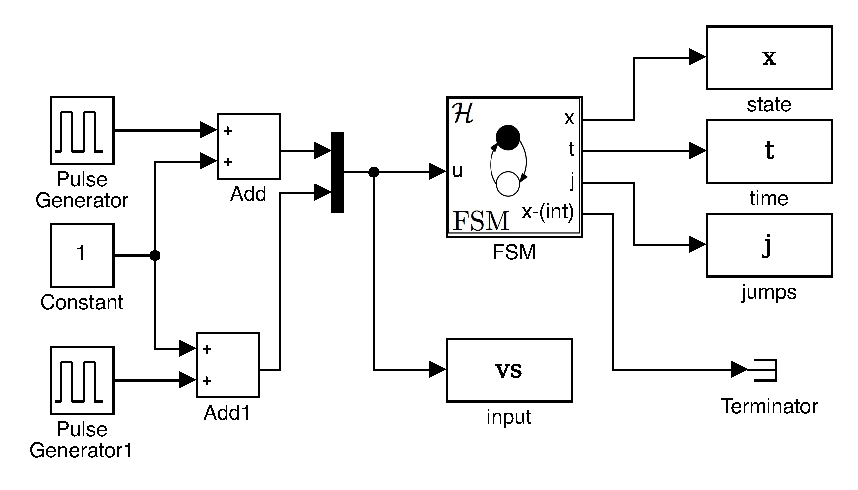
\includegraphics[width=0.6\textwidth]{figures/Simulink/FSM_example.eps}}
   \caption{Simulation of a Finite State Machine (FSM) in Example~\ref{ex:FSM}.}
\label{fig:FSM_example}
  \end{center}
\end{figure}

Transitions of the state of a FSM are triggered by changes of its input $\uc$.
The system can be modeled as a cascade of two systems,
in which an external signal drives the FSM. 
\IfSAE
{
A finite state machine (FSM) or deterministic finite automaton (DFA) is a system with
inputs, states, and outputs taking values from discrete sets that are updated at discrete transitions (or jumps)
triggered by its inputs. 
Then, given a FSM and an initial state $\xlogic_0 \in \xlogicSpace$,  
a transition to a state $\xlogic_1 = \delta(\xlogic_0,\uc)$ is performed
when an input $\uc \in \Sigma$ is applied to it.
After the transition, the output of the FSM is updated to $\hc(\xlogic_1)$.
This mechanism can be captured by the difference equation
\begin{eqnarray}\label{eqn:FSMmodel}
\xlogic^+ & = & \delta(\xlogic,\uc)  \qquad \yc \ = \ \hc(\xlogic) \qquad (\xlogic,\uc)  \in \xlogicSpace \times \Sigma
\end{eqnarray}
This model captures the dynamics
the model of the cyber components 
in the instructions document
with
$$
\xc = \xlogic, \qquad \xcSpace = \xlogicSpace, \qquad \ucSpace = \Sigma, \qquad \gc = \delta, \qquad \Dc = \xcSpace\times\ucSpace
$$
Note that there is no notion of time associated with the FSM model above. An example of this model is presented in Example~\ref{ex:FSM}. 
}
{The FSM is modeled as the difference equation in \eqref{eqn:FSMmodel}.}
Assuming that the input feeds the input $u$ of the FSM, 
the state of the FSM is updated according to the transition function evaluated at the current input, that is,
$\xlogic$ is updated according to
 $$
\xlogic^+  =  \delta(\xlogic,u)
$$

The above model can be summarized as follows:

\begin{align}\label{eqn:CTdynamicsHcFSM}
f(\xlogic, u)&:= \begin{bmatrix}0\\0\end{bmatrix},\\ 
   C :=& \defset{(\xlogic,u)\in\{1,2\}\times\{1,2\}\times\{1,2\}\times\{1,2\}}{ \delta(\xlogic,u) =  \xlogic},\\
g(\xlogic, u)&:= \delta(\xlogic, u) = \begin{bmatrix}3-u_1\\3-u_2\end{bmatrix}, \\
    D :=& \defset{(\xlogic,u)\in\{1,2\}\times\{1,2\}\times\{1,2\}\times\{1,2\}}{ \delta(\xlogic,u) \in\{1,2\}\times\{1,2\}\setminus \xlogic},\\ 
y &:= h(\xlogic) =\xlogic
\end{align}
where the input and the state are given by $u = (u_1,u_2) \in\{1,2\}\times\{1,2\}$, and $\xlogic=(\xlogic_1,\xlogic_2)\in\{1,2\}\times\{1,2\}$, respectively.

For the hybrid system FSM in Figure~\ref{fig:FSM_example} we have the following Matlab embedded functions that describe the sets $C$ and $D$ and functions $f$ and $g$.
Figure~\ref{fig:FSMresults} depicts the corresponding inputs and state of the FSM.

\begin{figure}[ht]
  \begin{center}
    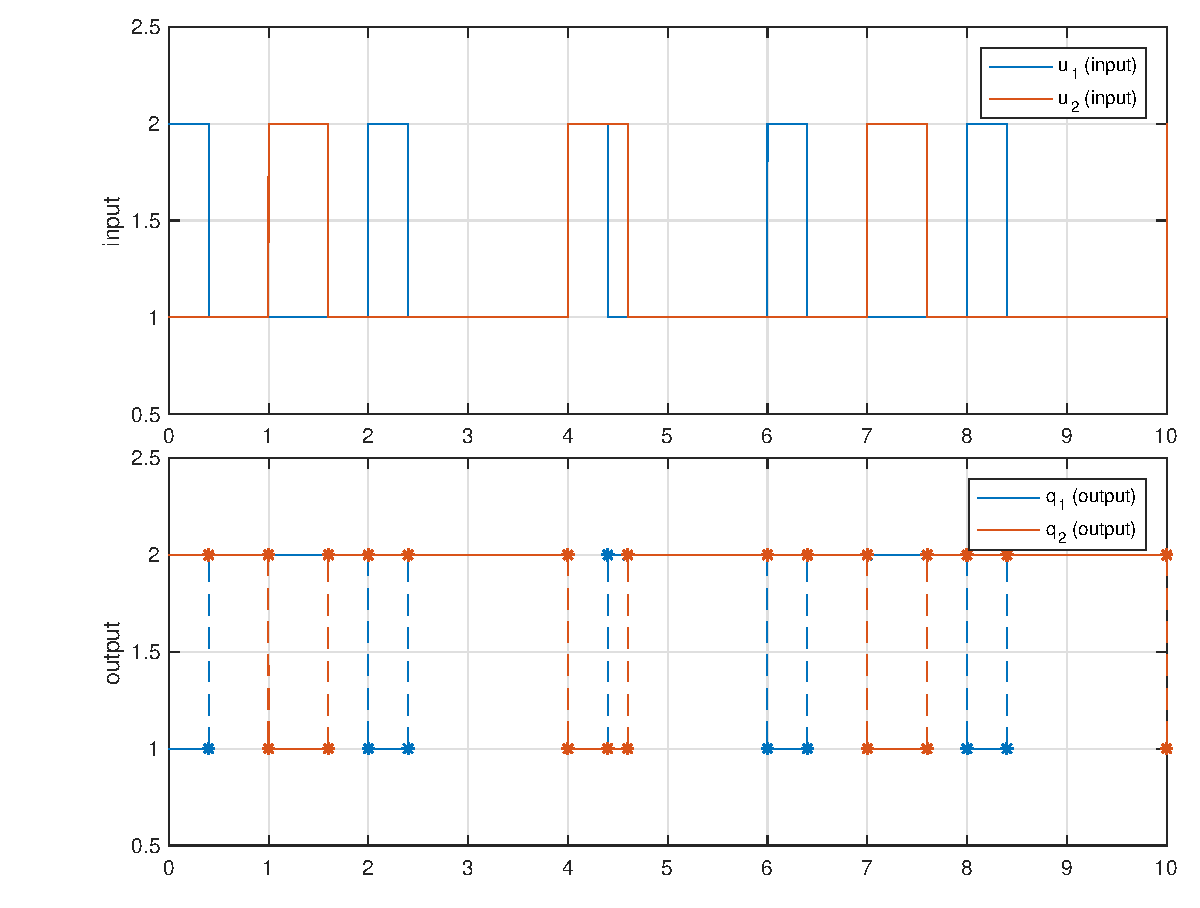
\includegraphics[width=0.8\textwidth]{figures/Simulink/FSMresults.eps}
   \caption{Finite state machine states and inputs.}
\label{fig:FSMresults}
  \end{center}
\end{figure}

% Set the location for MATLAB files included via the "\code" command.
\codeLocation{Matlab2tex_FSM}

\code{f.m}
\code{C.m}
\code{g.m}
\code{D.m}

% Flow map
% %\scriptsize
% % This file was automatically created from the m-file 
% "m2tex.m" written by USL. 
% The fontencoding in this file is UTF-8. 
%  
% You will need to include the following two packages in 
% your LaTeX-Main-File. 
%  
% \usepackage{color} 
% \usepackage{fancyvrb} 
%  
% It is advised to use the following option for Inputenc 
% \usepackage[utf8]{inputenc} 
%  
  
% definition of matlab colors: 
\definecolor{mblue}{rgb}{0,0,1} 
\definecolor{mgreen}{rgb}{0.13333,0.5451,0.13333} 
\definecolor{mred}{rgb}{0.62745,0.12549,0.94118} 
\definecolor{mgrey}{rgb}{0.5,0.5,0.5} 
\definecolor{mdarkgrey}{rgb}{0.25,0.25,0.25} 
  
\DefineShortVerb[fontfamily=courier,fontseries=m]{\$} 
\DefineShortVerb[fontfamily=courier,fontseries=b]{\#} 
  
\noindent                    
 \hspace*{-1.6em}{\scriptsize 1}$  $\color{mblue}$function$\color{black}$ xdot = f(x, u, gamma)$\\
 \hspace*{-1.6em}{\scriptsize 2}$  $\\
 \hspace*{-1.6em}{\scriptsize 3}$  $\color{mgreen}#%%%%%%%%%%%%%%%%%%%%%%%%%%%%%%%%%%%%%%%%%%%%%%%%%%%%%%%%%%%%%%%%%%%%%%%%%%%#\color{black}$$\\
 \hspace*{-1.6em}{\scriptsize 4}$  $\color{mgreen}$% Matlab Function  Author: Ricardo Sanfelice $\color{black}$$\\
 \hspace*{-1.6em}{\scriptsize 5}$  $\color{mgreen}$% (Revised by Giampiero Campa)$\color{black}$$\\
 \hspace*{-1.6em}{\scriptsize 6}$  $\color{mgreen}$% (Revised by Pablo Nanez)$\color{black}$$\\
 \hspace*{-1.6em}{\scriptsize 7}$  $\color{mgreen}$%$\color{black}$$\\
 \hspace*{-1.6em}{\scriptsize 8}$  $\color{mgreen}$% Project: Simulation of a hybrid system (Bouncing Ball)$\color{black}$$\\
 \hspace*{-1.6em}{\scriptsize 9}$  $\color{mgreen}$%$\color{black}$$\\
 \hspace*{-2em}{\scriptsize 10}$  $\color{mgreen}$% Name: f.m$\color{black}$$\\
 \hspace*{-2em}{\scriptsize 11}$  $\color{mgreen}$%$\color{black}$$\\
 \hspace*{-2em}{\scriptsize 12}$  $\color{mgreen}$% Description: Flow map$\color{black}$$\\
 \hspace*{-2em}{\scriptsize 13}$  $\color{mgreen}$%$\color{black}$$\\
 \hspace*{-2em}{\scriptsize 14}$  $\color{mgreen}$% Version: 1.0$\color{black}$$\\
 \hspace*{-2em}{\scriptsize 15}$  $\color{mgreen}$% Required files: - $\color{black}$$\\
 \hspace*{-2em}{\scriptsize 16}$  $\color{mgreen}#%%%%%%%%%%%%%%%%%%%%%%%%%%%%%%%%%%%%%%%%%%%%%%%%%%%%%%%%%%%%%%%%%%%%%%%%%%%#\color{black}$$\\
 \hspace*{-2em}{\scriptsize 17}$  $\\
 \hspace*{-2em}{\scriptsize 18}$  $\\
 \hspace*{-2em}{\scriptsize 19}$  $\color{mgreen}$% flow map: xdot=f(x,u);$\color{black}$$\\
 \hspace*{-2em}{\scriptsize 20}$  xdot = [x(2); gamma];$\\ 
  
\UndefineShortVerb{\$} 
\UndefineShortVerb{\#}\label{scr:f}
% %\normalsize

% Flow set
% %\scriptsize
% % This file was automatically created from the m-file 
% "m2tex.m" written by USL. 
% The fontencoding in this file is UTF-8. 
%  
% You will need to include the following two packages in 
% your LaTeX-Main-File. 
%  
% \usepackage{color} 
% \usepackage{fancyvrb} 
%  
% It is advised to use the following option for Inputenc 
% \usepackage[utf8]{inputenc} 
%  
  
% definition of matlab colors: 
\definecolor{mblue}{rgb}{0,0,1} 
\definecolor{mgreen}{rgb}{0.13333,0.5451,0.13333} 
\definecolor{mred}{rgb}{0.62745,0.12549,0.94118} 
\definecolor{mgrey}{rgb}{0.5,0.5,0.5} 
\definecolor{mdarkgrey}{rgb}{0.25,0.25,0.25} 
  
\DefineShortVerb[fontfamily=courier,fontseries=m]{\$} 
\DefineShortVerb[fontfamily=courier,fontseries=b]{\#} 
  
\noindent                          
 \hspace*{-1.6em}{\scriptsize 1}$  $\color{mblue}$function$\color{black}$ v  = C(x, u)$\\
 \hspace*{-1.6em}{\scriptsize 2}$  $\color{mgreen}$%--------------------------------------------------------------------------$\color{black}$$\\
 \hspace*{-1.6em}{\scriptsize 3}$  $\color{mgreen}$% Matlab M-file Project: HyEQ Toolbox @  Hybrid Systems Laboratory (HSL),$\color{black}$$\\
 \hspace*{-1.6em}{\scriptsize 4}$  $\color{mgreen}$% https://hybrid.soe.ucsc.edu/software$\color{black}$$\\
 \hspace*{-1.6em}{\scriptsize 5}$  $\color{mgreen}$% http://hybridsimulator.wordpress.com/$\color{black}$$\\
 \hspace*{-1.6em}{\scriptsize 6}$  $\color{mgreen}$%--------------------------------------------------------------------------$\color{black}$$\\
 \hspace*{-1.6em}{\scriptsize 7}$  $\color{mgreen}$% Project: Simulation of a hybrid system$\color{black}$$\\
 \hspace*{-1.6em}{\scriptsize 8}$  $\color{mgreen}$% Description: Flow set$\color{black}$$\\
 \hspace*{-1.6em}{\scriptsize 9}$  $\color{mgreen}$%--------------------------------------------------------------------------$\color{black}$$\\
 \hspace*{-2em}{\scriptsize 10}$  $\color{mgreen}$%--------------------------------------------------------------------------$\color{black}$$\\
 \hspace*{-2em}{\scriptsize 11}$  $\color{mgreen}$%   See also HYEQSOLVER, PLOTARC, PLOTARC3, PLOTFLOWS, PLOTHARC,$\color{black}$$\\
 \hspace*{-2em}{\scriptsize 12}$  $\color{mgreen}$%   PLOTHARCCOLOR, PLOTHARCCOLOR3D, PLOTHYBRIDARC, PLOTJUMPS.$\color{black}$$\\
 \hspace*{-2em}{\scriptsize 13}$  $\color{mgreen}$%   Copyright @ Hybrid Systems Laboratory (HSL),$\color{black}$$\\
 \hspace*{-2em}{\scriptsize 14}$  $\color{mgreen}$%   Revision: 0.0.0.3 Date: 05/20/2015 3:42:00$\color{black}$$\\
 \hspace*{-2em}{\scriptsize 15}$  $\color{mgreen}$%$\color{black}$$\\
 \hspace*{-2em}{\scriptsize 16}$  $\color{mgreen}$% Check on flow conditions$\color{black}$$\\
 \hspace*{-2em}{\scriptsize 17}$  $\color{mgreen}$% E.g.,$\color{black}$$\\
 \hspace*{-2em}{\scriptsize 18}$  $\color{mgreen}$% if (x(1) >= u(1))  % flow condition$\color{black}$$\\
 \hspace*{-2em}{\scriptsize 19}$  $\color{mgreen}$%     v = 1;  % report flow$\color{black}$$\\
 \hspace*{-2em}{\scriptsize 20}$  $\color{mgreen}$% else$\color{black}$$\\
 \hspace*{-2em}{\scriptsize 21}$  $\color{mgreen}$%     v = 0;   % do not report flow$\color{black}$$\\
 \hspace*{-2em}{\scriptsize 22}$  $\color{mgreen}$% end$\color{black}$$\\
 \hspace*{-2em}{\scriptsize 23}$  $\\
 \hspace*{-2em}{\scriptsize 24}$  $\\
 \hspace*{-2em}{\scriptsize 25}$  v = 1; $\color{mgreen}$% report flow$\color{black}$$\\
 \hspace*{-2em}{\scriptsize 26}$  $\\ 
  
\UndefineShortVerb{\$} 
\UndefineShortVerb{\#}\label{scr:C}
% %\normalsize

% Jump map
% %\scriptsize
% % This file was automatically created from the m-file 
% "m2tex.m" written by USL. 
% The fontencoding in this file is UTF-8. 
%  
% You will need to include the following two packages in 
% your LaTeX-Main-File. 
%  
% \usepackage{color} 
% \usepackage{fancyvrb} 
%  
% It is advised to use the following option for Inputenc 
% \usepackage[utf8]{inputenc} 
%  
  
% definition of matlab colors: 
\definecolor{mblue}{rgb}{0,0,1} 
\definecolor{mgreen}{rgb}{0.13333,0.5451,0.13333} 
\definecolor{mred}{rgb}{0.62745,0.12549,0.94118} 
\definecolor{mgrey}{rgb}{0.5,0.5,0.5} 
\definecolor{mdarkgrey}{rgb}{0.25,0.25,0.25} 
  
\DefineShortVerb[fontfamily=courier,fontseries=m]{\$} 
\DefineShortVerb[fontfamily=courier,fontseries=b]{\#} 
  
\noindent   
 \hspace*{-1.6em}{\scriptsize 1}$  $\color{mblue}$function$\color{black}$ xplus = g(x, u, lambda)$\\
 \hspace*{-1.6em}{\scriptsize 2}$  $\color{mgreen}$% jump map$\color{black}$$\\
 \hspace*{-1.6em}{\scriptsize 3}$  xplus = [u(1); -lambda*x(2)];$\\ 
  
\UndefineShortVerb{\$} 
\UndefineShortVerb{\#}\label{scr:g}
% %\normalsize

% Jump set
% %\scriptsize
% % This file was automatically created from the m-file 
% "m2tex.m" written by USL. 
% The fontencoding in this file is UTF-8. 
%  
% You will need to include the following two packages in 
% your LaTeX-Main-File. 
%  
% \usepackage{color} 
% \usepackage{fancyvrb} 
%  
% It is advised to use the following option for Inputenc 
% \usepackage[utf8]{inputenc} 
%  
  
% definition of matlab colors: 
\definecolor{mblue}{rgb}{0,0,1} 
\definecolor{mgreen}{rgb}{0.13333,0.5451,0.13333} 
\definecolor{mred}{rgb}{0.62745,0.12549,0.94118} 
\definecolor{mgrey}{rgb}{0.5,0.5,0.5} 
\definecolor{mdarkgrey}{rgb}{0.25,0.25,0.25} 
  
\DefineShortVerb[fontfamily=courier,fontseries=m]{\$} 
\DefineShortVerb[fontfamily=courier,fontseries=b]{\#} 
  
\noindent                         
 \hspace*{-1.6em}{\scriptsize 1}$  $\color{mblue}$function$\color{black}$ v  = D(x, u) $\\
 \hspace*{-1.6em}{\scriptsize 2}$  $\\
 \hspace*{-1.6em}{\scriptsize 3}$  $\color{mgreen}#%%%%%%%%%%%%%%%%%%%%%%%%%%%%%%%%%%%%%%%%%%%%%%%%%%%%%%%%%%%%%%%%%%%%%%%%%%%#\color{black}$$\\
 \hspace*{-1.6em}{\scriptsize 4}$  $\color{mgreen}$% Matlab Function  Author: Ricardo Sanfelice $\color{black}$$\\
 \hspace*{-1.6em}{\scriptsize 5}$  $\color{mgreen}$% (Revised by Giampiero Campa)$\color{black}$$\\
 \hspace*{-1.6em}{\scriptsize 6}$  $\color{mgreen}$% (Revised by Pablo Nanez)$\color{black}$$\\
 \hspace*{-1.6em}{\scriptsize 7}$  $\color{mgreen}$%$\color{black}$$\\
 \hspace*{-1.6em}{\scriptsize 8}$  $\color{mgreen}$% Project: Simulation of a hybrid system (Bouncing ball)$\color{black}$$\\
 \hspace*{-1.6em}{\scriptsize 9}$  $\color{mgreen}$%$\color{black}$$\\
 \hspace*{-2em}{\scriptsize 10}$  $\color{mgreen}$% Name: D.m$\color{black}$$\\
 \hspace*{-2em}{\scriptsize 11}$  $\color{mgreen}$%$\color{black}$$\\
 \hspace*{-2em}{\scriptsize 12}$  $\color{mgreen}$% Description: Jump set$\color{black}$$\\
 \hspace*{-2em}{\scriptsize 13}$  $\color{mgreen}$%$\color{black}$$\\
 \hspace*{-2em}{\scriptsize 14}$  $\color{mgreen}$% Version: 1.0$\color{black}$$\\
 \hspace*{-2em}{\scriptsize 15}$  $\color{mgreen}$% Required files: - $\color{black}$$\\
 \hspace*{-2em}{\scriptsize 16}$  $\color{mgreen}#%%%%%%%%%%%%%%%%%%%%%%%%%%%%%%%%%%%%%%%%%%%%%%%%%%%%%%%%%%%%%%%%%%%%%%%%%%%#\color{black}$$\\
 \hspace*{-2em}{\scriptsize 17}$  $\\
 \hspace*{-2em}{\scriptsize 18}$  xtemp = zeros(2,1);$\\
 \hspace*{-2em}{\scriptsize 19}$  xtemp = x;$\\
 \hspace*{-2em}{\scriptsize 20}$  $\\
 \hspace*{-2em}{\scriptsize 21}$  $\color{mblue}$if$\color{black}$ (xtemp(1) <= u(1)) && (xtemp(2) <= 0)  $\color{mgreen}$% jump condition$\color{black}$$\\
 \hspace*{-2em}{\scriptsize 22}$      v = 1;  $\color{mgreen}$% report jump$\color{black}$$\\
 \hspace*{-2em}{\scriptsize 23}$  $\color{mblue}$else$\color{black}$$\\
 \hspace*{-2em}{\scriptsize 24}$      v = 0;   $\color{mgreen}$% do not report jump$\color{black}$$\\
 \hspace*{-2em}{\scriptsize 25}$  $\color{mblue}$end$\color{black}$$\\ 
  
\UndefineShortVerb{\$} 
\UndefineShortVerb{\#}\label{scr:D}
% %\normalsize


\end{example}


% \label{ex:EstimationOverNetwork}
\begin{figure}
  \begin{center}
    {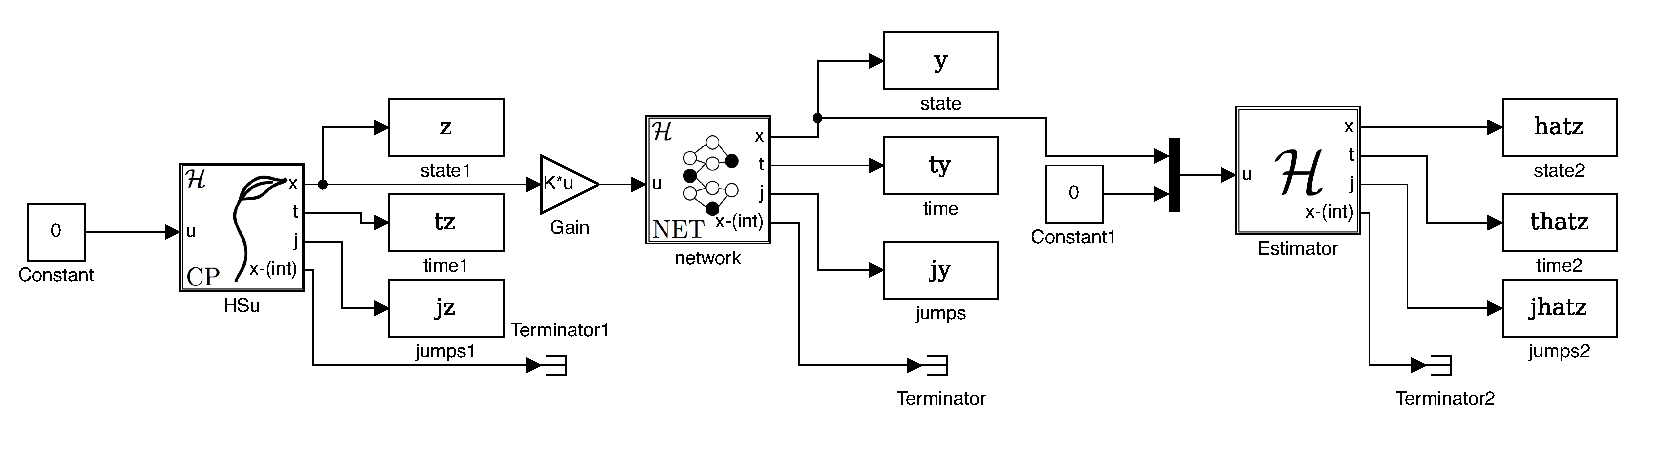
\includegraphics[width=1.0\textwidth]{figures/Simulink/NetworkExample.eps}}
   \caption{Estimation over a network scheme in Example~\ref{ex:Estimation}.}
\label{fig:NetworkExample}
  \end{center}
\end{figure}

\begin{example}{Estimation Over a Network}\label{ex:Estimation}
Consider a physical process given in terms of the state-space model
\begin{equation}
\begin{aligned}
\label{eqn:PlantForEstimation}
&\xpdot=A \xp ,\qquad 
&\yp= M \xp, \qquad & \xp \in \reals^{n_P}, \yp \in \reals^{r_P}
\end{aligned}
\end{equation}
where $\xp$ is the state and $y$ is the measured output.
The output is digitally transmitted through a network.
At the other end of the network, a computer receives the information
and runs an algorithm that takes the measurements of 
$\yp$ to estimate the state $\xp$ of the physical process.
In Figure~\ref{fig:NetworkExample} the scheme of the simulation is presented.
We consider an estimation algorithm with a state variable $\hat\xp \in \reals^{n_P}$,
which denotes the estimate of $\xp$, that is appropriately reset
to a new value involving the information received.
More precisely, denoting the transmission times by $t_i$
and $L$ a constant matrix to be designed,
the estimation algorithm updates its state as follows
\begin{equation}\label{eqn:HatXpUpdateExample}
\hat\xp^+=\hat\xp+L(\yp-M\hat\xp)
\end{equation}
at every instant information is received.
In between such events, the algorithm
updates its state continuously so as to match the evolution
of the state of the physical process, that is, via
\begin{equation}\label{eqn:HatXpFlowsExample}
\dot{\hat\xp} = A \hat\xp
\end{equation}
Modeling the network as a hybrid system,
which, in particular, assumes zero transmission delay,
the state variables of the entire system are 
$j_N$, $\tau_N \in \reals$, $m_N \in \reals^{r_P}$, and $\xp,\ \hat\xp\in \reals^{n_P}$.  
Then, transmissions occur when $\tau_N \leq 0$, 
at which events the state of the network is updated via
$$
\tau_N^+ \in [T^{*\min}_{N},T^{*\max}_{N}],\quad j_N^+ = j_N+1, \qquad m_N^+ = \yp
$$
and the state of the algorithm is updated via \eqref{eqn:HatXpUpdateExample}.
Note that since the state of the physical process does not change at such
events, we can use the following trivial difference equation to update it at the
network events:
$$
\xp^+ = \xp
$$
In between events, the state of the network is updated as
$$
\dot{\tau}_N = -1, \qquad \dot{j}_N, \qquad \dot{m}_N = 0
$$
the state of the algorithm changes continuously according to \eqref{eqn:HatXpFlowsExample}, and the 
state of the physical process changes according to \eqref{eqn:PlantForEstimation}.
Considering the equations above, we arbitrarily pick the following data for each of the subsystems in Figure~\ref{fig:NetworkExample}:

\begin{itemize}
\item Physical process:
\begin{eqnarray}
\fp(\xp, u):= A\xp + Bu,\ 
   \Cp : = \Re^{n_p}\times\Re\\
\gp(\xp, u):= \xp,\ 
    \Dp: =\emptyset,\ 
\yp = h(\xp) : =M\xp
\end{eqnarray}
where 
\begin{align}
A = 
\begin{bmatrix} 
0&1&0&0\\
-1&0&0&0\\
-2&1&-1&0\\
2&-2&0&-2
\end{bmatrix},\quad
B = \begin{bmatrix} 0\\0\\0\\0 \end{bmatrix},\quad
M = \begin{bmatrix}1&0&0&0\end{bmatrix},
\end{align}
$n_p=4$, $r_p=1$, $\xp \in\Re^{n_p}$, $\yp\in\Re^{r_p}$, and $u\in\Re$.

\item Network: 

\begin{align}
f(x_N, u_N)&:= \begin{bmatrix}
0\\0\\-1
\end{bmatrix},\ 
   &C &:= \defset{(x_N,u_N)}{ \tau_N \geq 0 },\\
g(x_N, u_N)&:= \begin{bmatrix}
u_N\\
j_N+1\\
\tau_r
\end{bmatrix},\ 
    &D &:=\defset{(x_N,u_N)}{ \tau_N \leq 0 },\quad 
y_N = h(x_N) : =x_N
\end{align}
where 
$\tau_r\in[T^{*\min}_{N},T^{*\max}_{N}]$ is a random variable that models the time in-between communication instances. Also, the sate and the input are given by $x_N=(m_N,j_N,\tau_N)\in\Re\times\Re\times\Re$, and $u_N=\yp\in\Re^{r_p}$, respectively.
\item Estimator:
\begin{align}
f(x_E, u_E)&:= 
\begin{bmatrix}
A &0 \\ 0 & 0
\end{bmatrix}x_E + \begin{bmatrix}
B\\0
\end{bmatrix}v,\ 
   &C &:= \defset{(x_E,u_E)}{ j_E = j_N },\\ 
g((\hat{x},j_E), u_E)&:= \begin{bmatrix}
\hat{x} + L(m_N-M\hat{x})\\
j_N
\end{bmatrix},\ 
    &D &:=\defset{(x,u)}{ j_E\in\nats\setminus j_N},
\end{align}
where $L$, which is designed as in~\cite{FGST16}, is given by
\begin{align}
L &:= \begin{bmatrix} 1\\ -0.9433\\ -0.6773\\1.6274\end{bmatrix},
\end{align}
the input and the state are given by $u_E = (x_N,v) = ((m_N,j_N,\tau_N),v)\in\Re\times\Re\times\Re\times\Re$, and $x_E=(\hat{x},j_E)\in\Re^{4}\times\Re$, respectively. Notice that the estimator block (Estimator) in Figure~\ref{fig:NetworkExample} is implemented using a regular hybrid system block with embedded functions.

\end{itemize}

%\begin{eqnarray}
%f(x, u):= ,\ 
%   C : = \defset{(x,u)}{ },\\
%g(x, u):= ,\ 
%    D: =\defset{(x,u)}{ },\ 
%y = h(x) : =x
%\end{eqnarray}


For each hybrid system in Figure~\ref{fig:NetworkExample} (HSu, network, and Estimator) we have the following Matlab embedded functions that describe the sets $C$ and $D$ and functions $f$ and $g$.
Figure~\ref{fig:Net-Est} depicts the corresponding hybrid arc for the position state.

\begin{figure}[ht]
  \begin{center}
    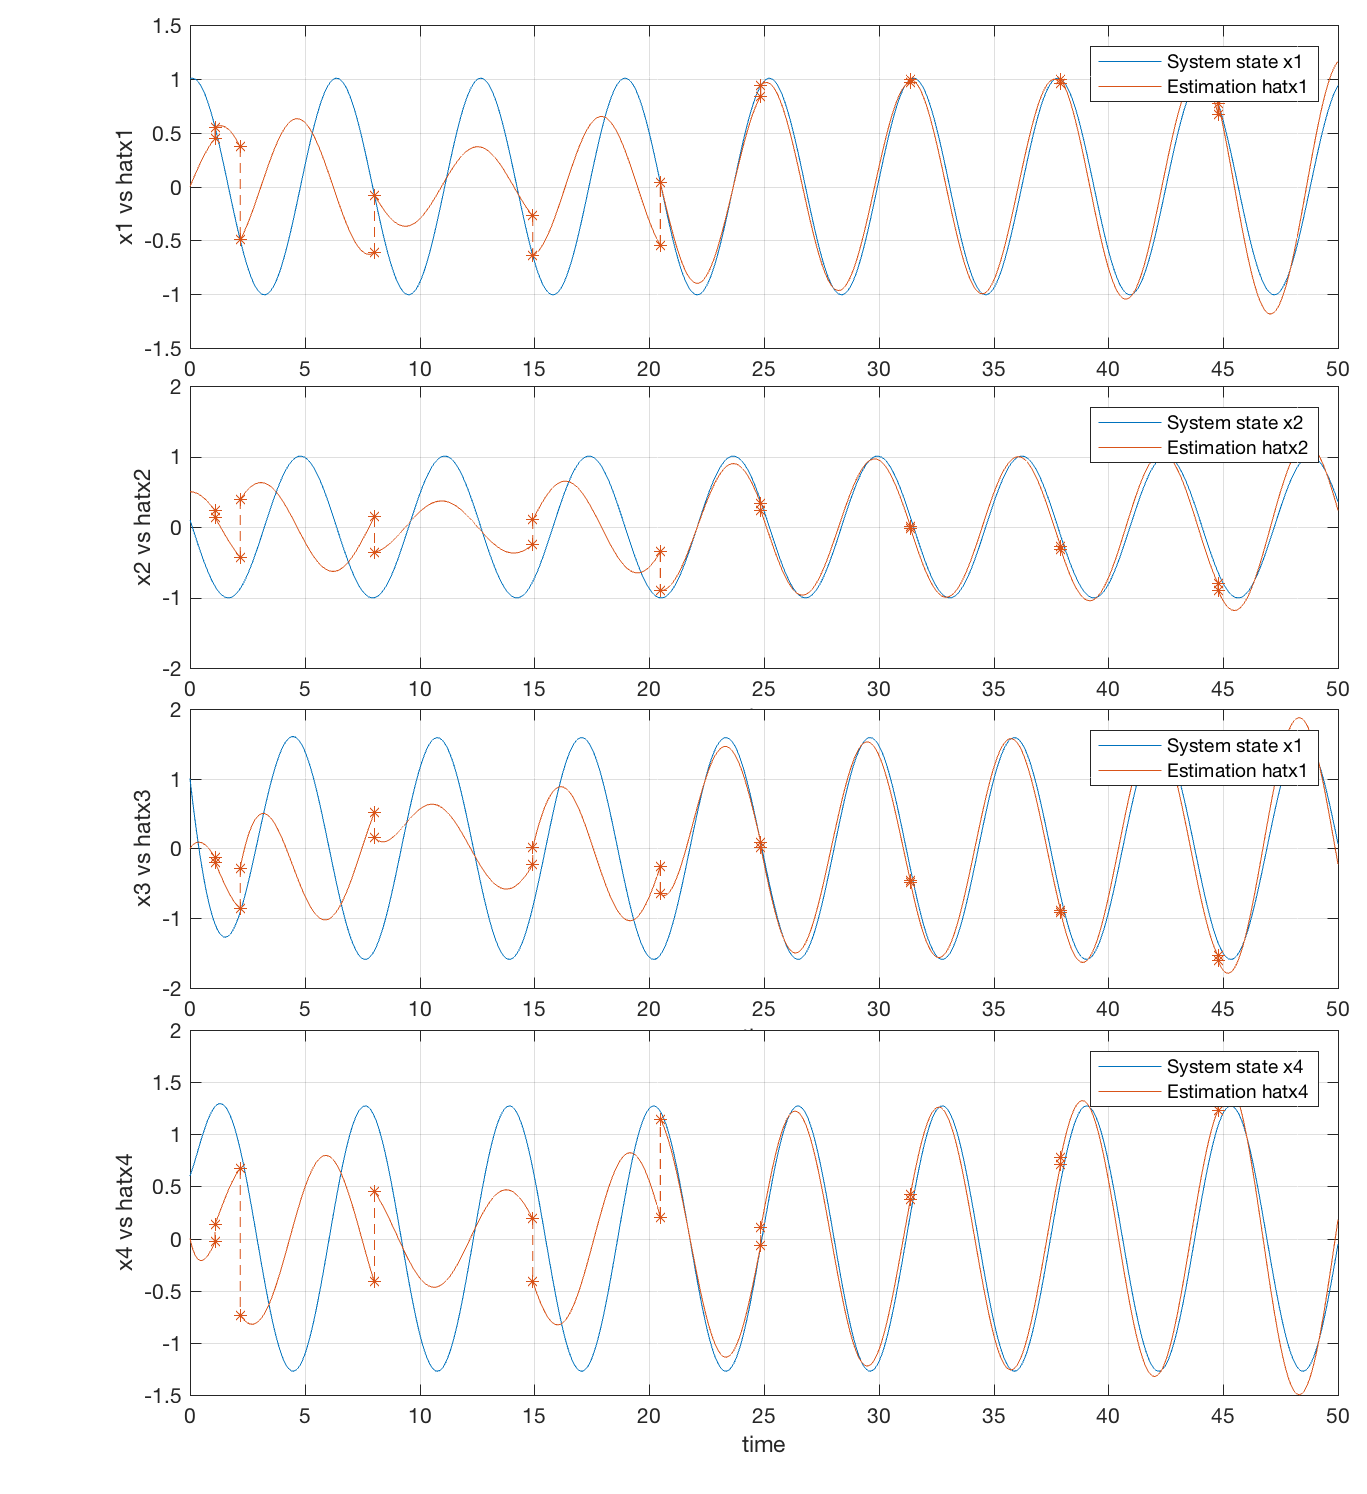
\includegraphics[width=0.8\textwidth]{figures/Simulink/ResultsNetworkEstimator1.eps}
   \caption{Estimated states Vs. continuous plant states}
\label{fig:Net-Est}
  \end{center}
\end{figure}

% Set the location for MATLAB files included via the "\code" command.
\codeLocation{Matlab2tex_CPS_Network_1}

\begin{itemize}
\item Continuous process:

\code{f.m}
\code{C.m}
\code{g.m}
\code{D.m}

% Flow map
% %\scriptsize
% % This file was automatically created from the m-file 
% "m2tex.m" written by USL. 
% The fontencoding in this file is UTF-8. 
%  
% You will need to include the following two packages in 
% your LaTeX-Main-File. 
%  
% \usepackage{color} 
% \usepackage{fancyvrb} 
%  
% It is advised to use the following option for Inputenc 
% \usepackage[utf8]{inputenc} 
%  
  
% definition of matlab colors: 
\definecolor{mblue}{rgb}{0,0,1} 
\definecolor{mgreen}{rgb}{0.13333,0.5451,0.13333} 
\definecolor{mred}{rgb}{0.62745,0.12549,0.94118} 
\definecolor{mgrey}{rgb}{0.5,0.5,0.5} 
\definecolor{mdarkgrey}{rgb}{0.25,0.25,0.25} 
  
\DefineShortVerb[fontfamily=courier,fontseries=m]{\$} 
\DefineShortVerb[fontfamily=courier,fontseries=b]{\#} 
  
\noindent                    
 \hspace*{-1.6em}{\scriptsize 1}$  $\color{mblue}$function$\color{black}$ xdot = f(x, u, gamma)$\\
 \hspace*{-1.6em}{\scriptsize 2}$  $\\
 \hspace*{-1.6em}{\scriptsize 3}$  $\color{mgreen}#%%%%%%%%%%%%%%%%%%%%%%%%%%%%%%%%%%%%%%%%%%%%%%%%%%%%%%%%%%%%%%%%%%%%%%%%%%%#\color{black}$$\\
 \hspace*{-1.6em}{\scriptsize 4}$  $\color{mgreen}$% Matlab Function  Author: Ricardo Sanfelice $\color{black}$$\\
 \hspace*{-1.6em}{\scriptsize 5}$  $\color{mgreen}$% (Revised by Giampiero Campa)$\color{black}$$\\
 \hspace*{-1.6em}{\scriptsize 6}$  $\color{mgreen}$% (Revised by Pablo Nanez)$\color{black}$$\\
 \hspace*{-1.6em}{\scriptsize 7}$  $\color{mgreen}$%$\color{black}$$\\
 \hspace*{-1.6em}{\scriptsize 8}$  $\color{mgreen}$% Project: Simulation of a hybrid system (Bouncing Ball)$\color{black}$$\\
 \hspace*{-1.6em}{\scriptsize 9}$  $\color{mgreen}$%$\color{black}$$\\
 \hspace*{-2em}{\scriptsize 10}$  $\color{mgreen}$% Name: f.m$\color{black}$$\\
 \hspace*{-2em}{\scriptsize 11}$  $\color{mgreen}$%$\color{black}$$\\
 \hspace*{-2em}{\scriptsize 12}$  $\color{mgreen}$% Description: Flow map$\color{black}$$\\
 \hspace*{-2em}{\scriptsize 13}$  $\color{mgreen}$%$\color{black}$$\\
 \hspace*{-2em}{\scriptsize 14}$  $\color{mgreen}$% Version: 1.0$\color{black}$$\\
 \hspace*{-2em}{\scriptsize 15}$  $\color{mgreen}$% Required files: - $\color{black}$$\\
 \hspace*{-2em}{\scriptsize 16}$  $\color{mgreen}#%%%%%%%%%%%%%%%%%%%%%%%%%%%%%%%%%%%%%%%%%%%%%%%%%%%%%%%%%%%%%%%%%%%%%%%%%%%#\color{black}$$\\
 \hspace*{-2em}{\scriptsize 17}$  $\\
 \hspace*{-2em}{\scriptsize 18}$  $\\
 \hspace*{-2em}{\scriptsize 19}$  $\color{mgreen}$% flow map: xdot=f(x,u);$\color{black}$$\\
 \hspace*{-2em}{\scriptsize 20}$  xdot = [x(2); gamma];$\\ 
  
\UndefineShortVerb{\$} 
\UndefineShortVerb{\#}\label{scr:f}
% %\normalsize

% Flow set
% %\scriptsize
% % This file was automatically created from the m-file 
% "m2tex.m" written by USL. 
% The fontencoding in this file is UTF-8. 
%  
% You will need to include the following two packages in 
% your LaTeX-Main-File. 
%  
% \usepackage{color} 
% \usepackage{fancyvrb} 
%  
% It is advised to use the following option for Inputenc 
% \usepackage[utf8]{inputenc} 
%  
  
% definition of matlab colors: 
\definecolor{mblue}{rgb}{0,0,1} 
\definecolor{mgreen}{rgb}{0.13333,0.5451,0.13333} 
\definecolor{mred}{rgb}{0.62745,0.12549,0.94118} 
\definecolor{mgrey}{rgb}{0.5,0.5,0.5} 
\definecolor{mdarkgrey}{rgb}{0.25,0.25,0.25} 
  
\DefineShortVerb[fontfamily=courier,fontseries=m]{\$} 
\DefineShortVerb[fontfamily=courier,fontseries=b]{\#} 
  
\noindent                          
 \hspace*{-1.6em}{\scriptsize 1}$  $\color{mblue}$function$\color{black}$ v  = C(x, u)$\\
 \hspace*{-1.6em}{\scriptsize 2}$  $\color{mgreen}$%--------------------------------------------------------------------------$\color{black}$$\\
 \hspace*{-1.6em}{\scriptsize 3}$  $\color{mgreen}$% Matlab M-file Project: HyEQ Toolbox @  Hybrid Systems Laboratory (HSL),$\color{black}$$\\
 \hspace*{-1.6em}{\scriptsize 4}$  $\color{mgreen}$% https://hybrid.soe.ucsc.edu/software$\color{black}$$\\
 \hspace*{-1.6em}{\scriptsize 5}$  $\color{mgreen}$% http://hybridsimulator.wordpress.com/$\color{black}$$\\
 \hspace*{-1.6em}{\scriptsize 6}$  $\color{mgreen}$%--------------------------------------------------------------------------$\color{black}$$\\
 \hspace*{-1.6em}{\scriptsize 7}$  $\color{mgreen}$% Project: Simulation of a hybrid system$\color{black}$$\\
 \hspace*{-1.6em}{\scriptsize 8}$  $\color{mgreen}$% Description: Flow set$\color{black}$$\\
 \hspace*{-1.6em}{\scriptsize 9}$  $\color{mgreen}$%--------------------------------------------------------------------------$\color{black}$$\\
 \hspace*{-2em}{\scriptsize 10}$  $\color{mgreen}$%--------------------------------------------------------------------------$\color{black}$$\\
 \hspace*{-2em}{\scriptsize 11}$  $\color{mgreen}$%   See also HYEQSOLVER, PLOTARC, PLOTARC3, PLOTFLOWS, PLOTHARC,$\color{black}$$\\
 \hspace*{-2em}{\scriptsize 12}$  $\color{mgreen}$%   PLOTHARCCOLOR, PLOTHARCCOLOR3D, PLOTHYBRIDARC, PLOTJUMPS.$\color{black}$$\\
 \hspace*{-2em}{\scriptsize 13}$  $\color{mgreen}$%   Copyright @ Hybrid Systems Laboratory (HSL),$\color{black}$$\\
 \hspace*{-2em}{\scriptsize 14}$  $\color{mgreen}$%   Revision: 0.0.0.3 Date: 05/20/2015 3:42:00$\color{black}$$\\
 \hspace*{-2em}{\scriptsize 15}$  $\color{mgreen}$%$\color{black}$$\\
 \hspace*{-2em}{\scriptsize 16}$  $\color{mgreen}$% Check on flow conditions$\color{black}$$\\
 \hspace*{-2em}{\scriptsize 17}$  $\color{mgreen}$% E.g.,$\color{black}$$\\
 \hspace*{-2em}{\scriptsize 18}$  $\color{mgreen}$% if (x(1) >= u(1))  % flow condition$\color{black}$$\\
 \hspace*{-2em}{\scriptsize 19}$  $\color{mgreen}$%     v = 1;  % report flow$\color{black}$$\\
 \hspace*{-2em}{\scriptsize 20}$  $\color{mgreen}$% else$\color{black}$$\\
 \hspace*{-2em}{\scriptsize 21}$  $\color{mgreen}$%     v = 0;   % do not report flow$\color{black}$$\\
 \hspace*{-2em}{\scriptsize 22}$  $\color{mgreen}$% end$\color{black}$$\\
 \hspace*{-2em}{\scriptsize 23}$  $\\
 \hspace*{-2em}{\scriptsize 24}$  $\\
 \hspace*{-2em}{\scriptsize 25}$  v = 1; $\color{mgreen}$% report flow$\color{black}$$\\
 \hspace*{-2em}{\scriptsize 26}$  $\\ 
  
\UndefineShortVerb{\$} 
\UndefineShortVerb{\#}\label{scr:C}
% %\normalsize

% Jump map
% %\scriptsize
% % This file was automatically created from the m-file 
% "m2tex.m" written by USL. 
% The fontencoding in this file is UTF-8. 
%  
% You will need to include the following two packages in 
% your LaTeX-Main-File. 
%  
% \usepackage{color} 
% \usepackage{fancyvrb} 
%  
% It is advised to use the following option for Inputenc 
% \usepackage[utf8]{inputenc} 
%  
  
% definition of matlab colors: 
\definecolor{mblue}{rgb}{0,0,1} 
\definecolor{mgreen}{rgb}{0.13333,0.5451,0.13333} 
\definecolor{mred}{rgb}{0.62745,0.12549,0.94118} 
\definecolor{mgrey}{rgb}{0.5,0.5,0.5} 
\definecolor{mdarkgrey}{rgb}{0.25,0.25,0.25} 
  
\DefineShortVerb[fontfamily=courier,fontseries=m]{\$} 
\DefineShortVerb[fontfamily=courier,fontseries=b]{\#} 
  
\noindent   
 \hspace*{-1.6em}{\scriptsize 1}$  $\color{mblue}$function$\color{black}$ xplus = g(x, u, lambda)$\\
 \hspace*{-1.6em}{\scriptsize 2}$  $\color{mgreen}$% jump map$\color{black}$$\\
 \hspace*{-1.6em}{\scriptsize 3}$  xplus = [u(1); -lambda*x(2)];$\\ 
  
\UndefineShortVerb{\$} 
\UndefineShortVerb{\#}\label{scr:g}
% %\normalsize

% Jump set
% %\scriptsize
% % This file was automatically created from the m-file 
% "m2tex.m" written by USL. 
% The fontencoding in this file is UTF-8. 
%  
% You will need to include the following two packages in 
% your LaTeX-Main-File. 
%  
% \usepackage{color} 
% \usepackage{fancyvrb} 
%  
% It is advised to use the following option for Inputenc 
% \usepackage[utf8]{inputenc} 
%  
  
% definition of matlab colors: 
\definecolor{mblue}{rgb}{0,0,1} 
\definecolor{mgreen}{rgb}{0.13333,0.5451,0.13333} 
\definecolor{mred}{rgb}{0.62745,0.12549,0.94118} 
\definecolor{mgrey}{rgb}{0.5,0.5,0.5} 
\definecolor{mdarkgrey}{rgb}{0.25,0.25,0.25} 
  
\DefineShortVerb[fontfamily=courier,fontseries=m]{\$} 
\DefineShortVerb[fontfamily=courier,fontseries=b]{\#} 
  
\noindent                         
 \hspace*{-1.6em}{\scriptsize 1}$  $\color{mblue}$function$\color{black}$ v  = D(x, u) $\\
 \hspace*{-1.6em}{\scriptsize 2}$  $\\
 \hspace*{-1.6em}{\scriptsize 3}$  $\color{mgreen}#%%%%%%%%%%%%%%%%%%%%%%%%%%%%%%%%%%%%%%%%%%%%%%%%%%%%%%%%%%%%%%%%%%%%%%%%%%%#\color{black}$$\\
 \hspace*{-1.6em}{\scriptsize 4}$  $\color{mgreen}$% Matlab Function  Author: Ricardo Sanfelice $\color{black}$$\\
 \hspace*{-1.6em}{\scriptsize 5}$  $\color{mgreen}$% (Revised by Giampiero Campa)$\color{black}$$\\
 \hspace*{-1.6em}{\scriptsize 6}$  $\color{mgreen}$% (Revised by Pablo Nanez)$\color{black}$$\\
 \hspace*{-1.6em}{\scriptsize 7}$  $\color{mgreen}$%$\color{black}$$\\
 \hspace*{-1.6em}{\scriptsize 8}$  $\color{mgreen}$% Project: Simulation of a hybrid system (Bouncing ball)$\color{black}$$\\
 \hspace*{-1.6em}{\scriptsize 9}$  $\color{mgreen}$%$\color{black}$$\\
 \hspace*{-2em}{\scriptsize 10}$  $\color{mgreen}$% Name: D.m$\color{black}$$\\
 \hspace*{-2em}{\scriptsize 11}$  $\color{mgreen}$%$\color{black}$$\\
 \hspace*{-2em}{\scriptsize 12}$  $\color{mgreen}$% Description: Jump set$\color{black}$$\\
 \hspace*{-2em}{\scriptsize 13}$  $\color{mgreen}$%$\color{black}$$\\
 \hspace*{-2em}{\scriptsize 14}$  $\color{mgreen}$% Version: 1.0$\color{black}$$\\
 \hspace*{-2em}{\scriptsize 15}$  $\color{mgreen}$% Required files: - $\color{black}$$\\
 \hspace*{-2em}{\scriptsize 16}$  $\color{mgreen}#%%%%%%%%%%%%%%%%%%%%%%%%%%%%%%%%%%%%%%%%%%%%%%%%%%%%%%%%%%%%%%%%%%%%%%%%%%%#\color{black}$$\\
 \hspace*{-2em}{\scriptsize 17}$  $\\
 \hspace*{-2em}{\scriptsize 18}$  xtemp = zeros(2,1);$\\
 \hspace*{-2em}{\scriptsize 19}$  xtemp = x;$\\
 \hspace*{-2em}{\scriptsize 20}$  $\\
 \hspace*{-2em}{\scriptsize 21}$  $\color{mblue}$if$\color{black}$ (xtemp(1) <= u(1)) && (xtemp(2) <= 0)  $\color{mgreen}$% jump condition$\color{black}$$\\
 \hspace*{-2em}{\scriptsize 22}$      v = 1;  $\color{mgreen}$% report jump$\color{black}$$\\
 \hspace*{-2em}{\scriptsize 23}$  $\color{mblue}$else$\color{black}$$\\
 \hspace*{-2em}{\scriptsize 24}$      v = 0;   $\color{mgreen}$% do not report jump$\color{black}$$\\
 \hspace*{-2em}{\scriptsize 25}$  $\color{mblue}$end$\color{black}$$\\ 
  
\UndefineShortVerb{\$} 
\UndefineShortVerb{\#}\label{scr:D}
% %\normalsize

\item Network:

\code{f\_network.m}
\code{C\_network.m}
\code{g\_network.m}
\code{D\_network.m}

% Flow map
% %\scriptsize
% % This file was automatically created from the m-file 
% "m2tex.m" written by USL. 
% The fontencoding in this file is UTF-8. 
%  
% You will need to include the following two packages in 
% your LaTeX-Main-File. 
%  
% \usepackage{color} 
% \usepackage{fancyvrb} 
%  
% It is advised to use the following option for Inputenc 
% \usepackage[utf8]{inputenc} 
%  
  
% definition of matlab colors: 
\definecolor{mblue}{rgb}{0,0,1} 
\definecolor{mgreen}{rgb}{0.13333,0.5451,0.13333} 
\definecolor{mred}{rgb}{0.62745,0.12549,0.94118} 
\definecolor{mgrey}{rgb}{0.5,0.5,0.5} 
\definecolor{mdarkgrey}{rgb}{0.25,0.25,0.25} 
  
\DefineShortVerb[fontfamily=courier,fontseries=m]{\$} 
\DefineShortVerb[fontfamily=courier,fontseries=b]{\#} 
  
\begin{Verbatim}[commandchars=\$\{\},numbers=left,numbersep=2pt] 

    $textcolor{mblue}{function} xdot = f(x,vs) 
    $textcolor{mgreen}{%--------------------------------------------------------------------------} 
    $textcolor{mgreen}{% Matlab M-file Project: HyEQ Toolbox @  Hybrid Systems Laboratory (HSL), } 
    $textcolor{mgreen}{% https://hybrid.soe.ucsc.edu/software} 
    $textcolor{mgreen}{% http://hybridsimulator.wordpress.com/} 
    $textcolor{mgreen}{%--------------------------------------------------------------------------} 
    $textcolor{mgreen}{% Project: Simulation of a hybrid system Digital network (net) } 
    $textcolor{mgreen}{% Description: Flow map} 
    $textcolor{mgreen}{%--------------------------------------------------------------------------} 
    $textcolor{mgreen}{%--------------------------------------------------------------------------} 
    $textcolor{mgreen}{%   See also HYEQSOLVER, PLOTARC, PLOTARC3, PLOTFLOWS, PLOTHARC,} 
    $textcolor{mgreen}{%   PLOTHARCCOLOR, PLOTHARCCOLOR3D, PLOTHYBRIDARC, PLOTJUMPS.} 
    $textcolor{mgreen}{%   Copyright @ Hybrid Systems Laboratory (HSL),} 
    $textcolor{mgreen}{%   Revision: 0.0.0.3 Date: 05/20/2015 3:42:00} 
     
    n = length(vs); $textcolor{mgreen}{% measured input size} 
     
    msdot = zeros(n,1); $textcolor{mgreen}{% measured continuous dynamics} 
    jdot = 0; 
    tau_sdot = -1; $textcolor{mgreen}{% Timer tau_s} 
    xdot = [msdot;jdot;tau_sdot]; 
      
\end{Verbatim}  
  
\UndefineShortVerb{\$} 
\UndefineShortVerb{\#} 
 \label{scr:f}
% %\normalsize

% Flow set
% %\scriptsize
% % This file was automatically created from the m-file 
% "m2tex.m" written by USL. 
% The fontencoding in this file is UTF-8. 
%  
% You will need to include the following two packages in 
% your LaTeX-Main-File. 
%  
% \usepackage{color} 
% \usepackage{fancyvrb} 
%  
% It is advised to use the following option for Inputenc 
% \usepackage[utf8]{inputenc} 
%  
  
% definition of matlab colors: 
\definecolor{mblue}{rgb}{0,0,1} 
\definecolor{mgreen}{rgb}{0.13333,0.5451,0.13333} 
\definecolor{mred}{rgb}{0.62745,0.12549,0.94118} 
\definecolor{mgrey}{rgb}{0.5,0.5,0.5} 
\definecolor{mdarkgrey}{rgb}{0.25,0.25,0.25} 
  
\DefineShortVerb[fontfamily=courier,fontseries=m]{\$} 
\DefineShortVerb[fontfamily=courier,fontseries=b]{\#} 
  
\begin{Verbatim}[commandchars=\$\{\},numbers=left,numbersep=2pt] 

    $textcolor{mblue}{function} v  = C(x, vs, Tnmax)  
    $textcolor{mgreen}{%--------------------------------------------------------------------------} 
    $textcolor{mgreen}{% Matlab M-file Project: HyEQ Toolbox @  Hybrid Systems Laboratory (HSL), } 
    $textcolor{mgreen}{% https://hybrid.soe.ucsc.edu/software} 
    $textcolor{mgreen}{% http://hybridsimulator.wordpress.com/} 
    $textcolor{mgreen}{%--------------------------------------------------------------------------} 
    $textcolor{mgreen}{% Project: Simulation of a hybrid system Digital network (net) } 
    $textcolor{mgreen}{% Description: Flow set} 
    $textcolor{mgreen}{%--------------------------------------------------------------------------} 
    $textcolor{mgreen}{%--------------------------------------------------------------------------} 
    $textcolor{mgreen}{%   See also HYEQSOLVER, PLOTARC, PLOTARC3, PLOTFLOWS, PLOTHARC,} 
    $textcolor{mgreen}{%   PLOTHARCCOLOR, PLOTHARCCOLOR3D, PLOTHYBRIDARC, PLOTJUMPS.} 
    $textcolor{mgreen}{%   Copyright @ Hybrid Systems Laboratory (HSL),} 
    $textcolor{mgreen} 
    $textcolor{mgreen}{% Check on flow conditions} 
    $textcolor{mgreen}{% E.g.,} 
    $textcolor{mgreen}{% if (x(1) >= u(1))  % flow condition} 
    $textcolor{mgreen}{%     v = 1;  % report flow} 
    $textcolor{mgreen}{% else} 
    $textcolor{mgreen}{%     v = 0;   % do not report flow} 
    $textcolor{mgreen}{% end} 
     
    tau_s = x(end); $textcolor{mgreen}{% timer state} 
     
    $textcolor{mblue}{if} tau_s>=0 && tau_s<= Tnmax 
        v = 1; $textcolor{mgreen}{% report flow} 
    $textcolor{mblue}{elseif} tau_s> Tnmax 
        v = 0; $textcolor{mgreen}{% do not report flow} 
    $textcolor{mblue}{else} 
        v = 0; 
    $textcolor{mblue}{end}  
\end{Verbatim}  
  
\UndefineShortVerb{\$} 
\UndefineShortVerb{\#} 
 \label{scr:C}
% %\normalsize

% Jump map
% %\scriptsize
% % This file was automatically created from the m-file 
% "m2tex.m" written by USL. 
% The fontencoding in this file is UTF-8. 
%  
% You will need to include the following two packages in 
% your LaTeX-Main-File. 
%  
% \usepackage{color} 
% \usepackage{fancyvrb} 
%  
% It is advised to use the following option for Inputenc 
% \usepackage[utf8]{inputenc} 
%  
  
% definition of matlab colors: 
\definecolor{mblue}{rgb}{0,0,1} 
\definecolor{mgreen}{rgb}{0.13333,0.5451,0.13333} 
\definecolor{mred}{rgb}{0.62745,0.12549,0.94118} 
\definecolor{mgrey}{rgb}{0.5,0.5,0.5} 
\definecolor{mdarkgrey}{rgb}{0.25,0.25,0.25} 
  
\DefineShortVerb[fontfamily=courier,fontseries=m]{\$} 
\DefineShortVerb[fontfamily=courier,fontseries=b]{\#} 
  
\noindent                              
 \hspace*{-1.6em}{\scriptsize 1}$  $\color{mblue}$function$\color{black}$ xplus = g(x, vs, Tnmax, Tnmin, tk)$\\
 \hspace*{-1.6em}{\scriptsize 2}$  $\color{mgreen}$%--------------------------------------------------------------------------$\color{black}$$\\
 \hspace*{-1.6em}{\scriptsize 3}$  $\color{mgreen}$% Matlab M-file Project: HyEQ Toolbox @  Hybrid Systems Laboratory (HSL), $\color{black}$$\\
 \hspace*{-1.6em}{\scriptsize 4}$  $\color{mgreen}$% https://hybrid.soe.ucsc.edu/software$\color{black}$$\\
 \hspace*{-1.6em}{\scriptsize 5}$  $\color{mgreen}$% http://hybridsimulator.wordpress.com/$\color{black}$$\\
 \hspace*{-1.6em}{\scriptsize 6}$  $\color{mgreen}$%--------------------------------------------------------------------------$\color{black}$$\\
 \hspace*{-1.6em}{\scriptsize 7}$  $\color{mgreen}$% Project: Simulation of a hybrid system Analog-to-Digital converter (ADC) $\color{black}$$\\
 \hspace*{-1.6em}{\scriptsize 8}$  $\color{mgreen}$% Description: Jump map$\color{black}$$\\
 \hspace*{-1.6em}{\scriptsize 9}$  $\color{mgreen}$%--------------------------------------------------------------------------$\color{black}$$\\
 \hspace*{-2em}{\scriptsize 10}$  $\color{mgreen}$%--------------------------------------------------------------------------$\color{black}$$\\
 \hspace*{-2em}{\scriptsize 11}$  $\color{mgreen}$%   See also HYEQSOLVER, PLOTARC, PLOTARC3, PLOTFLOWS, PLOTHARC,$\color{black}$$\\
 \hspace*{-2em}{\scriptsize 12}$  $\color{mgreen}$%   PLOTHARCCOLOR, PLOTHARCCOLOR3D, PLOTHYBRIDARC, PLOTJUMPS.$\color{black}$$\\
 \hspace*{-2em}{\scriptsize 13}$  $\color{mgreen}$%   Copyright @ Hybrid Systems Laboratory (HSL),$\color{black}$$\\
 \hspace*{-2em}{\scriptsize 14}$  $\color{mgreen}$%   Revision: 0.0.0.3 Date: 05/20/2015 3:42:00$\color{black}$$\\
 \hspace*{-2em}{\scriptsize 15}$  $\\
 \hspace*{-2em}{\scriptsize 16}$  n = length(vs); $\color{mgreen}$% measured input size$\color{black}$$\\
 \hspace*{-2em}{\scriptsize 17}$  xtemp = zeros(n+2,1);$\\
 \hspace*{-2em}{\scriptsize 18}$  xtemp = x;$\\
 \hspace*{-2em}{\scriptsize 19}$  x = xtemp;$\\
 \hspace*{-2em}{\scriptsize 20}$  $\\
 \hspace*{-2em}{\scriptsize 21}$  $\\
 \hspace*{-2em}{\scriptsize 22}$  j = x(n+1);$\\
 \hspace*{-2em}{\scriptsize 23}$  msplus = vs; $\color{mgreen}$% output = measured input$\color{black}$$\\
 \hspace*{-2em}{\scriptsize 24}$  $\color{mgreen}$% The value tau_s is updated as a function of vs, e.g., $\color{black}$$\\
 \hspace*{-2em}{\scriptsize 25}$  tau_splus = tk(j+1); $\color{mgreen}$% Timer tau_s$\color{black}$$\\
 \hspace*{-2em}{\scriptsize 26}$  j_plus = j+1;$\\
 \hspace*{-2em}{\scriptsize 27}$  xplus = [msplus;j_plus;tau_splus];$\\
 \hspace*{-2em}{\scriptsize 28}$  $\\
 \hspace*{-2em}{\scriptsize 29}$  $\\
 \hspace*{-2em}{\scriptsize 30}$  $\\ 
  
\UndefineShortVerb{\$} 
\UndefineShortVerb{\#}\label{scr:g}
% %\normalsize

% Jump set
% %\scriptsize
% % This file was automatically created from the m-file 
% "m2tex.m" written by USL. 
% The fontencoding in this file is UTF-8. 
%  
% You will need to include the following two packages in 
% your LaTeX-Main-File. 
%  
% \usepackage{color} 
% \usepackage{fancyvrb} 
%  
% It is advised to use the following option for Inputenc 
% \usepackage[utf8]{inputenc} 
%  
  
% definition of matlab colors: 
\definecolor{mblue}{rgb}{0,0,1} 
\definecolor{mgreen}{rgb}{0.13333,0.5451,0.13333} 
\definecolor{mred}{rgb}{0.62745,0.12549,0.94118} 
\definecolor{mgrey}{rgb}{0.5,0.5,0.5} 
\definecolor{mdarkgrey}{rgb}{0.25,0.25,0.25} 
  
\DefineShortVerb[fontfamily=courier,fontseries=m]{\$} 
\DefineShortVerb[fontfamily=courier,fontseries=b]{\#} 
  
\begin{Verbatim}[commandchars=\$\{\},numbers=left,numbersep=2pt] 

    $textcolor{mblue}{function} v  = D(x, vs)  
    $textcolor{mgreen}{%--------------------------------------------------------------------------} 
    $textcolor{mgreen}{% Matlab M-file Project: HyEQ Toolbox @  Hybrid Systems Laboratory (HSL), } 
    $textcolor{mgreen}{% https://hybrid.soe.ucsc.edu/software} 
    $textcolor{mgreen}{% http://hybridsimulator.wordpress.com/} 
    $textcolor{mgreen}{%--------------------------------------------------------------------------} 
    $textcolor{mgreen}{% Project: Simulation of a hybrid system Analog-to-Digital converter (ADC) } 
    $textcolor{mgreen}{% Description: Jump set} 
    $textcolor{mgreen}{%--------------------------------------------------------------------------} 
    $textcolor{mgreen}{%--------------------------------------------------------------------------} 
    $textcolor{mgreen}{%   See also HYEQSOLVER, PLOTARC, PLOTARC3, PLOTFLOWS, PLOTHARC,} 
    $textcolor{mgreen}{%   PLOTHARCCOLOR, PLOTHARCCOLOR3D, PLOTHYBRIDARC, PLOTJUMPS.} 
    $textcolor{mgreen}{%   Copyright @ Hybrid Systems Laboratory (HSL),} 
    $textcolor{mgreen} 
    $textcolor{mgreen}{% Check on jump conditions} 
    $textcolor{mgreen}{% % E.g.,} 
    $textcolor{mgreen}{% if (x(1) <= u(1)) && (x(2) <= 0)  % jump condition} 
    $textcolor{mgreen}{%     v = 1;  % report jump} 
    $textcolor{mgreen}{% else} 
    $textcolor{mgreen}{%     v = 0;   % do not report jump} 
    $textcolor{mgreen}{% end} 
     
     
    tau_s = x(end); $textcolor{mgreen}{% timer state} 
     
    $textcolor{mblue}{if} tau_s>=0 
        v = 0; $textcolor{mgreen}{% do not report jump} 
    $textcolor{mblue}{elseif} tau_s<= 0 
        v = 1; $textcolor{mgreen}{% report jump} 
    $textcolor{mblue}{else} 
        v = 0; 
    $textcolor{mblue}{end}  
\end{Verbatim}  
  
\UndefineShortVerb{\$} 
\UndefineShortVerb{\#} 
 \label{scr:D}
% %\normalsize

\item Estimator:

% \code{f\_Estimator.m}
{\color{red} NOTE: "f\_Estimator.m" and "g\_Estimator.m" do not exist, for some reason.}
\code{C\_Estimator.m}
% \code{g\_Estimator.m}
\code{D\_Estimator.m}

% Flow map
% %\scriptsize
% % This file was automatically created from the m-file 
% "m2tex.m" written by USL. 
% The fontencoding in this file is UTF-8. 
%  
% You will need to include the following two packages in 
% your LaTeX-Main-File. 
%  
% \usepackage{color} 
% \usepackage{fancyvrb} 
%  
% It is advised to use the following option for Inputenc 
% \usepackage[utf8]{inputenc} 
%  
  
% definition of matlab colors: 
\definecolor{mblue}{rgb}{0,0,1} 
\definecolor{mgreen}{rgb}{0.13333,0.5451,0.13333} 
\definecolor{mred}{rgb}{0.62745,0.12549,0.94118} 
\definecolor{mgrey}{rgb}{0.5,0.5,0.5} 
\definecolor{mdarkgrey}{rgb}{0.25,0.25,0.25} 
  
\DefineShortVerb[fontfamily=courier,fontseries=m]{\$} 
\DefineShortVerb[fontfamily=courier,fontseries=b]{\#} 
  
\begin{Verbatim}[commandchars=\$\{\},numbers=left,numbersep=2pt] 

    $textcolor{mblue}{function} xdot = f(x, v,ctes) 
    $textcolor{mgreen}{%--------------------------------------------------------------------------} 
    $textcolor{mgreen}{% Matlab M-file Project: HyEQ Toolbox @  Hybrid Systems Laboratory (HSL), } 
    $textcolor{mgreen}{% https://hybrid.soe.ucsc.edu/software} 
    $textcolor{mgreen}{% http://hybridsimulator.wordpress.com/} 
    $textcolor{mgreen}{%--------------------------------------------------------------------------} 
    $textcolor{mgreen}{% Project: Simulation of a hybrid system} 
    $textcolor{mgreen}{% Description: Flow map} 
    $textcolor{mgreen}{%--------------------------------------------------------------------------} 
    $textcolor{mgreen}{%--------------------------------------------------------------------------} 
    $textcolor{mgreen}{%   See also HYEQSOLVER, PLOTARC, PLOTARC3, PLOTFLOWS, PLOTHARC,} 
    $textcolor{mgreen}{%   PLOTHARCCOLOR, PLOTHARCCOLOR3D, PLOTHYBRIDARC, PLOTJUMPS.} 
    $textcolor{mgreen}{%   Copyright @ Hybrid Systems Laboratory (HSL),} 
    $textcolor{mgreen}{%   Revision: 0.0.0.3 Date: 05/20/2015 3:42:00} 
    $textcolor{mgreen}{%--------------------------------------------------------------------------} 
    $textcolor{mgreen}{% flow map: xdot=f(x,u);} 
    $textcolor{mgreen}{% ctes = [A,B,M',L,P];} 
     
    A = ctes(:,1:4); 
    B = ctes(:,5); 
    $textcolor{mgreen}{% M = ctes(:,6)';} 
    $textcolor{mgreen}{% L = ctes(:,7);} 
    n = length(A); 
    u = v(end); 
    z = x(1:n); 
    jdot = 0; 
    zdot = A*z + B*u; 
    xdot = [zdot;jdot];  
\end{Verbatim}  
  
\UndefineShortVerb{\$} 
\UndefineShortVerb{\#} 
 \label{scr:f}
% %\normalsize

% Flow set
% %\scriptsize
% % This file was automatically created from the m-file 
% "m2tex.m" written by USL. 
% The fontencoding in this file is UTF-8. 
%  
% You will need to include the following two packages in 
% your LaTeX-Main-File. 
%  
% \usepackage{color} 
% \usepackage{fancyvrb} 
%  
% It is advised to use the following option for Inputenc 
% \usepackage[utf8]{inputenc} 
%  
  
% definition of matlab colors: 
\definecolor{mblue}{rgb}{0,0,1} 
\definecolor{mgreen}{rgb}{0.13333,0.5451,0.13333} 
\definecolor{mred}{rgb}{0.62745,0.12549,0.94118} 
\definecolor{mgrey}{rgb}{0.5,0.5,0.5} 
\definecolor{mdarkgrey}{rgb}{0.25,0.25,0.25} 
  
\DefineShortVerb[fontfamily=courier,fontseries=m]{\$} 
\DefineShortVerb[fontfamily=courier,fontseries=b]{\#} 
  
\noindent                               
 \hspace*{-1.6em}{\scriptsize 1}$  $\color{mblue}$function$\color{black}$ out  = C(x, v) $\\
 \hspace*{-1.6em}{\scriptsize 2}$  $\color{mgreen}$%--------------------------------------------------------------------------$\color{black}$$\\
 \hspace*{-1.6em}{\scriptsize 3}$  $\color{mgreen}$% Matlab M-file Project: HyEQ Toolbox @  Hybrid Systems Laboratory (HSL), $\color{black}$$\\
 \hspace*{-1.6em}{\scriptsize 4}$  $\color{mgreen}$% https://hybrid.soe.ucsc.edu/software$\color{black}$$\\
 \hspace*{-1.6em}{\scriptsize 5}$  $\color{mgreen}$% http://hybridsimulator.wordpress.com/$\color{black}$$\\
 \hspace*{-1.6em}{\scriptsize 6}$  $\color{mgreen}$%--------------------------------------------------------------------------$\color{black}$$\\
 \hspace*{-1.6em}{\scriptsize 7}$  $\color{mgreen}$% Project: Simulation of a hybrid system$\color{black}$$\\
 \hspace*{-1.6em}{\scriptsize 8}$  $\color{mgreen}$% Description: Flow set$\color{black}$$\\
 \hspace*{-1.6em}{\scriptsize 9}$  $\color{mgreen}$%--------------------------------------------------------------------------$\color{black}$$\\
 \hspace*{-2em}{\scriptsize 10}$  $\color{mgreen}$%--------------------------------------------------------------------------$\color{black}$$\\
 \hspace*{-2em}{\scriptsize 11}$  $\color{mgreen}$%   See also HYEQSOLVER, PLOTARC, PLOTARC3, PLOTFLOWS, PLOTHARC,$\color{black}$$\\
 \hspace*{-2em}{\scriptsize 12}$  $\color{mgreen}$%   PLOTHARCCOLOR, PLOTHARCCOLOR3D, PLOTHYBRIDARC, PLOTJUMPS.$\color{black}$$\\
 \hspace*{-2em}{\scriptsize 13}$  $\color{mgreen}$%   Copyright @ Hybrid Systems Laboratory (HSL),$\color{black}$$\\
 \hspace*{-2em}{\scriptsize 14}$  $\color{mgreen}$%   Revision: 0.0.0.3 Date: 05/20/2015 3:42:00$\color{black}$$\\
 \hspace*{-2em}{\scriptsize 15}$  $\color{mgreen}$%$\color{black}$$\\
 \hspace*{-2em}{\scriptsize 16}$  $\color{mgreen}$% Check on flow conditions$\color{black}$$\\
 \hspace*{-2em}{\scriptsize 17}$  $\color{mgreen}$% E.g.,$\color{black}$$\\
 \hspace*{-2em}{\scriptsize 18}$  $\color{mgreen}$% if (x(1) >= u(1))  % flow condition$\color{black}$$\\
 \hspace*{-2em}{\scriptsize 19}$  $\color{mgreen}$%     v = 1;  % report flow$\color{black}$$\\
 \hspace*{-2em}{\scriptsize 20}$  $\color{mgreen}$% else$\color{black}$$\\
 \hspace*{-2em}{\scriptsize 21}$  $\color{mgreen}$%     v = 0;   % do not report flow$\color{black}$$\\
 \hspace*{-2em}{\scriptsize 22}$  $\color{mgreen}$% end$\color{black}$$\\
 \hspace*{-2em}{\scriptsize 23}$  $\\
 \hspace*{-2em}{\scriptsize 24}$  j = x(end); $\color{mgreen}$% internal communication memory event$\color{black}$$\\
 \hspace*{-2em}{\scriptsize 25}$  jnet = v(end-2); $\color{mgreen}$% communication event$\color{black}$$\\
 \hspace*{-2em}{\scriptsize 26}$  $\\
 \hspace*{-2em}{\scriptsize 27}$  $\color{mblue}$if$\color{black}$ j == jnet$\\
 \hspace*{-2em}{\scriptsize 28}$      out = 1; $\color{mgreen}$% report flow$\color{black}$$\\
 \hspace*{-2em}{\scriptsize 29}$  $\color{mblue}$else$\color{black}$$\\
 \hspace*{-2em}{\scriptsize 30}$      out = 0;$\\
 \hspace*{-2em}{\scriptsize 31}$  $\color{mblue}$end$\color{black}$$\\ 
  
\UndefineShortVerb{\$} 
\UndefineShortVerb{\#}\label{scr:C}
% %\normalsize

% Jump map
% %\scriptsize
% % This file was automatically created from the m-file 
% "m2tex.m" written by USL. 
% The fontencoding in this file is UTF-8. 
%  
% You will need to include the following two packages in 
% your LaTeX-Main-File. 
%  
% \usepackage{color} 
% \usepackage{fancyvrb} 
%  
% It is advised to use the following option for Inputenc 
% \usepackage[utf8]{inputenc} 
%  
  
% definition of matlab colors: 
\definecolor{mblue}{rgb}{0,0,1} 
\definecolor{mgreen}{rgb}{0.13333,0.5451,0.13333} 
\definecolor{mred}{rgb}{0.62745,0.12549,0.94118} 
\definecolor{mgrey}{rgb}{0.5,0.5,0.5} 
\definecolor{mdarkgrey}{rgb}{0.25,0.25,0.25} 
  
\DefineShortVerb[fontfamily=courier,fontseries=m]{\$} 
\DefineShortVerb[fontfamily=courier,fontseries=b]{\#} 
  
\noindent                                
 \hspace*{-1.6em}{\scriptsize 1}$  $\color{mblue}$function$\color{black}$ xplus = g(x, v, ctes)$\\
 \hspace*{-1.6em}{\scriptsize 2}$  $\color{mgreen}$%--------------------------------------------------------------------------$\color{black}$$\\
 \hspace*{-1.6em}{\scriptsize 3}$  $\color{mgreen}$% Matlab M-file Project: HyEQ Toolbox @  Hybrid Systems Laboratory (HSL), $\color{black}$$\\
 \hspace*{-1.6em}{\scriptsize 4}$  $\color{mgreen}$% https://hybrid.soe.ucsc.edu/software$\color{black}$$\\
 \hspace*{-1.6em}{\scriptsize 5}$  $\color{mgreen}$% http://hybridsimulator.wordpress.com/$\color{black}$$\\
 \hspace*{-1.6em}{\scriptsize 6}$  $\color{mgreen}$%--------------------------------------------------------------------------$\color{black}$$\\
 \hspace*{-1.6em}{\scriptsize 7}$  $\color{mgreen}$% Project: Simulation of a hybrid system$\color{black}$$\\
 \hspace*{-1.6em}{\scriptsize 8}$  $\color{mgreen}$% Description: Jump map$\color{black}$$\\
 \hspace*{-1.6em}{\scriptsize 9}$  $\color{mgreen}$%--------------------------------------------------------------------------$\color{black}$$\\
 \hspace*{-2em}{\scriptsize 10}$  $\color{mgreen}$%--------------------------------------------------------------------------$\color{black}$$\\
 \hspace*{-2em}{\scriptsize 11}$  $\color{mgreen}$%   See also HYEQSOLVER, PLOTARC, PLOTARC3, PLOTFLOWS, PLOTHARC,$\color{black}$$\\
 \hspace*{-2em}{\scriptsize 12}$  $\color{mgreen}$%   PLOTHARCCOLOR, PLOTHARCCOLOR3D, PLOTHYBRIDARC, PLOTJUMPS.$\color{black}$$\\
 \hspace*{-2em}{\scriptsize 13}$  $\color{mgreen}$%   Copyright @ Hybrid Systems Laboratory (HSL),$\color{black}$$\\
 \hspace*{-2em}{\scriptsize 14}$  $\color{mgreen}$%   Revision: 0.0.0.3 Date: 05/20/2015 3:42:00$\color{black}$$\\
 \hspace*{-2em}{\scriptsize 15}$  $\color{mgreen}$%--------------------------------------------------------------------------$\color{black}$$\\
 \hspace*{-2em}{\scriptsize 16}$  $\color{mgreen}$% jump map: xplus = g(x,u);$\color{black}$$\\
 \hspace*{-2em}{\scriptsize 17}$  $\\
 \hspace*{-2em}{\scriptsize 18}$  A = ctes(:,1:4);$\\
 \hspace*{-2em}{\scriptsize 19}$  M = ctes(:,6)';$\\
 \hspace*{-2em}{\scriptsize 20}$  L = ctes(:,7);$\\
 \hspace*{-2em}{\scriptsize 21}$  $\\
 \hspace*{-2em}{\scriptsize 22}$  n = 4;$\\
 \hspace*{-2em}{\scriptsize 23}$  z = zeros(4,1);$\\
 \hspace*{-2em}{\scriptsize 24}$  zplus = zeros(4,1);$\\
 \hspace*{-2em}{\scriptsize 25}$  xplus = zeros(5,1);$\\
 \hspace*{-2em}{\scriptsize 26}$  z = x(1:4);$\\
 \hspace*{-2em}{\scriptsize 27}$  jnet = v(2); $\color{mgreen}$% communication event$\color{black}$$\\
 \hspace*{-2em}{\scriptsize 28}$  y = v(1);$\\
 \hspace*{-2em}{\scriptsize 29}$  $\\
 \hspace*{-2em}{\scriptsize 30}$  jplus = jnet;$\\
 \hspace*{-2em}{\scriptsize 31}$  zplus = z + L*(y-M*z);$\\
 \hspace*{-2em}{\scriptsize 32}$  xplus = [zplus;jplus];$\\ 
  
\UndefineShortVerb{\$} 
\UndefineShortVerb{\#}\label{scr:g}
% %\normalsize

% Jump set
% %\scriptsize
% % This file was automatically created from the m-file 
% "m2tex.m" written by USL. 
% The fontencoding in this file is UTF-8. 
%  
% You will need to include the following two packages in 
% your LaTeX-Main-File. 
%  
% \usepackage{color} 
% \usepackage{fancyvrb} 
%  
% It is advised to use the following option for Inputenc 
% \usepackage[utf8]{inputenc} 
%  
  
% definition of matlab colors: 
\definecolor{mblue}{rgb}{0,0,1} 
\definecolor{mgreen}{rgb}{0.13333,0.5451,0.13333} 
\definecolor{mred}{rgb}{0.62745,0.12549,0.94118} 
\definecolor{mgrey}{rgb}{0.5,0.5,0.5} 
\definecolor{mdarkgrey}{rgb}{0.25,0.25,0.25} 
  
\DefineShortVerb[fontfamily=courier,fontseries=m]{\$} 
\DefineShortVerb[fontfamily=courier,fontseries=b]{\#} 
  
\begin{Verbatim}[commandchars=\$\{\},numbers=left,numbersep=2pt] 

    $textcolor{mblue}{function} out  = D(x, v)  
    $textcolor{mgreen}{%--------------------------------------------------------------------------} 
    $textcolor{mgreen}{% Matlab M-file Project: HyEQ Toolbox @  Hybrid Systems Laboratory (HSL), } 
    $textcolor{mgreen}{% https://hybrid.soe.ucsc.edu/software} 
    $textcolor{mgreen}{% http://hybridsimulator.wordpress.com/} 
    $textcolor{mgreen}{%--------------------------------------------------------------------------} 
    $textcolor{mgreen}{% Project: Simulation of a hybrid system} 
    $textcolor{mgreen}{% Description: Jump set} 
    $textcolor{mgreen}{%--------------------------------------------------------------------------} 
    $textcolor{mgreen}{%--------------------------------------------------------------------------} 
    $textcolor{mgreen}{%   See also HYEQSOLVER, PLOTARC, PLOTARC3, PLOTFLOWS, PLOTHARC,} 
    $textcolor{mgreen}{%   PLOTHARCCOLOR, PLOTHARCCOLOR3D, PLOTHYBRIDARC, PLOTJUMPS.} 
    $textcolor{mgreen}{%   Copyright @ Hybrid Systems Laboratory (HSL),} 
    $textcolor{mgreen} 
    $textcolor{mgreen}{% Check on jump conditions} 
    $textcolor{mgreen}{% % E.g.,} 
    $textcolor{mgreen}{% if (x(1) <= u(1)) && (x(2) <= 0)  % jump condition} 
    $textcolor{mgreen}{%     v = 1;  % report jump} 
    $textcolor{mgreen}{% else} 
    $textcolor{mgreen}{%     v = 0;   % do not report jump} 
    $textcolor{mgreen}{% end} 
     
     
    n = length(x)-1; $textcolor{mgreen}{% measured input size} 
    j = x(end); $textcolor{mgreen}{% internal communication memory event} 
    jnet = v(end-2); $textcolor{mgreen}{% communication event} 
     
    $textcolor{mblue}{if} j ~= jnet 
        out = 1; $textcolor{mgreen}{% report jump} 
    $textcolor{mblue}{else} 
        out = 0; 
    $textcolor{mblue}{end} 
      
\end{Verbatim}  
  
\UndefineShortVerb{\$} 
\UndefineShortVerb{\#} 
 \label{scr:D}
%\normalsize
\end{itemize}

\end{example}

% \begin{example}{Sample-and-hold Feedback Control}
\label{ex:S&Hcontrol}
Consider a physical process modeled as in \IfSAE{Example 5.7}{Example~\ref{ex:LTIplant}}
and a state feedback interconnection.
The algorithm (static gain) uses measurements of its
output and controls the input of the physical process with the goal of steering its state to zero. 
Suppose the sampling device is ideal and that the signals are connected to the plant via a DAC modeled as 
\IfSAE
{
follows.
The digital signals in the cyber components need to be converted
to analog signals for their use in the physical world.
Digital-to-analog converters (DACs) perform such a task 
by converging digital signals into analog equivalents.
One of the most common models for a DAC
is the zero-order hold model (ZOH). In simple terms, a ZOH converts
a digital signal at its input into an analog signal 
at its output.  
Its output is updated at discrete time instants, typically periodically,
and held constant in between updates, until new information is available at the
next sampling time. We will model DACs as ZOH devices with similar dynamics. Let
$\tau_h\in\realsgeq$ be the timer state, $m_h \in \reals^{r_C}$ be the
sample state (note that the value of $h$ indicates the number of DACs
in the interface), and $v_h \in \reals^{r_C}$ be the inputs of the DAC.
Its operation is as follows. When $\tau_h \leq 0$, the timer state
is reset to $\tau_r$ and the sample state is updated with $v_h$ (usually
the output of the embedded computer), where $\tau_r\in[T^{\mbox{min}},T^{\mbox{max}}]$ is a random variable that models the time in-between communication instants and $T^{\mbox{min}}\leq T^{\mbox{max}}$.  A model that captures this
mechanism is given by 
\begin{eqnarray}\label{eqn:DACmodel-a}
\left.
\begin{array}{l}
\dot{\tau}_h =\ -1,   \ \
\dot{m}_h  =\ 0
\end{array}
\right. & \mbox{ when }& \tau_h \in [T^{\mbox{min}},T^{\mbox{max}}] \\ \label{eqn:DACmodel-b}
\left.
\begin{array}{ll}
\tau_h^+  =\ \tau_r,  \ \
m_h^+ =\ v_h
\end{array}
\right. & \mbox{ when }& \tau_h \leq T^{\mbox{min}}
\end{eqnarray}
}
{in \eqref{eqn:DACmodel-a}-\eqref{eqn:DACmodel-b}.}


The interconnection between the models of the physical process, the sampling device, the finite state 
machine, and the DAC has the feedback topology shown in Figure~\ref{fig:S&Hcontrol}.  In particular, the output of the DAC is connected to the input $\up$ of the physical process by a matrix gain $K$, while the input $\uc$ of the finite state machine is equal to the output $\yp$ of the physical process
at every sampling instant. 
\begin{itemize}
\item Physical process:
\begin{eqnarray}
\fp(\xp, u):= A\xp + Bu,\ 
   \Cp : = \Re^{2}\times\Re^{2},\\
\gp(\xp, u):= \xp,\ 
    \Dp: =\emptyset,\ 
\yp = h(\xp) : =x
\end{eqnarray}
where $A = \begin{bmatrix}0 & 1 \\ 0 & -b/m\end{bmatrix}$, $B = \begin{bmatrix}1 & 1/m\end{bmatrix}$, and $x=(x_1,x_2)\in\Re^{2}$.

\item Analog-to-Digital Converter (ADC):
\begin{eqnarray}
f(x, u):= \begin{bmatrix}0\\0\\1\end{bmatrix},\ 
   C : = \defset{(x,u)}{ \tau_s \in [0,T^*_s] },\\
g(x, u):= \begin{bmatrix} u\\ 0\end{bmatrix},\ 
    D: =\defset{(x,u)}{ \tau_s \geq T^*_s },\ 
y = h(x) : =x
\end{eqnarray}
where $x=(m_s,\tau_s)\in\Re\times\Re^{2}$, and $u\in\Re^{2}$.

\item Zero-Order Hold (ZOH):
\begin{eqnarray}
f(x, u):= \begin{bmatrix}0\\0\\1\end{bmatrix},\ 
   C : = \defset{(x,u)}{ \tau_s \in [0,T^*_s] },\\
g(x, u):= \begin{bmatrix} u\\ 0\end{bmatrix},\ 
    D: =\defset{(x,u)}{ \tau_s \geq T^*_s },\ 
y = h(x) : =x
\end{eqnarray}
where $x=(m_s,\tau_s)\in\Re\times\Re^{2}$, and $u\in\Re^{2}$.

\end{itemize}

The feedback gain is given by $K = \begin{bmatrix}k_1\\k_2\end{bmatrix}$. 
%\begin{eqnarray}
%f(x, u):= ,\ 
%   C : = \defset{(x,u)}{ },\\
%g(x, u):= ,\ 
%    D: =\defset{(x,u)}{ },\ 
%y = h(x) : =x
%\end{eqnarray}


\begin{figure}[ht!]
  \begin{center}
    {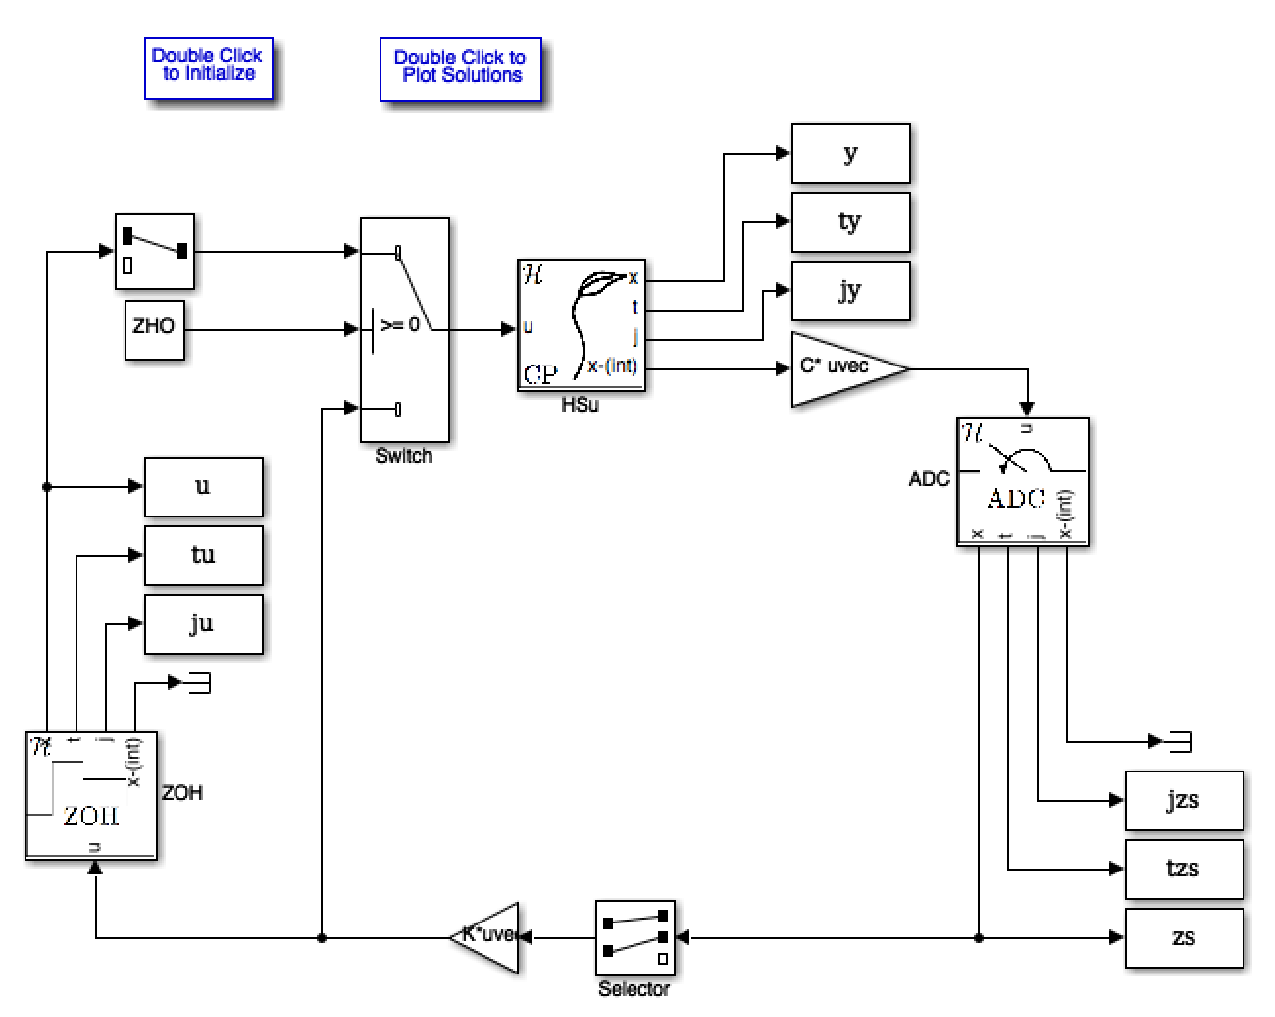
\includegraphics[width=0.8\textwidth]{figures/Simulink/SampleandHoldExample.eps}}
   \caption{Sample and hold feedback interconnection for Example~\ref{ex:S&Hcontrol}}
\label{fig:S&Hcontrol}
  \end{center}
\end{figure}

For each hybrid system in Figure~\ref{fig:S&Hcontrol} (HSu, ADC, and ZOH) we have the following Matlab embedded functions that describe the sets $C$ and $D$ and functions $f$ and $g$.
Figure~\ref{fig:ZOH_exampleResults} presents a numerical simulation of the interconnected system.

\begin{figure}%[ht]
  \begin{center}
    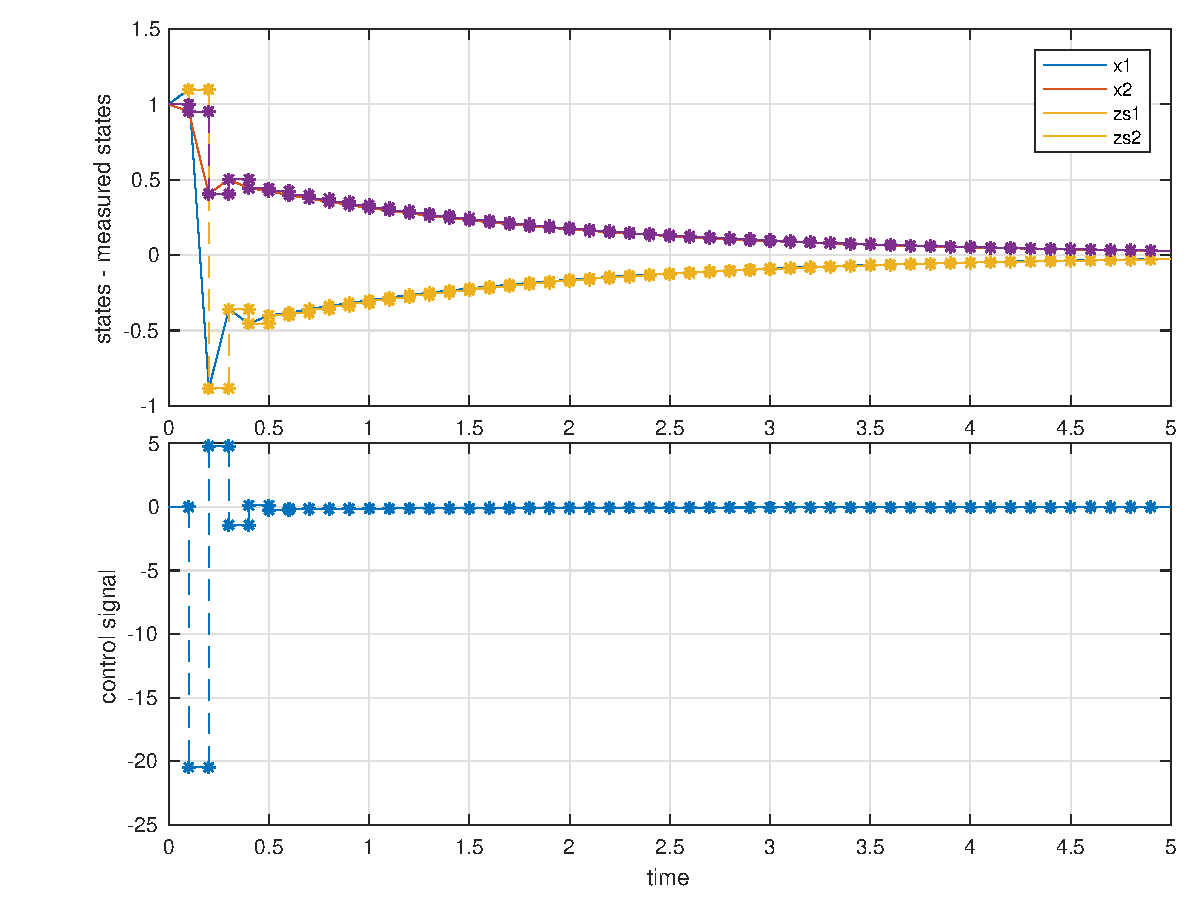
\includegraphics[width=0.8\textwidth]{figures/Simulink/ZOH_exampleResults.eps}
   \caption{Measuread states and inputs.}
\label{fig:ZOH_exampleResults}
  \end{center}
\end{figure}

% Set the location for MATLAB files included via the "\code" command.
\codeLocation{Matlab2tex_CPS_ContinuousPlant}

\begin{itemize}
\item Continuous process:

\code{f.m}
\code{C.m}
\code{g.m}
\code{D.m}

% Flow map
% %\scriptsize
% % This file was automatically created from the m-file 
% "m2tex.m" written by USL. 
% The fontencoding in this file is UTF-8. 
%  
% You will need to include the following two packages in 
% your LaTeX-Main-File. 
%  
% \usepackage{color} 
% \usepackage{fancyvrb} 
%  
% It is advised to use the following option for Inputenc 
% \usepackage[utf8]{inputenc} 
%  
  
% definition of matlab colors: 
\definecolor{mblue}{rgb}{0,0,1} 
\definecolor{mgreen}{rgb}{0.13333,0.5451,0.13333} 
\definecolor{mred}{rgb}{0.62745,0.12549,0.94118} 
\definecolor{mgrey}{rgb}{0.5,0.5,0.5} 
\definecolor{mdarkgrey}{rgb}{0.25,0.25,0.25} 
  
\DefineShortVerb[fontfamily=courier,fontseries=m]{\$} 
\DefineShortVerb[fontfamily=courier,fontseries=b]{\#} 
  
\noindent                    
 \hspace*{-1.6em}{\scriptsize 1}$  $\color{mblue}$function$\color{black}$ xdot = f(x, u, gamma)$\\
 \hspace*{-1.6em}{\scriptsize 2}$  $\\
 \hspace*{-1.6em}{\scriptsize 3}$  $\color{mgreen}#%%%%%%%%%%%%%%%%%%%%%%%%%%%%%%%%%%%%%%%%%%%%%%%%%%%%%%%%%%%%%%%%%%%%%%%%%%%#\color{black}$$\\
 \hspace*{-1.6em}{\scriptsize 4}$  $\color{mgreen}$% Matlab Function  Author: Ricardo Sanfelice $\color{black}$$\\
 \hspace*{-1.6em}{\scriptsize 5}$  $\color{mgreen}$% (Revised by Giampiero Campa)$\color{black}$$\\
 \hspace*{-1.6em}{\scriptsize 6}$  $\color{mgreen}$% (Revised by Pablo Nanez)$\color{black}$$\\
 \hspace*{-1.6em}{\scriptsize 7}$  $\color{mgreen}$%$\color{black}$$\\
 \hspace*{-1.6em}{\scriptsize 8}$  $\color{mgreen}$% Project: Simulation of a hybrid system (Bouncing Ball)$\color{black}$$\\
 \hspace*{-1.6em}{\scriptsize 9}$  $\color{mgreen}$%$\color{black}$$\\
 \hspace*{-2em}{\scriptsize 10}$  $\color{mgreen}$% Name: f.m$\color{black}$$\\
 \hspace*{-2em}{\scriptsize 11}$  $\color{mgreen}$%$\color{black}$$\\
 \hspace*{-2em}{\scriptsize 12}$  $\color{mgreen}$% Description: Flow map$\color{black}$$\\
 \hspace*{-2em}{\scriptsize 13}$  $\color{mgreen}$%$\color{black}$$\\
 \hspace*{-2em}{\scriptsize 14}$  $\color{mgreen}$% Version: 1.0$\color{black}$$\\
 \hspace*{-2em}{\scriptsize 15}$  $\color{mgreen}$% Required files: - $\color{black}$$\\
 \hspace*{-2em}{\scriptsize 16}$  $\color{mgreen}#%%%%%%%%%%%%%%%%%%%%%%%%%%%%%%%%%%%%%%%%%%%%%%%%%%%%%%%%%%%%%%%%%%%%%%%%%%%#\color{black}$$\\
 \hspace*{-2em}{\scriptsize 17}$  $\\
 \hspace*{-2em}{\scriptsize 18}$  $\\
 \hspace*{-2em}{\scriptsize 19}$  $\color{mgreen}$% flow map: xdot=f(x,u);$\color{black}$$\\
 \hspace*{-2em}{\scriptsize 20}$  xdot = [x(2); gamma];$\\ 
  
\UndefineShortVerb{\$} 
\UndefineShortVerb{\#}\label{scr:f}
% %\normalsize

% Flow set
% %\scriptsize
% % This file was automatically created from the m-file 
% "m2tex.m" written by USL. 
% The fontencoding in this file is UTF-8. 
%  
% You will need to include the following two packages in 
% your LaTeX-Main-File. 
%  
% \usepackage{color} 
% \usepackage{fancyvrb} 
%  
% It is advised to use the following option for Inputenc 
% \usepackage[utf8]{inputenc} 
%  
  
% definition of matlab colors: 
\definecolor{mblue}{rgb}{0,0,1} 
\definecolor{mgreen}{rgb}{0.13333,0.5451,0.13333} 
\definecolor{mred}{rgb}{0.62745,0.12549,0.94118} 
\definecolor{mgrey}{rgb}{0.5,0.5,0.5} 
\definecolor{mdarkgrey}{rgb}{0.25,0.25,0.25} 
  
\DefineShortVerb[fontfamily=courier,fontseries=m]{\$} 
\DefineShortVerb[fontfamily=courier,fontseries=b]{\#} 
  
\noindent                          
 \hspace*{-1.6em}{\scriptsize 1}$  $\color{mblue}$function$\color{black}$ v  = C(x, u)$\\
 \hspace*{-1.6em}{\scriptsize 2}$  $\color{mgreen}$%--------------------------------------------------------------------------$\color{black}$$\\
 \hspace*{-1.6em}{\scriptsize 3}$  $\color{mgreen}$% Matlab M-file Project: HyEQ Toolbox @  Hybrid Systems Laboratory (HSL),$\color{black}$$\\
 \hspace*{-1.6em}{\scriptsize 4}$  $\color{mgreen}$% https://hybrid.soe.ucsc.edu/software$\color{black}$$\\
 \hspace*{-1.6em}{\scriptsize 5}$  $\color{mgreen}$% http://hybridsimulator.wordpress.com/$\color{black}$$\\
 \hspace*{-1.6em}{\scriptsize 6}$  $\color{mgreen}$%--------------------------------------------------------------------------$\color{black}$$\\
 \hspace*{-1.6em}{\scriptsize 7}$  $\color{mgreen}$% Project: Simulation of a hybrid system$\color{black}$$\\
 \hspace*{-1.6em}{\scriptsize 8}$  $\color{mgreen}$% Description: Flow set$\color{black}$$\\
 \hspace*{-1.6em}{\scriptsize 9}$  $\color{mgreen}$%--------------------------------------------------------------------------$\color{black}$$\\
 \hspace*{-2em}{\scriptsize 10}$  $\color{mgreen}$%--------------------------------------------------------------------------$\color{black}$$\\
 \hspace*{-2em}{\scriptsize 11}$  $\color{mgreen}$%   See also HYEQSOLVER, PLOTARC, PLOTARC3, PLOTFLOWS, PLOTHARC,$\color{black}$$\\
 \hspace*{-2em}{\scriptsize 12}$  $\color{mgreen}$%   PLOTHARCCOLOR, PLOTHARCCOLOR3D, PLOTHYBRIDARC, PLOTJUMPS.$\color{black}$$\\
 \hspace*{-2em}{\scriptsize 13}$  $\color{mgreen}$%   Copyright @ Hybrid Systems Laboratory (HSL),$\color{black}$$\\
 \hspace*{-2em}{\scriptsize 14}$  $\color{mgreen}$%   Revision: 0.0.0.3 Date: 05/20/2015 3:42:00$\color{black}$$\\
 \hspace*{-2em}{\scriptsize 15}$  $\color{mgreen}$%$\color{black}$$\\
 \hspace*{-2em}{\scriptsize 16}$  $\color{mgreen}$% Check on flow conditions$\color{black}$$\\
 \hspace*{-2em}{\scriptsize 17}$  $\color{mgreen}$% E.g.,$\color{black}$$\\
 \hspace*{-2em}{\scriptsize 18}$  $\color{mgreen}$% if (x(1) >= u(1))  % flow condition$\color{black}$$\\
 \hspace*{-2em}{\scriptsize 19}$  $\color{mgreen}$%     v = 1;  % report flow$\color{black}$$\\
 \hspace*{-2em}{\scriptsize 20}$  $\color{mgreen}$% else$\color{black}$$\\
 \hspace*{-2em}{\scriptsize 21}$  $\color{mgreen}$%     v = 0;   % do not report flow$\color{black}$$\\
 \hspace*{-2em}{\scriptsize 22}$  $\color{mgreen}$% end$\color{black}$$\\
 \hspace*{-2em}{\scriptsize 23}$  $\\
 \hspace*{-2em}{\scriptsize 24}$  $\\
 \hspace*{-2em}{\scriptsize 25}$  v = 1; $\color{mgreen}$% report flow$\color{black}$$\\
 \hspace*{-2em}{\scriptsize 26}$  $\\ 
  
\UndefineShortVerb{\$} 
\UndefineShortVerb{\#}\label{scr:C}
% %\normalsize

% Jump map
% %\scriptsize
% % This file was automatically created from the m-file 
% "m2tex.m" written by USL. 
% The fontencoding in this file is UTF-8. 
%  
% You will need to include the following two packages in 
% your LaTeX-Main-File. 
%  
% \usepackage{color} 
% \usepackage{fancyvrb} 
%  
% It is advised to use the following option for Inputenc 
% \usepackage[utf8]{inputenc} 
%  
  
% definition of matlab colors: 
\definecolor{mblue}{rgb}{0,0,1} 
\definecolor{mgreen}{rgb}{0.13333,0.5451,0.13333} 
\definecolor{mred}{rgb}{0.62745,0.12549,0.94118} 
\definecolor{mgrey}{rgb}{0.5,0.5,0.5} 
\definecolor{mdarkgrey}{rgb}{0.25,0.25,0.25} 
  
\DefineShortVerb[fontfamily=courier,fontseries=m]{\$} 
\DefineShortVerb[fontfamily=courier,fontseries=b]{\#} 
  
\noindent   
 \hspace*{-1.6em}{\scriptsize 1}$  $\color{mblue}$function$\color{black}$ xplus = g(x, u, lambda)$\\
 \hspace*{-1.6em}{\scriptsize 2}$  $\color{mgreen}$% jump map$\color{black}$$\\
 \hspace*{-1.6em}{\scriptsize 3}$  xplus = [u(1); -lambda*x(2)];$\\ 
  
\UndefineShortVerb{\$} 
\UndefineShortVerb{\#}\label{scr:g}
% %\normalsize

% Jump set
% %\scriptsize
% % This file was automatically created from the m-file 
% "m2tex.m" written by USL. 
% The fontencoding in this file is UTF-8. 
%  
% You will need to include the following two packages in 
% your LaTeX-Main-File. 
%  
% \usepackage{color} 
% \usepackage{fancyvrb} 
%  
% It is advised to use the following option for Inputenc 
% \usepackage[utf8]{inputenc} 
%  
  
% definition of matlab colors: 
\definecolor{mblue}{rgb}{0,0,1} 
\definecolor{mgreen}{rgb}{0.13333,0.5451,0.13333} 
\definecolor{mred}{rgb}{0.62745,0.12549,0.94118} 
\definecolor{mgrey}{rgb}{0.5,0.5,0.5} 
\definecolor{mdarkgrey}{rgb}{0.25,0.25,0.25} 
  
\DefineShortVerb[fontfamily=courier,fontseries=m]{\$} 
\DefineShortVerb[fontfamily=courier,fontseries=b]{\#} 
  
\noindent                         
 \hspace*{-1.6em}{\scriptsize 1}$  $\color{mblue}$function$\color{black}$ v  = D(x, u) $\\
 \hspace*{-1.6em}{\scriptsize 2}$  $\\
 \hspace*{-1.6em}{\scriptsize 3}$  $\color{mgreen}#%%%%%%%%%%%%%%%%%%%%%%%%%%%%%%%%%%%%%%%%%%%%%%%%%%%%%%%%%%%%%%%%%%%%%%%%%%%#\color{black}$$\\
 \hspace*{-1.6em}{\scriptsize 4}$  $\color{mgreen}$% Matlab Function  Author: Ricardo Sanfelice $\color{black}$$\\
 \hspace*{-1.6em}{\scriptsize 5}$  $\color{mgreen}$% (Revised by Giampiero Campa)$\color{black}$$\\
 \hspace*{-1.6em}{\scriptsize 6}$  $\color{mgreen}$% (Revised by Pablo Nanez)$\color{black}$$\\
 \hspace*{-1.6em}{\scriptsize 7}$  $\color{mgreen}$%$\color{black}$$\\
 \hspace*{-1.6em}{\scriptsize 8}$  $\color{mgreen}$% Project: Simulation of a hybrid system (Bouncing ball)$\color{black}$$\\
 \hspace*{-1.6em}{\scriptsize 9}$  $\color{mgreen}$%$\color{black}$$\\
 \hspace*{-2em}{\scriptsize 10}$  $\color{mgreen}$% Name: D.m$\color{black}$$\\
 \hspace*{-2em}{\scriptsize 11}$  $\color{mgreen}$%$\color{black}$$\\
 \hspace*{-2em}{\scriptsize 12}$  $\color{mgreen}$% Description: Jump set$\color{black}$$\\
 \hspace*{-2em}{\scriptsize 13}$  $\color{mgreen}$%$\color{black}$$\\
 \hspace*{-2em}{\scriptsize 14}$  $\color{mgreen}$% Version: 1.0$\color{black}$$\\
 \hspace*{-2em}{\scriptsize 15}$  $\color{mgreen}$% Required files: - $\color{black}$$\\
 \hspace*{-2em}{\scriptsize 16}$  $\color{mgreen}#%%%%%%%%%%%%%%%%%%%%%%%%%%%%%%%%%%%%%%%%%%%%%%%%%%%%%%%%%%%%%%%%%%%%%%%%%%%#\color{black}$$\\
 \hspace*{-2em}{\scriptsize 17}$  $\\
 \hspace*{-2em}{\scriptsize 18}$  xtemp = zeros(2,1);$\\
 \hspace*{-2em}{\scriptsize 19}$  xtemp = x;$\\
 \hspace*{-2em}{\scriptsize 20}$  $\\
 \hspace*{-2em}{\scriptsize 21}$  $\color{mblue}$if$\color{black}$ (xtemp(1) <= u(1)) && (xtemp(2) <= 0)  $\color{mgreen}$% jump condition$\color{black}$$\\
 \hspace*{-2em}{\scriptsize 22}$      v = 1;  $\color{mgreen}$% report jump$\color{black}$$\\
 \hspace*{-2em}{\scriptsize 23}$  $\color{mblue}$else$\color{black}$$\\
 \hspace*{-2em}{\scriptsize 24}$      v = 0;   $\color{mgreen}$% do not report jump$\color{black}$$\\
 \hspace*{-2em}{\scriptsize 25}$  $\color{mblue}$end$\color{black}$$\\ 
  
\UndefineShortVerb{\$} 
\UndefineShortVerb{\#}\label{scr:D}
% %\normalsize
\item ADC and ZOH:

\code{f\_ADC.m}
\code{C\_ADC.m}
\code{g\_ADC.m}
\code{D\_ADC.m}

% Flow map
% %\scriptsize
% % This file was automatically created from the m-file 
% "m2tex.m" written by USL. 
% The fontencoding in this file is UTF-8. 
%  
% You will need to include the following two packages in 
% your LaTeX-Main-File. 
%  
% \usepackage{color} 
% \usepackage{fancyvrb} 
%  
% It is advised to use the following option for Inputenc 
% \usepackage[utf8]{inputenc} 
%  
  
% definition of matlab colors: 
\definecolor{mblue}{rgb}{0,0,1} 
\definecolor{mgreen}{rgb}{0.13333,0.5451,0.13333} 
\definecolor{mred}{rgb}{0.62745,0.12549,0.94118} 
\definecolor{mgrey}{rgb}{0.5,0.5,0.5} 
\definecolor{mdarkgrey}{rgb}{0.25,0.25,0.25} 
  
\DefineShortVerb[fontfamily=courier,fontseries=m]{\$} 
\DefineShortVerb[fontfamily=courier,fontseries=b]{\#} 
  
\noindent                     
 \hspace*{-1.6em}{\scriptsize 1}$  $\color{mblue}$function$\color{black}$ xdot = f(x,vs)$\\
 \hspace*{-1.6em}{\scriptsize 2}$  $\color{mgreen}$%--------------------------------------------------------------------------$\color{black}$$\\
 \hspace*{-1.6em}{\scriptsize 3}$  $\color{mgreen}$% Matlab M-file Project: HyEQ Toolbox @  Hybrid Systems Laboratory (HSL), $\color{black}$$\\
 \hspace*{-1.6em}{\scriptsize 4}$  $\color{mgreen}$% https://hybrid.soe.ucsc.edu/software$\color{black}$$\\
 \hspace*{-1.6em}{\scriptsize 5}$  $\color{mgreen}$% http://hybridsimulator.wordpress.com/$\color{black}$$\\
 \hspace*{-1.6em}{\scriptsize 6}$  $\color{mgreen}$%--------------------------------------------------------------------------$\color{black}$$\\
 \hspace*{-1.6em}{\scriptsize 7}$  $\color{mgreen}$% Project: Simulation of a hybrid system Analog-to-Digital converter (ADC) $\color{black}$$\\
 \hspace*{-1.6em}{\scriptsize 8}$  $\color{mgreen}$% Description: Flow map$\color{black}$$\\
 \hspace*{-1.6em}{\scriptsize 9}$  $\color{mgreen}$%--------------------------------------------------------------------------$\color{black}$$\\
 \hspace*{-2em}{\scriptsize 10}$  $\color{mgreen}$%--------------------------------------------------------------------------$\color{black}$$\\
 \hspace*{-2em}{\scriptsize 11}$  $\color{mgreen}$%   See also HYEQSOLVER, PLOTARC, PLOTARC3, PLOTFLOWS, PLOTHARC,$\color{black}$$\\
 \hspace*{-2em}{\scriptsize 12}$  $\color{mgreen}$%   PLOTHARCCOLOR, PLOTHARCCOLOR3D, PLOTHYBRIDARC, PLOTJUMPS.$\color{black}$$\\
 \hspace*{-2em}{\scriptsize 13}$  $\color{mgreen}$%   Copyright @ Hybrid Systems Laboratory (HSL),$\color{black}$$\\
 \hspace*{-2em}{\scriptsize 14}$  $\color{mgreen}$%   Revision: 0.0.0.3 Date: 05/20/2015 3:42:00$\color{black}$$\\
 \hspace*{-2em}{\scriptsize 15}$  $\\
 \hspace*{-2em}{\scriptsize 16}$  n = length(vs); $\color{mgreen}$% measured input size$\color{black}$$\\
 \hspace*{-2em}{\scriptsize 17}$  $\\
 \hspace*{-2em}{\scriptsize 18}$  msdot = zeros(n,1); $\color{mgreen}$% measured continuous dynamics$\color{black}$$\\
 \hspace*{-2em}{\scriptsize 19}$  tau_sdot = 1; $\color{mgreen}$% Timer tau_s$\color{black}$$\\
 \hspace*{-2em}{\scriptsize 20}$  xdot = [msdot;tau_sdot];$\\
 \hspace*{-2em}{\scriptsize 21}$  $\\ 
  
\UndefineShortVerb{\$} 
\UndefineShortVerb{\#}\label{scr:f}
% %\normalsize

% Flow set
% %\scriptsize
% % This file was automatically created from the m-file 
% "m2tex.m" written by USL. 
% The fontencoding in this file is UTF-8. 
%  
% You will need to include the following two packages in 
% your LaTeX-Main-File. 
%  
% \usepackage{color} 
% \usepackage{fancyvrb} 
%  
% It is advised to use the following option for Inputenc 
% \usepackage[utf8]{inputenc} 
%  
  
% definition of matlab colors: 
\definecolor{mblue}{rgb}{0,0,1} 
\definecolor{mgreen}{rgb}{0.13333,0.5451,0.13333} 
\definecolor{mred}{rgb}{0.62745,0.12549,0.94118} 
\definecolor{mgrey}{rgb}{0.5,0.5,0.5} 
\definecolor{mdarkgrey}{rgb}{0.25,0.25,0.25} 
  
\DefineShortVerb[fontfamily=courier,fontseries=m]{\$} 
\DefineShortVerb[fontfamily=courier,fontseries=b]{\#} 
  
\noindent                                  
 \hspace*{-1.6em}{\scriptsize 1}$  $\color{mblue}$function$\color{black}$ v  = C(x, vs, Ts) $\\
 \hspace*{-1.6em}{\scriptsize 2}$  $\color{mgreen}$%--------------------------------------------------------------------------$\color{black}$$\\
 \hspace*{-1.6em}{\scriptsize 3}$  $\color{mgreen}$% Matlab M-file Project: HyEQ Toolbox @  Hybrid Systems Laboratory (HSL), $\color{black}$$\\
 \hspace*{-1.6em}{\scriptsize 4}$  $\color{mgreen}$% https://hybrid.soe.ucsc.edu/software$\color{black}$$\\
 \hspace*{-1.6em}{\scriptsize 5}$  $\color{mgreen}$% http://hybridsimulator.wordpress.com/$\color{black}$$\\
 \hspace*{-1.6em}{\scriptsize 6}$  $\color{mgreen}$%--------------------------------------------------------------------------$\color{black}$$\\
 \hspace*{-1.6em}{\scriptsize 7}$  $\color{mgreen}$% Project: Simulation of a hybrid system Analog-to-Digital converter (ADC) $\color{black}$$\\
 \hspace*{-1.6em}{\scriptsize 8}$  $\color{mgreen}$% Description: Flow set$\color{black}$$\\
 \hspace*{-1.6em}{\scriptsize 9}$  $\color{mgreen}$%--------------------------------------------------------------------------$\color{black}$$\\
 \hspace*{-2em}{\scriptsize 10}$  $\color{mgreen}$%--------------------------------------------------------------------------$\color{black}$$\\
 \hspace*{-2em}{\scriptsize 11}$  $\color{mgreen}$%   See also HYEQSOLVER, PLOTARC, PLOTARC3, PLOTFLOWS, PLOTHARC,$\color{black}$$\\
 \hspace*{-2em}{\scriptsize 12}$  $\color{mgreen}$%   PLOTHARCCOLOR, PLOTHARCCOLOR3D, PLOTHYBRIDARC, PLOTJUMPS.$\color{black}$$\\
 \hspace*{-2em}{\scriptsize 13}$  $\color{mgreen}$%   Copyright @ Hybrid Systems Laboratory (HSL),$\color{black}$$\\
 \hspace*{-2em}{\scriptsize 14}$  $\color{mgreen}$%   Revision: 0.0.0.3 Date: 05/20/2015 3:42:00$\color{black}$$\\
 \hspace*{-2em}{\scriptsize 15}$  $\color{mgreen}$%$\color{black}$$\\
 \hspace*{-2em}{\scriptsize 16}$  $\color{mgreen}$% Check on flow conditions$\color{black}$$\\
 \hspace*{-2em}{\scriptsize 17}$  $\color{mgreen}$% E.g.,$\color{black}$$\\
 \hspace*{-2em}{\scriptsize 18}$  $\color{mgreen}$% if (x(1) >= u(1))  % flow condition$\color{black}$$\\
 \hspace*{-2em}{\scriptsize 19}$  $\color{mgreen}$%     v = 1;  % report flow$\color{black}$$\\
 \hspace*{-2em}{\scriptsize 20}$  $\color{mgreen}$% else$\color{black}$$\\
 \hspace*{-2em}{\scriptsize 21}$  $\color{mgreen}$%     v = 0;   % do not report flow$\color{black}$$\\
 \hspace*{-2em}{\scriptsize 22}$  $\color{mgreen}$% end$\color{black}$$\\
 \hspace*{-2em}{\scriptsize 23}$  $\\
 \hspace*{-2em}{\scriptsize 24}$  n = length(vs); $\color{mgreen}$% measured input size$\color{black}$$\\
 \hspace*{-2em}{\scriptsize 25}$  $\\
 \hspace*{-2em}{\scriptsize 26}$  tau_s = x(end); $\color{mgreen}$% timer state$\color{black}$$\\
 \hspace*{-2em}{\scriptsize 27}$  $\\
 \hspace*{-2em}{\scriptsize 28}$  $\color{mblue}$if$\color{black}$ tau_s>=0 && tau_s<= Ts$\\
 \hspace*{-2em}{\scriptsize 29}$      v = 1; $\color{mgreen}$% report flow$\color{black}$$\\
 \hspace*{-2em}{\scriptsize 30}$  $\color{mblue}$elseif$\color{black}$ tau_s> Ts$\\
 \hspace*{-2em}{\scriptsize 31}$      v = 0; $\color{mgreen}$% do not report flow$\color{black}$$\\
 \hspace*{-2em}{\scriptsize 32}$  $\color{mblue}$else$\color{black}$$\\
 \hspace*{-2em}{\scriptsize 33}$      v = 0;$\\
 \hspace*{-2em}{\scriptsize 34}$  $\color{mblue}$end$\color{black}$$\\ 
  
\UndefineShortVerb{\$} 
\UndefineShortVerb{\#}\label{scr:C}
% %\normalsize

% Jump map
% %\scriptsize
% % This file was automatically created from the m-file 
% "m2tex.m" written by USL. 
% The fontencoding in this file is UTF-8. 
%  
% You will need to include the following two packages in 
% your LaTeX-Main-File. 
%  
% \usepackage{color} 
% \usepackage{fancyvrb} 
%  
% It is advised to use the following option for Inputenc 
% \usepackage[utf8]{inputenc} 
%  
  
% definition of matlab colors: 
\definecolor{mblue}{rgb}{0,0,1} 
\definecolor{mgreen}{rgb}{0.13333,0.5451,0.13333} 
\definecolor{mred}{rgb}{0.62745,0.12549,0.94118} 
\definecolor{mgrey}{rgb}{0.5,0.5,0.5} 
\definecolor{mdarkgrey}{rgb}{0.25,0.25,0.25} 
  
\DefineShortVerb[fontfamily=courier,fontseries=m]{\$} 
\DefineShortVerb[fontfamily=courier,fontseries=b]{\#} 
  
\begin{Verbatim}[commandchars=\$\{\},numbers=left,numbersep=2pt] 

    $textcolor{mblue}{function} xplus = g(x, vs) 
    $textcolor{mgreen}{%--------------------------------------------------------------------------} 
    $textcolor{mgreen}{% Matlab M-file Project: HyEQ Toolbox @  Hybrid Systems Laboratory (HSL), } 
    $textcolor{mgreen}{% https://hybrid.soe.ucsc.edu/software} 
    $textcolor{mgreen}{% http://hybridsimulator.wordpress.com/} 
    $textcolor{mgreen}{%--------------------------------------------------------------------------} 
    $textcolor{mgreen}{% Project: Simulation of a hybrid system Analog-to-Digital converter (ADC) } 
    $textcolor{mgreen}{% Description: Jump map} 
    $textcolor{mgreen}{%--------------------------------------------------------------------------} 
    $textcolor{mgreen}{%--------------------------------------------------------------------------} 
    $textcolor{mgreen}{%   See also HYEQSOLVER, PLOTARC, PLOTARC3, PLOTFLOWS, PLOTHARC,} 
    $textcolor{mgreen}{%   PLOTHARCCOLOR, PLOTHARCCOLOR3D, PLOTHYBRIDARC, PLOTJUMPS.} 
    $textcolor{mgreen}{%   Copyright @ Hybrid Systems Laboratory (HSL),} 
    $textcolor{mgreen}{%   Revision: 0.0.0.3 Date: 05/20/2015 3:42:00} 
     
     
    n = length(vs) $textcolor{mgreen}{% measured input size} 
     
    msplus = vs; $textcolor{mgreen}{% output = measured input} 
    tau_splus = 0; $textcolor{mgreen}{% Timer tau_s} 
    xplus = [msplus;tau_splus]; 
     
     
      
\end{Verbatim}  
  
\UndefineShortVerb{\$} 
\UndefineShortVerb{\#} 
 \label{scr:g}
% %\normalsize

% Jump set
% %\scriptsize
% % This file was automatically created from the m-file 
% "m2tex.m" written by USL. 
% The fontencoding in this file is UTF-8. 
%  
% You will need to include the following two packages in 
% your LaTeX-Main-File. 
%  
% \usepackage{color} 
% \usepackage{fancyvrb} 
%  
% It is advised to use the following option for Inputenc 
% \usepackage[utf8]{inputenc} 
%  
  
% definition of matlab colors: 
\definecolor{mblue}{rgb}{0,0,1} 
\definecolor{mgreen}{rgb}{0.13333,0.5451,0.13333} 
\definecolor{mred}{rgb}{0.62745,0.12549,0.94118} 
\definecolor{mgrey}{rgb}{0.5,0.5,0.5} 
\definecolor{mdarkgrey}{rgb}{0.25,0.25,0.25} 
  
\DefineShortVerb[fontfamily=courier,fontseries=m]{\$} 
\DefineShortVerb[fontfamily=courier,fontseries=b]{\#} 
  
\noindent                                  
 \hspace*{-1.6em}{\scriptsize 1}$  $\color{mblue}$function$\color{black}$ v  = D(x, vs, Ts) $\\
 \hspace*{-1.6em}{\scriptsize 2}$  $\color{mgreen}$%--------------------------------------------------------------------------$\color{black}$$\\
 \hspace*{-1.6em}{\scriptsize 3}$  $\color{mgreen}$% Matlab M-file Project: HyEQ Toolbox @  Hybrid Systems Laboratory (HSL), $\color{black}$$\\
 \hspace*{-1.6em}{\scriptsize 4}$  $\color{mgreen}$% https://hybrid.soe.ucsc.edu/software$\color{black}$$\\
 \hspace*{-1.6em}{\scriptsize 5}$  $\color{mgreen}$% http://hybridsimulator.wordpress.com/$\color{black}$$\\
 \hspace*{-1.6em}{\scriptsize 6}$  $\color{mgreen}$%--------------------------------------------------------------------------$\color{black}$$\\
 \hspace*{-1.6em}{\scriptsize 7}$  $\color{mgreen}$% Project: Simulation of a hybrid system Analog-to-Digital converter (ADC) $\color{black}$$\\
 \hspace*{-1.6em}{\scriptsize 8}$  $\color{mgreen}$% Description: Jump set$\color{black}$$\\
 \hspace*{-1.6em}{\scriptsize 9}$  $\color{mgreen}$%--------------------------------------------------------------------------$\color{black}$$\\
 \hspace*{-2em}{\scriptsize 10}$  $\color{mgreen}$%--------------------------------------------------------------------------$\color{black}$$\\
 \hspace*{-2em}{\scriptsize 11}$  $\color{mgreen}$%   See also HYEQSOLVER, PLOTARC, PLOTARC3, PLOTFLOWS, PLOTHARC,$\color{black}$$\\
 \hspace*{-2em}{\scriptsize 12}$  $\color{mgreen}$%   PLOTHARCCOLOR, PLOTHARCCOLOR3D, PLOTHYBRIDARC, PLOTJUMPS.$\color{black}$$\\
 \hspace*{-2em}{\scriptsize 13}$  $\color{mgreen}$%   Copyright @ Hybrid Systems Laboratory (HSL),$\color{black}$$\\
 \hspace*{-2em}{\scriptsize 14}$  $\color{mgreen}$%   Revision: 0.0.0.3 Date: 05/20/2015 3:42:00$\color{black}$$\\
 \hspace*{-2em}{\scriptsize 15}$  $\color{mgreen}$%$\color{black}$$\\
 \hspace*{-2em}{\scriptsize 16}$  $\color{mgreen}$% Check on jump conditions$\color{black}$$\\
 \hspace*{-2em}{\scriptsize 17}$  $\color{mgreen}$% % E.g.,$\color{black}$$\\
 \hspace*{-2em}{\scriptsize 18}$  $\color{mgreen}$% if (x(1) <= u(1)) && (x(2) <= 0)  % jump condition$\color{black}$$\\
 \hspace*{-2em}{\scriptsize 19}$  $\color{mgreen}$%     v = 1;  % report jump$\color{black}$$\\
 \hspace*{-2em}{\scriptsize 20}$  $\color{mgreen}$% else$\color{black}$$\\
 \hspace*{-2em}{\scriptsize 21}$  $\color{mgreen}$%     v = 0;   % do not report jump$\color{black}$$\\
 \hspace*{-2em}{\scriptsize 22}$  $\color{mgreen}$% end$\color{black}$$\\
 \hspace*{-2em}{\scriptsize 23}$  $\\
 \hspace*{-2em}{\scriptsize 24}$  n = length(vs); $\color{mgreen}$% measured input size$\color{black}$$\\
 \hspace*{-2em}{\scriptsize 25}$  $\\
 \hspace*{-2em}{\scriptsize 26}$  tau_s = x(end); $\color{mgreen}$% timer state$\color{black}$$\\
 \hspace*{-2em}{\scriptsize 27}$  $\\
 \hspace*{-2em}{\scriptsize 28}$  $\color{mblue}$if$\color{black}$ tau_s>=0 && tau_s<= Ts$\\
 \hspace*{-2em}{\scriptsize 29}$      v = 0; $\color{mgreen}$% do not report jump$\color{black}$$\\
 \hspace*{-2em}{\scriptsize 30}$  $\color{mblue}$elseif$\color{black}$ tau_s> Ts$\\
 \hspace*{-2em}{\scriptsize 31}$      v = 1; $\color{mgreen}$% report jump$\color{black}$$\\
 \hspace*{-2em}{\scriptsize 32}$  $\color{mblue}$else$\color{black}$$\\
 \hspace*{-2em}{\scriptsize 33}$      v = 0;$\\
 \hspace*{-2em}{\scriptsize 34}$  $\color{mblue}$end$\color{black}$$\\ 
  
\UndefineShortVerb{\$} 
\UndefineShortVerb{\#}\label{scr:D}
% %\normalsize
\end{itemize}

There are numerous practical examples of systems that can be modeled 
within the general model for sample-and-hold feedback control defined above.
For example, one ``classical'' example is the control of the temperature of a room 
by turning on and off a heater so as to keep the temperature within a desired range\NotSAE{; see the model in \eqref{eqn:TemperatureModel}}.
Another widely known example is the control of the level of a water tank.

\end{example}



\section{Further Reading}
\label{sec:closingremarks}
\noindent Installation files for the HyEQ Toolbox described in this paper can be found 
at \matlab{} Central and at the author's website
\begin{center}
\url{https://hybrid.soe.ucsc.edu/software}.
\end{center}
Also, resources and examples are shared by the HyEQ Toolbox users in the blog
\begin{center}
\url{http://hybridsimulator.wordpress.com}.
\end{center}

\section{Acknowledgments}
\label{sec:acknowledgments}

We would like to thank Giampiero Campa for his thoughtful feedback 
and advice as well as Torstein Ingebrigtsen Bo for his comments 
and initial version of the \matlab{}-based simulator code, 
and the following list of people who have helped to test this toolbox:

\begin{itemize}
\item Cenk Oguz Saglam - University of California, Santa Barbara
\item Bharani Malladi - The University of Arizona
\end{itemize}

\bibliographystyle{unsrt} 
\bibliography{biblio}\label{sec:refs}

\include{foot}

\end{document}
